\documentclass[11pt]{book}
\oddsidemargin 0in
\evensidemargin 0in
\marginparwidth 0in
\textheight 8in
\textwidth 6.5in
\topmargin 0in
\headheight 14pt
\usepackage{amssymb,amsmath,amsthm,fancyhdr,supertabular,longtable,hhline,mathtools}
\usepackage{colortbl}
\usepackage{import, multicol,boxedminipage}
\usepackage{chapterfolder}
\usepackage[metapost,truebbox]{mfpic}
\usepackage[pdflatex]{graphicx}
\usepackage{makeidx}
\usepackage[colorlinks, hyperindex, plainpages=false, linkcolor=blue, urlcolor=blue, pdfpagelabels]{hyperref}
\usepackage[all]{hypcap}
\usepackage{cancel}
\usepackage{sectsty}
\usepackage{textcomp}
\allsectionsfont{\mdseries \scshape}
\definecolor{ResultColor}{gray}{0.9}
\theoremstyle{definition}  % this prevents the text in definitions, theorems, and corollaries from being italicized
\newtheorem{defn}{\sc Definition}[chapter]
\newtheorem{thm}{\sc Theorem}[chapter]
\newtheorem{cor}[thm]{\sc Corollary}
\newtheorem{eqn}{\sc Equation}[chapter]
\newtheorem{ex}{\sc Example}[section]
\newtheorem{fig}{\sc Figure}[chapter]
\setlength{\parindent}{0in}
\newcommand{\bbm}{\begin{boxedminipage}{6.41in}}
\newcommand{\ebm}{\end{boxedminipage}}
\usepackage{array}
\setlength{\extrarowheight}{2pt}
\allowdisplaybreaks[2]
\allsectionsfont{\mdseries \scshape}
%Below is for Helvetica (scaled): 
\usepackage[scaled=.92]{helvet}   
\renewcommand{\familydefault}{\sfdefault}  %makes the text of the book sans serif
\usepackage[helvet]{sfmath}  %makes the math in the book sans serif
\allsectionsfont{\sffamily}  %makes the chapter and section titles sans serif

\makeatletter
\newcases{mycases}{\quad}{%
  \hfil$\m@th\displaystyle{##}$}{$\m@th\displaystyle{##}$\hfil}{\lbrace}{.}
\makeatother

\begin{document}
\newcounter{HW}
\newcounter{HWindent}


\chapter{\sc Introduction to Functions}

\section{Functions and their Representations}

\mfpicnumber{1}

\opengraphsfile{FunctionsandtheirRepresentations}

\setcounter{footnote}{0}

\label{FunctionsandtheirRepresentations}


\subsection{Functions as Mappings}

Mathematics can be thought of as the study of patterns.   In most disciplines, Mathematics is used as a language to express, or codify, relationships between quantities  - both algebraically and geometrically - with the ultimate goal of solving real-world problems.   The fact that the same algebraic equation which models the growth of bacteria in a petri dish is also used to compute the account balance of a savings account or the potency of radioactive material used in medical treatments speaks to the universal nature of Mathematics.   Indeed, Mathematics is more than just about solving a specific problem in a specific situation, it's about abstracting problems and creating universal tools which can be used by a variety of scientists and engineers to solve a variety of problems.  

\medskip

This power of abstraction has a tendency to create a language that is initially intimidating to students.  Mathematical definitions are precise and adherence to that precision is often a source of confusion and frustration.  It doesn't help matters that more often than not very common words are used in Mathematics with slightly different definitions than is commonly expected.  The first `universal tool' we wish to highlight - the concept of a `function' - is a perfect example of this phenomenon in that we redefine a word that already has multiple meanings in English.  

\medskip

\colorbox{ResultColor}{\bbm

\begin{defn}

\label{functiondefn}

Given two sets\footnote{Please refer to Section \ref{AppSetTheory} for a review of this terminology.} $A$ and $B$, a  \index{function ! definition} \textbf{function} from $A$ to $B$ is a process by which each element of $A$ is matched with (or `mapped to')  one and only one element of $B$.   

\end{defn}

\ebm}

\medskip

The grammar here `\textit{from} $A$ \textit{to} $B\,$'  is important.  Thinking of a function as a process, we can view the elements of the set $A$ as our starting materials, or \textit{inputs} to the process.  The function  processes these inputs according to some specified rule and the result is a set of  \textit{outputs}  - elements of the set $B$. In terms of inputs and outputs, Definition \ref{functiondefn}  says that a function is a process in which each \textit{input} is matched to one and only one \textit{output}.

\medskip

For example, let's take a look at some of the pets in the Stitz household.  Taylor's pets include White Paw and Cooper (both cats), Bingo (a lizard) and Kennie (a turtle).  Let $N$ be the set of pet names: $N = \{ \text{White Paw, Cooper, Bingo, Kennie} \}$, and let $T$ be the set of pet types:  $T = \{ \text{cat, lizard, turtle} \}$.   Let $f$ be the process that takes each pet's name as the input and returns that pet's type as the output. Let $g$ be the reverse of $f$:  that is, $g$ takes each pet type as the input and returns the names of the pets of that type as the output.   Note that both $f$ and $g$ are codifying the \textit{same} given information about Taylor's pets,  but one of them is a function and the other is not.  

\medskip

To help identify which process $f$ or $g$ is a function and  why the other is not, we create  \index{diagram ! mapping} \textbf{mapping diagrams} for $f$ and $g$ below.  In each case, we organize the inputs in a column on the left and the outputs on a column on the right.  We draw an arrow connecting each input to its corresponding output(s).  Note that the arrows communicate the grammatical bias: the arrow originates at the input and points to the output.

\medskip

\begin{center}

\begin{tabular}{cc}
\begin{mfpic}[19]{-5}{5}{2}{6}
\tlabel[cc](-4.25,6){$N$ (inputs)}
\tlabel[cc](-4.25,5){White Paw}
\tlabel[cc](-4.25,4){Cooper}
\tlabel[cc](-4.25,3){Bingo}
\tlabel[cc](-4.25,2){Kennie}
\tlabel[cc](0,6){$f$}
\tlabel[cc](3.5,5){cat}
\tlabel[cc](3.5,4){lizard}
\tlabel[cc](3.5,3){turtle}
\tlabel[cc](3.5,6){$T$ (outputs)}


\arrow[l 5pt] \polyline{(-2.5, 5), (2.5, 5)}
\arrow[l 5pt] \polyline{(-2.5, 4), (2.5, 5)}
\arrow[l 5pt] \polyline{(-2.5, 3), (2.5, 4)}
\arrow[l 5pt] \polyline{(-2.5, 2), (2.5, 3)}

\end{mfpic}

&
\begin{mfpic}[19]{-5}{5}{2}{6}
\tlabel[cc](-3.5,6){$T$ (inputs)}
\tlabel[cc](-3.5,5){cat}
\tlabel[cc](-3.5,4){lizard}
\tlabel[cc](-3.5,3){turtle}
\tlabel[cc](0,6){$g$}
\tlabel[cc](3.75,6){$N$ (outputs)}
\tlabel[cc](3.75,5){White Paw}
\tlabel[cc](3.75,4){Cooper}
\tlabel[cc](3.75,3){Bingo}
\tlabel[cc](3.75,2){Kennie}
\arrow[l 5pt] \polyline{(-2.5, 5), (2.5, 5)}
\arrow[l 5pt] \polyline{(-2.5, 5), (2.5, 4)}
\arrow[l 5pt] \polyline{(-2.5, 4), (2.5, 3)}
\arrow[l 5pt] \polyline{(-2.5, 3), (2.5, 2)}
\end{mfpic}   \\

\end{tabular}

\end{center}

The process $f$ is a function since $f$ matches each of its inputs (each pet name) to just one output (the pet's type).   The fact that different inputs (White Paw and Cooper) are matched to the same output (cat) is fine.   On the other hand, $g$ matches the input `cat' to the two different outputs  `White Paw' and `Cooper', so $g$ is not a function.    Functions are favored in mathematical circles because they are processes which produce only one answer (output) for any given query (input).  In this scenario, for instance, there is only one answer to the question: `What type of pet is White Paw?' but there is more than one answer to the question `Which of Taylor's pets are cats?'  

\medskip

As you might expect, with functions being such an important concept in Mathematics, we need to build a vocabulary to assist us when discussing them.  To that end, we have the following definitions.\footnote{Please refer to Section \ref{AppSetTheory} for a review of the terminology used in these definitions.}

\medskip

\colorbox{ResultColor}{\bbm

\begin{defn}

\label{domainrangedefns}

Suppose $f$ is a function from $A$ to $B$.

\begin{itemize}

\item If $a \in A$, we write $f(a)$ (read `$f$ of $a\, $') to denote the unique element of $B$ to which $f$ matches $a$.  

That is, if we view `$a\,$' as the input to $f$, then `$f(a)$' is the output from $f$.

\item  The set $A$ is called the \index{domain ! definition} \textbf{domain}.  

Said differently, the domain of a function is the set of inputs to the function.

\item  The set $\{ f(a) \, | \, a \in A \}$ is called the  \index{range ! definition}  \textbf{range} of $f$. 

Said differently, the range of a function is the set of outputs from the function.

\end{itemize}


\end{defn}

\ebm}

Some remarks about Definition \ref{domainrangedefns} are in order.  First, and most importantly, the notation `$f(a)$' in Definition \ref{domainrangedefns}  introduces yet another mathematical use for parentheses.  Parentheses are used in some cases as grouping symbols, to represent ordered pairs, and to delineate intervals of real numbers.  More often than not, the use of parentheses in expressions like `$f(a)$' is confused with multiplication.   As always, paying attention to the context is key.  If $f$ is a function and `$a\,$' is in the domain of $f$, then `$f(a)$'  is the output from $f$ when you input $a$.  The diagram below provides a nice generic picture to keep in mind when thinking of a function as a mapping process with input `$a\,$' and output `$f(a)$'.

\begin{center}

%\scriptsize

\begin{mfpic}[10]{-10}{10}{-10}{10}
\tlabel[cc](0,6){$f$}
\tlabel[cc](-9,-1){$a$}
\tlabel[cc](-9,-3){input}
\tlabel[cc](7,-1){$ f(a)$}
\tlabel[cc](7,-3){output}
\point[2pt]{(-9,0), (7,0)} 
\sclosed \curve{(-6,7), (-12,0), (-6,-9), (-7,0)}
\tlabel[cc](-9,-10){$A$}
\sclosed \curve{(6,7), (11,0), (5,-8)}
\tlabel[cc](7,-10){$B$}
\penwd{0.75pt}
\arrow \curve{(-8.75,0.25), (0,5), (6.75,0.25)}
\end{mfpic}

\end{center}

%\normalsize

In the preceding pet example, the symbol $f(\text{Bingo})$, read `$f$ of Bingo', is asking what type of pet Bingo is, so $f(\text{Bingo}) = \text{lizard}$.  The fact that $f$ is a function means $f(\text{Bingo})$ is unambiguous because $f$ matches the name `Bingo' to only one pet type, namely `lizard'. In contrast, if we tried to use the notation `$g(\text{cat})$' to indicate what pet name $g$ matched to `cat', we have \textit{two} possibilities, White Paw and Cooper, with no way to determine which one (or both) is indicated.  

\medskip

Continuing to apply Definition \ref{domainrangedefns} to our pet example, we find that the domain of the function $f$ is $N$, the set of pet names.  Finding the range takes a little more work, mostly because it's easy to be caught off guard by the notation used in the definition of `range'.  The description of the range as `$\{ f(a) \, | \, a \in A \}$' is an example of `set-builder' notation.  In English,  `$\{ f(a) \, | \, a \in A \}$'  reads as `the set of $f(a)$ such that $a$ is in $A$'.  In other words, the range consists of all of the outputs from $f$ - all of the $f(a)$ values - as $a$ varies through each of the elements in the domain $A$.   Note that while every element of the set $A$ is, by definition, an element of the domain of $f$, not every element of the set $B$ is necessarily part of the range of $f$.\footnote{For purposes of completeness, the set $B$ is called the \index{codomain ! definition} \textbf{codomain} of $f$.  For us, the concepts of domain and range suffice since our codomain will most always be the set of real numbers, $\mathbb{R}$.}

\medskip

In our pet example, we can obtain the range of $f$  by looking at the mapping diagram or by constructing the set $\{ f(\text{White Paw}), f(\text{Cooper}), f(\text{Bingo}), f(\text{Kennie}) \}$ which lists all of the outputs from $f$ as we run through all of the inputs to $f$.   Keep in mind that we list each element of a set only once so the range of $f$ is:\footnote{If instead of mapping $N$ into $T$, we could have mapped $N$ into $U=\{ \text{cat}, \text{lizard}, \text{turtle}, \text{dog}\}$ in which case the range of $f$ would not have been the entire codomain $U$.}  \[ \{ f(\text{White Paw}), f(\text{Cooper}), f(\text{Bingo}), f(\text{Kennie}) \} = \{ \text{cat}, \text{lizard}, \text{turtle} \} = T.\] 


If we let $n$ denote a generic element of $N$ then $f(n)$ is some element $t$ in $T$, so we write $t = f(n)$.  In this equation, $n$ is called the \index{variable ! independent}\textbf{independent variable} and $t$ is called the  \index{variable ! dependent}\textbf{dependent variable}.\footnote{These adjectives stem from the fact that the value of $t$ \textit{depends} entirely on our (independent) choice of $n$.}    Moreover, we say `$t$ is a function of $n\,$',  or, more specifically, `the type of pet is a function of the pet name'  meaning that every pet name $n$ corresponds to one, and only one, pet type $t$.   Even though $f$ and $t$ are different things,\footnote{Specifically, $f$ is a function so it requires and domain, a range and a rule of assignment whereas $t$ is simply the output from $f$.} it is very common for the  function and its outputs to become more-or-less synonymous, even in what are otherwise precise mathematical definitions.\footnote{In fact, it is not uncommon to see the name of the function as the same as the dependent variable. For example, writing `$y = y(x)$'  would be a way to communicate the idea that `$y$ is a function of $x$'.}  We will endeavor to point out such ambiguities as we move through the text.

\medskip

While the concept of a function is very general in scope, we will be focusing primarily on functions of real numbers because most disciplines use real numbers to quantify data.  Our next example explores a function defined using a table of numerical values.

\begin{ex} \label{timetempex1}   Suppose Skippy records the outdoor temperature every two hours starting at 6 a.m. and ending at 6 p.m. and summarizes the data in the table below:


\[\begin{array}{|c||c|}  \hline

  \text{time (hours after 6 a.m.)} &  \text{outdoor temperature} \\
	                               & \text{in degrees Fahrenheit} \\ \hline
 0 & 64  \\  \hline
 2 & 67  \\  \hline
 4 &  75  \\  \hline
 6 &  80 \\  \hline
 8 & 83  \\  \hline
 10 &  83 \\  \hline
 12 & 82  \\  \hline

\end{array}\]

\begin{enumerate}

\item  Explain why the recorded outdoor temperature is a function of the corresponding time. 

\item  Is time a function of the outdoor temperature?  Explain.

\item Let $f$ be the function which matches time to the corresponding recorded outdoor temperature.

\begin{enumerate}

\item  Find and interpret the following:

\begin{multicols}{5}

\begin{itemize}

\item  $f(2)$

\item  $f(4)$

\item  $f(2+4)$

\item  $f(2) + f(4)$

\item  $f(2) + 4$

\end{itemize}

\end{multicols}

\item  Solve and interpret $f(t) = 83$. 

\item  State the range of $f$.  What is lowest recorded temperature of the day?  The highest?  

\end{enumerate}

\end{enumerate}

\pagebreak

{\bf Solution.}

\begin{enumerate}

\item  The outdoor temperature is a function of time because each time value is associated with only one recorded temperature.

\item  Time is not a function of the outdoor temperature because there are instances when different times are associated with a given temperature.  For example, the temperature $83$ corresponds to both of the times $8$ and $10$.

\item 

\begin{enumerate}

\item 

\begin{itemize}

\item To find $f(2)$, we look in the table to find the recorded outdoor temperature that corresponds to when the time is $2$.  We get $f(2) =  67$ which means that 2 hours after 6 a.m. (i.e., at 8 a.m.), the temperature is $67^{\circ}$F.

\item   Per the table, $f(4) = 75$, so the recorded outdoor temperature at 10 a.m. (4 hours after 6 a.m.) is $75^{\circ}$F.

\item   From the table, we find $f(2+4) = f(6) = 80$, which means that at noon (6 hours after 6 a.m.), the recorded outdoor temperature is $80^{\circ}$F.  

\item  Using results from above we see that  $f(2) + f(4) =  67 + 75 = 142$.  When adding $f(2) + f(4)$, we are adding the recorded outdoor temperatures at 8 a.m. (2 hours after 6 a.m.) and 10 a.m. (4 hours after 6 AM), respectively,  to get $142^{\circ}$F.  

\item We compute $f(2) + 4 = 67 + 4 = 71$.  Here, we are adding $4^{\circ}$F to the outdoor temperature recorded at 8 a.m..

\end{itemize}

\item  Solving $f(t) = 83$ means finding all of the input (time) values $t$  which produce an output value of $83$.  From the data, we see that the temperature is $83$ when the time is $8$ or $10$, so the solution to $f(t) = 83$ is $t = 8$ or $t = 10$.  This means the outdoor temperature is $83^{\circ}$F at 2 p.m. (8 hours after 6 a.m.) and at 4 p.m. (10 hours after 6 a.m.).

\item  The range of $f$ is the set of all of the outputs from $f$, or in this case, the outside recorded temperatures.  Based on the data, we get $\{ 64, 67, 75, 80, 82, 83\}$.  (Here again, we list elements of a set only once.)  The lowest recorded temperature of the day is  $64^{\circ}$F and the highest recorded temperature of the day is  $83^{\circ}$F. \qed

\end{enumerate}

\end{enumerate}

\end{ex}

A few remarks about Example \ref{timetempex1} are in order.  First, note that $f(2+4)$, $f(2)+f(4)$ and $f(2)+4$ all work out to be numerically different, and more importantly, all represent different things.\footnote{You may be wondering why one would ever compute these quantities.  Rest assured that we will use expressions like these in examples throughout the text.  For now, it suffices just to know that they are different.}  One of the common mistakes students make is to misinterpret expressions like these, so it's important to pay close attention to the syntax here.

\medskip

Next,  when solving $f(t) = 83$, the variable `$t\,$' is being used as a convenient `dummy' variable or placeholder in the sense that solving $f(t) = 83$ produces the same solutions as solving $f(x) = 83$, $f(w) = 83$,  or even $f(?) = 83$.  All of these equations are asking for the same thing:  what inputs to $f$ produce an output of $83$.  The choice of the letter `$t\,$' here makes sense since the inputs are {\bf t}ime values.  Throughout the text, we will endeavor to use meaningful labels when working in applied situations, but the fact remains that the choice of letters (or symbols) is completely arbitrary. 

\medskip

Finally, given that the range in this example was a finite set of real numbers, we could find the smallest and largest elements of it.  Here, they correspond to the coolest and warmest temperatures of the day, respectively, but the meaning would change if the function related different quantities.  In many applications involving functions, the end goal is to find the minimum or maximum values of the outputs of those functions (called\index{optimization}\index{function ! optimization} \textbf{optimizing} the function) so for that reason, we have the following definition.  

\medskip

\colorbox{ResultColor}{\bbm

\begin{defn}

\label{absmaxmindefn}

Suppose $f$ is a function whose range is a set of real numbers containing $m$ and $M$.

\begin{itemize}

\item  The value $m$ is called the \textbf{minimum}\footnote{also called `absolute' or `global' minimum} of $f$ if $m \leq f(x)$ for all $x$ in the domain of $f$. \index{minimum ! formal definition of}

That is, the minimum of $f$ is the smallest output from $f$, if it exists.

\item  The value $M$ is called the \textbf{maximum}\footnote{also called `absolute' or `global' maximum}  of $f$ if $f(x) \leq M$ for all $x$ in the domain of $f$. \index{maximum ! formal definition of}

That is, the maximum of $f$ is the largest output from $f$, if it exists.

\item  Taken together, the values $m$ and $M$ (if they exist) are called the \textbf{extrema}\footnote{also called the `absolute' or `global' extrema or the `extreme values'} of $f$.

\end{itemize}

\end{defn}

\ebm}

\medskip

Definition \ref{absmaxmindefn} is an example where the name of the function, $f$, is being used almost synonymously with its outputs in that when we speak of `the minimum and maximum of the \textit{function} $f\,$' we are really talking about the minimum and maximum values of the \textit{outputs} $f(x)$ as $x$ varies through the domain of $f$.  Thus we say that the \index{function ! (absolute) maximum}\index{maximum ! intuitive definition of} maximum of $f$ is $83$ and the \index{function ! (absolute, global) minimum}\index{minimum ! intuitive definition of} minimum of $f$ is $64$ when referring to the highest and lowest recorded temperatures in the previous example.  

\subsection{Algebraic Representations of Functions}  

By focusing our attention to functions that involve real numbers, we gain access to all of the structures and tools from prior courses in Algebra.  In this subsection, we discuss how to represent functions algebraically using formulas and begin with the following example.

\begin{ex} \label{funcnotatex1} $~$

\begin{enumerate}

\item  Let $f$ be the function which takes a real number and performs the following sequence of operations:

\begin{itemize}

\item Step 1:  add 2

\item Step 2:  multiply the result of Step 1 by 3

\item Step 3:  subtract 1 from the result of Step 2.

\end{itemize}

\begin{enumerate}

\item  Find and simplify $f(-5)$.

\item  Find and simplify a formula for $f(x)$.

\end{enumerate}

\pagebreak

\item Let $h(t) = -t\,^{2} + 3t + 4$.

\begin{enumerate}

\item  Find and simplify the following:

\begin{enumerate}

\item $h(-1)$, $h(0)$ and $h(2)$.

\item  $h(2x)$ and $2 h(x)$.

\item $h(t + 2)$, $h(t) + 2$ and $h(t) + h(2)$.

\end{enumerate}

\item  Solve $h(t) = 0$.

\end{enumerate}

\end{enumerate}

{\bf Solution.}

\begin{enumerate}

\item 

\begin{enumerate}

\item We take $-5$ and follow it through each step:


\begin{itemize}

\item Step 1:  adding 2 gives us  $-5+2 = -3$.

\item Step 2:  multiplying the result of Step 1 by 3 yields  $(-3)(3) = -9$.

\item Step 3:  subtracting 1 from the result of Step 2 produces  $-9-1 = -10$.

\end{itemize}

Hence, $f(-5) = -10$.

\item  To find a formula for $f(x)$, we repeat the above process but use the variable `$x$' in place of the number $-5$:


\begin{itemize}

\item Step 1:  adding 2 gives us the quantity  $x+2$.

\item Step 2:  multiplying the result of Step 1 by 3 yields $(x+2)(3) = 3x+6$.

\item Step 3:  subtracting 1 from the result of Step 2 produces  $(3x+6) - 1 = 3x+5$.

\end{itemize}

Hence, we have codified $f$ using the formula $f(x) = 3x + 5$.   In other words, the function $f$ matches each real number `$x$' with the value of the expression `$3x + 5$'.  As a partial check of our answer, we use this formula to find $f(-5)$.  We compute $f(-5)$ by substituting $x = -5$ into the formula $f(x)$ and find  $f(-5) = 3(-5) + 5 = -10$ as before.

\end{enumerate}


\item As before, representing the function $h$ as  $h(t) = -t\,^{2} + 3t + 4$ means that $h$ matches the real number $t$ with the value of the expression  $-t\,^{2} + 3t + 4$.

\begin{enumerate} 

\item  To find $h(-1)$, we substitute $-1$ for $t$  in the expression $-t\,^{2} + 3t + 4$. It is highly recommended that you be generous with parentheses here in order to avoid common mistakes: \[ \begin{array}{rclr}  
h(-1) & = & -(-1)^2 + 3(-1) + 4 & \\ [2pt]
      & = & -(1) + (-3) + 4 & \\ [2pt]
      & = & 0 .& \\ 
      \end{array} \] Similarly, $h(0) = -(0)^2 + 3(0) + 4 = 4$, and $h(2) = -(2)^2 + 3(2) + 4 = -4 + 6 + 4 = 6$.

\item To find $h(2x)$, we substitute $2x$ for $t$: \[ \begin{array}{rclr}  
h(2x) & = & -(2x)^2 + 3(2x) + 4 & \\ [2pt]
      & = & -(4x^2) + (6x) + 4 & \\ [2pt]
      & = & -4x^2+6x+4. & \\ 
      \end{array} \] The expression $2h(x)$ means that we multiply the expression $h(x)$ by $2$.  We first get $h(x)$ by substituting $x$ for $t$:  $h(x) = -x^2 + 3x + 4$.  Hence, \[ \begin{array}{rclr}  
2h(x) & = & 2\left(-x^2 + 3x + 4\right) & \\ [2pt]
      & = & -2x^2 + 6x + 8. \\ 
      \end{array} \]

\item  To find $h(t + 2)$, we substitute the quantity $t + 2$ in place of $t$: \[ \begin{array}{rclr}  
h(t + 2) & = & -(t + 2)^2 + 3(t + 2) + 4 & \\ [2pt]
         & = & -\left(t\,^{2} + 4t + 4\right) + (3t + 6) + 4 & \\ [2pt]
         & = & -t\,^{2} - 4t - 4 + 3t + 6 + 4 &  \\ [2pt]
         & = & -t\,^{2} - t + 6. & 
       \end{array} \] To find $h(t) + 2$, we add $2$ to the expression for $h(t)$ \[ \begin{array}{rclr}  
h(t) + 2 & = & \left(-t\,^{2} + 3t + 4\right) + 2  & \\ [2pt]
         & = & -t\,^{2} + 3t + 6. \\ 
         \end{array} \] From our work above, we see that $h(2) = 6$ so \[ \begin{array}{rclr}  
h(t) + h(2) & = & \left(-t\,^{2} + 3t + 4\right) + 6  & \\ [2pt]
            & = & -t\,^{2} + 3t + 10. \\ 
            \end{array} \]

\end{enumerate}

\item   We know $h(-1) = 0$ from above, so $t=-1$ should be one of the answers to $h(t) = 0$.  In order to see if there are any more, we set  $h(t) = -t^2+3t+4 = 0$. Factoring\footnote{You may need to review Section \ref{AppFactoring}.} gives $-(t+1)(t-4) = 0$, so we get $t=-1$ (as expected) along with $t=4$. \qed   
         
\end{enumerate}
\end{ex}

A few remarks about Example \ref{funcnotatex1} are in order.  First, note that $h(2x)$ and $2 h(x)$ are different expressions.  In the former, we are multiplying the \textit{input} by $2$;  in the latter, we are multiplying the \textit{output} by $2$.  The same goes for $h(t + 2)$, $h(t) + 2$ and $h(t) + h(2)$.  The expression $h(t + 2)$ calls for adding $2$ to the input $t$ and then performing the function $h$.  The expression $h(t) + 2$ has us performing the process $h$ first, then adding $2$ to the output $h(t)$.  Finally, $h(t) + h(2)$ directs us to first find the outputs $h(t)$ and $h(2)$ and then add the results.  As we saw in Example \ref{timetempex1},  we see here again the importance paying close attention to syntax.\footnote{As was mentioned before, we will give meanings to the these quantities in other examples throughout the text.}

\medskip

Let us return for a moment to the function $f$  in Example \ref{funcnotatex1} which we ultimately represented using the formula  $f(x) = 3x+5$.  If we introduce the dependent variable $y$, we get the equation  $y = f(x) = 3x + 5$, or, more simply $y = 3x + 5$.  To say that the equation  $y = 3x + 5$ describes $y$ as a function of $x$ means that for each choice of $x$, the formula $3x + 5$ determines only one associated $y$-value.  

\medskip

We could turn the tables and ask if the equation $y=3x+5$ describes $x$ as a function of $y$.  That is, for each value we pick for  $y$,  does the equation $y = 3x+5$ produce only one associated $x$ value?  One way to proceed is to solve $y = 3x+5$ for $x$ and get $x= \frac{1}{3} (y-5)$.  We see that for each choice of $y$, the expression $\frac{1}{3} (y-5)$ evaluates to just one number, hence, $x$ is a function of $y$.  If we give this function a name, say $g$, we have $x = g(y) = \frac{1}{3}(y-5)$, where in this equation, $y$ is the independent variable and $x$ is the dependent variable.  We explore this idea in the next example.

\pagebreak

\begin{ex} \label{equationfunction}   $~$

\begin{enumerate}

\item  Consider the equation $x^{3} + y^{2} = 25$.

\begin{enumerate}

\item Does this equation represent $y$ as a function of $x$?  Explain.

\item Does this equation represent $x$ as a function of $y$?  Explain.

\end{enumerate}

\item Consider the equation $u^{4} + t^{3}u = 16$.  

\begin{enumerate}

\item Does this equation represent $t$ as a function of $u$?  Explain.

\item Does this equation represent $u$ as a function of $t$?  Explain.

\end{enumerate}

\end{enumerate}

{\bf Solution.}

\begin{enumerate}

\item 

\begin{enumerate}

\item  To say that $x^{3} + y^{2} = 25$ represents $y$ as a function of $x$, we need to show that for each $x$ we choose, the equation produces only one associated $y$-value. To help with this analysis, we solve the equation for $y$ in terms of $x$. \[ \begin{array}{rclr}

x^{3} + y^{2}  & = &  25 & \\

y^{2} & = & 25 - x^{3} & \\

y & = & \pm \sqrt{25 - x^{3}} & \text{extract square roots. (See Section \ref{AppRadEqus} for a review, if needed.)} \\

\end{array} \] The presence of the `$\pm$' indicates that there is a good chance that for some $x$-value, the equation will produce \textit{two} corresponding $y$-values.  Indeed, $x = 0$ produces $y = \pm \sqrt{25 - 0^{3}} = \pm 5$.  Hence, $x^{3} + y^{2} = 25$ equation does \textit{not} represent $y$ as a function of $x$ because $x = 0$ is matched with more than one $y$-value.

\item  To see if $x^{3} + y^{2} = 25$ represents $x$ as a function of $y$, we solve the equation for $x$ in terms of $y$: \[ \begin{array}{rclr}

x^{3} + y^{2}  & = &  25 & \\

x^{3} & = & 25 - y^{2}& \\

x & = &  \sqrt[3]{25 - y^{2}} & \text{extract cube roots. (See Section \ref{AppRadEqus} for a review, if needed.)} \\

\end{array} \] In this case, each choice of $y$ produces only \textit{one} corresponding value for $x$, so   $x^{3} + y^{2} = 25$ represents $x$ as a function of $y$.

\end{enumerate}

\item

\begin{enumerate}

\item  To see if  $u^{4} + t^{3}u = 16$ represents $t$ as a function of $u$, we proceed as above and solve for $t$ in terms of $u$: \[ \begin{array}{rclr}

u^{4} + t^{3} u  & = &  16 & \\

t^{3} u & = & 16 - u^{4} & \\ [6pt]

t^{3} & = & \dfrac{16 - u^{4}}{u} & \text{assumes $u \neq 0$} \\ [10pt]

t & = & \sqrt[3]{\dfrac{16 - u^{4}}{u}} & \text{extract cube roots.} \\

\end{array} \] Although it's a bit cumbersome, as long as $u \neq 0$ the expression  $\sqrt[3]{\frac{16-u^4}{u}}$ will produce just one value of $t$ for each value of $u$.  What if $u = 0$? In that case, the equation $u^{4} + t^{3}u = 16$ reduces to $0 = 16$ - which is never true - so we don't need to worry about that case.\footnote{Said differently, $u = 0$ is not in the domain of the function represented by the equation $u^{4} + t^{3}u = 16$.}  Hence, $u^{4} + t^{3}u = 16$ represents $t$ as a function of $u$.

\item  In order to determine if  $u^{4} + t^{3}u = 16$ represents $u$ as a function of $t$, we could attempt to solve $u^{4} + t^{3}u = 16$ for $u$ in terms of $t$, but we won't get very far.\footnote{Try it for yourself!}  Instead, we take a different approach and experiment with looking for solutions for $u$ for specific values of $t$.  If we let $t = 0$, we get $u^{4} = 16$ which gives $u = \pm \sqrt[4]{16} = \pm 2$.  Hence, $t = 0$ corresponds to more than one $u$-value which means  $u^{4}  +t^{3}u = 16$  does not represent $u$ as a function of $t$.  \qed

\end{enumerate}

\end{enumerate}

\end{ex}

We'll have more to say about using equations to describe functions in Section \ref{Relations}.  For now, we turn our attention to a geometric way to represent functions.

\subsection{Geometric Representations of Functions}

In this section, we introduce how to graph functions.  As we'll see in this and later sections, visualizing functions geometrically can assist us in both analyzing them and using them to solve associated application problems.  Our playground, if you will, for the Geometry in this course is the Cartesian Coordinate Plane.  The reader would do well to review Section \ref{AppCartesianPlane} as needed.

\medskip

Our path to the Cartesian Plane requires ordered pairs.  In general, we can represent every function as a set of ordered pairs.  Indeed, given a function $f$ with domain $A$, we can represent $f = \{ (a, f(a)) \, | \, a \in A\}$.  That is, we represent $f$ as a set of ordered pairs $(a, f(a))$, or, more generally, $(\text{input}, \text{output})$.  For example, the function $f$ which matches Taylor's pet's names to their associated pet type can be represented as: \[ f = \{ (\text{White Paw}, \text{cat}), (\text{Cooper}, \text{cat}), (\text{Bingo}, \text{lizard}), (\text{Kennie}, \text{turtle}) \} \] Moving on, we next  consider the function $f$ from Example \ref{timetempex1} which relates time to temperature. In this case,  $f = \{ (0, 64), (2, 67), (4, 75), (6, 80), (8, 83), (10, 83), (12, 82) \}$.   This function has numerical values for both the domain and range so we can identify these ordered pairs with points in the Cartesian Plane.  The first coordinates of these points (the abscissae) represent time values so we'll use $t$ to label the horizontal axis.  Likewise, we'll use $T$ to label the vertical axis since the second coordinates of these points (the ordinates) represent temperature values.  Note that labeling these axes in this way determines our independent and dependent variable names, $t$ and $T$, respectively.

\medskip

The plot of these points is called `the \textbf{graph} of $f\,$'.  More specifically, we could describe this plot as `the graph of $f(t)$', because we have decided to name the independent variable $t$.  Most specifically, we could describe the plot as `the graph of $T = f(t)$', given that we have named the independent variable $t$ and the dependent variable $T$.  

\medskip

On the next page we present two plots, both of which are graphs of the function $f$.  In both cases, the vertical axis has been scaled in order to save space.  In the graph on the left, the same increment on the horizontal axis to measure $1$ unit measures $10$ units on the vertical axis whereas in the graph on the right, this ratio is $1 : 2$.  The `$\asymp$' symbol on the vertical axis in the graph on the right is used to indicate a jump in the vertical labeling.  Both are perfectly accurate data plots, but they have different visual impacts.    Note here that the extrema of $f$, $64$ and $83$, correspond to the lowest and highest points on the graph, respectively:  $(0, 64)$, $(8, 83)$ and $(10,83)$.  More often than not, we will use the graph of a function to help us optimize that function.\footnote{One major use of Calculus is to optimize functions analytically - that is, without a graph.}

\medskip

\begin{tabular}{cc}

\begin{mfpic}[15]{-1}{13}{-1}{10}
\axes
\tlabel[cc](13,-0.5){\scriptsize $t$}
\tlabel[cc](0.5,10){\scriptsize $T$}
\xmarks{1,2,3,4,5,6,7,8,9, 10, 11, 12}
\ymarks{1,2,3,4,5,6,7,8,9}
\point[3pt]{(0, 6.4), (2, 6.7), (4, 7.5), (6, 8.0), (8, 8.3), (10, 8.3), (12, 8.2)}
\tlpointsep{4pt}
\scriptsize
\axislabels {x} {{$1$} 1, {$2$} 2, {$3$} 3, {$4$} 4, {$5$} 5, {$6$} 6, {$7$} 7, {$8$} 8, {$9$} 9, {$10$} 10, {$11$} 11, {$12$} 12}
\axislabels {y}{ {$10$} 1, {$20$} 2, {$30$} 3, {$40$} 4, {$50$} 5, {$60$} 6, {$70$} 7, {$80$} 8, {$90$} 9}
\normalsize
\tcaption{The graph of $T = f(t)$.}
\end{mfpic}
&

\begin{mfpic}[15]{-1}{13}{-1}{10}
\axes
\tlabel[cc](13,-0.5){\scriptsize $t$}
\tlabel[cc](0.5,10){\scriptsize $T$}
\gclear \tlabelrect(-0.05,0.5){$\asymp$}
\xmarks{1,2,3,4,5,6,7,8,9, 10, 11, 12}
\ymarks{1,2,3,4,5,6,7,8,9}
\point[3pt]{(0, 1), (2, 2.5), (4, 5.5), (6, 8), (8, 9.5), (10, 9.5), (12, 9)}
\tlpointsep{4pt}
\scriptsize
\axislabels {x} {{$1$} 1, {$2$} 2, {$3$} 3, {$4$} 4, {$5$} 5, {$6$} 6, {$7$} 7, {$8$} 8, {$9$} 9, {$10$} 10, {$11$} 11, {$12$} 12}
\axislabels {y}{{$64$} 1, {$66$} 2, {$68$} 3, {$72$} 4, {$74$} 5, {$76$} 6, {$78$} 7, {$80$} 8, {$82$} 9}
\normalsize
\tcaption{The graph of $T = f(t)$.}
\end{mfpic} \\

\end{tabular}

\medskip

\label{firsttimewebreaktheaxis}

If you found yourself wanting to connect the dots in the graphs above, you're not alone.  As it stands, however, the function $f$ matches only seven inputs to seven outputs, so those seven points - and just those seven points - comprise the graph of $f$.  That being said, common everyday experience tells us that while the data Skippy collected in his table gives some good information about the relationship between time and temperature on a given day, it is by no means a complete description of the relationship.  

\medskip

For example, Skippy's data cannot tell us what the temperature was at 7 a.m. or 12:13 p.m, although we are pretty sure there were outdoor temperatures at those times.  Also, given that at some point it was $64^{\circ}$F and later on it was $83^{\circ}$F, it seems reasonable to assume that at some point it was $70^{\circ}$F or even $79.923^{\circ}$F.  

\medskip

Skippy's temperature function $f$ is an example of a \index{discrete} \textbf{discrete} function in the sense that each of the data points are `isolated' with measurable gaps in between.  The idea of `filling in' those gaps is a quest to find a \index{continuous} \textbf{continuous} function to model this same phenomenon.\footnote{Roughly speaking, a \textit{continuous variable} is a variable which takes on values over an \textit{interval} of real numbers as opposed to values in a discrete list. In this case we would think of time as a `continuum' - an interval of real numbers as opposed to $7$ or so isolated times.  A \textit{continuous function} is a function which takes an interval of real numbers and maps it in such a way that its graph is a connected curve with no holes or gaps. This is technically a Calculus idea, but we'll need to discuss the notion of continuity a few times in the text.} We'll return to this example in Sections \ref{ConstantandLinearFunctions} and \ref{QuadraticFunctions} in an attempt to do just that. 

\medskip

In the meantime, our next example involves a function whose domain is (almost) an \textit{interval} of real numbers and whose graph consists of a (mostly) \textit{connected} arc.

\pagebreak

\begin{ex}  \label{functiongraphex01} Consider the graph below.  

\begin{center}

\begin{mfpic}[15]{-5}{5}{-5}{5}
\axes
\tlabel[cc](5,-0.5){\scriptsize $v$}
\tlabel[cc](0.5,5){\scriptsize $w$}
\tlabel[cc](2.5,-0.5){\scriptsize $(2,0)$}
\tlabel[cc](-3,-0.5){\scriptsize $(-2,0)$}
\tlabel[cc](1,-4.25){\scriptsize $(0,-4)$}
\tlabel[cc](2,-3.25){\scriptsize $(1,-3)$}
\xmarks{-4 step 1 until 4 }
\ymarks{-4 step 1 until 4}
\tlpointsep{5pt}
\scriptsize
\axislabels {x}{{$-1 \hspace{7pt}$} -1, {$1$} 1, {$4$} 4}
\axislabels {y}{{$-3$} -3,{$-2$} -2,  {$-1$} -1, {$1$} 1, {$2$} 2, {$3$} 3, {$4$} 4}
\normalsize
\penwd{1.25pt}
\arrow \function{-2,3,0.1}{x**2-4}
\point[4pt]{(-2,0), (0,-4), (2,0)}
\pointfillfalse
\point[4pt]{(1,-3)}
\end{mfpic} 

\end{center}

\begin{enumerate}

\item \begin{enumerate} 

\item Explain why this graph suggests that $w$ is a function of $v$, $w = F(v)$.

\item  Find  $F(0)$ and solve $F(v) = 0$.

\item  Find the domain and range of $F$ using interval notation.\footnote{Please consult  Section \ref{AppSetTheory} for a review of interval notation if need be.}   Find the extrema of $F$, if any exist.

\end{enumerate}

\item  Does this graph suggest $v$ is a function of $w$?  Explain.

\end{enumerate}

{\bf Solution.}  The challenge in working with only a graph is that unless points are specifically labeled (as some are in this case), we are forced to approximate values. In addition to the labeled points, there are other interesting features of the graph;  a gap or `hole' labeled $(1,-3)$ and an arrow on the upper right hand part of the curve.  We'll have more to say about these two features shortly.  


 \begin{enumerate}

\item  \begin{enumerate}

\item In order for $w$ to be a function of $v$, each $v$-value on the graph must be paired with  only one $w$-value.  What if this weren't the case?  We'd have at least two points with the \textit{same} $v$-coordinate with \textit{different} $w$-coordinates.  Graphically, we'd have two points on graph on the same vertical line, one above the other.  This never happens so we may conclude that $w$ is a function of $v$.

\item The value $F(0)$ is the output from $F$ when  $v = 0$.  The points on the graph of $F$ are of the form $(v, F(v))$ thus we are looking for the $w$-coordinate of the point on the graph where $v = 0$.  Given that the point $(0,-4)$  is labeled on the graph, we can be sure $F(0) = -4$.  

\smallskip

To solve $F(v) = 0$, we are looking for the $v$-values where the output, or associated $w$ value, is $0$.  Hence, we are looking for points on the graph with a $w$-coordinate of $0$.  We find two such points, $(-2,0)$ and $(2,0)$, so our solutions to $F(v) = 0$ are $v = \pm 2$.  Pictures highlighting the relevant graphical features are given at the top of the next page.

%\pagebreak

\hspace*{0.01in} \begin{tabular}{cc}

\begin{mfpic}[15]{-5}{5}{-5}{5}
\axes
\tlabel[cc](5,-0.5){\scriptsize $v$}
\tlabel[cc](0.5,5){\scriptsize $w$}
\tlabel[cc](1,-4.25){\scriptsize $(0,-4)$}
\xmarks{-4 step 1 until 4 }
\ymarks{-4 step 1 until 4}
\tlpointsep{5pt}
\scriptsize
\axislabels {x}{{$-1 \hspace{7pt}$} -1, {$-3 \hspace{7pt}$} -3, {$-4 \hspace{7pt}$} -4,{$1$} 1,{$3$} 3, {$4$} 4}
\axislabels {y}{{$-3$} -3,{$-2$} -2,  {$-1$} -1, {$1$} 1, {$2$} 2, {$3$} 3, {$4$} 4}
\tcaption{Finding $F(0) = -4$.}
\normalsize
\penwd{1.25pt}
\arrow \function{-2,3,0.1}{x**2-4}
\point[4pt]{(-2,0), (0,-4), (2,0)}
\pointfillfalse
\point[4pt]{(1,-3)}
\end{mfpic} 
&

\hspace*{0.05in} \begin{mfpic}[15]{-5}{5}{-5}{5}
\axes
\tlabel[cc](5,-0.5){\scriptsize $v$}
\tlabel[cc](0.5,5){\scriptsize $w$}
\tlabel[cc](2.5,-0.5){\scriptsize $(2,0)$}
\tlabel[cc](-3,-0.5){\scriptsize $(-2,0)$}
\xmarks{-4 step 1 until 4 }
\ymarks{-4 step 1 until 4}
\tlpointsep{5pt}
\scriptsize
\axislabels {x}{{$-1 \hspace{7pt}$} -1, {$1$} 1, {$4$} 4}
\axislabels {y}{{$-3$} -3,{$-2$} -2,  {$-1$} -1, {$1$} 1, {$2$} 2, {$3$} 3, {$4$} 4}
\tcaption{Solving $F(v) = 0$.}
\normalsize
\penwd{1.25pt}
\arrow \function{-2,3,0.1}{x**2-4}
\point[4pt]{(-2,0), (0,-4), (2,0)}
\pointfillfalse
\point[4pt]{(1,-3)}
\end{mfpic} 

\end{tabular}

\medskip

\item  The domain of $F$ is the set of inputs to $F$.  With $v$ as the input here,  we need to describe the set of $v$-values on the graph.  We can accomplish this by  \index{projection ! to an axis}\textbf{projecting} the graph to the $v$-axis and seeing what part of the $v$-axis is covered. The leftmost point on the graph is $(-2,0)$, so we know that the domain starts at $v=-2$.  The graph continues to the right until we encounter the `hole' labeled at $(1,-3)$.  This indicates one and only one point, namely $(1,-3)$ is missing from the curve which for us means $v = 1$ is not in the domain of $F$.  The graph continues to the right and the arrow on the graph indicates that the graph goes upwards to the right indefinitely.  Hence, our domain is $\{ v \, | \, v \geq -2, \, v \neq 1 \}$ which, in interval notation, is $[-2, 1) \cup (1, \infty)$. Pictures demonstrating the process of projecting the graph to the $v$-axis are shown below.

\medskip

\begin{tabular}{cc}

\begin{mfpic}[15]{-5}{5}{-5}{5}
\axes
\arrow \polyline{(2,4), (2,1)}
\arrow \polyline{(-3,-4), (-3,-1)}
\tlabel[cc](5,-0.5){\scriptsize $v$}
\tlabel[cc](0.5,5){\scriptsize $w$}
\tlabel[cc](2.5,-0.5){\scriptsize $(2,0)$}
\tlabel[cc](-3,-0.5){\scriptsize $(-2,0)$}
\tlabel[cc](1,-4.25){\scriptsize $(0,-4)$}
\tlabel[cc](2,-3.25){\scriptsize $(1,-3)$}
\xmarks{-4 step 1 until 4 }
\ymarks{-4 step 1 until 4}
\tlpointsep{5pt}
\scriptsize
\axislabels {x}{{$-1 \hspace{7pt}$} -1, {$1$} 1, {$4$} 4}
\axislabels {y}{{$-3$} -3,{$-2$} -2,  {$-1$} -1, {$1$} 1, {$2$} 2, {$3$} 3, {$4$} 4}
\normalsize
\penwd{1.25pt}
\arrow \function{-2,3,0.1}{x**2-4}
\point[4pt]{(-2,0), (0,-4), (2,0)}
\gclear \tlabelrect[cc](-3,-3){\scriptsize project up}
\gclear \tlabelrect[cc](2,2){\scriptsize project down}
\pointfillfalse
\point[4pt]{(1,-3)}
\end{mfpic} 
&

\begin{mfpic}[15]{-5}{5}{-5}{5}
\axes
\tlabel[cc](5,-0.5){\scriptsize $v$}
\tlabel[cc](0.5,5){\scriptsize $w$}
\tlabel[cc](2.5,-0.5){\scriptsize $(2,0)$}
\tlabel[cc](-3,-0.5){\scriptsize $(-2,0)$}
\tlabel[cc](1,-4.25){\scriptsize $(0,-4)$}
\tlabel[cc](2,-3.25){\scriptsize $(1,-3)$}
\xmarks{-4 step 1 until 4 }
\ymarks{-4 step 1 until 4}
\tlpointsep{5pt}
\scriptsize
\axislabels {x}{{$-1 \hspace{7pt}$} -1, {$1$} 1, {$4$} 4}
\axislabels {y}{{$-3$} -3,{$-2$} -2,  {$-1$} -1, {$1$} 1, {$2$} 2, {$3$} 3, {$4$} 4}
\normalsize
\arrow \function{-2,3,0.1}{x**2-4}
\pointfillfalse
\point[3pt]{(1,-3)}
\pointfilltrue
\penwd{1.25pt}
\arrow \polyline{(-2,0), (4.9,0)}
\point[3pt]{(0,-4), (2,0)}
\point[4pt]{ (-2,0)}
\pointfillfalse
\point[4pt]{(1,0)}
\end{mfpic} 
  

\end{tabular}


To find the range of $F$, we need to describe the set of outputs - in this case, the $w$-values on the graph.  Here, we project the graph to the $w$-axis.  Vertically, the graph starts at $(0,-4)$ so our range starts at $w=-4$.  Note that even  though there is a hole at $(1,-3)$, the $w$-value $-3$ is covered by what \textit{appears} to be the point $(-1,-3)$ on the graph.\footnote{For all we know, it could be $(-0.992, -3)$.} The arrow indicates that the graph extends upwards indefinitely so the range of $F$ is   $\{ w \, |  \, w \geq -4 \}$  or, in interval notation, $[-4, \infty)$.   Regarding extrema, $F$ has a minimum of $-4$ when $v = 0$, but given that the graph extends upwards indefinitely, $F$ has  no maximum. 

\pagebreak

Pictures showing the projection of the graph onto the $w$-axis are given below.

\medskip

\begin{tabular}{cc}

\begin{mfpic}[15]{-5}{5}{-5}{5}
\axes
\tlabel[cc](5,-0.5){\scriptsize $v$}
\tlabel[cc](0.5,5){\scriptsize $w$}
\tlabel[cc](2.5,-0.5){\scriptsize $(2,0)$}
\tlabel[cc](-3,-0.5){\scriptsize $(-2,0)$}
\tlabel[cc](1,-4.25){\scriptsize $(0,-4)$}
\tlabel[cc](2,-3.25){\scriptsize $(1,-3)$}
\xmarks{-4 step 1 until 4 }
\ymarks{-4 step 1 until 4}
\tlpointsep{5pt}
\scriptsize
\axislabels {x}{{$-1 \hspace{7pt}$} -1, {$1$} 1, {$4$} 4}
\axislabels {y}{{$-3$} -3,{$-2$} -2,  {$-1$} -1, {$1$} 1, {$2$} 2, {$3$} 3, {$4$} 4}
\normalsize
\penwd{1.25pt}
\arrow \function{-2,3,0.1}{x**2-4}
\point[4pt]{(-2,0), (0,-4), (2,0)}
\pointfillfalse
\point[4pt]{(1,-3)}
\tlabel[cc](-3,-2){\scriptsize  project right}
\gclear \tlabelrect[cc](2,2.5){\scriptsize  project left}
\penwd{0.5pt}
\gclear \arrow \polyline{(3,2.15), (1,2.15)}
\gclear \arrow \polyline{(-4,-2.35), (-2,-2.35)}
\end{mfpic}
&


\begin{mfpic}[15]{-5}{5}{-5}{5}
\axes
\tlabel[cc](5,-0.5){\scriptsize $v$}
\tlabel[cc](0.5,5){\scriptsize $w$}
\tlabel[cc](2.5,-0.5){\scriptsize $(2,0)$}
\tlabel[cc](-3,-0.5){\scriptsize $(-2,0)$}
\tlabel[cc](1,-4.25){\scriptsize $(0,-4)$}
\tlabel[cc](2,-3.25){\scriptsize $(1,-3)$}
\xmarks{-4 step 1 until 4 }
\ymarks{-4 step 1 until 4}
\tlpointsep{5pt}
\scriptsize
\axislabels {x}{{$-1 \hspace{7pt}$} -1, {$1$} 1, {$4$} 4}
\axislabels {y}{{$-3$} -3,{$-2$} -2,  {$-1$} -1, {$1$} 1, {$2$} 2, {$3$} 3, {$4$} 4}
\normalsize
\arrow \function{-2,3,0.1}{x**2-4}
\point[3pt]{(-2,0), (2,0)}
\pointfillfalse
\point[3pt]{(1,-3)}
\pointfilltrue
\penwd{1.25pt}
\arrow \polyline{(0,-4), (0,5)}
\point[4pt]{(0,-4)}
\end{mfpic} 


\end{tabular}

\end{enumerate}

\item  Finally, to determine if $v$ is a function of $w$, we look to see if each $w$-value is paired with only one $v$-value on the graph.  We have points on the graph, namely $(-2,0)$ and $(2,0)$, that clearly show us that $w = 0$ is matched with the \textit{two} $v$-values $v = 2$ and $v = -2$.  Hence, $v$ is not a function of $w$. \qed

\end{enumerate}

\end{ex}

It cannot be stressed enough that when given a graphical representation of a function, certain assumptions must be made.  In the previous example, for all we know, the minimum of the graph is at $(0.001, -4.0001)$ instead of $(0,-4)$.  If we aren't given an equation or table of data, or if specific points aren't labeled, we really have no way to tell.  We also are assuming that the graph depicted in the example, while ultimately made of infinitely many points, has no gaps or holes other than those noted.  This allows us to make such bold claims as the existence of a point on the graph with a $w$-coordinate of $-3$. 

\medskip

Before moving on to our next example, it is worth noting that the geometric argument made in Example  \ref{functiongraphex01} to establish that $w$ is a function of $v$  can be generalized to any graph.  This result is the celebrated Vertical Line Test and it enables us to detect functions geometrically.   Note that the statement of the theorem resorts to the `default' $x$ and $y$ labels on the horizontal and vertical axes, respectively.

\medskip

\colorbox{ResultColor}{\bbm

\begin{thm}  \textbf{The Vertical Line Test:}   A graph in the $xy$-plane\footnote{That is, the horizontal axis is labeled with `$x$' and the vertical axis is labeled with `$y$'.}  represents $y$ as a function of $x$ if and only if no vertical line intersects the graph more than once.
\label{VLT}

\end{thm}

\ebm}

\bigskip

Let's take a minute to discuss the phrase `if and only if' used in Theorem \ref{VLT}.   The statement `the graph represents $y$ as a function of $x$ \textit{if and only if} no vertical line intersects the graph more than once' is actually saying two things.  First, it's saying `the graph represents $y$ as a function of $x$  \textit{if} no vertical line intersects the graph more than once' and, second,  `the graph represents $y$ as a function of $x$  \textit{only if} no vertical line intersects the graph more than once'.   

\medskip

Logically, these statements are saying two different things. The first says that if no vertical line crosses the graph more than once, then the graph represents $y$ as a function of $x$.  But the question remains:  could a graph represent $y$ as a function of $x$ and yet there be a vertical line that intersects the graph more than once?  The answer to this is `no' because the second statement says that the \textit{only} way the graph represents $y$ as a function of $x$ is the case when no vertical line intersects the graph more than once.

%\pagebreak
\medskip

Applying the Vertical Line Test to the graph given in Example \ref{functiongraphex01}, we see below that all of the vertical lines meet the graph at most once (several are shown for illustration) showing $w$ is a function of $v$.  Notice that some of the lines ($x = -3$ and $x = 1$, for example) don't hit the graph at all.  This is fine because the Vertical Line Test is looking for lines that hit the graph more than once.  It does not say \emph{exactly} once so missing the graph altogether is permitted.


\begin{center}

\begin{mfpic}[15]{-5}{5}{-5}{5}
\axes
\arrow \reverse \arrow \polyline{(-3,-4.25), (-3,4.25)}
\arrow \reverse \arrow \polyline{(-2.5,-4.25), (-2.5,4.25)}
\arrow \reverse \arrow \polyline{(-1.5,-4.25), (-1.5,4.25)}
\arrow \reverse \arrow \polyline{(-1,-4.25), (-1,4.25)}
\arrow \reverse \arrow \polyline{(0.5,-4.25), (0.5,4.25)}
\arrow \reverse \arrow \polyline{(2,-4.25), (2,4.25)}
\arrow \reverse \arrow \polyline{(2.5,-4.25), (2.5,4.25)}
\arrow \reverse \arrow \polyline{(1.5,-4.25), (1.5,4.25)}
\arrow \reverse \arrow \polyline{(1,-4.25), (1,4.25)}
\tlabel[cc](5,-0.5){\scriptsize $v$}
\tlabel[cc](0.5,5){\scriptsize $w$}
\xmarks{-4 step 1 until 4 }
\ymarks{-4 step 1 until 4}
\tlpointsep{5pt}
\scriptsize
\axislabels {x}{{$-1 \hspace{7pt}$} -1,{$-3 \hspace{7pt}$} -3, {$1$} 1, {$4$} 4, {$3$} 3}
\axislabels {y}{{$-3$} -3,{$-2$} -2,  {$-1$} -1, {$1$} 1, {$2$} 2, {$3$} 3, {$4$} 4}
\normalsize
\penwd{1.25pt}
\arrow \function{-2,3,0.1}{x**2-4}
\point[4pt]{(-2,0), (0,-4), (2,0)}
\pointfillfalse
\point[4pt]{(1,-3)}
\end{mfpic} 

\end{center}

There is also a geometric test to determine if the graph above represents $v$ as a function of $w$.  We introduce this aptly-named  \textbf{Horizontal Line Test} in Exercise \ref{HLTExercise} and revisit it in Sections \ref{Relations} and \ref{InverseFunctions}.  

\medskip

Our next example revisits the function $h$ from Example \ref{funcnotatex1} from a graphical perspective.

\begin{ex} \label{graphalgebraicex}  With the help of a graphing utility graph $h(t) = -t\,^{2} + 3t + 4$.  From your graph, state the domain, range and extrema, if any exist.

{\bf Solution.} The dependent variable wasn't specified so we use the default `$y$' label for the vertical axis and set about graphing $y = h(t)$.   From our work in Example \ref{funcnotatex1},  we already know  $h(-1) = 0$, $h(0) = 4$, $h(2) = 6$ and $h(4) = 0$.  These give us the points $(-1,0)$, $(0,4)$, $(2,6)$ and $(4,0)$, respectively.  Using these as a guide, we can use  \href{https://www.desmos.com/}{\underline{desmos}} to produce the graph at the top of the next page on the left.\footnote{The curve in this example is called a 	`parabola'.  In Section \ref{QuadraticFunctions}, we'll learn how to graph these accurately \textit{by hand}.} 

\medskip

As nice as the graph is, it is still technically incomplete.  There is no restriction stated on the independent variable $t$ so the domain of $h$ is all real numbers. However, the graph as presented shows only the behavior of $h$ between roughly $t = -2.5$ and $t = 4.25$.  By zooming out, we see that the graph extends downwards indefinitely which we indicate by adding the arrows you see in the graph on the right.  We find that the domain is $(-\infty, \infty)$ and the range is $(-\infty, 6.25]$.  There is no minimum, but the  maximum of $h$ is $6.25$ and it occurs at $t = 1.5$.  The point $(1.5, 6.25)$ is shown on both graphs.

\begin{center}

\begin{tabular}{m{3in}m{2in}}


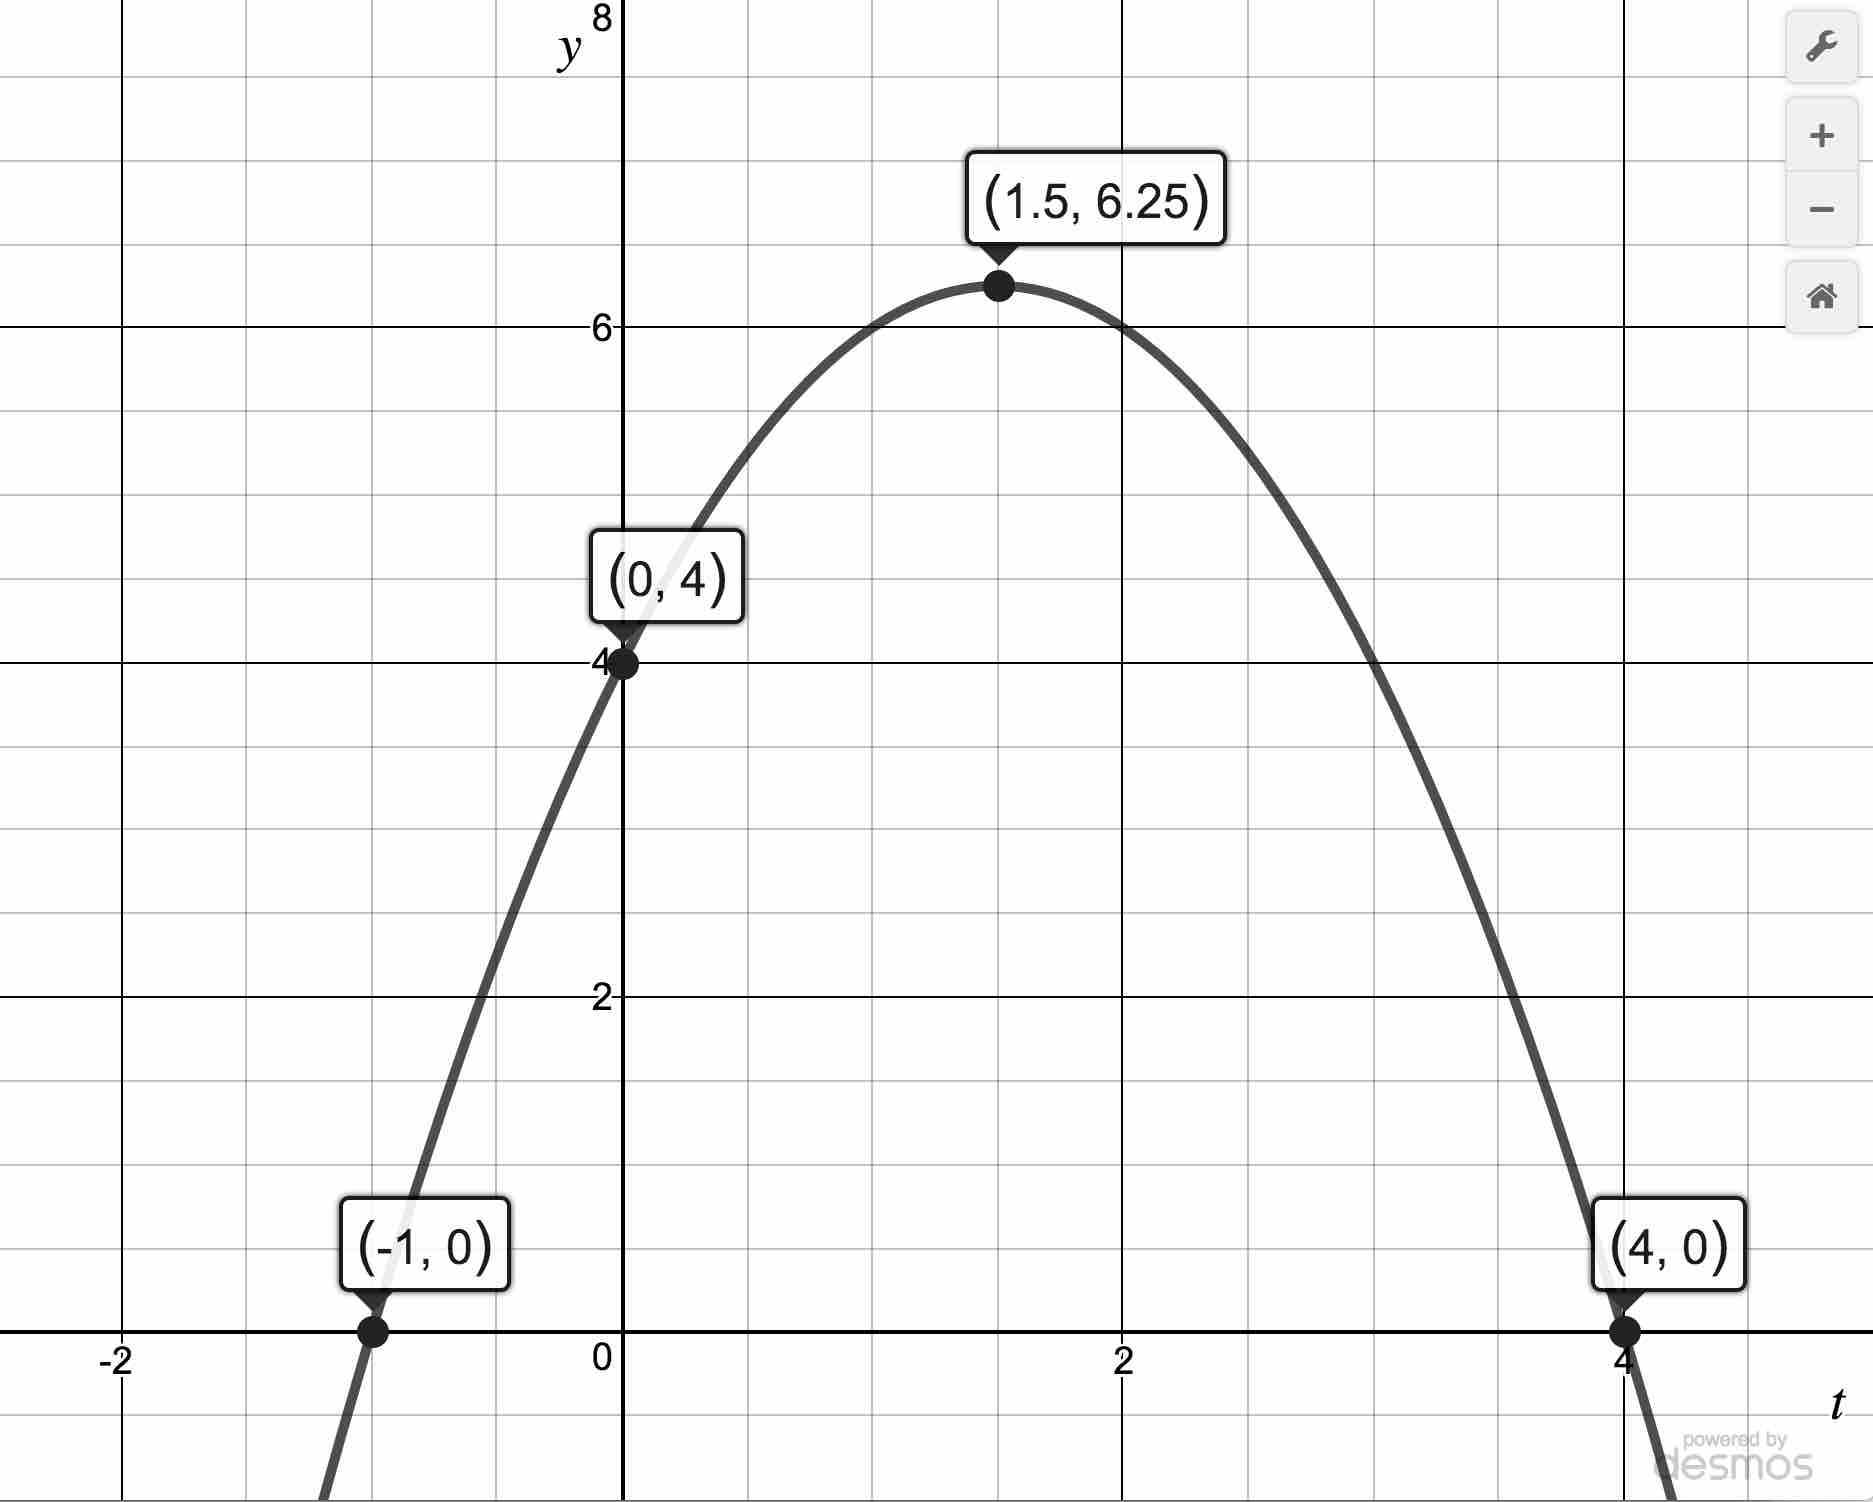
\includegraphics[width=3in]{./FunctionsandtheirRepresentationsGraphics/ParabolaGraph.jpg}

&

\begin{mfpic}[19]{-3}{5}{-2}{7}
\axes
\tlabel[cc](5,-0.5){\scriptsize $t$}
\tlabel[cc](0.5,7){\scriptsize $y$}
\xmarks{-2 step 1 until 4 }
\ymarks{-1 step 1 until 6}
\tlpointsep{5pt}
\scriptsize
\tlabel[cc](-1.75,0.5){$(-1,0)$}
\tlabel[cc](-0.75,4){$(0,4)$}
\tlabel[cc](2.75,6){$(2,6)$}
\tlabel[cc](4.5,0.5){$(4,0)$}
\tlabel[cc](1.5,6.75){$(1.5,6.25)$}

\axislabels {x}{{$-2 \hspace{7pt}$} -2,{$-1 \hspace{7pt}$} -1, {$1$} 1, {$2$} 2, {$3$} 3, {$4$} 4}
\axislabels {y}{{$-1$} -1, {$1$} 1, {$2$} 2, {$3$} 3, {$5$} 5, {$6$} 6}
\normalsize
\penwd{1.5pt}
\arrow \reverse \arrow \function{-1.3,4.3,0.1}{4+3x-x**2}
\point[4pt]{(-1,0), (0,4), (1.5, 6.25), (2,6), (4,0)}
\end{mfpic}  \\

\end{tabular}

\end{center}

\vspace*{-.5in} \qed

\end{ex}

Our last example of the section uses the interplay between algebraic and graphical representations of a function to solve a real-world problem.

\begin{ex} \label{volumeex1}    The United States Postal Service mandates that when shipping parcels using `Parcel Select' service,  the sum of the length (the longest dimension) and the girth (the distance around the thickest part of the parcel perpendicular to the length) must not exceed 130 inches.\footnote{See \href{http://pe.usps.com/text/qsg300/Q201e.htm}{\underline{here}}.}  Suppose we wish to ship a rectangular box whose girth forms a square measuring $x$ inches per side as shown below.

\begin{center}

\begin{mfpic}[10]{-6}{12}{-1}{17}
\polyline{(0,0),(-4,3)}
\polyline{(-4,3), (-4,8)}
\polyline{(-4,8),(0,5)}
\polyline{(0,5),(0,0)}
\polyline{(0,0),(12,9)}
\polyline{(0,5),(12,14)}
\polyline{(-4,8),(8,17)}
\polyline{(8,17),(12,14)}
\polyline{(12,14),(12,9)}%6
\arrow \reverse \arrow \polyline{(0.5,-0.125),(12,8.5)}
\tlabel[cc](9,4){length}
\arrow \reverse \arrow \polyline{(-4, 2.5), (-0.5,-0.125)}
\tlabel[cc](-3,0.5){ $x$}
\arrow \reverse \arrow \polyline{(-4.5, 3), (-4.5,8)}
\tlabel[cc](-5,5){$x$}
\end{mfpic}

\end{center}

It turns out\footnote{We'll skip the explanation for now because we want to focus on just the different representations of the function. Rest assured, you'll be asked to construct this very model in Exercise \ref{girthbox1} in Section \ref{GraphsofPolynomials}.} that the volume of a box, $V(x)$, measured in cubic inches,  whose length plus girth is exactly 130 inches is given by the formula: $V(x) = x^2 (130-4x)$ for $0 < x \leq 26$.

\pagebreak

\begin{enumerate}

\item  Find and interpret $V(5)$.

\item  Make a table of values and use these along with a graphing utility to graph $y = V(x)$.

\item  What is the largest volume box that can be shipped?  What value of $x$ maximizes the volume?  Round your answers to two decimal places.

\end{enumerate}
{\bf Solution.}

\begin{enumerate}

\item To find $V(5)$, we substitute $x=5$ into the expression $V(x)$:  $V(5) = (5)^2 (130-4(5)) = 25(110) = 2750$.   Our result means that when the length and width of the square  measure $5$ inches, the volume of the resulting box is $2750$ cubic inches.\footnote{Note that we have $V(5)$ and $25(110)$ in the same string of equality. The first set of parentheses is function notation and directs us to substitute $5$ for $x$ in the expression $V(x)$ while the second indicates multiplying $25$ by $110$. Context is key!}

\item The domain of $V$ is specified by the inequality  $0 < x \leq 26$, so we can begin graphing $V$ by sampling  $V$ at finitely many $x$-values in this interval to help us get a sense of the range of $V$. This, in turn, will help us determine an adequate viewing window on our graphing utility when the time comes.

It seems natural to start with what's happening near $x = 0$.  Even though the expression $x^2 (130-4x)$  is defined when we substitute $x = 0$ (it reduces very quickly to $0$), it would be incorrect to state $V(0) = 0$ because $x = 0$ is not in the domain of $V$.  However,  there is nothing stopping us from evaluating $V(x)$ at values $x$ `very close' to $x = 0$.  A table of such values is given below. \[ \begin{array}{||l|l||} \hline 
        x & V(x) \\ \hline
      0.1 & 1.296 \\ \hline
     0.01 & 0.012996 \\ \hline
    0.001 & 0.000129996 \\ \hline
10^{-23} & \approx 1.3 \times 10^{-44} \\ \hline

\end{array} \] There is no such thing as a  `smallest' positive number,\footnote{If $p$ is any positive real number, $0 < 0.5 p < p$, so we can always find a smaller positive real number.}  so we will have points on the graph of $V$ to the right of $x = 0$ leading to the point $(0,0)$.  We indicate this behavior by putting a hole at $(0,0)$.\footnote{What's really needed here is the precise definition of `closeness' discussed in Calculus.  This hand-waving will do for now.}

Moving forward, we start with $x = 5$ and sample $V$ at steps of $5$ in its domain.  Our goal is to graph $y = V(x)$, so we plot our points $(x, V(x))$  using  the domain as a guide to help us set the horizontal bounds (i.e., the bounds on $x$) and the sample values from the range to help us set the vertical bounds (i.e., the bounds on $y$).   The right endpoint, $x = 26$, is included in the domain $0 < x \leq 26$ so we finish the graph by plotting the point $(26, V(26)) = (26,17576)$.  At the top of the next page on the left is the table of data and on the right is a graph produced with some help from \href{https://www.desmos.com/}{\underline{desmos}}.
  
\begin{tabular}{m{1.9 in}m{4in}}

$\begin{array}{|r||c|c|}  \hline

  x & V(x) & (x,V(x)) \\ \hline
  
\approx 0 & \approx 0  & \text{hole at $(0,0)$} \\  \hline
 5 & 2750 & (5, 2750) \\  \hline
 10 & 9000 & (10, 9000) \\  \hline
 15 & 15, \! 750 & ( 15, 15, \! 750) \\  \hline
  20 & 20, \! 000 & ( 20 , 20, \! 000) \\  \hline
  25 & 18, \! 750 & ( 25, 18, \! 750) \\  \hline
  26 & 17, \! 576 &  (26,17, \! 576) \\ \hline
\end{array}$

&

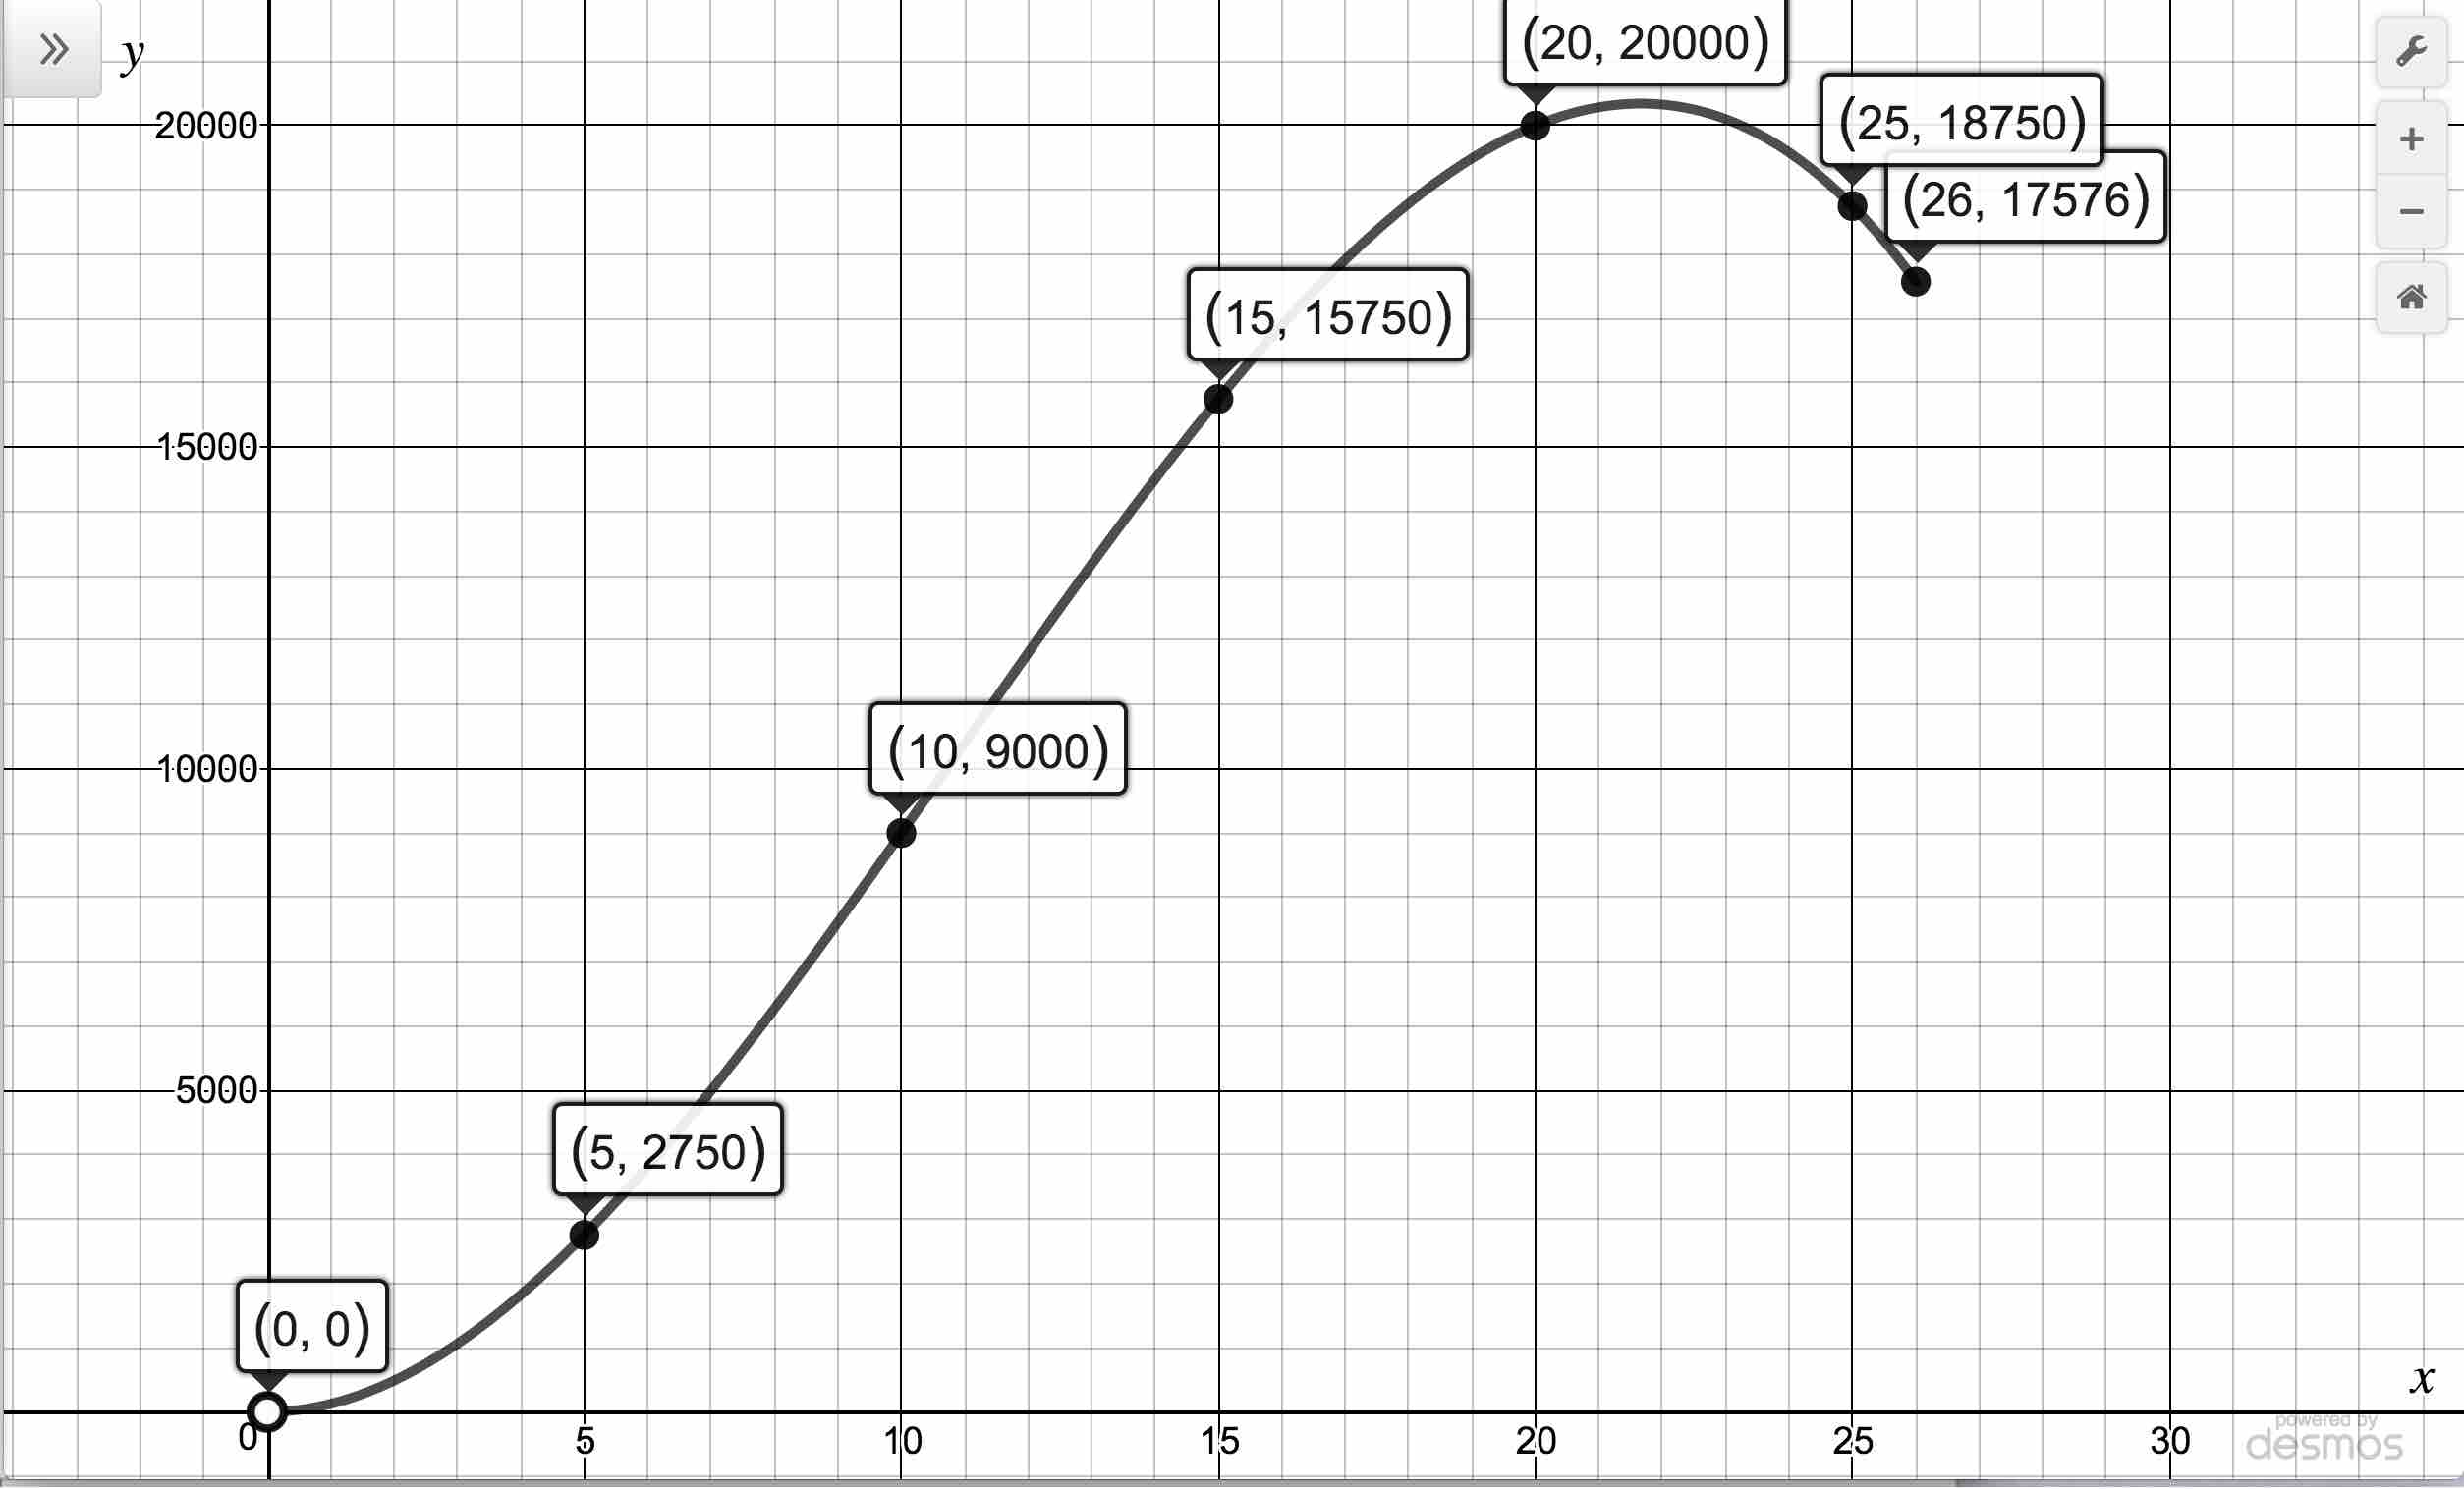
\includegraphics[width=4in]{./FunctionsandtheirRepresentationsGraphics/VolumeEx01.jpg}  \\

\centerline{Sampling $V$}

&

\centerline{The graph of $y = V(x)$}

\end{tabular}


\item  The largest volume in this case refers to the maximum of $V$.  The biggest $y$-value in our table of data is $20, \! 000$ cubic inches which occurs at $x = 20$ inches, but the graph produced by the graphing utility indicates that there are points on the graph of $V$ with $y$-values (hence $V(x)$ values) greater than $20, \! 000$.  Indeed, the graph continues to rise to the right of $x = 20$ and the graphing utility reports the maximum $y$-value to be $y \approx 20, \! 342.593$ when $x \approx 21.667$.  Rounding to two decimal places, we find the maximum volume obtainable under these conditions is about $20, \! 342.59$ cubic inches which occurs when the length and width of the square side of the box are approximately $21.67$ inches.\footnote{We could also find the length of the box in this case as well.  The sum of length and girth is 130 inches so the length is 130 minus the girth, or $130 - 4x \approx 130 - 4(21.67) = 43.32$ inches.}  

\begin{center}

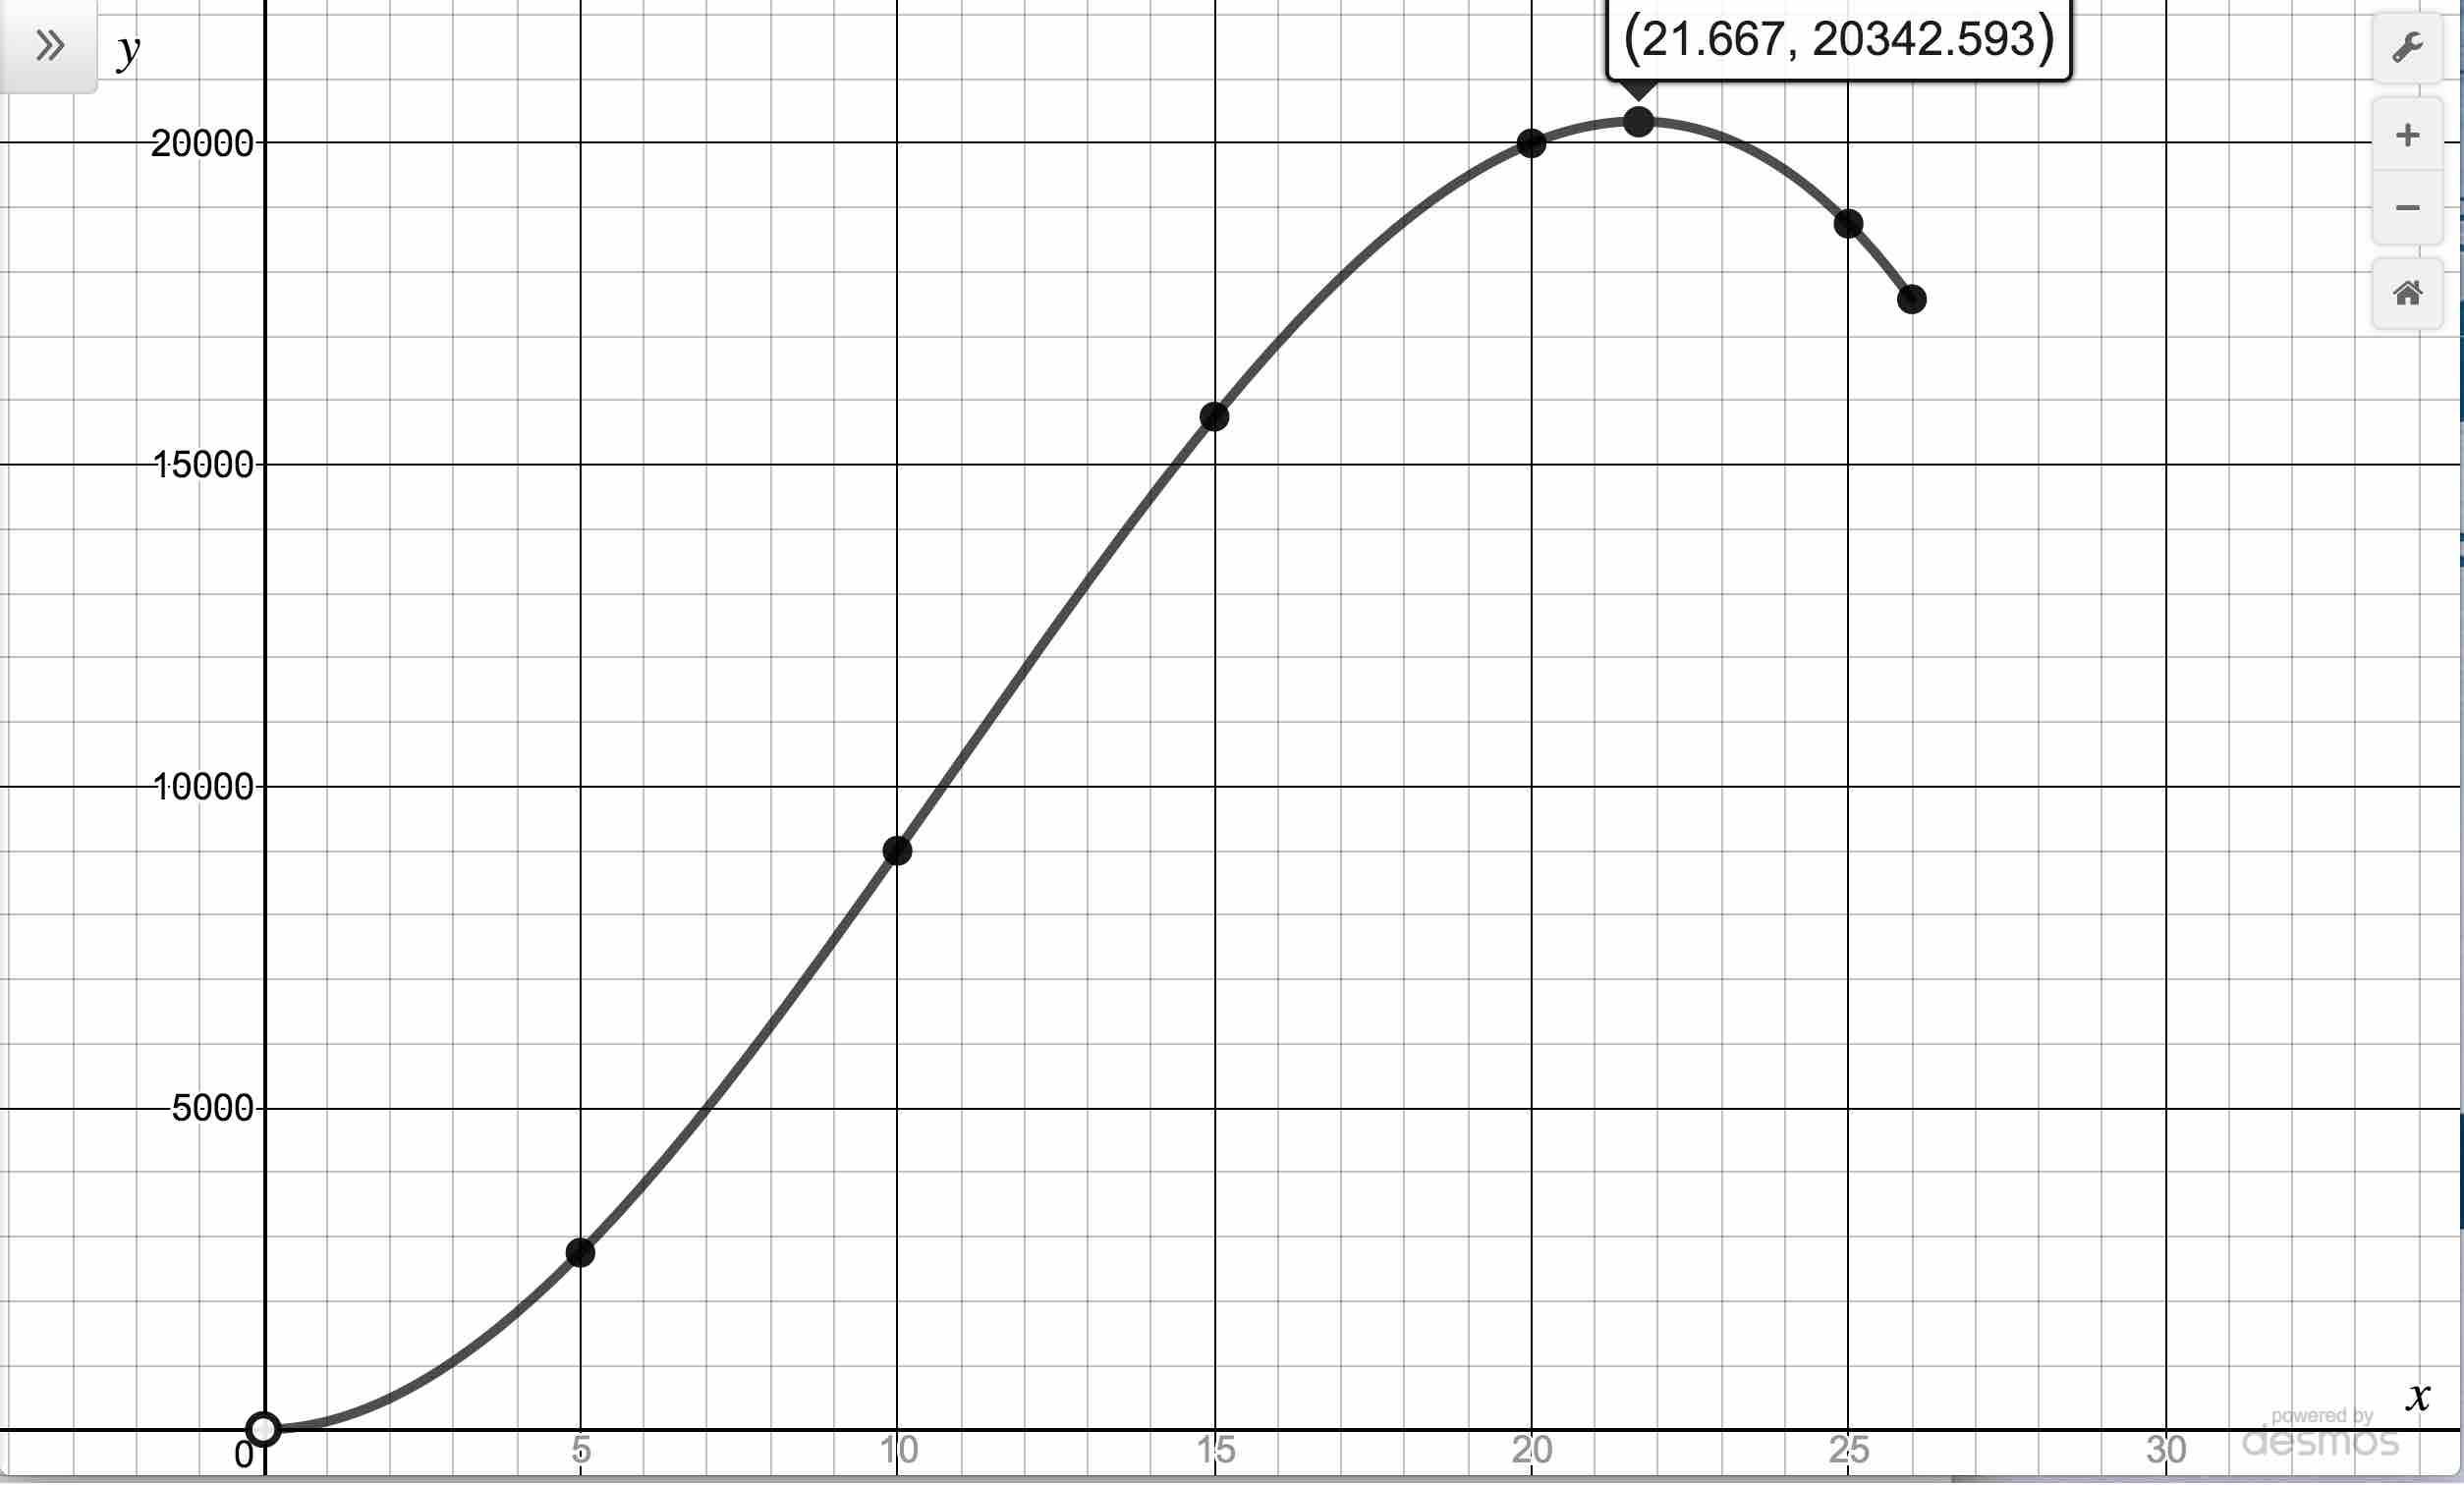
\includegraphics[width=4in]{./FunctionsandtheirRepresentationsGraphics/VolumeEx02.jpg} 

Finding the maximum volume using the graph of $y = V(x)$.

\end{center}

\pagebreak

It is worth noting that while the function $V$ has a maximum, it did not have a minimum.  Even though $V(x)>0$ for all $x$ in its domain,\footnote{said differently, the values of $V(x)$ are \textbf{bounded below} by $0$.} the presence of the hole at $(0,0)$ means that $0$ is not in the range of $V$.  Hence, based on our model, we can never make a box with a  `smallest' volume.\footnote{How realistic is this?}  \qed

\end{enumerate}
\end{ex}

\medskip

Example \ref{volumeex1} typifies the interplay between Algebra and Geometry which lies ahead.  Both the algebraic description of  $V$: $V(x) = x^2 (130 - 4x)$ for $0 < x \leq 26$, and the graph of $y=V(x)$ were useful in describing aspects of the physical situation at hand.  Wherever possible, we'll use the algebraic representations of functions to \textit{analytically} produce \textit{exact} answers to certain problems and use the graphical descriptions to check the reasonableness of our answers. 

\medskip

That being said, we'll also encounter problems which we simply \textit{cannot} answer analytically (such as determining the maximum volume in the previous example), so we will be forced to resort to using technology (specifically graphing technology) in order to find \textit{approximate} solutions.  The most important thing to keep in mind is that while technology may \textit{suggest} a result, it is ultimately Mathematics that \textit{proves} it. 

\medskip

We close this section with a summary of the different ways to represent functions.

\bigskip

\colorbox{ResultColor}{\bbm

\centerline{\textbf{Ways to Represent a Function}} \label{waystorepresentfunctionsbox}

\smallskip

Suppose $f$ is a function with domain $A$.  Then $f$ can be represented:

\begin{itemize}

\item  verbally; that is, by describing how the inputs are matched with their outputs.

\item using a mapping diagram.

\item  as a set of ordered pairs of the form $(\text{input}, \text{output})$:  $\{ (a, f(a)) \, | \, a \in A \}$.

\end{itemize}

If $f$ is a function whose domain and range are subsets of real numbers, then $f$ can be represented:

\begin{itemize}

\item  algebraically as a formula for $f(a)$.

\item  graphically by plotting the points $\{ (a, f(a))  \, | \, a \in A \}$ in the plane.

\end{itemize}

Note: An important consequence of the last bulleted item is that the point $(a, b)$ is on the graph of $y = f(x)$ if and only if $f(a) = b.$\label{FundamentalGraphingPrinciple}

\ebm}

\newpage

\subsection{Exercises}
In Exercises \ref{mappingfirst} - \ref{mappinglast}, determine whether or not the mapping diagram represents a function. Explain your reasoning. If the mapping does represent a function, state the domain, range, and represent the function as a set of ordered pairs.

\begin{multicols}{2}

\begin{enumerate}


\item  \label{mappingfirst} 

$~$

\begin{mfpic}[19]{-5}{5}{-5}{6}
\tlabel[cc](-4.25,5){Tennant}
\tlabel[cc](-4.25,3){Smith}
\tlabel[cc](-4.25,1){Calpadi}
\tlabel[cc](0,6){$M$}
\tlabel[cc](3.5,5){Eleven}
\tlabel[cc](3.5,3){Twelve}
\tlabel[cc](3.5,1){Thirteen}
\tlabel[cc](3.5,-1){Fourteen}
\arrow[l 5pt] \polyline{(-2.5, 5), (2.5, 5)}
\arrow[l 5pt] \polyline{(-2.5, 5), (2.5, 3)}
\arrow[l 5pt] \polyline{(-2.5, 3), (2.5, 1)}
\arrow[l 5pt] \polyline{(-2.5, 1), (2.5, -1)}
\end{mfpic} 



\item  \label{mappinglast} 

$~$

\begin{mfpic}[19]{-5}{5}{-5}{6}
\tlabel[cc](-4.25,5){Hartnell}
\tlabel[cc](-4.25,3){Cushing}
\tlabel[cc](-4.25,1){Hurndall}
\tlabel[cc](-4.25,-1){Troughton}
\tlabel[cc](0,6){$C$}
\tlabel[cc](3.5,5){One}
\tlabel[cc](3.5,3){Two}
\tlabel[cc](3.5,1){Three}
\arrow[l 5pt] \polyline{(-2.5, 5), (2.5, 5)}
\arrow[l 5pt] \polyline{(-2.5, 3), (2.5, 5)}
\arrow[l 5pt] \polyline{(-2.5, 1), (2.5, 5)}
\arrow[l 5pt] \polyline{(-2.5, -1), (2.5, 3)}
\end{mfpic}

\setcounter{HW}{\value{enumi}}

\end{enumerate}

\end{multicols}

In Exercises \ref{tablefirst} - \ref{tablelast}, determine whether or not the data in the given table represents $y$ as a function of $x$.  Explain your reasoning.  If the mapping does represent a function, state the domain, range, and represent the function as a set of ordered pairs.

\begin{multicols}{2}

\begin{enumerate}

\setcounter{enumi}{\value{HW}}

\item  \label{tablefirst} 

\[\begin{array}{|r||r|}  \hline

$x$  & \hphantom{\text{$-$}} $y$  \\ \hline
 -3 &  3 \\  \hline
 -2 & 2  \\  \hline
  -1 &  1  \\  \hline
 0 &  0 \\  \hline
 1 & 1  \\  \hline
 2 &  2 \\  \hline
 3 & 3  \\  \hline

\end{array}\]

\item \label{tablelast}

\[\begin{array}{|r||r|}  \hline

\hphantom{\text{$-$}} $x$  &$y$  \\ \hline

 0 & 0 \\  \hline
 1 & 1  \\  \hline
 1 & -1  \\  \hline
 2 &  2 \\  \hline
 2 & -2  \\  \hline
 3 &  3 \\  \hline
 3 & -3  \\  \hline

\end{array}\]

\setcounter{HW}{\value{enumi}}

\end{enumerate}

\end{multicols}

\begin{enumerate}

\setcounter{enumi}{\value{HW}}

\item    Suppose $W$ is the set of words in the English language and we set up a mapping from $W$ into the set of natural numbers $\mathbb{N}$ as follows: $\text{word} \rightarrow \text{number of letters in the word}$.  Explain why this mapping is a function.  What would you need to know to determine the range of the function?

\item  Suppose $L$ is the set of last names of all the people who have served or are currently serving as the President of the United States.   Consider the mapping from $L$ into $\mathbb{N}$ as follows:  $\text{last name} \rightarrow \text{number of their presidency}$.  For example,  $\text{Washington} \rightarrow 1$ and $\text{Obama} \rightarrow 44$.  Is this mapping a function?  What if we use full names instead of just last names? (\textbf{HINT:}  Research Grover Cleveland.)

\item  Under what conditions would the time of day be a function of the outdoor temperature?

\setcounter{HW}{\value{enumi}}

\end{enumerate}


For the functions $f$ described in Exercises \ref{buildfunctionfirst} - \ref{buildfunctionlast}, find $f(2)$ and find and simplify an expression for $f(x)$ that takes a real number $x$ and performs the following three steps in the order given: 


\begin{enumerate}
\setcounter{enumi}{\value{HW}}

\item  (1) multiply by 2; (2) add 3; (3) divide by 4. \label{buildfunctionfirst}

\item  (1) add 3; (2) multiply by 2; (3) divide by 4. 

\item (1) divide by 4; (2) add 3; (3) multiply by 2.

\item (1) multiply by 2; (2) add 3; (3) take the square root.

\item  (1) add 3; (2) multiply by 2; (3) take the square root.

\item  (1) add 3; (2) take the square root; (3) multiply by 2.  \label{buildfunctionlast}

\setcounter{HW}{\value{enumi}}
\end{enumerate}


In Exercises \ref{funcnotationbasicfirst} - \ref{funcnotationbasiclast}, use the given function $f$ to find and simplify the following:

\begin{multicols}{3}
\begin{itemize}
\item $f(3)$
\item $f(-1)$
\item $f\left(\frac{3}{2} \right)$
\end{itemize}
\end{multicols}

\begin{multicols}{3}
\begin{itemize}
\item  $f(4x)$
\item $4f(x)$
\item $f(-x)$
\end{itemize}
\end{multicols}

\begin{multicols}{3}
\begin{itemize}
\item  $f(x-4)$
\item $f(x) - 4$
\item  $f\left(x^2\right)$
\end{itemize}
\end{multicols}

\begin{multicols}{2}
\begin{enumerate}
\setcounter{enumi}{\value{HW}}

\item  $f(x) = 2x+1$ \label{funcnotationbasicfirst} 
\item  $f(x) = 3 - 4x$

\setcounter{HW}{\value{enumi}}
\end{enumerate}
\end{multicols}

\begin{multicols}{2}
\begin{enumerate}
\setcounter{enumi}{\value{HW}}

\item $f(x) = 2 - x^2$
\item $f(x) = x^2 - 3x + 2$

\setcounter{HW}{\value{enumi}}
\end{enumerate}
\end{multicols}


\begin{multicols}{2}
\begin{enumerate}
\setcounter{enumi}{\value{HW}}

\item $f(x) = 6$
\item $f(x) = 0$ \label{funcnotationbasiclast}

\setcounter{HW}{\value{enumi}}
\end{enumerate}
\end{multicols}

In Exercises \ref{secondfuncnotationbasicfirst} - \ref{secondfuncnotationbasiclast}, use the given function $f$ to find and simplify the following:

\begin{multicols}{3}
\begin{itemize}

\item  $f(2)$
\item  $f(-2)$
\item  $f(2a)$

\end{itemize}
\end{multicols}

\begin{multicols}{3}
\begin{itemize}

\item  $2 f(a)$
\item $f(a+2)$
\item $f(a) + f(2)$

\end{itemize}
\end{multicols}

\begin{multicols}{3}
\begin{itemize}

\item  $f \left( \dfrac{2}{a} \right)$
\item $\dfrac{f(a)}{2}$
\item  $f(a + h)$

\end{itemize}
\end{multicols}


\begin{multicols}{2}
\begin{enumerate}
\setcounter{enumi}{\value{HW}}

\item $f(x) = 2x-5$ \label{secondfuncnotationbasicfirst}
\item $f(t) = 5-2t$

\setcounter{HW}{\value{enumi}}
\end{enumerate}
\end{multicols}

\begin{multicols}{2}
\begin{enumerate}
\setcounter{enumi}{\value{HW}}

\item $f(w) = 2w^2 - 1$
\item $f(q) = 3q^2+3q-2$

\setcounter{HW}{\value{enumi}}
\end{enumerate}
\end{multicols}
 
\begin{multicols}{2}
\begin{enumerate}
\setcounter{enumi}{\value{HW}}


\item $f(r) = 117$
\item $f(z) = \dfrac{z}{2}$  \label{secondfuncnotationbasiclast}

\setcounter{HW}{\value{enumi}}
\end{enumerate}
\end{multicols}


\newpage


In Exercises \ref{findzerofuncfirst} - \ref{findzerofunclast}, use the given function $f$ to find $f(0)$ and solve $f(x) = 0$

\begin{multicols}{2}
\begin{enumerate}
\setcounter{enumi}{\value{HW}}

\item $f(x) = 2x - 1$ \label{findzerofuncfirst}
\item $f(x) = 3 - \frac{2}{5} x$

\setcounter{HW}{\value{enumi}}
\end{enumerate}
\end{multicols}

\begin{multicols}{2}
\begin{enumerate}
\setcounter{enumi}{\value{HW}}

\item $f(x) = 2x^2 - 6$
\item $f(x) = x^2 - x - 12$ \label{findzerofunclast}

\setcounter{HW}{\value{enumi}}
\end{enumerate}
\end{multicols}


In Exercises \ref{equfunctionfirst} - \ref{equfunctionlast}, determine whether or not the equation represents $y$ as a function of $x$.  



\begin{multicols}{3}
\begin{enumerate}
\setcounter{enumi}{\value{HW}}

\item $y = x^{3} - x$ \label{equfunctionfirst}
\item $y = \sqrt{x - 2}$
\item $x^{3}y = -4$ 
\setcounter{HW}{\value{enumi}}
\end{enumerate}
\end{multicols}

\begin{multicols}{3}
\begin{enumerate}
\setcounter{enumi}{\value{HW}}

\item $x^{2} - y^{2} = 1$
\item $y = \dfrac{x}{x^{2} - 9}$
\item $x = -6$

\setcounter{HW}{\value{enumi}}
\end{enumerate}
\end{multicols}

\begin{multicols}{3}
\begin{enumerate}
\setcounter{enumi}{\value{HW}}

\item  $x = y^2 + 4$

\item $y = x^2 + 4$
\item $x^2 + y^2 = 4$

\setcounter{HW}{\value{enumi}}
\end{enumerate}
\end{multicols}

\begin{multicols}{3}
\begin{enumerate}
\setcounter{enumi}{\value{HW}}


\item $y = \sqrt{4-x^2}$
\item $x^2 - y^2 = 4$
\item $x^3 + y^3 = 4$


\setcounter{HW}{\value{enumi}}
\end{enumerate}
\end{multicols}

\begin{multicols}{3}
\begin{enumerate}
\setcounter{enumi}{\value{HW}}

\item $2x + 3y = 4$
\item $2xy = 4$
\item $x^2 = y^2$ \label{equfunctionlast}

\setcounter{HW}{\value{enumi}}
\end{enumerate}
\end{multicols}





Exercises \ref{setfunctionfirst} - \ref{setfunctionlast} give a set of points in the $xy$-plane.    Determine if $y$ is a function of $x$.  If so, state the domain and range.

\begin{enumerate}

\setcounter{enumi}{\value{HW}}

\item \{$(-3, 9)$, $\;(-2, 4)$, $\;(-1, 1)$, $\;(0, 0)$, $\;(1, 1)$, $\;(2, 4)$, $\;(3, 9)\}$ \label{setfunctionfirst}
\item  $\left\{ (-3,0), (1,6), (2, -3), (4,2), (-5,6), (4, -9), (6,2) \right\}$
\item  $\left\{ (-3,0), (-7,6), (5,5), (6,4), (4,9), (3,0) \right\}$
\item  $\left\{ (1,2), (4,4), (9,6), (16,8), (25,10), (36, 12), \ldots \right\}$
\item \{($x, y) \, | \, x$ is an odd integer, and $y$ is an even integer\}
\item \{$(x, 1) \, | \, x$ is an irrational number\}

\item $\{ (1,0), (2,1), (4,2), (8,3), (16,4), (32, 5), \ldots \}$
\item $\{ \ldots (-3,9), (-2,4), (-1,1), (0,0), (1,1), (2,4), (3,9), \ldots \}$

\setcounter{HW}{\value{enumi}}
\end{enumerate}

\vspace{-0.1in}

\begin{multicols}{2}
\begin{enumerate}
\setcounter{enumi}{\value{HW}}

\item $\{ (-2, y) \, | \, -3 < y < 4\}$
\item  $\{ (x,3) \, | \,  -2 \leq x < 4\}$

\setcounter{HW}{\value{enumi}}
\end{enumerate}
\end{multicols}

\begin{multicols}{2}
\begin{enumerate}
\setcounter{enumi}{\value{HW}}


\item  $\{ \left(x,x^2\right) \, | \, \text{$x$ is a real number} \}$
\item  $\{ \left(x^2,x\right) \, | \, \text{$x$ is a real number} \}$ \label{setfunctionlast}

\setcounter{HW}{\value{enumi}}
\end{enumerate}
\end{multicols}

\begin{enumerate}
\setcounter{enumi}{\value{HW}}

\item  \label{HLTExercise} The Vertical Line Test is a quick way to determine from a graph if the vertical axis variable is a function of the horizontal axis variable. If we are given a graph and asked to determine if the horizontal axis variable is a function of the vertical axis variable, we can use horizontal lines instead of vertical lines to check.  Using Theorem \ref{VLT} as a guide,  formulate a `Horizontal Line Test.'  (We'll refer back to this exercise in Section \ref{InverseFunctions}.)

\setcounter{HW}{\value{enumi}}
\end{enumerate}

\newpage


In Exercises \ref{graphfunctionfirstxy} - \ref{graphfunctionlastxy}, determine whether or not the graph suggests $y$ is a function of $x$.  For the ones which do, state the domain and range. 

\begin{multicols}{2}
\begin{enumerate}
\setcounter{enumi}{\value{HW}}

\item $~$ \vspace{-.1in} \label{graphfunctionfirstxy}

\begin{mfpic}[17]{-5}{2}{-2}{5}
\point[4pt]{(-4, -1), (-3, 0), (-2, 1), (-1, 2), (0, 3), (1, 4)}
\axes
\tlabel[cc](2,-0.5){\scriptsize $x$}
\tlabel[cc](0.5,4.75){\scriptsize $y$}
\xmarks{-4,-3,-2,-1,1}
\ymarks{-1,1,2,3,4}
\tlpointsep{4pt}
\axislabels {x}{{\tiny $-4 \hspace{8pt}$} -4, {\tiny $-3 \hspace{8pt}$} -3, {\tiny $-2 \hspace{8pt}$} -2, {\tiny $-1 \hspace{8pt}$} -1, {\tiny $1$} 1}
\axislabels {y}{{\tiny $-1$} -1, {\tiny $1$} 1, {\tiny $2$} 2, {\tiny $3$} 3, {\tiny $4$} 4}
\end{mfpic}

\vfill
\columnbreak

\item $~$  \label{graphfunctionfirstxy2}

\begin{mfpic}[15]{-5}{2}{-2}{5}
\point[4pt]{(-4, -1), (-3, 0), (-3, 1), (-2, 1), (-1, 2), (0, 3), (1, 4)}
\axes
\tlabel[cc](2,-0.5){\scriptsize $x$}
\tlabel[cc](0.5,4.75){\scriptsize $y$}
\xmarks{-4,-3,-2,-1,1}
\ymarks{-1,1,2,3,4}
\tlpointsep{4pt}
\axislabels {x}{{\tiny $-4 \hspace{6pt}$} -4, {\tiny $-3 \hspace{6pt}$} -3, {\tiny $-2 \hspace{6pt}$} -2, {\tiny $-1 \hspace{6pt}$} -1, {\tiny $1$} 1}
\axislabels {y}{{\tiny $-1$} -1, {\tiny $1$} 1, {\tiny $2$} 2, {\tiny $3$} 3, {\tiny $4$} 4}
\end{mfpic}


\setcounter{HW}{\value{enumi}}
\end{enumerate}
\end{multicols}


\begin{multicols}{2}
\begin{enumerate}
\setcounter{enumi}{\value{HW}}



\item $~$ \label{graphfunctionfirstxy3}

\begin{mfpic}[15]{-3}{3}{-1}{6}
\axes
\tlabel[cc](3,-0.5){\scriptsize $x$}
\tlabel[cc](0.5,5.75){\scriptsize $y$}
\xmarks{-2,-1,1,2}
\ymarks{1,2,3,4,5}
\tlpointsep{4pt}
\axislabels {x}{{\tiny $-2 \hspace{8pt}$} -2, {\tiny $-1 \hspace{8pt}$} -1, {\tiny $1$} 1, {\tiny $2$} 2}
\axislabels {y}{{\tiny $1$} 1, {\tiny $2$} 2, {\tiny $3$} 3, {\tiny $4$} 4, {\tiny $5$} 5}
\penwd{1.25pt}
\arrow \reverse \arrow \function{-2.1, 2.1, 0.1}{x**2+1}
\end{mfpic}

\vfill
\columnbreak

\item $~$  \label{graphfunctionlastxy}

\begin{mfpic}[15]{-4}{4}{-4}{4}
\axes
\tlabel[cc](4,-0.5){\scriptsize $x$}
\tlabel[cc](0.5,3.75){\scriptsize $y$}
\xmarks{-3,-2,-1,1,2,3}
\ymarks{-3,-2,-1,1,2,3}
\tlpointsep{4pt}
\axislabels {x}{{\tiny $-3 \hspace{8pt}$} -3, {\tiny $-2 \hspace{8pt}$} -2, {\tiny $-1 \hspace{8pt}$} -1, {\tiny $1$} 1, {\tiny $2$} 2, {\tiny $3$} 3}
\axislabels {y}{{\tiny $-3$} -3, {\tiny $-2$} -2, {\tiny $-1$} -1, {\tiny $1$} 1, {\tiny $2$} 2, {\tiny $3$} 3}
\penwd{1.25pt}
\arrow \reverse \arrow \parafcn{-2,2,0.1}{(cosh(t),sinh(t))}
\end{mfpic}


\setcounter{HW}{\value{enumi}}
\end{enumerate}
\end{multicols}

\begin{enumerate}
\setcounter{enumi}{\value{HW}}

\item   Determine which, if any, of the graphs in numbers \ref{graphfunctionfirstxy} - \ref{graphfunctionlastxy} represent $x$ as a function of $y$.  For the ones which do, state the domain and range.  (Feel free to use Exercise \ref{HLTExercise}.)

\setcounter{HW}{\value{enumi}}
\end{enumerate}

In Exercises \ref{graphfunctionfirstvw} - \ref{graphfunctionlastvw}, determine whether or not the graph suggests $w$ is a function of $v$ .  For the ones which do, state the domain and range. 


\begin{multicols}{2}
\begin{enumerate}
\setcounter{enumi}{\value{HW}}

\item $~$ \label{graphfunctionfirstvw}  

\begin{mfpic}[15]{-1}{10}{-1}{4}
\axes
\tlabel[cc](10,-0.5){\scriptsize $v$}
\tlabel[cc](0.5,3.75){\scriptsize $w$}
\xmarks{1,2,3,4,5,6,7,8,9}
\ymarks{1,2,3}
\tlpointsep{4pt}
\axislabels {x}{{\tiny $1$} 1, {\tiny $2$} 2, {\tiny $3$} 3, {\tiny $4$} 4, {\tiny $5$} 5, {\tiny $6$} 6, {\tiny $7$} 7, {\tiny $8$} 8, {\tiny $9$} 9}
\axislabels {y}{{\tiny $1$} 1, {\tiny $2$} 2, {\tiny $3$} 3}
\penwd{1.25pt}
\arrow \function{2, 10, 0.1}{sqrt(x - 2)}
\point[4pt]{(2,0)}
\end{mfpic}

\vfill
\columnbreak

\item $~$ \label{graphfunctionfirstvw2} 

\begin{mfpic}[15]{-5}{5}{-1}{5}
\axes
\tlabel[cc](5,-0.5){\scriptsize $v$}
\tlabel[cc](0.5,4.75){\scriptsize $w$}
\xmarks{-4,-3,-2,-1,1,2,3,4}
\ymarks{1,2,3,4}
\tlpointsep{4pt}
\axislabels {x}{{\tiny $-4 \hspace{8pt}$} -4, {\tiny $-3 \hspace{8pt}$} -3, {\tiny $-2 \hspace{8pt}$} -2, {\tiny $-1 \hspace{8pt}$} -1, {\tiny $1$} 1, {\tiny $2$} 2, {\tiny $3$} 3, {\tiny $4$} 4}
\axislabels {y}{{\tiny $1$} 1, {\tiny $2$} 2, {\tiny $3$} 3, {\tiny $4$} 4}
\penwd{1.25pt}
\arrow \reverse \arrow \function{-5, 5, 0.1}{4/(x**2 + 1)}
\end{mfpic}


\setcounter{HW}{\value{enumi}}
\end{enumerate}
\end{multicols}

\newpage

\begin{multicols}{2}
\begin{enumerate}
\setcounter{enumi}{\value{HW}}

\item $~$  \label{graphfunctionfirstvw3} 

\begin{mfpic}[15]{-4.5}{5.5}{-4}{3}
\axes
%\fillcolor[gray]{.7}
%\gfill \rect{(-3.97, -2.97), (4.97, 1.97)}
%\dashed \polyline{(-4, 2), (5, 2)}
%\dashed \polyline{(5, 2), (5, -3)}
%\dashed \polyline{(5, -3), (-4, -3)}
\tlabel[cc](5.5,-0.5){\scriptsize $v$}
\tlabel[cc](0.5,2.75){\scriptsize $w$}
\xmarks{-4,-3,-2,-1,1,2,3,4,5}
\ymarks{-3,-2,-1,1,2}
\tlpointsep{4pt}
\axislabels {x}{{\tiny $-4 \hspace{8pt}$} -4,  {\tiny $-2 \hspace{8pt}$} -2, {\tiny $-1 \hspace{8pt}$} -1, {\tiny $1$} 1, {\tiny $2$} 2, {\tiny $4$} 4, {\tiny $5$} 5}
\axislabels {y}{ {\tiny $-2$} -2, {\tiny $-1$} -1, {\tiny $1$} 1}
\penwd{1.25pt}
\polyline{(-3, -3), (-3, 2), (3,2), (3,-3), (-3,-3)}
\end{mfpic}



\item $~$ \label{graphfunctionlastvw}

\begin{mfpic}[15]{-6}{4}{-2.5}{4.5}
\axes
\tlabel[cc](4,-0.5){\scriptsize $v$}
\tlabel[cc](0.5,4.75){\scriptsize $w$}
\xmarks{-5 step 1 until 3}
\ymarks{-2 step 1 until 4}
\tlpointsep{4pt}
\axislabels {x}{{\tiny $-5 \hspace{8pt}$} -5, {\tiny $-4 \hspace{8pt}$} -4, {\tiny $-3 \hspace{8pt}$} -3, {\tiny $-2 \hspace{8pt}$} -2, {\tiny $-1 \hspace{8pt}$} -1, {\tiny $1$} 1, {\tiny $2$} 2, {\tiny $3$} 3}
\axislabels {y}{{\tiny $-2$} -2, {\tiny $-1$} -1, {\tiny $1$} 1, {\tiny $2$} 2, {\tiny $3$} 3, {\tiny $4$} 4}
\penwd{1.25pt}
\function{-5,-1,0.1}{-5 - 6*x - x**2}
\function{-1,3,0.1}{x/4 - 7/4}
\point[4pt]{(-5, 0), (-1, 0)}
\pointfillfalse
\point[4pt]{(-3,4), (-1,-2), (3,-1)}
\end{mfpic}


\setcounter{HW}{\value{enumi}}
\end{enumerate}
\end{multicols}

\begin{enumerate}
\setcounter{enumi}{\value{HW}}

\item  Determine which, if any, of the graphs in numbers \ref{graphfunctionfirstvw} - \ref{graphfunctionlastvw} represent $v$ as a function of $w$.   For the ones which do, state the domain and range.  (Feel free to use Exercise \ref{HLTExercise}.)

\setcounter{HW}{\value{enumi}}
\end{enumerate}

In Exercises \ref{graphfunctionfirsttT} - \ref{graphfunctionlasttT}, determine whether or not the graph suggests $T$ is a function of $t$.   For the ones which do, state the domain and range. 


\begin{multicols}{2}
\begin{enumerate}
\setcounter{enumi}{\value{HW}}

\item  $~$ \label{graphfunctionfirsttT}

\begin{mfpic}[8]{-4}{4}{-6}{10}

\axes
\tlabel[cc](4,-0.5){\scriptsize $t$}
\tlabel[cc](0.5,10){\scriptsize $T$}
\xmarks{-3,-2,-1,1,2,3}
\ymarks{-5,-4,-3,-2,-1,1,2,3,4,5,6,7,8,9}
\tlpointsep{4pt}
\axislabels {x}{{\tiny $-3 \hspace{6pt}$} -3,{\tiny $-2 \hspace{6pt}$} -2, {\tiny $-1 \hspace{6pt}$} -1, {\tiny $1$} 1, {\tiny $2$} 2, {\tiny $3$} 3}
\axislabels {y}{{\tiny $-5$} -5, {\tiny $-4$} -4, {\tiny $-3$} -3, {\tiny $-2$} -2, {\tiny $-1$} -1, {\tiny $1$} 1, {\tiny $2$} 2, {\tiny $3$} 3, {\tiny $4$} 4, {\tiny $5$} 5, {\tiny $6$} 6, {\tiny $7$} 7, {\tiny $8$} 8, {\tiny $9$} 9}
\penwd{1.25pt}
\arrow \function{-2,4.5,0.1}{x**2 - 2*x - 2}
\point[4pt]{(-2,6), (1,-3) }
\end{mfpic}

\vfill
\columnbreak

\item  $~$  \label{graphfunctionfirsttT2}

\begin{mfpic}[10]{-6}{6}{-6}{6}
\axes
\tlabel[cc](6,-0.5){\scriptsize $t$}
\tlabel[cc](0.5,6){\scriptsize $T$}
\xmarks{-5,-4,-3,-2,-1,1,2,3,4,5}
\ymarks{-5,-4,-3,-2,-1,1,2,3,4,5}
\tlpointsep{4pt}
\axislabels {x}{{\tiny $-5 \hspace{6pt}$} -5,{\tiny $-4 \hspace{6pt}$} -4,{\tiny $-3 \hspace{6pt}$} -3,{\tiny $-2 \hspace{6pt}$} -2, {\tiny $-1 \hspace{6pt}$} -1, {\tiny $1$} 1, {\tiny $2$} 2, {\tiny $3$} 3, {\tiny $4$} 4, {\tiny $5$} 5}
\penwd{1.25pt}
\plrfcn{0,180,5}{5*sind 3t}
\end{mfpic} 


\setcounter{HW}{\value{enumi}}
\end{enumerate}
\end{multicols}

\begin{multicols}{2}
\begin{enumerate}
\setcounter{enumi}{\value{HW}}

\item  $~$  \label{graphfunctionfirsttT3}

\begin{mfpic}[10]{-6}{6}{-6}{6}
\axes
\tlabel[cc](6,-0.5){\scriptsize $t$}
\tlabel[cc](0.5,6){\scriptsize $T$}
\xmarks{-5,-4,-3,-2,-1,1,2,3,4,5}
\ymarks{-5,-4,-3,-2,-1,1,2,3,4,5}
\tlpointsep{4pt}
\axislabels {x}{{\tiny $-5 \hspace{6pt}$} -5,{\tiny $-4 \hspace{6pt}$} -4,{\tiny $-3 \hspace{6pt}$} -3,{\tiny $-2 \hspace{6pt}$} -2, {\tiny $-1 \hspace{6pt}$} -1, {\tiny $1$} 1, {\tiny $2$} 2, {\tiny $3$} 3, {\tiny $4$} 4, {\tiny $5$} 5}
\axislabels {y}{{\tiny $-5$} -5,{\tiny $-4$} -4,{\tiny $-3$} -3, {\tiny $-2$} -2, {\tiny $-1$} -1, {\tiny $1$} 1, {\tiny $2$} 2, {\tiny $3$} 3, {\tiny $4$} 4, {\tiny $5$} 5}
\penwd{1.25pt}
\function{-5,4,0.1}{0.0502*(x**3) - 0.0344*(x**2) - 0.2010*x + 2.138}
\pointfillfalse
\point[4pt]{(-5,-4),(4,4)}

\end{mfpic} 

\vfill
\columnbreak

\item  $~$ \label{graphfunctionlasttT}

\begin{mfpic}[10]{-2}{7}{-6}{6}
\axes
\tlabel[cc](7,-0.5){\scriptsize $t$}
\tlabel[cc](0.5,6){\scriptsize $T$}
\xmarks{-1,1,2,3,4,5,6}
\ymarks{-5,-4,-3,-2,-1,1,2,3,4,5}
\tlpointsep{4pt}
\axislabels {x}{{\tiny $-1 \hspace{6pt}$} -1, {\tiny $1$} 1, {\tiny $2$} 2, {\tiny $3$} 3, {\tiny $4$} 4, {\tiny $5$} 5, {\tiny $6$} 6}
\axislabels {y}{{\tiny $-5$} -5,{\tiny $-4$} -4,{\tiny $-3$} -3, {\tiny $-2$} -2, {\tiny $-1$} -1, {\tiny $1$} 1, {\tiny $2$} 2, {\tiny $3$} 3, {\tiny $4$} 4, {\tiny $5$} 5}
\penwd{1.25pt}
\polyline{(0,-1), (3,-4)}
\polyline{(3,1), (4,4), (6,0)}
\point[4pt]{(0,-1), (4,4), (6,0)}
\pointfillfalse
\point[4pt]{(3,-4), (3,1)}
\end{mfpic} 

\setcounter{HW}{\value{enumi}}
\end{enumerate}
\end{multicols}


\begin{enumerate}
\setcounter{enumi}{\value{HW}}

\item  Determine which, if any, of the graphs in numbers \ref{graphfunctionfirsttT} - \ref{graphfunctionlasttT} represent $t$ as a function of $T$.  For the ones which do, state the domain and range.   (Feel free to use Exercise \ref{HLTExercise}.)

\setcounter{HW}{\value{enumi}}
\end{enumerate}


In Exercises \ref{graphfunctionfirstHs} - \ref{graphfunctionlastHs}, determine whether or not the graph suggests $H$ is a function of $s$.  For the ones which do, state the domain and range. 


\begin{multicols}{2}
\begin{enumerate}
\setcounter{enumi}{\value{HW}}

\item  $~$ \label{graphfunctionfirstHs}

\begin{mfpic}[15]{-3}{3}{-1}{5}
\axes
\tlabel[cc](3,-0.5){\scriptsize $s$}
\tlabel[cc](0.5,5){\scriptsize $H$}
\xmarks{-2,-1,1,2}
\ymarks{1,2,3,4}
\tlpointsep{4pt}
\axislabels {x}{{\tiny $-2 \hspace{6pt}$} -2, {\tiny $-1 \hspace{6pt}$} -1, {\tiny $1$} 1, {\tiny $2$} 2}
\axislabels {y}{{\tiny $1$} 1, {\tiny $2$} 2, {\tiny $3$} 3, {\tiny $4$} 4}
\penwd{1.25pt}
\arrow \reverse \arrow \function{-2.25,2.25,0.1}{4-(x**2)}
\end{mfpic} 

\vfill
\columnbreak

\item  $~$  \label{graphfunctionfirstHs2}


\begin{mfpic}[15]{-3}{3}{-1}{5}
\axes
\tlabel[cc](3,-0.5){\scriptsize $s$}
\tlabel[cc](0.5,5){\scriptsize $H$}
\xmarks{-2,-1,1,2}
\ymarks{1,2,3,4}
\tlpointsep{4pt}
\axislabels {x}{{\tiny $-2 \hspace{6pt}$} -2, {\tiny $-1 \hspace{6pt}$} -1, {\tiny $1$} 1, {\tiny $2$} 2}
\axislabels {y}{{\tiny $1$} 1, {\tiny $2$} 2, {\tiny $3$} 3, {\tiny $4$} 4}
\penwd{1.25pt}
\arrow \reverse \arrow \polyline{(-2,-1), (1,4), (2,-1)}
\end{mfpic} 

\setcounter{HW}{\value{enumi}}
\end{enumerate}
\end{multicols}



\begin{multicols}{2}
\begin{enumerate}
\setcounter{enumi}{\value{HW}}

\item  $~$  \label{graphfunctionfirstHs3}

\begin{mfpic}[15]{-3}{3}{-1}{5}
\axes
\tlabel[cc](3,-0.5){\scriptsize $s$}
\tlabel[cc](0.5,5){\scriptsize $H$}
\xmarks{-2,-1,1,2}
\ymarks{1,2,3,4}
\tlpointsep{4pt}
\axislabels {x}{{\tiny $-2 \hspace{6pt}$} -2, {\tiny $-1 \hspace{6pt}$} -1, {\tiny $1$} 1, {\tiny $2$} 2}
\axislabels {y}{{\tiny $1$} 1, {\tiny $2$} 2, {\tiny $3$} 3, {\tiny $4$} 4}
\penwd{1.25pt}
\arrow \function{-2, 1.8, 0.1}{3-2*sqrt(x+2)}
\point[4pt]{(-2,3)}
\end{mfpic} 

\vfill

\item  $~$ \label{graphfunctionlastHs}


\begin{mfpic}[15]{-3}{3}{-1}{5}
\axes
\tlabel[cc](3,-0.5){\scriptsize $s$}
\tlabel[cc](0.5,5){\scriptsize $H$}
\xmarks{-2,-1,1,2}
\ymarks{1,2,3,4}
\tlpointsep{4pt}
\axislabels {x}{{\tiny $-2 \hspace{6pt}$} -2, {\tiny $-1 \hspace{6pt}$} -1, {\tiny $1$} 1, {\tiny $2$} 2}
\axislabels {y}{{\tiny $1$} 1, {\tiny $2$} 2, {\tiny $3$} 3, {\tiny $4$} 4}
\penwd{1.25pt}
\arrow \reverse \arrow \function{-2.15, 1.75, 0.1}{x*(x-1)*(x+2)}
\end{mfpic} 

\setcounter{HW}{\value{enumi}}
\end{enumerate}
\end{multicols}

\begin{enumerate}
\setcounter{enumi}{\value{HW}}

\item  Determine which, if any, of the graphs in numbers \ref{graphfunctionfirstHs} - \ref{graphfunctionlastHs} represent $s$ as a function of $H$.  For the ones which do, state the domain and range.   (Feel free to use Exercise \ref{HLTExercise}.)

\setcounter{HW}{\value{enumi}}
\end{enumerate}


In Exercises \ref{graphfunctionfirstut} - \ref{graphfunctionlastut}, determine whether or not the graph suggests $u$ is a function of $t$. For the ones which do, state the domain and range. 


\begin{multicols}{2}
\begin{enumerate}
\setcounter{enumi}{\value{HW}}

\item  $~$   \label{graphfunctionfirstut}

\begin{mfpic}[15]{-3}{3}{-3}{3}
\axes
\tlabel[cc](3,-0.5){\scriptsize $t$}
\tlabel[cc](0.5,3){\scriptsize $u$}
\xmarks{-2,-1,1,2}
\ymarks{-2,-1,1,2}
\tlpointsep{4pt}
\axislabels {x}{{\tiny $-2 \hspace{6pt}$} -2, {\tiny $-1 \hspace{6pt}$} -1, {\tiny $1$} 1, {\tiny $2$} 2}
\axislabels {y}{{\tiny $1$} 1, {\tiny $2$} 2, {\tiny $-2$} -2, {\tiny $-1$} -1}
\penwd{1.25pt}
\arrow \polyline{(0,1), (-2,-2)}
\arrow \polyline{(1,2), (3,2)}
\point[4pt]{(0,1)}
\pointfillfalse
\point[4pt]{(1,2)}
\end{mfpic} 

\vfill
\columnbreak

\item  $~$  \label{graphfunctionfirstut2}


\begin{mfpic}[15]{-4}{4}{-3}{3}
\axes
\tlabel[cc](4,-0.5){\scriptsize $t$}
\tlabel[cc](0.5,3){\scriptsize $u$}
\xmarks{-3,-2,-1,1,2,3}
\ymarks{-2,-1,1,2}
\tlpointsep{4pt}
\axislabels {x}{{\tiny $-3 \hspace{6pt}$} -3,{\tiny $-2 \hspace{6pt}$} -2, {\tiny $-1 \hspace{6pt}$} -1, {\tiny $1$} 1, {\tiny $2$} 2, {\tiny $3$} 3}
\axislabels {y}{{\tiny $1$} 1, {\tiny $2$} 2, {\tiny $-2$} -2, {\tiny $-1$} -1}
\penwd{1.25pt}
\function{-3,3,0.1}{2*sin(1.05*x)}
\point[4pt]{(-3,0)}
\point[4pt]{(3,0)}
\end{mfpic} 

\setcounter{HW}{\value{enumi}}
\end{enumerate}
\end{multicols}

\newpage

\begin{multicols}{2}
\begin{enumerate}
\setcounter{enumi}{\value{HW}}

\item  $~$  \label{graphfunctionfirstut3}

\begin{mfpic}[15]{-3}{3}{-3}{3}
\axes
\tlabel[cc](3,-0.5){\scriptsize $t$}
\tlabel[cc](0.5,3){\scriptsize $u$}
\xmarks{-2,-1,1,2}
\ymarks{-2,-1,1,2}
\tlpointsep{4pt}
\axislabels {x}{{\tiny $-2 \hspace{6pt}$} -2, {\tiny $-1 \hspace{6pt}$} -1, {\tiny $1$} 1, {\tiny $2$} 2}
\axislabels {y}{{\tiny $1$} 1, {\tiny $2$} 2, {\tiny $-2$} -2, {\tiny $-1$} -1}
\penwd{1.25pt}
\arrow \reverse \arrow \polyline{(2,-3), (2,3)}
\end{mfpic} 

\vfill
\columnbreak

\item  $~$ \label{graphfunctionlastut}


\begin{mfpic}[15]{-3}{3}{-3}{3}
\axes
\tlabel[cc](3,-0.5){\scriptsize $t$}
\tlabel[cc](0.5,3){\scriptsize $u$}
\xmarks{-2,-1,1,2}
\ymarks{-2,-1,1,2}
\tlpointsep{4pt}
\axislabels {x}{{\tiny $-2 \hspace{6pt}$} -2, {\tiny $-1 \hspace{6pt}$} -1, {\tiny $1$} 1, {\tiny $2$} 2}
\axislabels {y}{{\tiny $1$} 1, {\tiny $2$} 2, {\tiny $-2$} -2, {\tiny $-1$} -1}
\penwd{1.25pt}
\arrow \reverse \arrow \polyline{(-3,2), (3,2)}
\end{mfpic} 

\setcounter{HW}{\value{enumi}}
\end{enumerate}
\end{multicols}

\begin{enumerate}
\setcounter{enumi}{\value{HW}}

\item  Determine which, if any, of the graphs in numbers \ref{graphfunctionfirstut} - \ref{graphfunctionlastut} represent $t$ as a function of $u$.  For the ones which do, state the domain and range.   (Feel free to use Exercise \ref{HLTExercise}.)

\setcounter{HW}{\value{enumi}}
\end{enumerate}



In Exercises \ref{functionvaluesfromgraphfirst} - \ref{functionvaluesfromgraphlast}, use the graphs of $f$ and $g$ below to find the indicated values.

\begin{multicols}{2}

\begin{mfpic}[15]{-6}{6}{-6}{6}

\axes
\tlabel[cc](6,-0.5){\scriptsize $x$}
\tlabel[cc](0.5,6){\scriptsize $y$}
\xmarks{-5,-4,-3,-2,-1,1,2,3,4,5}
\ymarks{-5,-4,-3,-2,-1,1,2,3,4,5}
\tlpointsep{5pt}
\scriptsize
\axislabels {x}{{$-5 \hspace{7pt}$} -5,{$-4 \hspace{7pt}$} -4,{$-3 \hspace{7pt}$} -3,{$-2 \hspace{7pt}$} -2, {$-1 \hspace{7pt}$} -1, {$1$} 1, {$2$} 2, {$3$} 3, {$4$} 4, {$5$} 5}
\axislabels {y}{{$-5$} -5,{$-4$} -4,{$-3$} -3,{$-2$} -2,{$-1$} -1, {$1$} 1, {$2$} 2, {$3$} 3, {$4$} 4, {$5$} 5}
\normalsize
\tcaption{The graph of $y = f(x)$.}
\penwd{1.25pt}
\point[4pt]{(-5, -5), (-4, 0), (-3, 4), (-2,2), (-1,0), (0,-1), (1,0), (2,3), (3,1)}
\polyline{(-5,-5), (-4,0), (-3,4), (-2,2), (-1,0)}
\function{-1, 1, 0.1}{(x**2)-1}
\polyline{(1,0), (2,3), (3,1)}
\end{mfpic}



\begin{mfpic}[15]{-5}{5}{-6}{6}

\axes
\tlabel[cc](5,-0.5){\scriptsize $t$}
\tlabel[cc](0.5,6){\scriptsize $s$}
\xmarks{-3,-2,-1,1,2,3,4}
\ymarks{-5,-4,-3,-2,-1,1,2,3,4,5}
\tlpointsep{5pt}
\scriptsize
\axislabels {x}{{$-4 \hspace{7pt}$} -4, {$-3 \hspace{7pt}$} -3,{$-2 \hspace{7pt}$} -2, {$-1 \hspace{7pt}$} -1, {$1$} 1, {$2$} 2, {$3$} 3, {$4$} 4}
\axislabels {y}{{$-5$} -5,{$-4$} -4,{$-3$} -3,{$-2$} -2,{$-1$} -1, {$1$} 1, {$2$} 2, {$3$} 3, {$4$} 4, {$5$} 5}
\normalsize
\tcaption{The graph of $s = g(t)$.}
\penwd{1.25pt}
\function{-4, 4, 0.1}{5*sin(x*3.14159/4)}
\point[4pt]{ (-2, -5), (0, 0), (4,0), (2,3), (-4,0)}
\pointfillfalse
\point[4pt]{(2,5)}
\end{mfpic}

\end{multicols}

\begin{multicols}{4}

\begin{enumerate}

\setcounter{enumi}{\value{HW}}

\item \label{functionvaluesfromgraphfirst} $f(-2)$

\item $g(-2)$

\item $f(2)$

\item  $g(2)$

\setcounter{HW}{\value{enumi}}

\end{enumerate}

\end{multicols}

\begin{multicols}{4}

\begin{enumerate}

\setcounter{enumi}{\value{HW}}

\item $f(0)$

\item $g(0)$

\item  Solve $f(x) = 0$.

\item  Solve $g(t) = 0$. 

\setcounter{HW}{\value{enumi}}

\end{enumerate}

\end{multicols}

\begin{multicols}{2}

\begin{enumerate}

\setcounter{enumi}{\value{HW}}

\item  State the domain and range of $f$.

\item  State the domain and range of $g$ . \label{functionvaluesfromgraphlast}

\setcounter{HW}{\value{enumi}}

\end{enumerate}

\end{multicols}

\newpage

In Exercises \ref{sketchgraphfirst} - \ref{sketchgraphlast}, graph each function by making a table, plotting points, and using a graphing utility (if needed.)  Use the independent variable as the horizontal axis label and the default `$y$' label for the vertical axis label.  State the domain and range of each function. 
\begin{multicols}{3}
\begin{enumerate}
\setcounter{enumi}{\value{HW}}
\item $f(x) = 2-x$ \label{sketchgraphfirst}
\item $g(t) = \dfrac{t - 2}{3}$
\item $h(s) = s^2 + 1$

\setcounter{HW}{\value{enumi}}
\end{enumerate}
\end{multicols}

\begin{multicols}{3}
\begin{enumerate}
\setcounter{enumi}{\value{HW}}

\item $f(x) = 4-x^2$
\item $g(t) = 2$
\item $h(s) = s^3$

\setcounter{HW}{\value{enumi}}
\end{enumerate}
\end{multicols}

\begin{multicols}{3}
\begin{enumerate}
\setcounter{enumi}{\value{HW}}

\item $f(x) = x(x-1)(x+2)$
\item $g(t) = \sqrt{t-2}$
\item $h(s) = \sqrt{5 - s}$

\setcounter{HW}{\value{enumi}}
\end{enumerate}
\end{multicols}

\begin{multicols}{3}
\begin{enumerate}
\setcounter{enumi}{\value{HW}}

\item $f(x) = 3-2\sqrt{x+2}$
\item $g(t) = \sqrt[3]{t}$
\item $h(s) = \dfrac{1}{s^{2} + 1}$ \label{sketchgraphlast}

\setcounter{HW}{\value{enumi}}
\end{enumerate}
\end{multicols}



\begin{enumerate}
\setcounter{enumi}{\value{HW}}


\item Consider the function $f$ described below:

\begin{center}

\begin{mfpic}[19]{-5}{5}{-5}{6}
\tlabel[cc](-3,5){$-1$}
\tlabel[cc](-3,3){0}
\tlabel[cc](-3,1){1}
\tlabel[cc](-3,-1){2}
\tlabel[cc](0,6){$f$}
\tlabel[cc](3.5,5){$-3$}
\tlabel[cc](3.5,3){0}
\tlabel[cc](3.5,1){4}
\arrow[l 5pt] \polyline{(-2.5, 5), (2.5, 3)}
\arrow[l 5pt] \polyline{(-2.5, 3), (2.5, 5)}
\arrow[l 5pt] \polyline{(-2.5, 1), (2.5, 3)}
\arrow[l 5pt] \polyline{(-2.5, -1), (2.5, 1)}
\end{mfpic}

\end{center}

\begin{enumerate}

\item  State  the domain and range of $f$.

\item Find $f(0)$ and solve $f(x) = 0$.

\item  Write $f$ as a set of ordered pairs.

\item  Graph $f$.

\end{enumerate}


\item  Let $g = \{ (-1,4), (0,2), (2, 3), (3,4)  \}$

\begin{enumerate}

\item  State the domain and range of $g$.

\item  Create a mapping diagram for $g$.

\item  Find $g(0)$ and solve $g(x) = 0$.

\item  Graph $g$.


\end{enumerate}

\item  Let $F = \{ (t, t^2) \, | \, \text{$t$ is a real number} \}$.  Find $F(4)$ and solve $F(x) = 4$.

\textbf{HINT:}  Elements of $F$ are of the form $(x, F(x))$.

\item  Let $G = \{ (2t, t+5) \, | \, \text{$t$ is a real number} \}$.  Find $G(4)$ and solve $G(x) = 4$.

\textbf{HINT:}  Elements of $G$ are of the form $(x, G(x))$.

\setcounter{HW}{\value{enumi}}

\end{enumerate}



\begin{enumerate}
\setcounter{enumi}{\value{HW}}

\item  The area enclosed by a square, in square inches,  is a function of the length of one of its sides $\ell$, when measured in inches.  This function is represented by the formula $A(\ell) = \ell^2$ for $\ell > 0$.  Find $A(3)$ and solve $A(\ell) = 36$.  Interpret your answers to each.  Why is $\ell$ restricted to $\ell > 0$?

\item  The area enclosed by a circle, in square meters, is a function of its radius $r$, when measured in meters.  This function is represented by the formula $A(r) = \pi r^2$ for $r > 0$.  Find $A(2)$ and solve $A(r) = 16\pi$.  Interpret your answers to each.  Why is $r$ restricted to $r > 0$?

\item  The volume  enclosed by a cube, in cubic centimeters, is a function of the length of one of its sides $s$, when measured in centimeters.   This function is represented by the formula $V(s) = s^3$ for $s > 0$.  Find $V(5)$ and solve $V(s) = 27$.  Interpret your answers to each.  Why is $s$ restricted to $s > 0$?

\item  The volume enclosed by a sphere, in cubic feet, is a function of the radius of the sphere $r$, when measured in feet. This function is represented by the formula  $V(r) =\frac{4\pi}{3} r^{3}$ for $r > 0$.  Find $V(3)$ and solve $V(r) = \frac{32\pi}{3}$.  Interpret your answers to each.  Why is $r$ restricted to $r > 0$?

\item  The height of an object dropped from the roof of an eight story building is modeled by the function:  $h(t) = -16t^2 + 64$, $0 \leq t \leq 2$. Here,  $h(t)$ is the height of the object off the ground, in feet, $t$ seconds after the object is dropped.  Find $h(0)$ and solve $h(t) = 0$.  Interpret your answers to each.  Why is $t$ restricted to $0 \leq t \leq 2$?

\item  The temperature in degrees Fahrenheit $t$ hours after 6 AM is given by $T(t) = -\frac{1}{2} t^2 + 8t+3$ for $0 \leq t \leq 12$. Find and interpret $T(0)$, $T(6)$ and $T(12)$.  

\item The function $C(x) = x^2-10x+27$  models the cost, in \textit{hundreds} of dollars, to produce $x$ \textit{thousand} pens.  Find and interpret $C(0)$, $C(2)$ and $C(5)$.

\item Using data from the  \href{http://www.bts.gov/publications/national_transportation_statistics/html/table_04_23.html}{\underline{Bureau of Transportation Statistics}}, the average fuel economy in miles per gallon for passenger cars in the US can be modeled by  $E(t) = -0.0076t^2+0.45t + 16$, $0 \leq t \leq 28$, where $t$ is the number of years since $1980$. Use a calculator to find $E(0)$, $E(14)$ and $E(28)$.  Round your answers to two decimal places and interpret your answers to each.

\item  The perimeter of a square, in centimeters,  is four times the length of one if its sides, also measured in centimeters.  Represent the function $P$ which takes as its input the length of the side of a square in centimeters, $s$ and returns the perimeter of the square in inches, $P(s)$ using a formula.

\item  The circumference of a circle, in feet,  is $\pi$ times the diameter of the circle, also measured in feet.  Represent the function $C$ which takes as its input the length of the diameter of a circle in feet, $D$ and returns the circumference of a circle in inches, $C(D)$ using a formula.

\newpage

\item  Suppose $A(P)$ gives the amount of money in a retirement account (in dollars) after 30 years as a function of the amount of the monthly payment (in dollars), $P$.

\begin{enumerate}

\item What does $A(50)$ mean?  

\item  What is the significance of the solution to the equation $A(P) = 250000$? .

\item  Explain what each of the following expressions mean:  $A(P+50)$, $A(P)+50$, and $A(P) + A(50)$.  

\end{enumerate}

\item  Suppose $P(t)$ gives the chance of precipitation (in percent)  $t$ hours after 8 AM.

\begin{enumerate}

\item  Write an expression which gives the chance of precipitation at noon.

\item  Write an inequality which determines when the chance of precipitation is more than $50 \%$.

\end{enumerate}


\item Explain why the graph in  Exercise \ref{graphfunctionfirstvw}  suggests that not only is $v$ as a function of $w$ but also $w$ is a function of $v$.  Suppose $w = f(v)$ and $v = g(w)$.  That is, $f$ is the name of the function which takes $v$ values as inputs and returns $w$ values as outputs and $g$ is the name of the function which does vice-versa.   Find the domain and range of  $g$ and compare these to the domain and range of $f$.  

\item  Sketch the graph of a function with domain $(-\infty, 3) \cup [4,5)$ with range $\{ 2 \} \cup (5, \infty)$.

\end{enumerate}



\newpage


\subsection{Answers}

\begin{enumerate}

\item  The mapping $M$ is not a function since  `Tennant' is matched with both `Eleven' and `Twelve.'

\item  The mapping $C$ is a function since each input is matched with only one output.  The domain of $C$ is $\{ \text{Hartnell}, \text{Cushing}, \text{Hurndall}, \text{Troughton} \}$ and the range is $\{\text{One}, \text{Two} \}$.  We can represent $C$ as the following set of ordered pairs:  $\{ (\text{Hartnell}, \text{One}), (\text{Cushing}, \text{One}),  (\text{Hurndall}, \text{One}), (\text{Troughton}, \text{Two}) \}$

\setcounter{HW}{\value{enumi}}
\end{enumerate}

\begin{enumerate}

\setcounter{enumi}{\value{HW}}

\item  In this case, $y$ is a function of $x$ since each $x$ is matched with only one $y$.  

The domain is $\{ -3, -2, -1,0,1,2,3 \}$ and the range is $\{ 0,1,2,3 \}$.  

As ordered pairs, this function is $\{ (-3,3), (-2,2), (-1,1), (0,0), (1,1), (2,2), (3,3) \}$

\item  In this case, $y$ is not a function of $x$ since there are $x$ values matched with more than one $y$ value.  For instance, $1$ is matched both to $1$ and $-1$.

\setcounter{HW}{\value{enumi}}
\end{enumerate}


\begin{enumerate}

\setcounter{enumi}{\value{HW}}

\item    The mapping is a function since given any word, there is only one answer to `how many letters are in the word?'  For the range, we would need to know what the length of the longest word is and whether or not we could find words of all the lengths between $1$ (the length of the word `a') and it.  See \href{https://en.wikipedia.org/wiki/Longest_word_in_English}{\underline{here}}.

\item  Since Grover Cleveland was both the 22nd and 24th POTUS, neither mapping described in this exercise is a function.

\item  The outdoor temperature could never be the same for more than two different times - so, for example, it could always be getting warmer or it could always be getting colder.

\setcounter{HW}{\value{enumi}}

\end{enumerate}

\begin{multicols}{2}
\begin{enumerate}
\setcounter{enumi}{\value{HW}}

\item $f(2) = \frac{7}{4}$, $f(x) = \frac{2x+3}{4}$

\item $f(2) = \frac{5}{2}$, $f(x) = \frac{2(x+3)}{4} = \frac{x+3}{2}$  

\setcounter{HW}{\value{enumi}}
\end{enumerate}
\end{multicols}

\begin{multicols}{2}
\begin{enumerate}
\setcounter{enumi}{\value{HW}}

\item $f(2) = 7$, $f(x) = 2\left(\frac{x}{4} + 3\right) = \frac{1}{2} x + 6$   

\item $f(2) = \sqrt{7}$, $f(x) = \sqrt{2x+3}$ 

\setcounter{HW}{\value{enumi}}
\end{enumerate}
\end{multicols}

\begin{multicols}{2}
\begin{enumerate}
\setcounter{enumi}{\value{HW}}

\item $f(2) = \sqrt{10}$, $f(x) = \sqrt{2(x+3)} = \sqrt{2x+6}$

\item $f(2) = 2 \sqrt{5}$, $f(x) = 2\sqrt{x+3}$ 

\setcounter{HW}{\value{enumi}}
\end{enumerate}
\end{multicols}

\begin{enumerate}
\setcounter{enumi}{\value{HW}}

\item For $f(x) = 2x+1$ 

\begin{multicols}{3}
\begin{itemize}
\item $f(3) = 7$
\item $f(-1) = -1$
\item $f\left(\frac{3}{2} \right) = 4$
\end{itemize}
\end{multicols}

\begin{multicols}{3}
\begin{itemize}
\item  $f(4x) = 8x+1$
\item $4f(x) = 8x+4$
\item $f(-x) = -2x+1$
\end{itemize}
\end{multicols}

\begin{multicols}{3}
\begin{itemize}
\item  $f(x-4) = 2x-7$
\item $f(x) - 4 = 2x-3$
\item  $f\left(x^2\right) = 2x^2+1$
\end{itemize}
\end{multicols}

\item For $f(x) = 3-4x$ 

\begin{multicols}{3}
\begin{itemize}
\item $f(3) = -9$
\item $f(-1) = 7$
\item $f\left(\frac{3}{2} \right) = -3$
\end{itemize}
\end{multicols}

\begin{multicols}{3}
\begin{itemize}
\item  $f(4x) = 3-16x$
\item $4f(x) = 12-16x$
\item $f(-x) = 4x+3$
\end{itemize}
\end{multicols}

\begin{multicols}{3}
\begin{itemize}
\item  $f(x-4) = 19-4x$
\item $f(x) - 4 = -4x-1$
\item  $f\left(x^2\right) = 3-4x^2$
\end{itemize}
\end{multicols}



\item For $f(x) = 2 - x^2$ 

\begin{multicols}{3}
\begin{itemize}
\item $f(3) = -7$
\item $f(-1) = 1$
\item $f\left(\frac{3}{2} \right) = -\frac{1}{4}$
\end{itemize}
\end{multicols}

\begin{multicols}{3}
\begin{itemize}
\item  $f(4x) = 2-16x^2$
\item $4f(x) = 8-4x^2$
\item $f(-x) = 2-x^2$
\end{itemize}
\end{multicols}

\begin{multicols}{3}
\begin{itemize}
\item  $f(x-4) = -x^2+8x-14$
\item $f(x) - 4 = -x^{2} - 2$
\item  $f\left(x^2\right) = 2-x^4$
\end{itemize}
\end{multicols}

\item For $f(x) = x^2 - 3x + 2$ 

\begin{multicols}{3}
\begin{itemize}
\item $f(3) = 2$
\item $f(-1) = 6$
\item $f\left(\frac{3}{2} \right) = -\frac{1}{4}$
\end{itemize}
\end{multicols}

\begin{multicols}{3}
\begin{itemize}
\item  $f(4x) = 16x^2-12x+2$
\item $4f(x) = 4x^2-12x+8$
\item $f(-x) = x^2+3x+2$
\end{itemize}
\end{multicols}

\begin{multicols}{3}
\begin{itemize}
\item  $f(x-4) = x^2-11x+30$
\item $f(x) - 4 = x^2-3x-2$
\item  $f\left(x^2\right) = x^4-3x^2+2$
\end{itemize}
\end{multicols}



\item For $f(x) = 6$ 

\begin{multicols}{3}
\begin{itemize}
\item $f(3) = 6$
\item $f(-1) =6$
\item $f\left(\frac{3}{2} \right) = 6$
\end{itemize}
\end{multicols}

\begin{multicols}{3}
\begin{itemize}
\item  $f(4x) = 6$
\item $4f(x) = 24$
\item $f(-x) = 6$
\end{itemize}
\end{multicols}

\begin{multicols}{3}
\begin{itemize}

\item  $f(x-4) = 6$ 

\item $f(x) - 4 = 2$
     
\item  $f\left(x^2\right) = 6$

\end{itemize}
\end{multicols}



\item For $f(x) = 0$ 

\begin{multicols}{3}
\begin{itemize}
\item $f(3) = 0$
\item $f(-1) =0$
\item $f\left(\frac{3}{2} \right) = 0$
\end{itemize}
\end{multicols}

\begin{multicols}{3}
\begin{itemize}
\item  $f(4x) = 0$
\item $4f(x) = 0$
\item $f(-x) = 0$
\end{itemize}
\end{multicols}

\begin{multicols}{3}
\begin{itemize}

\item  $f(x-4) = 0$ 

\item $f(x) - 4 = -4$
     
\item  $f\left(x^2\right) = 0$

\end{itemize}
\end{multicols}

\setcounter{HW}{\value{enumi}}
\end{enumerate}




\begin{enumerate}
\setcounter{enumi}{\value{HW}}

\item For $f(x) = 2x-5$

\begin{multicols}{3}
\begin{itemize}

\item  $f(2) = -1$
\item  $f(-2) = -9$
\item  $f(2a) = 4a-5$

\end{itemize}
\end{multicols}

\begin{multicols}{3}
\begin{itemize}

\item  $2 f(a) = 4a-10$
\item $f(a+2) = 2a-1$
\item $f(a) + f(2) = 2a-6$

\end{itemize}
\end{multicols}

\begin{multicols}{3}
\begin{itemize}

\item  $f \left( \frac{2}{a} \right) = \frac{4}{a} - 5$ \\
$\hphantom{f \left( \frac{2}{a} \right)} = \frac{4-5a}{a}$

\vfill

\columnbreak

\item $\frac{f(a)}{2} =\frac{2a-5}{2}$

\vfill

\columnbreak


\item  $f(a + h) = 2a + 2h - 5$

\end{itemize}
\end{multicols}

\item For $f(x) = 5-2x$

\begin{multicols}{3}
\begin{itemize}

\item  $f(2) = 1$
\item  $f(-2) = 9$
\item  $f(2a) = 5-4a$

\end{itemize}
\end{multicols}

\begin{multicols}{3}
\begin{itemize}

\item  $2 f(a) = 10-4a$
\item $f(a+2) = 1-2a$
\item $f(a) + f(2) = 6-2a$

\end{itemize}
\end{multicols}

\begin{multicols}{3}
\begin{itemize}

\item  $f \left( \frac{2}{a} \right) = 5 - \frac{4}{a}$ \\
$\hphantom{f \left( \frac{2}{a} \right)} = \frac{5a-4}{a}$

\vfill

\columnbreak

\item $\frac{f(a)}{2} = \frac{5-2a}{2}$

\vfill

\columnbreak


\item  $f(a + h) = 5-2a-2h$

\end{itemize}
\end{multicols}


\item For $f(x) = 2x^2-1$

\begin{multicols}{3}
\begin{itemize}

\item  $f(2) = 7$
\item  $f(-2) = 7$
\item  $f(2a) = 8a^2-1$

\end{itemize}
\end{multicols}

\begin{multicols}{3}
\begin{itemize}

\item  $2 f(a) = 4a^2-2$
\item $f(a+2) = 2a^2+8a+7$
\item $f(a) + f(2) = 2a^2+6$

\end{itemize}
\end{multicols}

\begin{multicols}{3}
\begin{itemize}

\item  $f \left( \frac{2}{a} \right) = \frac{8}{a^2} - 1$ \\
$\hphantom{f \left( \frac{2}{a} \right)} = \frac{8-a^2}{a^2}$

\vfill

\columnbreak

\item $\frac{f(a)}{2} =  \frac{2a^2-1}{2}$

\vfill

\columnbreak


\item  $f(a + h) = 2a^2+4ah+2h^2-1$

\end{itemize}
\end{multicols}



\item For $f(x) = 3x^2+3x-2$

\begin{multicols}{3}
\begin{itemize}

\item  $f(2) = 16$
\item  $f(-2) = 4$
\item  $f(2a) = 12a^2+6a-2$

\end{itemize}
\end{multicols}

\begin{multicols}{3}
\begin{itemize}

\item  $2 f(a) = 6a^2+6a-4$
\item $f(a+2) = 3a^2+15a+16$
\item \small $f(a) + f(2) = 3a^2+3a+14$ \normalsize

\end{itemize}
\end{multicols}

\begin{multicols}{3}
\begin{itemize}

\item  $f \left( \frac{2}{a} \right) = \frac{12}{a^2} + \frac{6}{a} - 2$ \\
$\hphantom{f \left( \frac{2}{a} \right)} = \frac{12+6a-2a^2}{a^2}$

\vfill

\columnbreak

\item $\frac{f(a)}{2} =  \frac{3a^2+3a-2}{2}$

\vfill

\columnbreak


\item  $f(a + h) = 3a^2 + 6ah + 3h^2+3a+3h-2$

\end{itemize}
\end{multicols}



\item For $f(x) = 117$

\begin{multicols}{3}
\begin{itemize}

\item  $f(2) = 117$
\item  $f(-2) = 117$
\item  $f(2a) = 117$

\end{itemize}
\end{multicols}

\begin{multicols}{3}
\begin{itemize}

\item  $2 f(a) = 234$
\item $f(a+2) = 117$
\item $f(a) + f(2) = 234$

\end{itemize}
\end{multicols}

\begin{multicols}{3}
\begin{itemize}

\item  $f \left( \frac{2}{a} \right) = 117$ 

\vfill

\columnbreak

\item $\frac{f(a)}{2} = \frac{117}{2}$

\vfill

\columnbreak


\item  $f(a + h) = 117$

\end{itemize}
\end{multicols}



\item For $f(x) = \frac{x}{2}$

\begin{multicols}{3}
\begin{itemize}

\item  $f(2) = 1$
\item  $f(-2) = -1$
\item  $f(2a) = a$

\end{itemize}
\end{multicols}

\begin{multicols}{3}
\begin{itemize}

\item  $2 f(a) = a$

\item $f(a+2) = \frac{a+2}{2}$

\vfill

\columnbreak

\item $f(a) + f(2) = \frac{a}{2}+ 1$ \\
      $\hphantom{f(a) + f(2)} = \frac{a+2}{2}$

\end{itemize}
\end{multicols}

\begin{multicols}{3}
\begin{itemize}

\item  $f \left( \frac{2}{a} \right) = \frac{1}{a}$

\vfill

\columnbreak

\item $\frac{f(a)}{2} =  \frac{a}{4}$

\vfill

\columnbreak


\item  $f(a + h) = \frac{a+h}{2}$

\end{itemize}
\end{multicols}




\setcounter{HW}{\value{enumi}}
\end{enumerate}

\begin{enumerate}
\setcounter{enumi}{\value{HW}}

\item For $f(x) = 2x-1$,  $f(0) = -1$ and $f(x) = 0$ when $x = \frac{1}{2}$

\item For $f(x) =  3 - \frac{2}{5} x$, $f(0) = 3$ and $f(x) = 0$ when $x = \frac{15}{2}$

\item For $f(x) =  2x^2-6$, $f(0) = -6$ and $f(x) = 0$ when $x = \pm \sqrt{3}$

\item For $f(x) =  x^2-x-12$, $f(0) = -12$ and $f(x) = 0$ when $x = -3$ or $x=4$


\setcounter{HW}{\value{enumi}}
\end{enumerate}

\begin{multicols}{3}
\begin{enumerate}
\setcounter{enumi}{\value{HW}}


\item Function
\item Function
\item Function

\setcounter{HW}{\value{enumi}}
\end{enumerate}
\end{multicols}

\begin{multicols}{3}
\begin{enumerate}
\setcounter{enumi}{\value{HW}}


\item Not a function
\item Function
\item Not a function

\setcounter{HW}{\value{enumi}}
\end{enumerate}
\end{multicols}

\begin{multicols}{3}
\begin{enumerate}
\setcounter{enumi}{\value{HW}}

\item  Not a function
\item  Function
\item  Not a function

\setcounter{HW}{\value{enumi}}
\end{enumerate}
\end{multicols}

\begin{multicols}{3}
\begin{enumerate}
\setcounter{enumi}{\value{HW}}

\item   Function
\item   Not a function
\item Function

\setcounter{HW}{\value{enumi}}
\end{enumerate}
\end{multicols}

\begin{multicols}{3}
\begin{enumerate}
\setcounter{enumi}{\value{HW}}

\item Function
\item  Function
\item Not a function

\setcounter{HW}{\value{enumi}}
\end{enumerate}
\end{multicols}


\begin{multicols}{2}
\begin{enumerate}
\setcounter{enumi}{\value{HW}}

\item Function \\ domain = \{$-3$, $-2$, $-1$, $0$, $1$, $2$ ,$3$\} \\ range = \{$0$, $1$, $4$, $9$\}

\vfill

\columnbreak

\item Not a function

\setcounter{HW}{\value{enumi}}
\end{enumerate}
\end{multicols}

\begin{multicols}{2}
\begin{enumerate}
\setcounter{enumi}{\value{HW}}

\item  Function \\ domain = $\left\{ -7, -3, 3, 4, 5, 6 \right\}$ \\ range = $\left\{ 0,4,5,6,9 \right\}$


\vfill

\columnbreak

\item  Function \\ domain =   $\left\{ 1, 4, 9, 16, 25, 36, \ldots \right\} \\ = \left\{ x \, | \, \text{$x$ is a perfect square} \right\}$ \\ range =  $\left\{ 2, 4, 6, 8, 10, 12, \ldots \right\} \\ = \left\{ y \, | \, \text{$y$ is a positive even integer} \right\}$

\setcounter{HW}{\value{enumi}}
\end{enumerate}
\end{multicols}

\begin{multicols}{2}
\begin{enumerate}
\setcounter{enumi}{\value{HW}}

\item  Not a function

\vfill

\columnbreak

\item Function \\ domain $= \{x \, | \, \text{$x$ is irrational} \}$ \\ range $= \{ 1\}$

\setcounter{HW}{\value{enumi}}
\end{enumerate}
\end{multicols}

\begin{multicols}{2}
\begin{enumerate}
\setcounter{enumi}{\value{HW}}

\item Function \\ domain  $= \{x \, | \, 1, 2, 4, 8, \ldots \}$ \\ $= \{x \, | \, \text{$x = 2^{n}$ for some whole number $n$} \}$ \\ range $= \{ 0, 1, 2, 3, \ldots \}$ \\ $= \{y \, | \, \text{$y$ is any whole number}\}$

\vfill

\columnbreak

\item Function \\ domain $= \{x \, | \, \text{$x$ is any integer} \}$ \\ range $= \{y \, | \, \text{ $y$ is the square of an integer}\}$

\setcounter{HW}{\value{enumi}}
\end{enumerate}
\end{multicols}

\begin{multicols}{2}
\begin{enumerate}
\setcounter{enumi}{\value{HW}}

\item Not a function

\vfill

\columnbreak

\item Function \\ domain  $= \{x \, | \, -2 \leq x < 4 \} = [-2, 4)$, \\ range = \{$3$\}

\setcounter{HW}{\value{enumi}}
\end{enumerate}
\end{multicols}

\begin{multicols}{2}
\begin{enumerate}
\setcounter{enumi}{\value{HW}}


\item Function \\ domain $= \{x \, | \,  \text{$x$ is a real number} \} = (-\infty, \infty)$ \\  range $= \{y \, | \,  y \geq 0 \} = [0,\infty)$

\vfill

\columnbreak

\item  Not a function

\setcounter{HW}{\value{enumi}}
\end{enumerate}
\end{multicols}

\begin{enumerate}
\setcounter{enumi}{\value{HW}}

 \item \textbf{Horizontal Line Test:} A graph on the $xy$-plane represents $x$ as a function of $y$ if and only if no \textbf{horizontal} line intersects the graph more than once.
 
 \setcounter{HW}{\value{enumi}}
\end{enumerate}






\begin{multicols}{2}
\begin{enumerate}
\setcounter{enumi}{\value{HW}}

\item Function \\ domain = \{$-4$, $-3$, $-2$, $-1$, $0$, $1$\} \\ range = \{$-1$, $0$, $1$, $2$, $3$, $4$\}

\vfill

\columnbreak

\item Not a function

\setcounter{HW}{\value{enumi}}
\end{enumerate}
\end{multicols}


\begin{multicols}{2}
\begin{enumerate}
\setcounter{enumi}{\value{HW}}

\item Function \\ domain = $(-\infty, \infty)$ \\ range = $[1, \infty)$
\vfill

\columnbreak

\item Not a function 

\setcounter{HW}{\value{enumi}}
\end{enumerate}
\end{multicols}

\begin{enumerate}
\setcounter{enumi}{\value{HW}}

\item  

\begin{itemize}

\item Number \ref{graphfunctionfirstxy} represents $x$ as a function of $y$.

domain  = \{$-1$, $0$, $1$, $2$, $3$, $4$\} and range = \{$-4$, $-3$, $-2$, $-1$, $0$, $1$\}

\item Number \ref{graphfunctionlastxy} represents $x$ as a function of $y$.

domain = $(-\infty, \infty)$  and range = $[1, \infty)$


\end{itemize}

\setcounter{HW}{\value{enumi}}
\end{enumerate}

\begin{multicols}{2}
\begin{enumerate}
\setcounter{enumi}{\value{HW}}

\item Function \\ domain = $[2, \infty)$ \\ range = $[0, \infty)$

\vfill

\columnbreak

\item Function \\ domain = $(-\infty, \infty)$ \\ range = $(0, 4]$

\setcounter{HW}{\value{enumi}}
\end{enumerate}
\end{multicols}


\begin{multicols}{2}
\begin{enumerate}
\setcounter{enumi}{\value{HW}}

\item Not a function


\vfill

\columnbreak

\item Function \\ domain = $[-5,-3) \cup(-3, 3)$ \\ range = $(-2, -1) \cup [0, 4)$

\setcounter{HW}{\value{enumi}}
\end{enumerate}
\end{multicols}

\begin{enumerate}
\setcounter{enumi}{\value{HW}}

\item Only number \ref{graphfunctionfirstvw} represents $v$ as a function of $w$;  domain = $[0, \infty)$ and range = $[2, \infty)$

\setcounter{HW}{\value{enumi}}
\end{enumerate}

\begin{multicols}{2}
\begin{enumerate}
\setcounter{enumi}{\value{HW}}

\item  Function \\  domain =  $[-2, \infty)$ \\ range = $[-3, \infty)$

\vfill

\columnbreak

\item Not a function

\setcounter{HW}{\value{enumi}}
\end{enumerate}
\end{multicols}


\begin{multicols}{2}
\begin{enumerate}
\setcounter{enumi}{\value{HW}}

\item Function \\  domain =  $(-5, 4)$ \\ range = $(-4, 4)$

\vfill

\columnbreak

\item  Function \\ domain = $[0,3) \cup (3,6]$ \\ range = $(-4,-1] \cup [0,4]$

\setcounter{HW}{\value{enumi}}
\end{enumerate}
\end{multicols}

\begin{enumerate}
\setcounter{enumi}{\value{HW}}

\item None of numbers \ref{graphfunctionfirsttT} - \ref{graphfunctionlasttT}  represent $t$ as a function of $T$.

\setcounter{HW}{\value{enumi}}
\end{enumerate}



\begin{multicols}{2}
\begin{enumerate}
\setcounter{enumi}{\value{HW}}

\item  Function \\ domain = $(-\infty, \infty)$ \\ range = $(-\infty, 4]$

\vfill

\columnbreak

\item  Function \\ domain = $(-\infty, \infty)$ \\ range = $(-\infty, 4]$

\setcounter{HW}{\value{enumi}}
\end{enumerate}
\end{multicols}


\begin{multicols}{2}
\begin{enumerate}
\setcounter{enumi}{\value{HW}}

\item  Function \\  domain =  $[-2, \infty)$  \\ range =   $(-\infty, 3]$

\vfill

\columnbreak

\item  Function \\ domain = $(-\infty, \infty)$ \\ range = $(-\infty, \infty)$

\setcounter{HW}{\value{enumi}}
\end{enumerate}
\end{multicols}

\begin{enumerate}
\setcounter{enumi}{\value{HW}}

\item Only number \ref{graphfunctionfirstHs3} represents $s$ as a function of $H$;  domain =  $(-\infty, 3]$  and range =   $[-2, \infty)$


\setcounter{HW}{\value{enumi}}
\end{enumerate}

\begin{multicols}{2}
\begin{enumerate}
\setcounter{enumi}{\value{HW}}

\item  Function \\  domain =  $(-\infty, 0] \cup (1, \infty)$ \\ range =  $(-\infty, 1] \cup \{ 2\}$

\vfill

\columnbreak

\item  Function \\  domain =  $[-3,3]$ \\ range =  $[-2,2]$

\setcounter{HW}{\value{enumi}}
\end{enumerate}
\end{multicols}

\begin{multicols}{2}
\begin{enumerate}
\setcounter{enumi}{\value{HW}}

\item   Not a function

\vfill

\columnbreak

\item  Function \\ domain = $(-\infty, \infty)$ \\ range = $\{2\}$

\setcounter{HW}{\value{enumi}}
\end{enumerate}
\end{multicols}

\begin{enumerate}
\setcounter{enumi}{\value{HW}}

\item  Only number \ref{graphfunctionfirstut3} represents $t$ as a function of $u$;  domain = $(-\infty, \infty)$ and range=$\{2 \}$.

\setcounter{HW}{\value{enumi}}
\end{enumerate}


\begin{multicols}{4}

\begin{enumerate}

\setcounter{enumi}{\value{HW}}

\item  $f(-2) = 2$

\item $g(-2) = -5$

\item $f(2) = 3$

\item  $g(2) = 3$


\setcounter{HW}{\value{enumi}}

\end{enumerate}

\end{multicols}

\begin{multicols}{4}

\begin{enumerate}

\setcounter{enumi}{\value{HW}}

\item $f(0) = -1$

\item $g(0) = 0$

\item  $x  = -4, -1, 1$

\item  $t = -4, 0, 4$

\setcounter{HW}{\value{enumi}}

\end{enumerate}

\end{multicols}

\begin{multicols}{2}

\begin{enumerate}

\setcounter{enumi}{\value{HW}}

\item  Domain:  $[-5,3]$,  Range:  $[-5,4]$.

\item  Domain:  $[-4,4]$,  Range:  $[-5,5)$.

\setcounter{HW}{\value{enumi}}

\end{enumerate}

\end{multicols}



\begin{enumerate}

\setcounter{enumi}{\value{HW}}

\item \begin{multicols}{2} \raggedcolumns 

$f(x) =2-x$

Domain: $(-\infty, \infty)$ 

Range:  $(-\infty, \infty)$


\begin{mfpic}[15]{-3}{4}{-2}{4}

\axes
\tlabel[cc](4,-0.5){\scriptsize $x$}
\tlabel[cc](0.5,4){\scriptsize $y$}
\xmarks{-2,-1,1,2,3}
\ymarks{-1,1,2,3}
\tlpointsep{4pt}
\tiny 
\axislabels {x}{{$-2 \hspace{6pt}$} -2,{$-1 \hspace{6pt}$} -1, {$1$} 1, {$2$} 2, {$3$} 3}
\axislabels {y}{{$-1$} -1, {$1$} 1, {$2$} 2, {$3$} 3}
\normalsize
\penwd{1.25pt}
\arrow \reverse \arrow \function{-1.75,3.75, 0.1}{2-x}
\point[4pt]{(-1,3), (0, 2), (1,1), (2,0), (3,-1)}
\end{mfpic}

\end{multicols}

\item \begin{multicols}{2} \raggedcolumns 

$g(t) = \dfrac{t - 2}{3}$

Domain: $(-\infty, \infty)$ 

Range: $(-\infty, \infty)$  

\vfill

\columnbreak

\begin{mfpic}[15]{-2}{5}{-2}{2}
\axes
\tlabel[cc](5,-0.5){\scriptsize $t$}
\tlabel[cc](0.5,2){\scriptsize $y$}
\xmarks{-1,1,2,3,4}
\ymarks{-1,1}
\tlpointsep{4pt}
\tiny 
\axislabels {x}{{$-1 \hspace{6pt}$} -1, {$1$} 1, {$2$} 2, {$3$} 3, {$4$} 4}
\axislabels {y}{{$-1$} -1, {$1$} 1}
\normalsize
\penwd{1.25pt}
\arrow \reverse \arrow \function{-2,5, 0.1}{(x - 2)/3}
\point[4pt]{(-1,-1), (0, -0.6667), (1,-0.3333), (2,0), (3, 0.3333)}
\end{mfpic}

\end{multicols}

\item \begin{multicols}{2} \raggedcolumns 

$h(s) = s^2+1$

Domain: $(-\infty, \infty)$ 

Range:  $[1, \infty)$

\vfill

\columnbreak


\begin{mfpic}[15]{-3}{3}{-1}{6}
\axes
\tlabel[cc](3,-0.5){\scriptsize $s$}
\tlabel[cc](0.5,5.75){\scriptsize $y$}
\xmarks{-2,-1,1,2}
\ymarks{1,2,3,4,5}
\tlpointsep{4pt}
\axislabels {x}{{\tiny $-2 \hspace{8pt}$} -2, {\tiny $-1 \hspace{8pt}$} -1, {\tiny $1$} 1, {\tiny $2$} 2}
\axislabels {y}{{\tiny $1$} 1, {\tiny $2$} 2, {\tiny $3$} 3, {\tiny $4$} 4, {\tiny $5$} 5}
\penwd{1.25pt}
\arrow \reverse \arrow \function{-2.1, 2.1, 0.1}{x**2+1}
\point[4pt]{(-1,2), (0,1), (1,2), (2,5), (-2,5)}
\end{mfpic}

\end{multicols}

\item \begin{multicols}{2} \raggedcolumns 

$f(x) = 4-x^2$

Domain: $(-\infty, \infty)$ 

Range:  $(-\infty, 4]$

\vfill

\columnbreak


\begin{mfpic}[15]{-3}{3}{-1}{5}
\axes
\tlabel[cc](3,-0.5){\scriptsize $x$}
\tlabel[cc](0.5,5){\scriptsize $y$}
\xmarks{-2,-1,1,2}
\ymarks{1,2,3,4}
\tlpointsep{4pt}
\axislabels {x}{{\tiny $-2 \hspace{6pt}$} -2, {\tiny $-1 \hspace{6pt}$} -1, {\tiny $1$} 1, {\tiny $2$} 2}
\axislabels {y}{{\tiny $1$} 1, {\tiny $2$} 2, {\tiny $3$} 3, {\tiny $4$} 4}
\penwd{1.25pt}
\arrow \reverse \arrow \function{-2.25,2.25,0.1}{4-(x**2)}
\point[4pt]{(-1,3), (0,4), (1,3), (-2,0), (2,0)}
\end{mfpic} 

\end{multicols}

\item \begin{multicols}{2} \raggedcolumns 

$g(t) = 2$

Domain: $(-\infty, \infty)$ 

Range:  $\{2\}$

\vfill

\columnbreak


\begin{mfpic}[15]{-3}{3}{-1}{4}
\axes
\tlabel[cc](3,-0.5){\scriptsize $t$}
\tlabel[cc](0.5,4){\scriptsize $y$}
\xmarks{-2,-1,1,2}
\ymarks{1,2,3}
\tlpointsep{4pt}
\axislabels {x}{{\tiny $-2 \hspace{6pt}$} -2, {\tiny $-1 \hspace{6pt}$} -1, {\tiny $1$} 1, {\tiny $2$} 2}
\axislabels {y}{{\tiny $1$} 1, {\tiny $2$} 2, {\tiny $3$} 3}
\penwd{1.25pt}
\arrow \reverse \arrow \function{-3,3,0.1}{2}
\point[4pt]{(-2,2), (-1,2), (0,2), (1,2), (2,2)}
\end{mfpic} 

\end{multicols}


\item \begin{multicols}{2} \raggedcolumns 

$h(s) = s^3$ 

Domain: $(-\infty, \infty)$ 

Range:  $(-\infty, \infty)$


\begin{mfpic}[10]{-3}{3}{-9}{9}

\axes
\tlabel[cc](3,-0.5){\scriptsize $s$}
\tlabel[cc](0.5,9){\scriptsize $y$}
\ymarks{-8,-7,-6,-5,-4,-3,-2,-1,1,2,3,4,5,6,7,8}
\xmarks{-2,-1,1,2}
\tlpointsep{4pt}
\tiny 
\axislabels {x}{{$-2 \hspace{6pt}$} -2, {$-1 \hspace{6pt}$} -1, {$1$} 1, {$2$} 2}
\axislabels {y}{{$-8$} -8,{$-7$} -7,{$-6$} -6,{$-5$} -5,{$-4$} -4,{$-3$} -3,{$-2$} -2, {$-1$} -1, {$1$} 1, {$2$} 2, {$3$} 3, {$4$} 4, {$5$} 5, {$6$} 6, {$7$} 7, {$8$} 8}
\normalsize
\penwd{1.25pt}
\arrow \reverse \arrow \parafcn{-2.1,2.1,0.1}{(t,t**3)}
\point[4pt]{(0,0), (-1, -1), (1, 1), (-2, -8), (2, 8)}
\end{mfpic}

\end{multicols}

\item \begin{multicols}{2} \raggedcolumns 

$f(x) = x(x-1)(x+2)$

Domain: $(-\infty, \infty)$ 

Range: $(-\infty, \infty)$


\vfill

\columnbreak


\begin{mfpic}[15]{-3}{3}{-1}{5}
\axes
\tlabel[cc](3,-0.5){\scriptsize $x$}
\tlabel[cc](0.5,5){\scriptsize $y$}
\xmarks{-2,-1,1,2}
\ymarks{1,2,3,4}
\tlpointsep{4pt}
\axislabels {x}{{\tiny $-2 \hspace{6pt}$} -2, {\tiny $-1 \hspace{6pt}$} -1, {\tiny $1$} 1, {\tiny $2$} 2}
\axislabels {y}{{\tiny $1$} 1, {\tiny $2$} 2, {\tiny $3$} 3, {\tiny $4$} 4}
\penwd{1.25pt}
\arrow \reverse \arrow \function{-2.25, 1.75, 0.1}{x*(x-1)*(x+2)}
\point[4pt]{(-2,0), (-1,2), (0,0), (1,0)}
\end{mfpic} 
\end{multicols}


\item \begin{multicols}{2} \raggedcolumns 

$g(t) = \sqrt{t-2}$

Domain: $[2, \infty)$ 

Domain: $[0, \infty)$ 


\vfill

\columnbreak


\begin{mfpic}[15]{-1}{10}{-1}{4}
\axes
\tlabel[cc](10,-0.5){\scriptsize $t$}
\tlabel[cc](0.5,3.75){\scriptsize $y$}
\xmarks{1,2,3,4,5,6,7,8,9}
\ymarks{1,2,3}
\tlpointsep{4pt}
\axislabels {x}{{\tiny $1$} 1, {\tiny $2$} 2, {\tiny $3$} 3, {\tiny $4$} 4, {\tiny $5$} 5, {\tiny $6$} 6, {\tiny $7$} 7, {\tiny $8$} 8, {\tiny $9$} 9}
\axislabels {y}{{\tiny $1$} 1, {\tiny $2$} 2, {\tiny $3$} 3}
\penwd{1.25pt}
\arrow \function{2, 10, 0.1}{sqrt(x - 2)}
\point[4pt]{(2,0), (3,1), (6,2)}
\end{mfpic}

\end{multicols}

\item \begin{multicols}{2} \raggedcolumns 

$h(s) = \sqrt{5 - s}$ 

Domain: $(-\infty, 5]$ 

Range:  $[0, \infty)$

\begin{mfpic}[15]{-5}{6}{-1}{4}

\axes
\tlabel[cc](6,-0.5){\scriptsize $s$}
\tlabel[cc](0.5,3.75){\scriptsize $y$}
\xmarks{-4,-3,-2,-1,1,2,3,4,5}
\ymarks{1,2,3}
\tlpointsep{4pt}
\tiny 
\axislabels {x}{{$-4 \hspace{6pt}$} -4, {$-3 \hspace{6pt}$} -3, {$-2 \hspace{6pt}$} -2, {$-1 \hspace{6pt}$} -1, {$1$} 1, {$2$} 2, {$3$} 3, {$4$} 4, {$5$} 5}
\axislabels {y}{{$1$} 1, {$2$} 2, {$3$} 3}
\normalsize
\penwd{1.25pt}
\arrow \reverse \function{-4.5, 5, 0.1}{sqrt(5 - x)}
\point[4pt]{(5,0), (0, 2.2360679), (1, 2), (-4, 3)}
\end{mfpic}

\end{multicols}



\item \begin{multicols}{2} \raggedcolumns 

$f(x) = 3-2\sqrt{x+2}$ 

Domain: $[-2,\infty)$ 

Range: $(-\infty, 3]$ 


\vfill

\columnbreak

\begin{mfpic}[15]{-3}{3}{-1.5}{5}
\axes
\tlabel[cc](3,-0.5){\scriptsize $x$}
\tlabel[cc](0.5,5){\scriptsize $y$}
\xmarks{-2,-1,1,2}
\ymarks{1,2,3,4}
\tlpointsep{4pt}
\axislabels {x}{{\tiny $-2 \hspace{6pt}$} -2, {\tiny $-1 \hspace{6pt}$} -1, {\tiny $1$} 1, {\tiny $2$} 2}
\axislabels {y}{{\tiny $1$} 1, {\tiny $2$} 2, {\tiny $3$} 3, {\tiny $4$} 4}
\penwd{1.25pt}
\arrow \function{-2, 3, 0.1}{3-2*sqrt(x+2)}
\point[4pt]{(-2,3), (-1,1), (2,-1)} 
\end{mfpic} 

\end{multicols}


\item \begin{multicols}{2} \raggedcolumns 

$g(t) = \sqrt[3]{t}$ 

Domain: $(-\infty, \infty)$ 

Range:  $(-\infty, \infty)$

\columnbreak

\begin{mfpic}[10]{-9}{9}{-3}{3}
\point[4pt]{(0,0), (-1, -1), (1, 1), (-8, -2), (8, 2)}
\axes
\tlabel[cc](9,-0.5){\scriptsize $t$}
\tlabel[cc](0.5,2.75){\scriptsize $y$}
\xmarks{-8,-7,-6,-5,-4,-3,-2,-1,1,2,3,4,5,6,7,8}
\ymarks{-2,-1,1,2}
\tlpointsep{4pt}
\tiny 
\axislabels {x}{{$-8 \hspace{6pt}$} -8, {$-7 \hspace{6pt}$} -7, {$-6 \hspace{6pt}$} -6, {$-5 \hspace{6pt}$} -5, {$-4 \hspace{6pt}$} -4, {$-3 \hspace{6pt}$} -3, {$-2 \hspace{6pt}$} -2, {$-1 \hspace{6pt}$} -1, {$1$} 1, {$2$} 2, {$3$} 3, {$4$} 4, {$5$} 5, {$6$} 6, {$7$} 7, {$8$} 8}
\axislabels {y}{{$-2$} -2, {$-1$} -1, {$1$} 1, {$2$} 2}
\normalsize
\penwd{1.25pt}
\arrow \reverse \arrow \parafcn{-2.1,2.1,0.1}{(t**3,t)}
\point[4pt]{(0,0), (-1, -1), (1, 1), (-8, -2), (8, 2)}
\end{mfpic}

\end{multicols}

\item \begin{multicols}{2} \raggedcolumns 

$h(s) = \dfrac{1}{s^{2} + 1}$ 

Domain: $(-\infty, \infty)$ 

Range:  $(0, 1]$

\columnbreak

\begin{mfpic}[23]{-3}{3}{-1}{2}

\axes
\tlabel[cc](3,-0.5){\scriptsize $s$}
\tlabel[cc](0.5,1.75){\scriptsize $y$}
\xmarks{-2,-1,1,2}
\ymarks{1}
\tlpointsep{4pt}
\scriptsize
\axislabels {x}{{$-2 \hspace{7pt}$} -2, {$-1 \hspace{7pt}$} -1, {$1$} 1, {$2$} 2}
\axislabels {y}{{$1$} 1}
\normalsize
\penwd{1.25pt}
\arrow \reverse \arrow \function{-2.5, 2.5, 0.1}{1/(x**2 + 1)}
\point[4pt]{(0, 1), (1,0.5), (-1,0.5)}
\end{mfpic}

\end{multicols}

\setcounter{HW}{\value{enumi}}
\end{enumerate}


\begin{enumerate}
\setcounter{enumi}{\value{HW}}

\item \begin{multicols}{2} \raggedcolumns

\begin{enumerate}

\item domain $ = \{ -1, 0, 1, 2 \}$, range $ = \{ -3, 0, 4\}$

\item  $f(0) = -3$,  $f(x) = 0$ for $x = -1, 1$.

\item  $f = \{ (-1,0), (0, -3), (1,0), (2,4) \}$

\vfill 

\item  $~$

\begin{mfpic}[17]{-4}{4}{-5}{5}
\point[4pt]{(-1, 0), (0, -3), (1,0), (2, 4)}
\axes
\xmarks{-3, -2, -1, 0, 1, 2, 3}
\ymarks{-4 step 1 until 4}
\tlpointsep{4pt}
\axislabels {x}{{\tiny $-3 \hspace{8pt}$} -3, {\tiny $-2 \hspace{8pt}$} -2, {\tiny $-1 \hspace{8pt}$} -1,  {\tiny $1$} 1, {\tiny $2$} 2, {\tiny $3$} 3}
\axislabels {y}{{\tiny $-4$} -4, {\tiny $-3$} -3, {\tiny $-2$} -2, {\tiny $-1$} -1, {\tiny $1$} 1, {\tiny $2$} 2, {\tiny $3$} 3, {\tiny $4$} 4}
\end{mfpic}

\end{enumerate}

\end{multicols}

\item  \begin{multicols}{2} \raggedcolumns

\begin{enumerate}

\item  domain $= \{ -1, 0, 2, 3 \}$, range $=\{ 2, 3, 4 \}$

\item $~$

\begin{mfpic}[19]{-5}{5}{-5}{6}
\tlabel[cc](-3,5){-1}
\tlabel[cc](-3,3){0}
\tlabel[cc](-3,1){2}
\tlabel[cc](-3,-1){3}
\tlabel[cc](0,6){$g$}
\tlabel[cc](3.5,5){2}
\tlabel[cc](3.5,3){3}
\tlabel[cc](3.5,1){4}
\arrow[l 5pt] \polyline{(-2.5, 5), (2.5, 1)}
\arrow[l 5pt] \polyline{(-2.5, 3), (2.5, 5)}
\arrow[l 5pt] \polyline{(-2.5, 1), (2.5, 3)}
\arrow[l 5pt] \polyline{(-2.5, -1), (2.5, 1)}
\end{mfpic}

\vfill

\item  Find $g(0) = 2$ and $g(x) = 0$ has no solutions.



\item $~$

\begin{mfpic}[17]{-4}{4}{-1}{5}
\point[4pt]{(-1, 4), (0, 2), (2,3), (3, 4)}
\axes
\xmarks{-3, -2, -1, 0, 1, 2, 3}
\ymarks{1 step 1 until 4}
\tlpointsep{4pt}
\axislabels {x}{{\tiny $-3 \hspace{8pt}$} -3, {\tiny $-2 \hspace{8pt}$} -2, {\tiny $-1 \hspace{8pt}$} -1,  {\tiny $1$} 1, {\tiny $2$} 2, {\tiny $3$} 3}
\axislabels {y}{ {\tiny $1$} 1, {\tiny $2$} 2, {\tiny $3$} 3, {\tiny $4$} 4}
\end{mfpic}


\end{enumerate}

\end{multicols}

\item  $F(4) = 4^2 = 16$ (when $t = 4$), the solutions to $F(x) = 4$ are $x = \pm 2$ (when $t = \pm 2$). 

\item  $G(4) = 7$ (when $t = 2$), the solution to $G(t) = 4$ is $x = -2$ (when $t = -1$)


\setcounter{HW}{\value{enumi}}

\end{enumerate}


\begin{enumerate}
\setcounter{enumi}{\value{HW}}

\item  $A(3) = 9$, so the area enclosed by a square with a side of length $3$ inches is $9$ square inches.  The solutions to $A(\ell) = 36$ are $\ell = \pm 6$.  Since $\ell$ is restricted to  $\ell > 0$, we only keep $\ell  = 6$.  This means for the area enclosed by the square to be $36$ square inches, the length of the side needs to be $6$ inches.  Since $\ell$ represents a length, $\ell > 0$.



\item  $A(2) = 4\pi$, so the area enclosed by a circle with radius $2$ meters is $4\pi$ square meters.  The solutions to $A(r) = 16\pi$ are $r = \pm 4$.  Since $r$ is restricted to $r > 0$, we only keep $r = 4$.  This means for the area enclosed by the circle to be $16\pi$ square meters, the radius needs to be $4$ meters.  Since $r$ represents a radius (length), $r > 0$.

\item  $V(5) = 125$, so the volume enclosed by a cube with a side of length $5$ centimeters is $125$ cubic centimeters.  The solution to $V(s) = 27$ is $s = 3$.  This means for the volume enclosed by the cube to be $27$ cubic centimeters, the length of the side needs to $3$ centimeters.  Since $x$ represents a length, $x > 0$.

\item  $V(3) = 36\pi$, so the volume enclosed by a sphere with radius $3$ feet is $36\pi$ cubic feet.  The solution to $V(r) = \frac{32\pi}{3}$ is $r = 2$.  This means for the volume enclosed by the sphere to be $\frac{32\pi}{3}$ cubic feet, the radius needs to $2$ feet.  Since $r$ represents a radius (length), $r > 0$.


\item $h(0) = 64$, so at the moment the object is dropped off the building, the object is $64$ feet off of the ground.  The solutions to $h(t) = 0$ are $t = \pm 2$.  Since we restrict $0 \leq t \leq 2$, we only keep $t = 2$.  This means $2$ seconds after the object is dropped off the building, it is $0$ feet off the ground.  Said differently, the object hits the ground after $2$ seconds.  The restriction  $0 \leq t \leq 2$ restricts the time to be between the moment the object is released and the moment it hits the ground.


\item  $T(0) = 3$, so at 6 AM ($0$ hours after 6 AM), it is $3^{\circ}$ Fahrenheit.  $T(6) = 33$, so at noon ($6$ hours after 6 AM), the temperature is $33^{\circ}$ Fahrenheit.  $T(12) = 27$, so at 6 PM ($12$ hours after 6 AM), it is $27^{\circ}$ Fahrenheit.


\item $C(0) = 27$, so to make $0$ pens, it costs\footnote{This is called the `fixed' or `start-up' cost.  We'll revisit this concept in Example \ref{PortaBoyCost} in Section \ref{ConstantandLinearFunctions}.} $\$ 2700$.  $C(2) = 11$, so to make $2000$ pens, it costs $\$1100$.  $C(5) = 2$, so to make $5000$ pens, it costs $\$2000$.

\item $E(0) = 16.00$, so in 1980 ($0$ years after 1980), the average fuel economy of passenger cars in the US was $16.00$ miles per gallon.  $E(14) = 20.81$, so in 1994 ($14$ years after 1980), the average fuel economy of passenger cars in the US was $20.81$ miles per gallon.  $E(28) = 22.64$, so in 2008 ($28$ years after 1980), the average fuel economy of passenger cars in the US was $22.64$ miles per gallon.  


\item  $P(s) = 4s$, $s > 0$.

\item  $C(D) = \pi D$,  $D > 0$.

\item

\begin{enumerate}

\item The amount in the retirement account after 30 years if the monthly payment is $\$50$.

\item  The solution to $A(P) = 250000$ is what the monthly payment needs to be in order to have $\$250,\!000$ in the retirement account after 30 years.

\item  $A(P+50)$ is how much is in the retirement account in 30 years if $\$ 50$ is added to the monthly payment $P$.  $A(P)+50$ represents the amount of money in the retirement account after 30 years if $\$P$  is invested each month plus an additional $\$50$.  $A(P)+A(50)$ is the sum of money from two retirement accounts after 30 years: one with monthly payment $\$P$ and one with monthly payment $\$50$.

\end{enumerate}

\item  

\begin{enumerate}

\item  Since noon is $4$ hours after 8 AM, $P(4)$ gives the chance of precipitation at noon.

\item  We would need to solve $P(t) \geq 50 \%$ or $P(t) \geq 0.5$.

\end{enumerate}


\item The graph in question passes the horizontal line test meaning for each $w$ there is only one $v$.    The domain of $g$ is $[0, \infty)$ (which is the range of $f$) and the range of $g$ is $[2, \infty)$ which is the domain of $f$.  

\item  Answers vary.  

\end{enumerate}


\closegraphsfile

\newpage

\section{Constant and Linear Functions}

\mfpicnumber{1}

\opengraphsfile{ConstantandLinearFunctions}

\setcounter{footnote}{0}

\label{ConstantandLinearFunctions}

\subsection{Constant Functions}
\label{ConstantFunctions}

Now that we have defined the concept of a function, we'll spend the rest of Chapter \ref{IntroductiontoFunctions} revisiting families of curves from prior courses in Algebra by  viewing them through a `function lens'.  We start with lines and refer the reader to Section \ref{AppLines} for a review of the basic properties of lines.  The simplest lines are vertical and horizontal lines.  We leave it to the reader (see Exercise \ref{whynoverticallineshere}) to think about why we eschew vertical lines in our discussion here, and begin with a functional description of horizontal lines.  

\medskip

Consider the horizontal lines graphed in the $xy$-plane as shown below. The Vertical Line Test, Theorem \ref{VLT}, tells us that each describes $y$ as a function of $x$ so the question becomes how to represent these functions algebraically. The key here is to remember that the equation relating the independent variable $x$,  the dependent variable  $y$, and the function $f$ is given by $y = f(x)$.

\begin{center}

\begin{multicols}{3}

\begin{mfpic}[15]{-4}{4}{-3}{5}
\axes
\tlabel[cc](4,-0.5){\scriptsize $x$}
\tlabel[cc](0.5,5){\scriptsize $y$}
\xmarks{-3,-2,-1,1,2,3}
\ymarks{-2, -1, 1,2,3,4}
\tlpointsep{4pt}
\scriptsize
\axislabels {x}{ {$-3 \hspace{7pt}$} -3, {$-2 \hspace{7pt}$} -2, {$-1 \hspace{7pt}$} -1, {$1$} 1, {$2$} 2, {$3$} 3}
\axislabels {y}{{$-2$} -2, {$-1$} -1,{$1$} 1, {$2$} 2, {$3$} 3, {$4$} 4}
\penwd{1.25pt}
\arrow \reverse \arrow \polyline{( -4,3), (4,3)}
\point[3pt]{(0,3)}
\tcaption{ \scriptsize$y = 3$}
\normalsize
\end{mfpic} 



\begin{mfpic}[15]{-4}{4}{-3}{5}
\axes
\tlabel[cc](4,-0.5){\scriptsize $x$}
\tlabel[cc](0.5,5){\scriptsize $y$}
\xmarks{-3,-2,-1,1,2,3}
\ymarks{-2, -1, 1,2,3,4}
\tlpointsep{4pt}
\scriptsize
\axislabels {x}{ {$-3 \hspace{7pt}$} -3, {$-2 \hspace{7pt}$} -2, {$-1 \hspace{7pt}$} -1, {$1$} 1, {$2$} 2, {$3$} 3}
\axislabels {y}{{$-2$} -2, {$-1$} -1,{$1$} 1, {$2$} 2, {$3$} 3, {$4$} 4}
\penwd{1.25pt}
\arrow \reverse \arrow \polyline{( -4,-2), (4,-2)}
\point[3pt]{(0,-2)}
\tcaption{ \scriptsize$y = -2$}
\normalsize
\end{mfpic} 

\begin{mfpic}[15]{-4}{4}{-3}{5}
\axes
\tlabel[cc](4,-0.5){\scriptsize $x$}
\tlabel[cc](0.5,5){\scriptsize $y$}
\xmarks{-3,-2,-1,1,2,3}
\ymarks{-2, -1, 1,2,3,4}
\tlpointsep{4pt}
\scriptsize
\axislabels {x}{ {$-3 \hspace{7pt}$} -3, {$-2 \hspace{7pt}$} -2, {$-1 \hspace{7pt}$} -1, {$1$} 1, {$2$} 2, {$3$} 3}
\axislabels {y}{{$-2$} -2, {$-1$} -1,{$1$} 1, {$2$} 2, {$3$} 3, {$4$} 4}
\penwd{1.25pt}
\arrow \reverse \arrow \polyline{( -4,0), (4,0)}
\tcaption{ \scriptsize$y = 0$}
\normalsize
\end{mfpic} 

\end{multicols}

\end{center}

In the graph on the left, $y$ always equals $3$ so we have $f(x) = 3$.  Procedurally, `$f(x) = 3$' says that the rule $f$ takes the input $x$, and, regardless of that input, gives the output $3$.  This is an example of what is called a \textbf{constant} function - a function which returns the \textit{same} value regardless of the input.  Likewise, the function represented by the graph in the middle is $f(x) = -2$, and the graph on the right (the $x$-axis) is the graph of $f(x) = 0$.  In general, we have the following definition:

\medskip

\colorbox{ResultColor}{\bbm

\begin{defn} \label{constantfunction} A \index{function ! constant}\index{constant function ! as a horizontal line}\textbf{constant function} is a function of the form \[ f(x) =  b\] where $b$ is real number.  The domain of a constant function is $(-\infty, \infty)$.

\end{defn}

\ebm}

\medskip

Some remarks about  Definition \ref{constantfunction} are in order.   First, note that we are using `$x$' as the independent variable, `$f$' as the function name, and  the letter `$b$' as a \index{parameter ! of a function} \textbf{parameter}.  In this context, a parameter is a fixed, but arbitrary, constant used to describe a \textit{family} of functions.  Different values of $b$ determine different constant functions.  For example, $b = 3$ gives $f(x) = 3$, $b = -2$ gives $f(x) = -2$, and so on.  Once $b$ is chosen, however, it does not change as the independent variable, $x$, changes.   

\medskip

Also note that we are using the generic defaults for function names and independent variables, namely $f$ and $x$, respectively.   The functions  $G(t) = \sqrt{\pi}$ and $Z(\rho) = 0$ are also fine examples of constant functions.  Recall that inherent in the definition of a function is the notion of domain, so we record (as part of the definition) that a constant function has domain $(-\infty, \infty)$.  The range of a constant function is the set $\{b \}$.  The value $b$ in this case is both the maximum and minimum of $f$, attained at each value in its domain.\footnote{It gets much weirder than that as we explore other more complicated functions.  The key is to pay attention to the precision in the definitions of the terms involved in the discussion. Stay tuned!}\label{rangeofconstantismaxandmin}

\medskip

The next example showcases an application of constant functions and introduces the notion of a \textbf{piecewise-defined} function.

\begin{ex} \label{piecewiseconstantex}  The price of admission to see a matinee showing at a local movie theater is a function of the age  of the ticket holder.  If a person is aged $A$ years, the price per ticket is $p(A)$ dollars and is given by:

\[ p(A) = \begin{mycases} 
      5.75 &  \text{if $0 \leq A < 6$ or $A \geq 50$} \\
      7.25  & \text{if $6 \leq A < 50$} \\
   \end{mycases}
\]

\begin{enumerate}

\item Find and interpret $p(3)$, $p(6)$ and $p(62)$.

\item Explain the pricing structure verbally.

\item Graph $p$.

\end{enumerate}

{\bf Solution.}  The function $p$ described above is an example of a \index{function ! piecewise-defined} \textbf{piecewise-defined} function because the \textit{rule} to determine outputs, not just the value of the output,  changes depending on the inputs.

\begin{enumerate}

\item To find $p(3)$, we note that the value $A = 3$ satisfies the inequality $0 \leq A < 6$ so we use the rule $p(A) = 5.75$.  Hence, $p(3) = 5.75$ which means a ticket for a $3$ year old is $\$ 5.75$.  The next age, $A = 6$, just barely satisfies the inequality $6 \leq A < 50$ so we use the rule $p(A) = 7.25$, This yields $p(6) = 7.25$ which means a ticket for a $6$ year old is $\$ 7.25$.  Lastly, $A = 62$ satisfies the inequality $A \geq 50$, so we are back to the rule $p(A) = 5.75$.  Thus $p(62) = 5.75$ which means someone $62$ years young gets in for $\$ 5.75$.

\item  Now that we've had some practice interpreting function values, we can begin to verbalize what the function is really saying.  In the first `piece' of the function, the inequality $0 \leq A < 6$  describes ticket holders under the age of 6 years and  the inequality $A \geq 50$ describes ticket holders fifty years old or or older.  For  folks in these two age demographics, $p(A) = 5.75$ so the price per ticket is $\$ 5.75$.  For everyone else, that is for folks at least $6$ but younger than $50$, the price is $\$7.25$ per ticket.

\item   The independent variable here is specified as $A$, so we'll label our horizontal axis that way.  The dependent variable remains unspecified so we can use the default $y$.  The graph of $y = p(A)$ consists of three horizontal line pieces:  the first is $y = 5.75$ for $0 \leq A < 6$, the second piece is $y = 7.25$ for $6 \leq A < 50$, and the last piece is $y = 5.75$ for $A \geq 50$.  

\medskip

For the first piece, note that $A = 0$ is included in the inequality $0 \leq A < 6$ but $A = 6$ is not.  For this reason, we have a point indicated at $(0, 5.75)$ but leave a hole\footnote{See our discussion about holes in graphs in Example \ref{volumeex1} in Section \ref{FunctionsandtheirRepresentations}.} at $(6, 5.75)$.  Similarly, to graph the second piece, we begin with a point at $(6, 7.25)$ and continue the horizontal line to a hole at $(50, 7.25)$.  Lastly,  we finish the graph with a point at $(50, 5.75)$ and continue to the right indefinitely.\footnote{The domain of $p$ is $[0, \infty)$ by definition, even though few 327 year olds are out and about these days.} Note the scaling on the horizontal axis compared to the vertical axis.

\begin{center}

\begin{mfpic}[20]{-1}{6}{-1}{5}
\axes
\tlabel[cc](6,-0.5){\scriptsize $A$}
\tlabel[cc](0.5,5){\scriptsize $y$}
\xmarks{1,2,3,4,5}
\ymarks{1,2,3,4}
\scriptsize
\tlabel[cc](-1, 2.875){$(0, 5.75)$}
\tlabel[cc](0.8, 4){$(6, 7.25)$}
\tlabel[cc](5, 2.5){$(50, 5.75)$}
\tlpointsep{4pt}
\axislabels {x}{ {$10$} 1, {$20$} 2, {$30$} 3, {$40$} 4, {$50$} 5}
\axislabels {y}{{$2$} 1, {$4$} 2,   {$8$} 4}
\penwd{1.25pt}
\polyline{( 0,2.875), (0.6,2.875)}
\polyline{( 0.6,3.625), (5,3.625)}
\arrow \polyline{(5,2.875), (6, 2.875)}
\point[3pt]{(0,2.875), (5, 2.875),( 0.6,3.625) }
\pointfillfalse
\point[3pt]{(0.6,2.875), (5,3.625)}
\tcaption{ \scriptsize$y = p(A) = \begin{mycases} 
      5.75 &  \text{if $0 \leq A < 6$ or $A \geq 50$} \\
      7.25  & \text{if $6 \leq A < 50$} \\
   \end{mycases}$}
\normalsize
\end{mfpic} 

\end{center}

\end{enumerate}

\vspace{-.25in} \qed

\end{ex}

One of the favorite piecewise-defined functions in mathematical circles is the \index{integer ! greatest integer function} \index{greatest integer function}\textbf{greatest integer of \boldmath{$x$}}, denoted by $\lfloor x \rfloor$. In Section \ref{setsofnumbersboxonthispage} we defined the set of \textbf{integers} as  $\mathbb{Z} = \{ \ldots, -3, -2, -1, 0, 1, 2, 3, \ldots\}$.\footnote{The use of the letter $\mathbb{Z}$ for the integers is ostensibly because the German word \textit{zahlen} means `to count'.}  The value $\lfloor x \rfloor$  is defined to be the largest integer $k$ with $k \leq x$.  That is, $\lfloor x \rfloor$ is the unique integer $k$ such that $k \leq  x < k+1$.  Said differently, given any real number $x$, if $x$ is an integer, then  $\lfloor x \rfloor = x$.  If not, then $x$ lies in an interval between two integers, $k$ and $k+1$ and we choose  $\lfloor x \rfloor = k$, the left endpoint.

\begin{ex} \label{greatestintegerdefn} Let  $\lfloor x \rfloor$  denote the greatest integer function.

\begin{enumerate}

\item  Find $\lfloor 0.785 \rfloor$, $\lfloor 117 \rfloor$, $\lfloor -2.001 \rfloor$ and $\lfloor \pi + 6 \rfloor$

\item  Explain how we can view $\lfloor x \rfloor$ as a piecewise-defined function and use this to graph $y = \lfloor x \rfloor$.

\end{enumerate}

{\bf Solution.}

\begin{enumerate}

\item To find $\lfloor 0.785 \rfloor$, we note that $0 \leq 0.785  < 1$ so $\lfloor 0.785 \rfloor = 0$.  Given that $117$ is an integer, we have $\lfloor 117 \rfloor = 117$.  To find $\lfloor -2.001 \rfloor$, we note that $-3 \leq -2.001 < -2$, so $\lfloor -2.001 \rfloor = -3$. Finally, with $\pi \approx 3.14$, we get $\pi + 6  \approx 9.14$ and $9 \leq \pi+6 < 10$ so $\lfloor \pi + 6  \rfloor = 9$.

\item  The first step in evaluating $\lfloor x \rfloor$ is to determine the interval $[k, k+1)$ containing $x$ so it seems reasonable that these are the intervals which produce the `pieces'.  In this case, there happen to be infinitely many pieces.  The inequality `$k \leq  x < k+1$' includes the left endpoint but excludes the right endpoint, so we have points at the left endpoints of our horizontal line segments while we have holes at the right endpoints. 

\medskip

A partial description of $\lfloor x \rfloor$ is given alongside a partial graph at the top of the next page.  (A full description or a complete graph would require infinitely large paper!) We use the vertical dots $\, \smash{\vdots} \,$ to indicate that both the rule and the graph continue indefinitely following the established pattern.\footnote{It is always dangerous to leave the rest of the pattern to the reader.  See, for instance, \href{http://www.math.kent.edu/~white/papers/pattern.pdf}{\underline{this paper}.}}

\begin{multicols}{2} \raggedcolumns

$ \lfloor x \rfloor = \begin{mycases} 
\vdots & \\
-5 & \text{if $\,-5 \leq x < -4$} \\
-4 & \text{if $\,-4 \leq x < -3$} \\
-3 & \text{if $\,-3 \leq x < -2$} \\
-2 & \text{if $\,-2 \leq x < -1$} \\
-1 & \text{if $\,-1 \leq x < 0$} \\
0 & \text{if $\,\hphantom{-}0 \leq x < 1$} \\
1 & \text{if $\,\hphantom{-}1 \leq x < 2$} \\
2 & \text{if $\,\hphantom{-}2 \leq x < 3$} \\
3 & \text{if $\,\hphantom{-}3 \leq x < 4$} \\
4 & \text{if $\,\hphantom{-}4 \leq x < 5$} \\
5 & \text{if $\,\hphantom{-}5 \leq x < 6$} \\ 
\smash{\vdots} & \end{mycases} $

\columnbreak 

\begin{mfpic}[15]{-7}{7}{-7}{7}
\axes
\tlabel[cc](7,-0.5){\scriptsize $x$}
\tlabel[cc](0.5,7){\scriptsize $y$}
\tlabel[cc](7,7){$\vdots$}
\tlabel[cc](-6,-6.5){$\vdots$}
\xmarks{-6,-5,-4,-3,-2,-1,2,3,4,5,6}
\ymarks{-6,-5,-4,-3,-2,1,2,3,4,5,6}
\tlpointsep{5pt}
\scriptsize
\axislabels {x}{{$-6 \hspace{7pt}$} -6, {$-5 \hspace{7pt}$} -5, {$-4 \hspace{7pt}$} -4, {$-3 \hspace{7pt}$} -3, {$-2 \hspace{7pt}$} -2, {$-1 \hspace{7pt}$} -1, {$1$} 1, {$2$} 2, {$3$} 3, {$4$} 4, {$5$} 5, {$6$} 6}
\axislabels {y}{{$-6$} -6, {$-5$} -5,{$-4$} -4, {$-3$} -3,{$-2$} -2,{$1$} 1, {$2$} 2, {$3$} 3, {$4$} 4, {$5$} 5, {$6$} 6}
\normalsize
\penwd{1.25pt}
\point[3pt]{(-6,-6), (-5,-5), (-4,-4), (-3,-3), (-2,-2), (-1,-1), (0,0), (1,1), (2,2), (3,3), (4,4), (5,5), (6,6) }
\polyline{(-6,-6), (-5,-6)}
\polyline{(-5,-5), (-4,-5)}
\polyline{(-4,-4), (-3,-4)}
\polyline{(-3,-3), (-2,-3)}
\polyline{(-2,-2), (-1,-2)}
\polyline{(-1,-1), (0,-1)}
\polyline{(0,0), (1,0)}
\polyline{(1,1), (2,1)}
\polyline{(2,2), (3,2)}
\polyline{(3,3), (4,3)}
\polyline{(4,4), (5,4)}
\polyline{(5,5), (6,5)}
\polyline{(6,6), (7,6)}
\pointfillfalse
\point[3pt]{(-5, -6), (-4, -5), (-3, -4), (-2, -3), (-1, -2), (0, -1), (1,0), (2,1), (3,2), (4,3), (5,4), (6, 5), (7, 6)}
\tcaption{The graph of $y= \lfloor x \rfloor$.}
\end{mfpic} 

\end{multicols}

\vspace*{-.25in} \qed

\end{enumerate}

\end{ex}

\subsection{Linear Functions}
\label{LinearFunctions}

Now that we've discussed the functions which correspond to horizontal lines, $y = b$, we move to discussing the functions which can be represented by lines of the form $y = mx + b$ where $m \neq 0$.  These functions are called \textbf{linear} functions and are described below.

\medskip

\colorbox{ResultColor}{\bbm

\begin{defn} \label{linearfunction} A \index{function ! linear}\index{line ! linear function}\index{linear function}\textbf{linear function} is a function of the form \[ f(x) = mx + b,\] where $m$ and $b$ are real numbers with $m \neq 0$.  The domain of a linear function is $(-\infty, \infty)$.

\end{defn}

\ebm}

\medskip

As with Definition \ref{constantfunction},  in Definition \ref{linearfunction}, $x$ is the independent variable, $f$ is the function name, and both $m$ and $b$ are parameters.  Notice that $m$ is restricted by $m \neq 0$ for if $m = 0$ then the function $f(x) = mx + b$ would reduce to the constant function $f(x) = b$.  The domain of linear functions, like that of constant functions,  is specified as $(-\infty, \infty)$

\medskip

Recall\footnote{or see Section \ref{AppLines}} that the form of the line $y = mx + b$ is called the slope-intercept form of the line and the slope,  $m$, and the $y$-intercept $(0, b)$, are easily determined when the line is written this way. Likewise, the form of the function in Definition \ref{linearfunction}, $f(x) = mx + b$, is often called the \index{linear function ! slope-intercept} \textbf{slope-intercept form} of a linear function.

\medskip

The graph of a linear function is the graph of the line  $y = mx + b$.   Lines are uniquely determined by two points, and two points of geometric interest are the axis intercepts.  We've already reminded you of the $y$-intercept, $(0,b)$, which is obtained by setting $x = 0$. Similarly, to find the $x$-intercept, we set $y = 0$ and solve $mx + b = 0$ for $x$.  We leave this to the reader in Exercise \ref{xinterceptoflinear}.  In addition to having special graphical significance, axis intercepts quite often play important roles in applications involving both linear and non-linear functions.   For that reason, we take the time to define them here using function notation.

\medskip

\colorbox{ResultColor}{\bbm

\begin{defn}

\label{interceptdefns}

Suppose $f$ is a function represented by the graph of $y = f(x)$.

\begin{itemize}

\item  If $0$ is in the domain of $f$ then the point $(0, f(0))$ is the \index{intercept ! $y$-intercept}  \textbf{$y$-intercept} of the graph of $y = f(x)$.

That is, $(0,f(0))$ is where the graph meets the $y$-axis.

\item  If $0$ is in the range of $f$ then the solutions to $f(x) = 0$ are called the \index{zeros} \textbf{zeros} of $f$.  If $c$ is a zero of $f$ then the point $(c,0)$ is an \index{intercept ! $x$-intercept}  \textbf{$x$-intercept} of the graph of $y = f(x)$.

That is, $(c,0)$ is where the graph meets the $x$-axis.

\end{itemize}

\end{defn}

\ebm}

\medskip

As is customary in this text, Definition \ref{interceptdefns} uses the default independent variable $x$, function name $f$, and dependent variable $y$, so these letters will change depending on the context.  Also note that the `zeros' of a function are the solutions to $f(x) = 0$ - so they are \textit{real numbers}.  The $x$-intercepts are, on the other hand, \textit{points} on the graph.  As a quick example, consider $f(x) = x-3$.  The zeros of $f$ are found by solving $f(x) = 0$, or $x-3=0$.  We get one solution, $x = 3$.  Therefore, $x=3$ is the \textit{zero} of $f$ that corresponds graphically to the $x$-\textit{intercept} $(3,0)$.  

\medskip

We now turn our attention to slope.  The role of slope, or more generally a `rate of change',  in Science and Mathematics  cannot be overstated.\footnote{The first half of any introductory Calculus course is about slope.} As you may recall, or quickly read about on page \pageref{slope}, the slope of a line that has been graphed in the $xy$-plane is defined geometrically as follows: \[m = \dfrac{\text{rise}}{\text{run}} = \dfrac{\Delta y}{\Delta x} ,\] where the capital Greek letter  `$\Delta$' denotes `change in.'\footnote{More specifically, if $(x_{0}, y_{0})$ and $(x_{1}, y_{1})$ are two distinct points in the plane, then $\Delta x = x_{1} - x_{0}$ and $\Delta y = y_{1} - y_{0}$.} In this course, it is vital that we regard the slope of a linear function as a  rate of change of \textit{function outputs}  to \textit{function inputs}.  That is, given the graph of a linear function $y = f(x) = mx + b$:   \[ m = \dfrac{\text{rise}}{\text{run}} = \dfrac{\Delta y}{\Delta x} = \dfrac{\Delta [f(x)]}{\Delta x} = \dfrac{\Delta \text{outputs}}{\Delta \text{inputs}}. \]  What is important to note here is that for linear functions, the rate of change $m$ is constant for all values in the domain.\footnote{See Exercise \ref{lineshaveconstantratesofchange} for more details.}  We'll see the importance of this statement in the upcoming examples.

\medskip

Geometrically, the sign of the slope has a profound impact on the graph of the line.  Recall that if the slope $m > 0$, the line rises as we read from left to right;   if $m<0$, the line falls as we read from left to right; if $m=0$, we have a horizontal line and the graph plateaus.  We define these notions more precisely for general functions in the following definition.

\colorbox{ResultColor}{\bbm

\begin{defn}

\label{incdeccnstdefn}

Let $f$ be a function defined on an interval $I$.  Then $f$ is said to be:

\begin{itemize}

\item  \textbf{increasing} on $I$ if, whenever $a < b$, then $f(a) < f(b)$.   (i.e., as inputs increase, outputs \textbf{increase}.)

\textbf{NOTE:}  The graph of an increasing function  \textbf{rises} as one moves from left to right.

\item  \textbf{decreasing} on $I$ if, whenever $a < b$, then $f(a) > f(b)$.  (i.e., as inputs increase, outputs \textbf{decrease}.)

\textbf{NOTE:}  The graph of a decreasing function \textbf{falls} as one moves from left to right.

\item  \textbf{constant} on $I$ if $f(a) = f(b)$ for all $a$, $b$ in $I$.  (i.e., outputs don't change with inputs.)

\textbf{NOTE:}  The graph of a function that is constant over an interval is a horizontal line.

\end{itemize}

\end{defn}

\ebm}

\medskip

Again, as with Definition \ref{interceptdefns}, Definition  \ref{incdeccnstdefn} applies to any function, not just linear and constant functions.  Also, note that, like Definition \ref{absmaxmindefn}, Definition \ref{incdeccnstdefn}  blurs the line between the function, $f$, and its outputs, $f(x)$, because the verbiage `$f$ is increasing' is really a statement about the outputs, $f(x)$.  Finally, when we ask `where' a function is increasing, decreasing or constant, we are looking for an interval of \textit{inputs}.  We'll have more to say about this in later sections, but for now, we summarize these ideas graphically below.

\begin{multicols}{3}

\begin{mfpic}[15]{-4}{4}{-3}{5}
\axes
\tlabel[cc](4,-0.5){\scriptsize $x$}
\tlabel[cc](0.5,5){\scriptsize $y$}
\xmarks{-3,-2,-1,1,2,3}
\ymarks{-2, -1, 1,2,3,4}
\tlpointsep{4pt}
\scriptsize
\axislabels {x}{ {$-3 \hspace{7pt}$} -3, {$-2 \hspace{7pt}$} -2, {$-1 \hspace{7pt}$} -1, {$1$} 1, {$2$} 2, {$3$} 3}
\axislabels {y}{{$-2$} -2, {$-1$} -1,{$1$} 1, {$2$} 2, {$3$} 3, {$4$} 4}
\penwd{1.25pt}
\arrow \reverse \arrow \polyline{( -3,-2.5), (2,4)}
\tcaption{ \scriptsize `increasing',  $m > 0$}
\normalsize
\end{mfpic} 

\begin{mfpic}[15]{-4}{4}{-3}{5}
\axes
\tlabel[cc](4,-0.5){\scriptsize $x$}
\tlabel[cc](0.5,5){\scriptsize $y$}
\xmarks{-3,-2,-1,1,2,3}
\ymarks{-2, -1, 1,2,3,4}
\tlpointsep{4pt}
\scriptsize
\axislabels {x}{ {$-3 \hspace{7pt}$} -3, {$-2 \hspace{7pt}$} -2, {$-1 \hspace{7pt}$} -1, {$1$} 1, {$2$} 2, {$3$} 3}
\axislabels {y}{{$-2$} -2, {$-1$} -1,{$1$} 1, {$2$} 2, {$3$} 3, {$4$} 4}
\penwd{1.25pt}
\arrow \reverse \arrow \polyline{( -3.5,3), (2,-3)}
\tcaption{ \scriptsize `decreasing', $m < 0$}
\normalsize
\end{mfpic} 



\begin{mfpic}[15]{-4}{4}{-3}{5}
\axes
\tlabel[cc](4,-0.5){\scriptsize $x$}
\tlabel[cc](0.5,5){\scriptsize $y$}
\xmarks{-3,-2,-1,1,2,3}
\ymarks{-2, -1, 1,2,3,4}
\tlpointsep{4pt}
\scriptsize
\axislabels {x}{ {$-3 \hspace{7pt}$} -3, {$-2 \hspace{7pt}$} -2, {$-1 \hspace{7pt}$} -1, {$1$} 1, {$2$} 2, {$3$} 3}
\axislabels {y}{{$-2$} -2, {$-1$} -1,{$1$} 1, {$2$} 2, {$3$} 3, {$4$} 4}
\penwd{1.25pt}
\arrow \reverse \arrow \polyline{( -4,3), (4,3)}
\tcaption{ \scriptsize `constant', $m = 0$}
\normalsize
\end{mfpic} 



\end{multicols}

From the graphs above, we see that regardless if $m>0$ or $m<0$, the range of linear functions is $(-\infty, \infty)$.  Therefore, linear functions have no maximum or minimum.\footnote{This is one of the more pedantic reasons why we distinguish between constant and linear functions.  See the discussion concerning the range of a constant function on page \pageref{rangeofconstantismaxandmin}.}

\begin{ex} \label{PortaBoyCost} The cost, in dollars, to produce $x$ PortaBoy\footnote{The similarity of this name to \href{http://www.toilets.com}{\underline{PortaJohn}} is deliberate.} game systems for a local retailer is given by   $C(x) = 80x + 150$ for $x \geq 0$.  

\begin{enumerate}

\item  Find and interpret $C(0)$ and $C(5)$ and use these to graph $y = C(x)$.

\item  Explain the significance of the restriction on the domain, $x \geq 0$.

\item  Interpret the slope of $y = C(x)$ geometrically and as a rate of change.

\item How many PortaBoys can be produced for $\$15,\! 000$?  

\end{enumerate}

\smallskip

{\bf Solution.}  

\begin{enumerate}

\item  To find $C(0)$, we substitute $0$ for $x$ in the formula $C(x)$ and obtain: $C(0) = 80(0) + 150 = 150$.  Given that $x$ represents the number of PortaBoys produced and $C(x)$ represents the cost to produce said PortaBoys, $C(0) = 150$ means it costs $\$150$ even if we don't produce any PortaBoys at all.  At first, this may not seem realistic, but that $\$150$ is often called the\index{cost ! fixed}\index{cost ! start-up} \textbf{fixed} or \textbf{start-up} cost of the venture.  Things like re-tooling equipment, leasing space, or any other `up front' costs get lumped into the fixed cost.  To find $C(5)$, we substitute $5$ for  $x$  in the formula $C(x)$:   $C(5) = 80(5)+150 = 550$.  This  means it costs $\$550$ to produce $5$ PortaBoys for the local retailer.  These two computations give us two points on the graph: $(0, C(0))$ and $(5, C(5))$.  Along with the domain restriction $x \geq 0$, we get:


\begin{center}

\begin{mfpic}[15]{-1}{7}{-1}{7}
\axes
\tlabel[cc](7,-0.5){\scriptsize $x$}
\tlabel[cc](0.5,7){\scriptsize $y$}
\tlabel[cc](1,1.25){\scriptsize $(0, 150)$}
\tlabel[cc](5.5,4.75){\scriptsize $(5, 550)$}
\xmarks{1,2,3,4,5,6}
\ymarks{1,2,3,4,5,6}
\tlpointsep{4pt}
\scriptsize
\axislabels {x}{  {$1$} 1, {$2$} 2, {$3$} 3, {$4$} 4, {$5$} 5, {$6$} 6}
\axislabels {y}{{$100$} 1, {$200$} 2, {$300$} 3, {$400$} 4,  {$500$} 5,  {$600$} 6}
\penwd{1.25pt}
\arrow  \polyline{(0,1.5), (6,6.3)}
\point[4pt]{(0,1.5), (5,5.5)}
\tcaption{ \scriptsize $y = C(x)$}
\normalsize
\end{mfpic} 

\end{center}

\item   In this context, $x$ represents the number of PortaBoys produced.  It makes no sense to produce a negative quantity of game systems,\footnote{Actually, it makes no sense to produce a fractional part of a game system, either, which we'll discuss later in this example.}  so $x \geq 0$.


\item  The cost function $C(x)= 80x + 150$ is in slope-intercept form so we recognize the slope as the coefficient of $x$, $m = 80$.  With $m > 0$, the function $C$ is always increasing.  This means that it costs more money to make more game systems.  To interpret the slope as a rate of change, we note that the output, $C(x)$, is the cost in dollars, while the input, $x$,  is the number of PortaBoys produced:  \[ m = 80 = \dfrac{80}{1} =  \dfrac{\Delta [C(x)]}{\Delta x} = \dfrac{\$ 80}{1 \, \mbox{PortaBoy produced}}.\]  Hence, the cost to produce PortaBoys is increasing at a rate of $\$80$ per PortaBoy produced.  This is often called the \index{cost ! variable}\index{variable cost}\textbf{variable cost} for the venture. 


\item  To find how many PortaBoys can be produced for $\$15, \! 000$, we solve $C(x) = 15000$, which means $80x+150 = 15000$.  This yields  $x = 185.625$.  We can produce only a whole number amount of PortaBoys so we are left with two options: produce $185$ or $186$ PortaBoys.  Given that $C(185) =  14950$ and $C(186) = 15030$, we would be over budget if we produced $186$ PortaBoys.  Hence, we can produce $185$ PortaBoys for $\$15, \! 000$ (with $\$50$ to spare). \qed

\end{enumerate}

\end{ex}

A couple of remarks about Example \ref{PortaBoyCost} are in order.  First, if $x$ represents the number of PortaBoy game systems being produced, then $x$ can really only take on whole number values.  We will revisit this scenario in Section \ref{QuadraticFunctions} where we will see how the approach presented here allows us to use more elegant techniques when analyzing the situation than a discrete data set would allow.\footnote{This is an example of using a `continuous' variable to model a `discrete' scenario.  Contrast this with the discussion following Example \ref{timetempex1} in Section \ref{FunctionsandtheirRepresentations}.} 

\medskip

Second, once we know that the variable cost is $\$80$ per PortaBoy, we can revisit a computation we did earlier in the example.  We computed $C(185) = 14950$ and needed to compute $C(186)$.  With $186$ being just one more PortaBoy than $185$, we can use the variable cost to get \[C(186) = C(185) + 80(1) =  14950 + 80 = 15030,\] which agrees with our earlier computation.\footnote{The cost to produce `just one more item' is called the\index{cost ! marginal} \index{marginal cost} \textbf{marginal cost}.  The difference between variable and marginal costs in this case are the units used: the variable cost is $\$ 80$ per Portaboy whereas the marginal cost is simply $\$80$.}  If we wanted to find $C(300)$, we could do something similar.  Using $300 - 185 = 115$, we can find $C(300)$ as follows: \[C(300) = C(185) + 80(115) = 14950 + 9200 = 24150.\] In general, we could rewrite  $C(x) = C(185) + 80(x - 115)$. This same reasoning shows that for any $x_{\mbox{\tiny $0$}}$ in the domain of $C$, we have $C(x) = C(x_{\mbox{\tiny $0$}}) + 80(x - x_{\mbox{\tiny $0$}})$ - a fact we invite the reader to verify.\footnote{In the case $x_{0} = 0$, this formula reduces to $C(x) = C(0) + 80(x - 0) = 150 + 80x = 80x + 150$.  To show the formula in general, consider $C(x_{0}) = 80x_{0} + 150$ \ldots}   

\medskip

Indeed, the computations above are at the heart of what it means to be a linear function: linear functions change at a constant rate known as the slope.  To better see this algebraically, recall that given a point $(x_{\mbox{\tiny $0$}}, y_{\mbox{\tiny $0$}})$ on a line along with the slope, $m$, the {\bf point-slope form of the line} is:  $y - y_{\mbox{\tiny $0$}} = m(x - x_{\mbox{\tiny $0$}})$.\footnote{See Section \ref{AppLines} for a review of this form.}  Rewriting, we get $y = y_{\mbox{\tiny $0$}} + m (x - x_{\mbox{\tiny $0$}})$ and setting $y = f(x)$ and $y_{\mbox{\tiny $0$}} = f(x_{\mbox{\tiny $0$}})$ yields:

\medskip

\colorbox{ResultColor}{\bbm

\begin{eqn} \label{linearfunctionpointslope} The \index{linear function ! point-slope form} \index{point-slope form ! of a linear function} \textbf{point-slope form} of a linear function is \[ f(x) = f(x_{\mbox{\tiny $0$}}) + m (x - x_{\mbox{\tiny $0$}}) \]
\end{eqn}
\ebm}

\medskip

A few remarks are in order.  First note that if the point $(x_{\mbox{\tiny $0$}}, f(x_{\mbox{\tiny $0$}}))$ is the $y$-intercept $(0, b)$, Equation \ref{linearfunctionpointslope} immediately reduces to the slope-intercept form of the line: $ f(x) = f(x_{\mbox{\tiny $0$}}) + m (x - x_{\mbox{\tiny $0$}})  = b + m(x - 0) = mx + b,$ so you can use Equation \ref{linearfunctionpointslope} exclusively from this point forward.\footnote{In other words, the slope intercept form of a line is just a special case of the point-slope form.}

\medskip

Second, if we write $\Delta x = x - x_{\mbox{\tiny $0$}}$, then  $x = x_{\mbox{\tiny $0$}} + \Delta x$  so we can rewrite Equation \ref{linearfunctionpointslope}  as follows: \[ \begin{array}{ccccc}
 f(x_{\mbox{\tiny $0$}} + \Delta x) & = & f(x_{\mbox{\tiny $0$}}) & + & m \Delta x \\
 (\text{new output}) & = & (\text{known output}) & +&  (\text{change in outputs}) \\ \end{array} \] In other words, changing the \textit{input} by $\Delta x$ results in changing the \textit{output} by $m \Delta x$.  This tracks since \[ m \Delta x  = \dfrac{\Delta [f(x)]}{\Delta x} \Delta x =  \Delta[f(x)]  = \Delta \text{outputs}. \] The fact that we can write $\Delta \text{outputs} = m \Delta x$ for any choice of $x_{\mbox{\tiny $0$}}$ is another way to see that for linear functions, the rate of change is constant.  That is, the rate of change, $m$,  is the same for all values $x_{\mbox{\tiny $0$}}$ in the domain. We'll put Equation \ref{linearfunctionpointslope} to good use in the next example.
 
 
 \begin{ex} \label{PortaBoyDemand}  The local retailer in Example \ref{PortaBoyCost} is trying to mathematically model the relationship between the number of PortaBoy systems sold  and the price per system.  Suppose $20$ systems were sold when the price was  $\$220$ per system but when the systems went on sale for  $\$190$ each, sales doubled.
\begin{enumerate}

\item Find a formula for a linear function $p$ which represents the price $p(x)$ as a function of the number of systems sold, $x$. Graph $y = p(x)$, find and interpret the intercepts, and determine a reasonable domain for $p$.

\item Interpret the slope of $p(x)$ in terms of price and game system sales.

\item  If the retailer wants to sell $150$ PortaBoys next week, what should the price be?

\item How many systems would sell if the price per system were set at $\$150$?

\end{enumerate}

\smallskip

{\bf Solution.}  

\begin{enumerate}

\item  We are asked to find a linear function $p(x)$ ostensibly because the retailer has only two data points and two points are all that is needed to determine a unique line.  We know that $20$ PortaBoys were sold  when the price was $220$ dollars and double that, so $40$ units, were sold when the price was $190$ dollars. Using the language of function notation, these statements translate to  $p(20)=220$ and $p(40)=190$, respectively.  We first find the slope \[ m = \dfrac{\Delta [p(x)]}{\Delta x} = \dfrac{190 - 220}{40 - 20} = \dfrac{-30}{20} = -1.5\] and then substitute it and a pair $(x_{\mbox{\tiny $0$}}, p(x_{\mbox{\tiny $0$}}))$ into the point-slope formula.  We have two choices:  $x_{\mbox{\tiny $0$}} = 20$ and $p(x_{\mbox{\tiny $0$}}) = 220$ or $x_{\mbox{\tiny $0$}} = 40$ and $p(x_{\mbox{\tiny $0$}}) = 190$.  We'll choose the former and invite the reader to use the latter - both will result in the same simplified expression.  The point-slope formula yields  \[p(x) = p(x_{\mbox{\tiny $0$}}) + m (x - x_{\mbox{\tiny $0$}}) = 220 + (-1.5)(x - 40)\] which simplifies to $p(x) = -1.5x + 250$.  (To check this algebraically, we can verify that $p(20) = 220$ and $p(40) = 190$.) To find the $y$-intercept of the graph, we substitute $x = 0$ and find $p(0) = 250$.  Hence our $y$-intercept is $(0, 250)$.  To find the $x$-intercept, we set $p(x) = 0$. Solving $-1.5x + 250 = 0$ gives $x = 166.\overline{6}$, so our $x$-intercept is $(166.\overline{6}, 0)$.\footnote{The exact value is $x = \frac{500}{3}$. Recall that the bar over the $6$ indicates that the decimal repeats.  See page \pageref{repeatingdecimalnote} for details.} The graph on the left is that of the line $y = -1.5x + 250$.  

\smallskip

\begin{center}

\begin{tabular}{cc}

\begin{mfpic}[15]{-1}{9}{-1}{7}
\axes
\tlabel[cc](9.5,0){\scriptsize $x$}
\tlabel[cc](0.5,7){\scriptsize $y$}
\tlabel[cc](1,5.5){\scriptsize $(0, 250)$}
\tlabel[cc](8.5,0.75){\scriptsize $(166.\overline{6}, 0)$}
\xmarks{1,2,3,4,5,6,7,8}
\ymarks{1,2,3,4,5,6}
\tlpointsep{4pt}
\scriptsize
\axislabels {x}{  {$20$} 1, {$40$} 2, {$60$} 3, {$80$} 4, {$100$} 5, {$120$} 6, {$140$} 7, {$160$} 8}
\axislabels {y}{{$50$} 1, {$100$} 2, {$150$} 3, {$200$} 4,   {$300$} 6}
\penwd{1.25pt}
\arrow \reverse \arrow  \polyline{(-1,5.6), (9,-0.4)}
\point[4pt]{(0,5), (8.33,0)}
\tcaption{ \scriptsize $y = -1.5x + 250$}
\normalsize
\end{mfpic} 
&

\begin{mfpic}[15]{-1}{9}{-1}{7}
\axes
\tlabel[cc](9.5,0){\scriptsize $x$}
\tlabel[cc](0.5,7){\scriptsize $y$}
\tlabel[cc](1,5.5){\scriptsize $(0, 250)$}
\tlabel[cc](8.5,0.75){\scriptsize $(166, 1)$}
\xmarks{1,2,3,4,5,6,7,8}
\ymarks{1,2,3,4,5,6}
\tlpointsep{4pt}
\scriptsize
\axislabels {x}{  {$20$} 1, {$40$} 2, {$60$} 3, {$80$} 4, {$100$} 5, {$120$} 6, {$140$} 7, {$160$} 8}
\axislabels {y}{{$50$} 1, {$100$} 2, {$150$} 3, {$200$} 4,  {$250$} 5, {$300$} 6}
\tlpointsep{4pt}
\scriptsize
\axislabels {x}{  {$20$} 1, {$40$} 2, {$60$} 3, {$80$} 4, {$100$} 5, {$120$} 6, {$140$} 7, {$160$} 8}
\axislabels {y}{{$50$} 1, {$100$} 2, {$150$} 3, {$200$} 4,   {$300$} 6}
\penwd{1.25pt}
\polyline{(0,5), (8,0.02)}
\point[4pt]{(0,5), (8,0.02)}
\tcaption{ \scriptsize $y = p(x)$}
\normalsize
\end{mfpic} 


\end{tabular}

\end{center}

To determine a reasonable domain for $p$, we certainly require $x \geq 0$, because we can't sell a negative number of game systems.\footnote{ignoring returns, that is.}  Next, we require $p(x) \geq 0$, otherwise we'd be \textit{paying} customers to `buy'  PortaBoys.  Solving $-1.5 x + 250 \geq 0$ results in $x \leq 166.\overline{6}$.  This shouldn't be too surprising since our graph passes through the $x$-axis at $(166.\overline{6}, 0)$, going from positive $y$-values (hence, positive $p(x)$ values) to  negative $y$ (hence negative $p(x)$ values).\footnote{We'll discuss these sorts of connections in greater depth in Section \ref{AbsoluteValueFunctions}.}  

\medskip

Given that $x$ represents the number of PortaBoys sold, we need to choose to end the domain at either $x = 166$ or $x = 167$.  We have that $p(166) = 1 > 0$ but $p(167) = -0.5 < 0$ so we settle on the domain $[0,166]$.  Our final answer is $p(x) = -1.5x + 250$ restricted to $0 \leq x \leq 166$ which is graphed above on the right.

\item The slope $m = -1.5$ represents the rate of change of the price of a system with respect to sales of PortaBoys.  The slope is negative so we have that the price is \textit{decreasing} at a rate of $\$1.50$ per PortaBoy sold.  (Said differently, you can sell one more PortaBoy for every $\$1.50$ drop in price.)

\item  To determine the price which will move $150$ PortaBoys, we find $p(150) = -1.5(150) + 250 = 25$.  That is, the price would have to be $\$25$ per system.

\item  If the price of a PortaBoy were set at $\$150$, we'd have $p(x) = 150$, or $-1.5x + 250 = 150$.  This yields $-1.5x = -100$ or $x = 66.\overline{6}$. Again our algebraic solution lies between two whole numbers, so we find $p(66) = 151$ and $p(67) = 149.5$.  If the price were set at $\$ 150$, we'd sell $66$ systems, since to sell $67$ systems, we'd have to drop the price just under $\$150$.  \qed

\end{enumerate}


\end{ex}


The function $p$ in Example \ref{PortaBoyDemand} is called the\index{price-demand function}\index{function ! price-demand} \textbf{price-demand} function (or, sometimes called more simply a `demand function') because it returns the price $p(x)$ associated with a certain demand $x$ - that is, how many products will sell.\footnote{It may seem counter-intuitive to express price as a function of demand.  Shouldn't the price determine how many systems people will buy?  We will address this issue later.}  These functions, along with cost functions like the one in Example \ref{PortaBoyCost}, will be revisited in Example \ref{PortaBoyProfit}.

\medskip

Our next two examples focus on writing formulas for piecewise-defined functions, the second of which models a real-world situation.

\begin{ex} \label{piecewisefromgraphex}  Find a formula for the function $L$ graphed below.

\begin{center}

\begin{mfpic}[15]{-5}{5}{-3}{6}

\axes
\tlabel[cc](5,-0.5){\scriptsize $t$}
\tlabel[cc](0.5,6){\scriptsize $W$}
\xmarks{-4, -3,-2,-1,1,2,3,4}
\ymarks{-2,-1,1,2,3,4,5}
\tlpointsep{5pt}
\scriptsize
\tlabel[cc](1,4.5){$(1,4)$}
\tlabel[cc](1,2.5){$(1,2)$}
\axislabels {x}{{$-4 \hspace{7pt}$} -4, {$-3 \hspace{7pt}$} -3,{$-2 \hspace{7pt}$} -2, {$-1 \hspace{7pt}$} -1, {$1$} 1, {$2$} 2, {$3$} 3, {$4$} 4}
\axislabels {y}{{$-2$} -2,{$-1$} -1, {$1$} 1, {$2$} 2, {$3$} 3, {$4$} 4, {$5$} 5}
\normalsize
\penwd{1.5pt}
\arrow   \reverse \function{-5, 1, 0.1}{4}
\arrow   \function{1, 5, 0.1}{3-x}
\point[3.5pt]{(1,4)}
\pointfillfalse
\point[3.5pt]{(1,2)}
\tcaption{$W = L(t)$}
\end{mfpic}

\end{center}


{\bf Solution.}   From the graph of $W = L(t)$ we see that there are two distinct pieces. Taking note of the point at $(1, 4)$, we get $L(t) = 4$ for $t \leq 1$.  To represent $L$ for $t>1$, we use the point-slope form of a linear function: $L(t) = L(t_{\,\mbox{\tiny $0$}}) + m(t - t_{\mbox{\,\tiny $0$}})$.  The only `point' labeled with this part of the graph is the hole at $(1, 2)$ and it isn't technically part of the graph, so we will avoid using it.\footnote{We actually could use the point $(1, 2)$ to find the equation of the \textit{line} containing $(1, 2)$ and, say $(3, 0)$, which is $y = -t + 3$.  It's just that the graph of $L(t)$ and the line $y = -t + 3$ only agree for $t > 1$, so it would be incorrect to write $L(1) = 2$.}  Instead, we infer from the graph two other points: $(2, 1)$ and $(3, 0)$.  We get the slope to be \[m = \dfrac{\Delta W}{\Delta t} = \dfrac{\Delta [L(t)]}{\Delta t} = \dfrac{3 - 2}{0 - 1} = -1.\] Next, we choose a point to plug into  $L(t) = L(t_{\,\mbox{\tiny $0$}}) + m(t - t_{\,\mbox{\tiny $0$}})$.  We have two options:  $t_{\,\mbox{\tiny $0$}} = 2$ and $L(t_{\,\mbox{\tiny $0$}}) = 1$ or $t_{\,\mbox{\tiny $0$}} = 3$ and $L(t_{\,\mbox{\tiny $0$}}) = 0$.  Using the latter, we get $L(t) = 0 + (-1)(t - 3)$, or $L(t) = -t + 3$.  Putting this together with the first part, we get: \[ L(t) = \begin{mycases} 
      4 &  \text{if $t \leq 1$} \\
      -t+3   & \text{if $t>1$} \\
   \end{mycases}
\] Note that when $t = 1$ is substituted into the expression $-t + 3$, we get $2$, so the hole at $(1, 2)$ checks.\footnote{Alternatively, for $t$ values larger than $1$ but getting closer and closer to $1$, $L(t) \approx 2$.}    \qed

\end{ex}

\begin{ex}  \label{dataplanex} A popular F\={o}n-i smartphone carrier offers the following smartphone data plan: use any amount of data up to and including 4 gigabytes for $\$ 60$ per month with an `overage' charge of $ \$5$ per gigabyte.  Determine a formula that computes the cost in dollars as a function of using $g$ gigabytes of data per month. Graph your answer.

\medskip

{\bf Solution.}  It is clear from context that we are to use the variable $g$ (for `g'igabytes) as the independent variable.  We are asked to compute the cost so it seems natural to name the function $C$.  Hence, we are after a formula for $C(g)$.  Knowing that $g$ represents the amount of data used each month, we must have $g \geq 0$.  In order to get a feel for the formula for $C(g)$, we can choose some specific values for $g$ and determine the cost, $C(g)$.  For example, if we use no data at all, $1$ gigabyte of data,  or $3.796$ gigabytes of data, the cost is the same:  $\$60$.  Indeed, per the plan, for any amount of data up to and including $4$ gigabytes, the cost is $\$60$.  

\medskip

Translating this to function notation means $C(0) = 60$, $C(1) = 60$, $C(3.796) = 60$, and, in general, $C(g) = 60$ for  $0 \leq g \leq 4$.  What happens if we use more than $4$ gigabytes?  Let's say we use $6$ gigabytes.  Per the plan, we are charged $\$60$ for the first $4$ and then $\$5$ for each gigabyte over $4$.  Using $6$ gigabytes means that we are $2$ gigabytes over and our overage charge is $ (\$ 5)(2) = \$ 10$.  The total cost is the base plus the overages or $\$60 + \$10 = \$70$.  In general, if $g>4$, the expression $(g-4)$ computes the amount of data used over $4$ gigabytes.  Our base plus overage then comes to: $60 + 5(g-4) = 5g+40$.  Putting this together with our previous work, we get \[ C(g)  = \begin{mycases} 
      60 &  \text{if $0 \leq g \leq 4$} \\
      5g+40   & \text{if $g > 4$} \\
   \end{mycases}
\] To graph $C$, we graph $y = C(g)$.  For $0 \leq g \leq 4$, we have the horizontal line $y = 60$ from $(0,60)$ to $(4,60)$.  For $g>4$, we have the line $y = 5g+ 40$.  Even though the inequality $g > 4$ is strict, we nevertheless substitute $g = 4$ into the formula $y = 5g + 40$ and get $y = 60$.  Normally, this would produce a hole at $(4, 60)$, but in this case, the point $(4, 60)$ is already on the graph from the first piece of the function.  Essentially, the point $(4,60)$ from $C(g) = 60$ for $0 \leq g \leq 4$ `plugs' the hole from $C(g) = 5g + 40$ when $g> 4$.   

\medskip

We are graphing a line so we need to plot just one more point to determine the graph.  From our work above, we know $C(6) = 70$, so we use $(6,70)$ as our second point.   Our graph is below.   As with the graphs shown on page \pageref{firsttimewebreaktheaxis} from Example \ref{timetempex1}, we use `$\asymp$' to denote  a break in the vertical axis in order to better display the graph.

\begin{center}

\begin{mfpic}[20]{-1}{7}{-1}{5}
\axes
\gclear \tlabelrect(-0.05,0.5){$\asymp$}
\tlabel[cc](7,-0.5){\scriptsize $g$}
\tlabel[cc](0.5,5){\scriptsize $y$}
\xmarks{1,2,3,4,5,6}
\ymarks{1,2,3,4}
\scriptsize
\tlabel[cc](-0.75, 1){$(0, 60)$}
\tlabel[cc](4, 0.5){$(4, 60)$}
\tlabel[cc](6.5, 2.5){$(6, 70)$}
\tlpointsep{4pt}
\axislabels {x}{ {$1$} 1, {$2$} 2, {$3$} 3, {$4$} 4, {$5$} 5, {$6$} 6 }
\axislabels {y}{{$65$} 2,   {$70$} 3, {$75$} 4}
\penwd{1.25pt}
\arrow \polyline{(0, 1), (4, 1), (7, 4)}
\point[3pt]{(0,1), (4, 1), (6,3) }
\tcaption{ \scriptsize$y =C(g)$}
\normalsize
\end{mfpic} 

\end{center}

\vspace*{-.35in} \qed

\end{ex}

\vspace*{-.1in}

\subsection{Linear Regression}
\label{LinearRegression}
 
We have demonstrated in this section that constant, linear, and piecewise combinations of these two function types can be used to model a variety of phenomena inspired by real-world situations.  What happens, as if often the case in real-world situations, when we are given data sets that are not precisely linear, but still have a definite linear trend?  An example of this is Skippy's  time and temperature data from Example \ref{timetempex1} in Section \ref{FunctionsandtheirRepresentations}. 

\medskip

In that example, $t$ represented the time (number of hours after 6 a.m.) and $T$ represented the outdoor temperature in degrees Fahrenheit. The data Skippy collected along with a plot of the function $T = f(t)$ are given below. Even though the data points as $t$ varies from $t = 0$ to $t = 8$ do not all lie on the same line - a fact we could prove analytically by checking slopes - there does appear to be a linear \textit{trend} evident.  The same can be said for the data as $t$ varies from $t =8 $ to $t = 12$.  As we'll see, there are statistical methods which can produce  linear functions that are in some sense `closest' to all of the data, and they are represented below by the dashed lines below on the right. 


\begin{multicols}{2} \raggedcolumns

 \vspace*{.17in} $\begin{array}{|c||c|}  \hline

 \text{$t$: hours after 6 a.m.}  & \text{$T$: temperature $^{\circ}$F} \\ \hline
 0 & 64  \\  \hline
 2 & 67  \\  \hline
 4 &  75  \\  \hline
 6 &  80 \\  \hline
 8 & 83  \\  \hline
 10 &  83 \\  \hline
 12 & 82  \\  \hline

\end{array}$

\begin{mfpic}[15]{-1}{13}{-1}{10}
\axes
\tlabel[cc](13,-0.5){\scriptsize $t$}
\tlabel[cc](0.5,10){\scriptsize $T$}
\gclear \tlabelrect(-0.05,0.5){$\asymp$}
\xmarks{1,2,3,4,5,6,7,8,9, 10, 11, 12}
\ymarks{1,2,3,4,5,6,7,8,9}
\point[3pt]{(0, 1), (2, 2.5), (4, 5.5), (6, 8), (8, 9.5), (10, 9.5), (12, 9)}
\tlpointsep{4pt}
\scriptsize
\dashed \polyline{(0, 0.75), (8, 10)}
\dashed \polyline{(8, 9.5), (12, 9)}
\axislabels {x} {{$1$} 1, {$2$} 2, {$3$} 3, {$4$} 4, {$5$} 5, {$6$} 6, {$7$} 7, {$8$} 8, {$9$} 9, {$10$} 10, {$11$} 11, {$12$} 12}
\axislabels {y}{{$64$} 1, {$66$} 2, {$68$} 3, {$72$} 4, {$74$} 5, {$76$} 6, {$78$} 7, {$80$} 8, {$82$} 9}
\normalsize
\tcaption{The graph of $T = f(t)$.}
\end{mfpic} 

\end{multicols}


How do we measure how `close' a set of points is to a given line?   Let's leave Skippy's data for the moment and focus on a smaller data set.  Suppose we collected three data points: $\{(1, 0.5), (3, 2), (4, 3)\}$.  At the top of the next page (on the left) we plot these points along with the line $y = 0.5 x + 0.5$.   The way we measure how close the line is to these points is by computing the \index{regression ! total squared error}\index{total squared error}\textbf{total squared (vertical) error} between the data points and the line as follows.   For each of our data points, we find the vertical distance between the point and the line.  To accomplish this, we need to find a point on the line directly above or below each data point.  In other words, we need a point on the line with the same $x$-coordinate as our data point.  

\medskip

For example, to find the point on the line directly above $(1,0.5)$, we plug $x=1$ into $y=0.5x + 0.5$ and we get the point $(1,1)$.  Similarly, we find $(3,2)$ is on the line already and $(4,2.5)$ is the point on the line directly beneath $(4,3)$.   We find the total squared error $E$ by taking the sum of the squares of the differences of the $y$-coordinates of each data point and its corresponding point on the line. For the data and line in this discussion $E = (0.5-1)^2+(2-2)^2+\left(3-2.5\right)^2 = 0.5$.  

\medskip

Using advanced mathematical machinery,\footnote{like Calculus or Linear Algebra \ldots} it is possible to find the line which results in the lowest value of $E$.  This line is called the \index{regression ! least squares line}\index{least squares regression line}\index{line ! least squares regression}\textbf{least squares regression line}, or sometimes the `line of best fit'. \index{line ! of best fit} The formula for the line of best fit requires notation we won't present until Chapter \ref{SequencesandtheBinomialTheorem}, so we will revisit it then.  Most graphing utilities have a built-in regression feature, so at this point we turn the computations over to the technology.  A screenshot from \href{www.desmos.com}{\underline{desmos}} is given on the right at the top of the next page.  

\medskip

\begin{tabular}{m{2in}m{4in}}

\begin{mfpic}[20]{-1}{5}{-1}{5}
\dotted \polyline{(1,0.5),(1,1)}
\dotted  \polyline{(4,3),(4,2.5)}
\axes
\tlabel[cc](5,-0.5){\scriptsize $x$}
\tlabel[cc](0.5,5){\scriptsize $y$}
\xmarks{1 step 1 until 4}
\ymarks{1 step 1 until 4}
\tlpointsep{4pt}
\scriptsize
\axislabels {x}{{$1$} 1, {$2$} 2, {$3$} 3, {$4$} 4}
\axislabels {y}{{$1$} 1, {$2$} 2, {$3$} 3, {$4$} 4}
\normalsize
\penwd{1.25pt}
\arrow \reverse \arrow  \function{-1,5,0.1}{0.5*x+0.5}
\point[4pt]{(1,0.5), (1,1), (3,2), (4,3), (4,2.5)}
\end{mfpic}

&

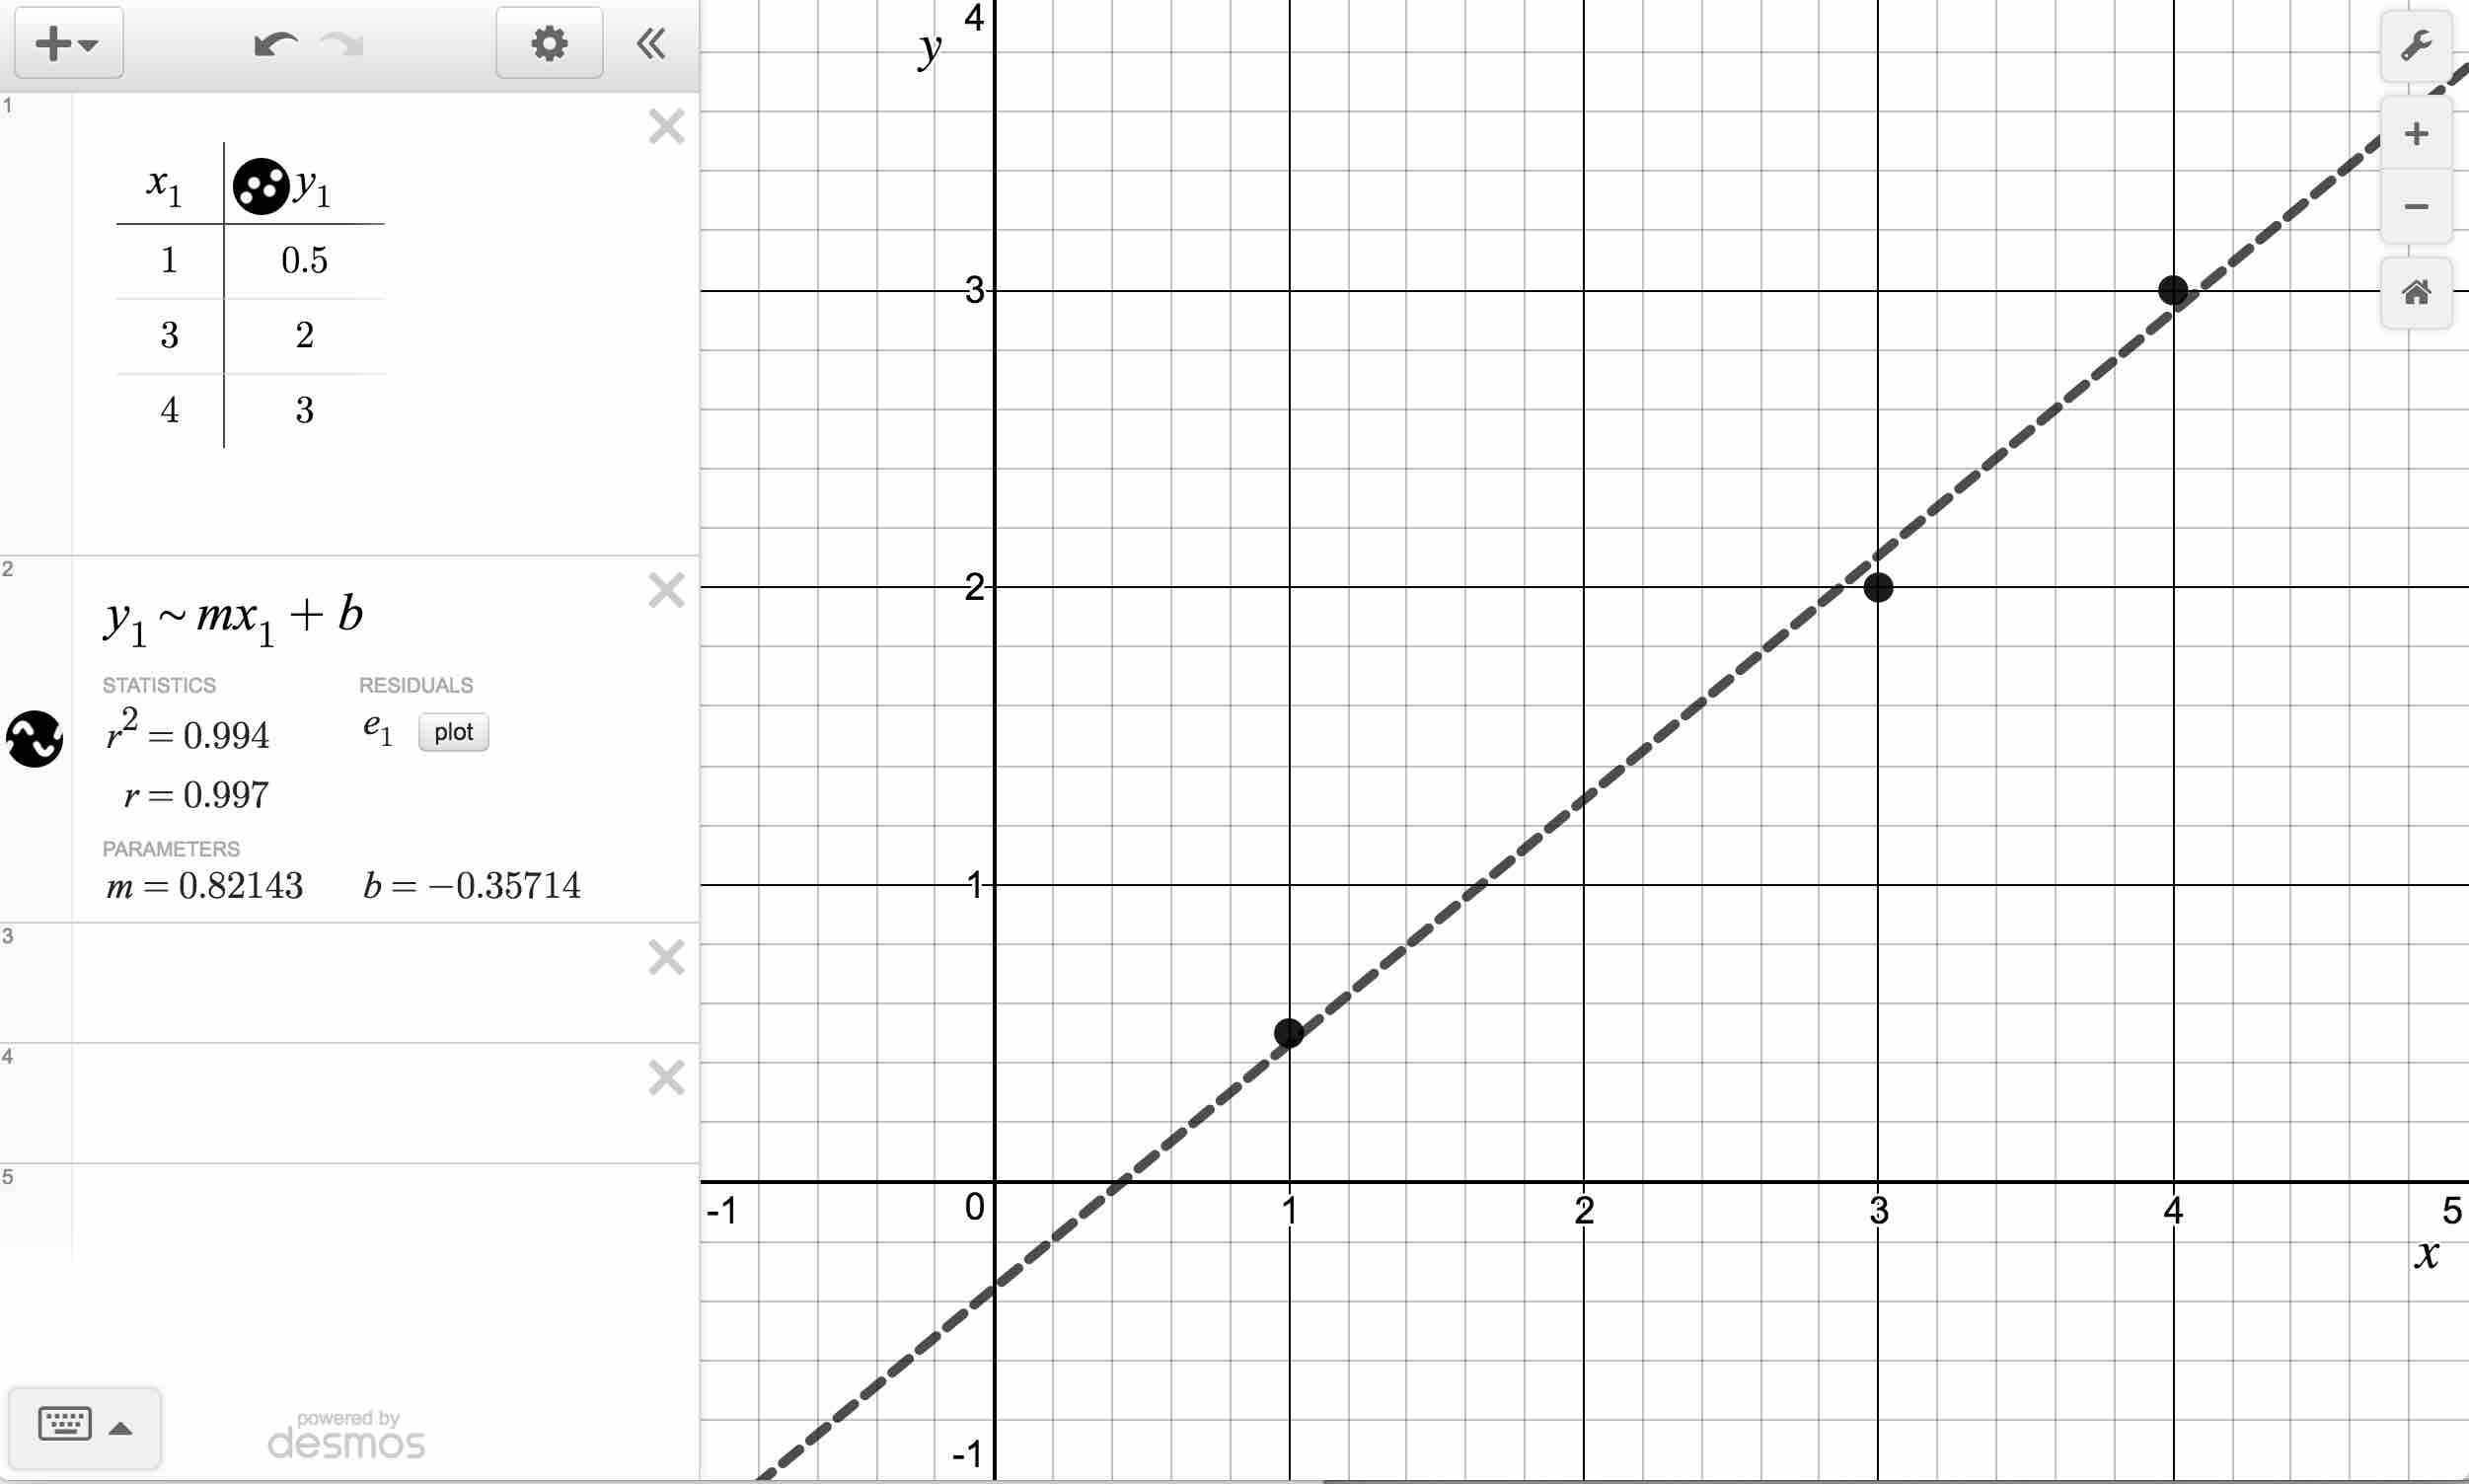
\includegraphics[width=4in]{./ConstantandLinearFunctionsGraphics/ThreePointRegression.jpg} \\
 
\end{tabular}

\medskip
\enlargethispage{.25in}

Our graphing utility produces the model\footnote{We chose to use three decimal places for the approximations in this demonstration.  How many you get to use in reality varies from one application to another.} $y=mx+b$ where the slope is $m \approx 0.821$ and the $y$-coordinate of the $y$-intercept is $b \approx -0.357$.  The value $r$ is the \index{regression ! correlation coefficient}\index{correlation coefficient}\textbf{correlation coefficient} and is a measure of how close the data is to being on the same line.  The closer $|r|$ is to $1$, the better the linear fit.\footnote{The value $r^2$ is called the \index{regression ! coefficient of determination}\index{coefficient of determination}\textbf{coefficient of determination} and is also a measure of the goodness of fit. We refer the interested reader to a course in Statistics to explore the significance of $r$ and $r^2$.} Having $r \approx 0.997$ tells us that the points have a strong, positive correlation - that is, they are very close to being on a line with a positive slope, namely $y = 0.821x - 0.357$.   Indeed, the total squared error between our data set and this line is $E \approx 0.018$. The mathematics tells us that this is the smallest we can get $E$ by modifying the parameters $m$ and $b$, even though none of the data points actually lie on the line.  

\medskip

Now that we have this new mathematical machinery, let's revisit Skippy's time and temperature data.
  
\begin{ex} \label{timetempregressionex}  $~$
  
\begin{enumerate}
  
\item Use a graphing utility to find best fit linear models for each of the data sets below. Comment on the fit and interpret the slope of each.

\begin{center}
  
\begin{multicols}{2}
  
$\begin{array}{|c||c|}  \hline

 \text{$t$: hours after 6 a.m.}  & \text{$T$: temperature $^{\circ}$F} \\ \hline
 0 & 64  \\  \hline
 2 & 67  \\  \hline
 4 &  75  \\  \hline
 6 &  80 \\  \hline
 8 & 83  \\  \hline

\end{array}$
  

	
$\begin{array}{|c||c|}  \hline

 \text{$t$: hours after 6 a.m.}  & \text{$T$: temperature $^{\circ}$F} \\ \hline

 8 & 83  \\  \hline
 10 &  83 \\  \hline
 12 & 82  \\  \hline

\end{array}$ 
  
\end{multicols}
  
\end{center}

\item  Use your models to predict the temperature at $7$ a.m. and $3$ p.m., rounded to one decimal place.
  
\end{enumerate}

\pagebreak

{\bf Solution.}
  
\begin{enumerate}
  
 \item For our first set of data, we get the line $T = F(t) = 2.55t + 63.6$.  The value $r = 0.987$ tells us that it is a fairly good fit and we see this graphically, too.\footnote{We use $F$ as the name of the function here to distinguish it from $f$ - the function determined solely by the given set of data.}   Thus we can be confident in using this model to predict the temperature during between the hours of 6 a.m. and 2 p.m. with reasonable accuracy.   

\medskip

To interpret the slope, we recognize $t$ as the independent variable (input) and $T$ as the dependent variable (output), so the slope $m = \frac{\Delta T}{\Delta t}$ is the rate of change of temperature with respect to time.   In this case,  $m = 2.55$ means that the temperature is increasing (getting warmer) at a rate of $2.55^{\circ}$F per hour.  A screenshot from Desmos is given below.

\begin{center}
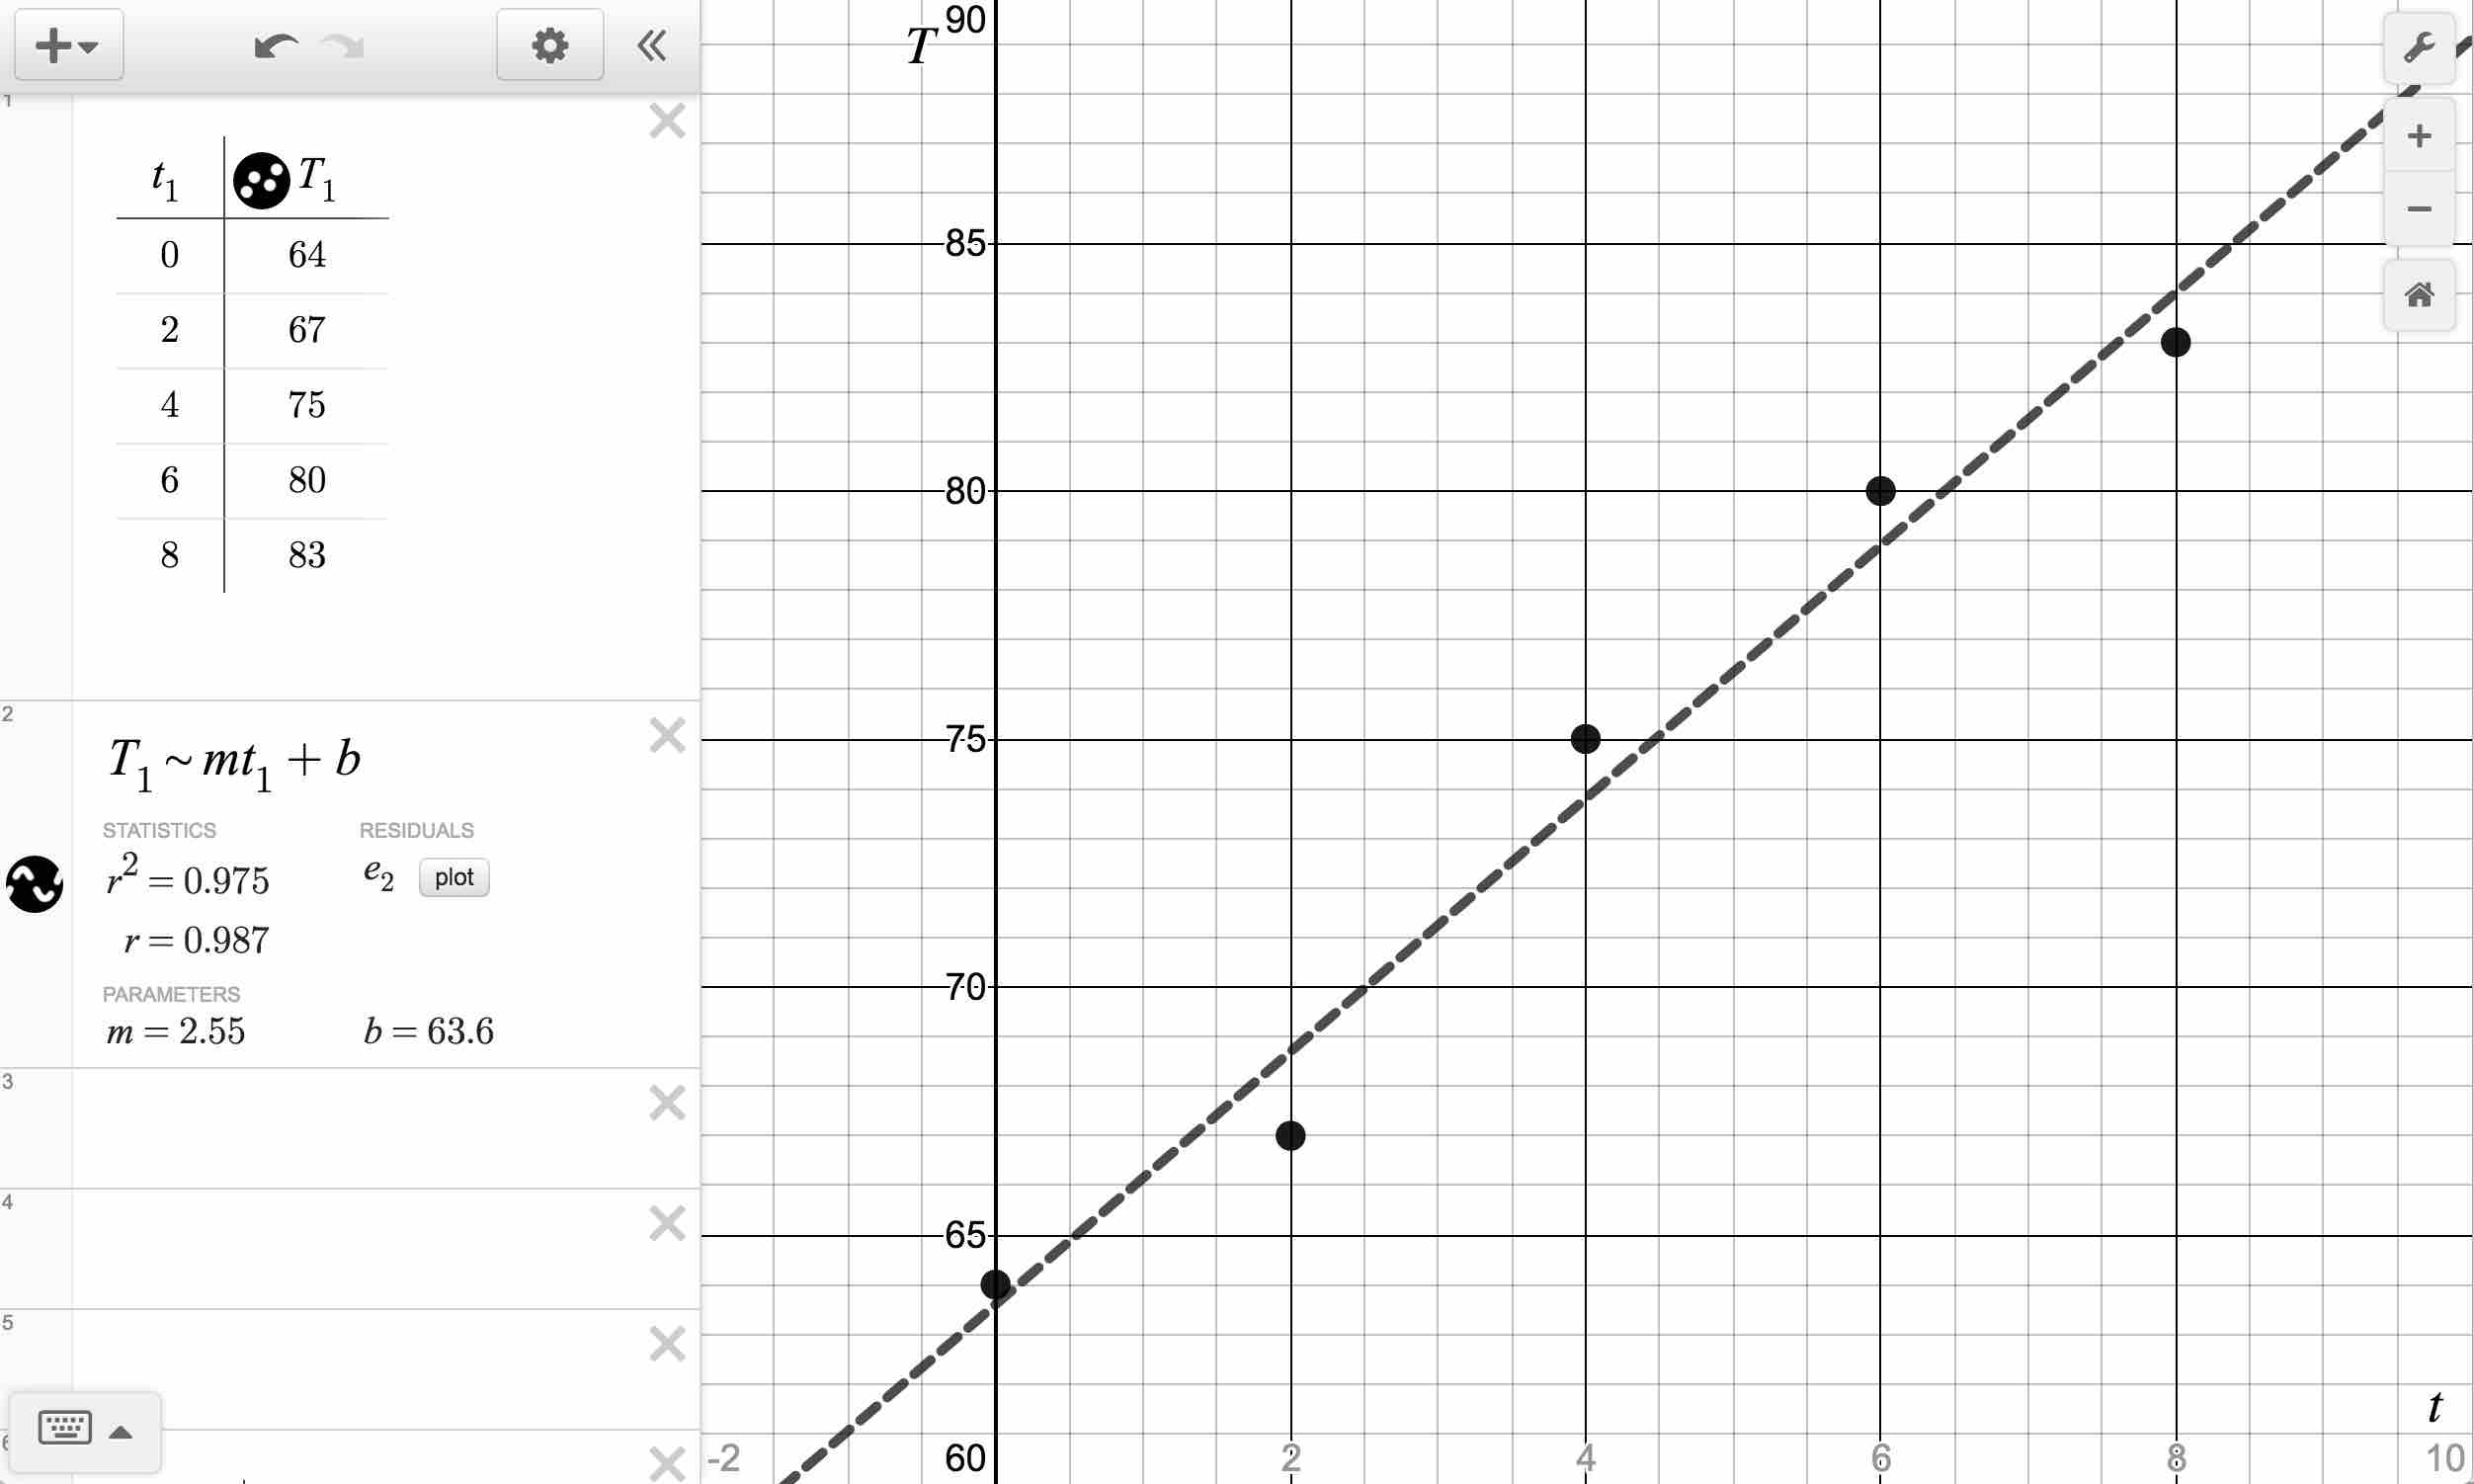
\includegraphics[width=6in]{./ConstantandLinearFunctionsGraphics/TimeTempRegression01.jpg}
\end{center}
  
For the second set of data, we get $T = G(t) = -0.25t + 85.167$ and we have $r = -0.866$.  Here, the negative sign on $r$ indicates a negative correlation which means our line has a negative slope.\footnote{We use $G$ as the function name here to distinguish it from the given function $f$ and the regression for the first data set, $F$.} While the fit looks OK, it certainly isn't as strong as with the first data set, so using this model to predict the temperature between $2$ p.m. and $6$ p.m. (let alone beyond) is a bit risky.  

\medskip

The slope in this case is $m = -0.25$ which corresponds to the temperature decreasing (getting cooler) at a rate of  $0.25^{\circ}$F per hour.  That's what a negative correlation means - an increase in input (more time passes) yields a decrease in output (cooler temperatures).  As screenshot from Desmos is given at the top of the next page.
  
\begin{center}
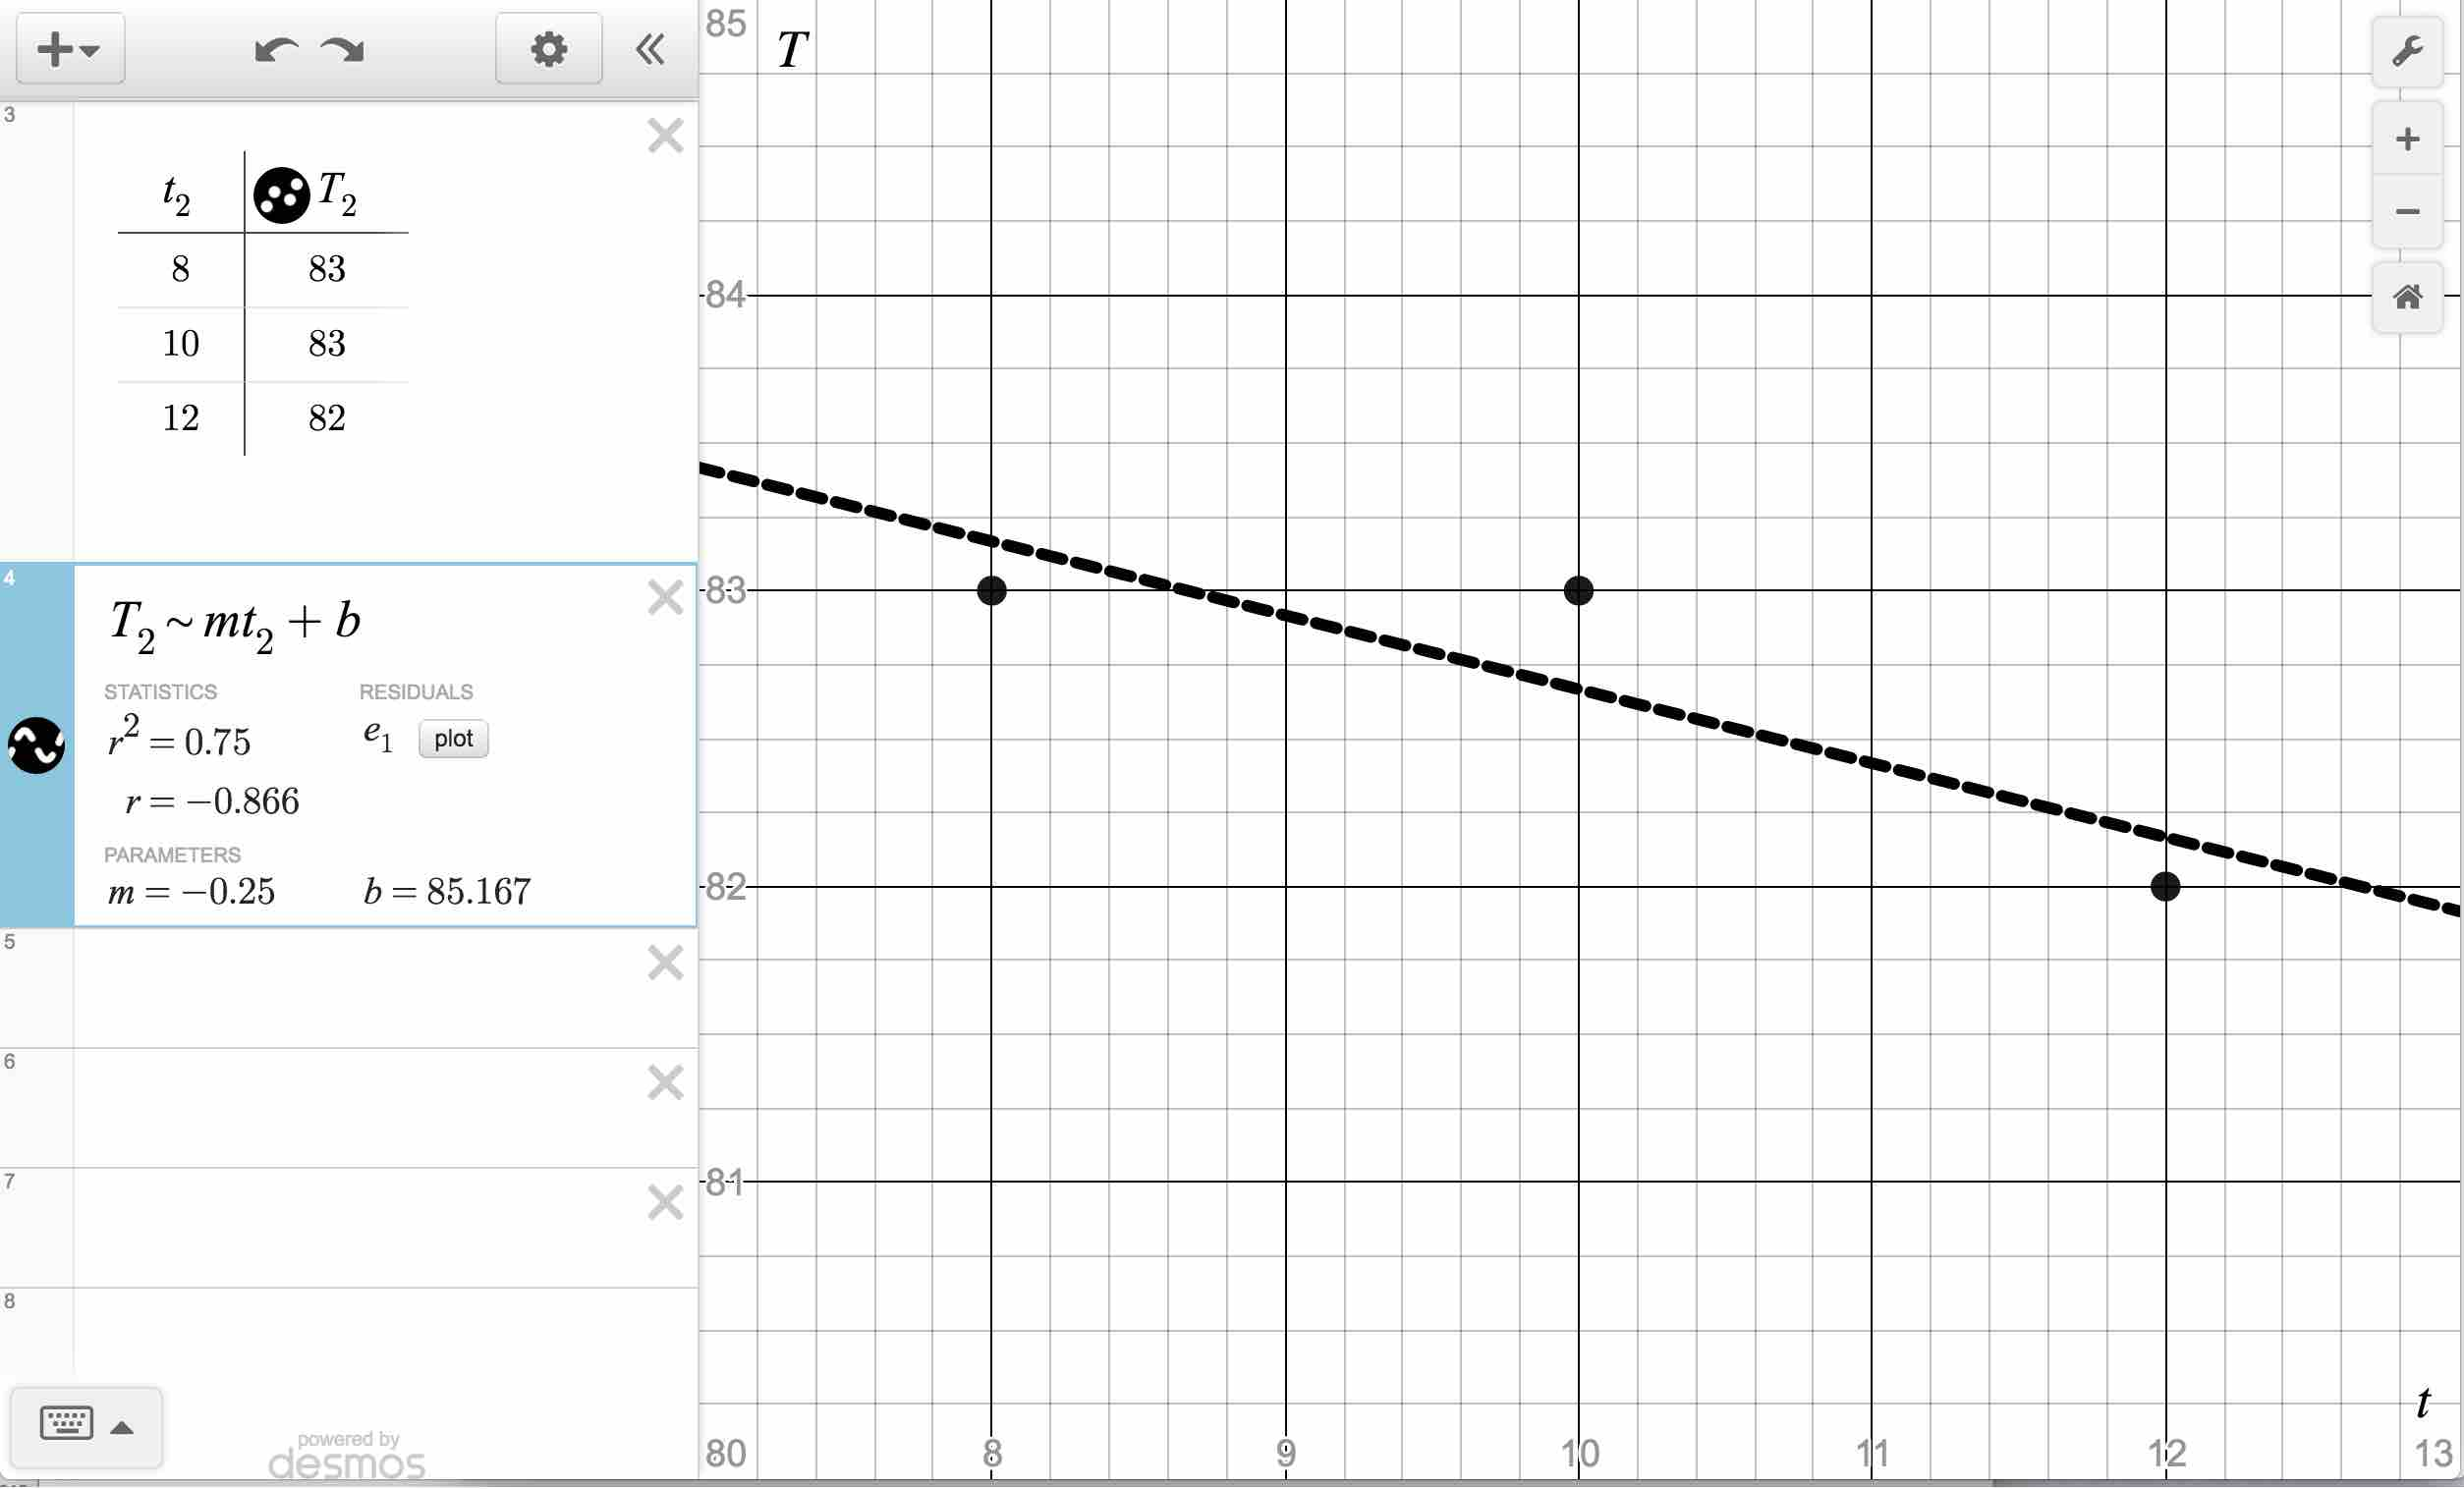
\includegraphics[width=6in]{./ConstantandLinearFunctionsGraphics/TimeTempRegression02.jpg}
\end{center}

\item  The time $7$ a.m. corresponds to $t = 1$. This falls between $t = 0$ and $t = 8$ so we use our first model.  Substituting $t = 1$ gives $T = F(1) = 2.55(1) + 63.6 \approx 66.2$.  Therefore, the model predicts the temperature to be $66.2^{\circ}$F at 7 a.m..  Likewise, $3$ p.m. corresponds to $t = 9$.  This is greater than $8$, so we use the second model: $T = G(9) =  -0.25(9) + 85.167 \approx  82.9$.  The model predicts the temperature at $3$ p.m. to be $82.9^{\circ}$F.   Based on the goodness of fit of each model, we have more confidence in the former prediction than in the latter.   \qed
  
\end{enumerate}
\end{ex}
 
Examples \ref{PortaBoyCost}, \ref{PortaBoyDemand} and \ref{timetempregressionex} (among others)  represent three different levels of mathematical modeling.  In Example  \ref{PortaBoyCost},  the mathematical model (the cost function) was provided and our task was to use the model to \textit{interpret} the mathematics in that context.    In Example  \ref{PortaBoyDemand}, we were given a minimal amount of information, namely, two data points, and then asked to \textit{construct} a model which fit those data exactly.  Lastly, in Example \ref{timetempregressionex}, we were given several data points and we used statistical methods to construct a \textit{best fit} model to the data. 

\medskip

The validity of the models rests on the validity of the underlying assumptions used to create the models.  For instance, is there any reason to assume a price-demand function would be linear?  Is it reasonable to assume that the temperature changes at a constant rate? These are questions for economists and scientists.  Mathematicians often take on a role of equal parts translator and prophet:  they codify ideas into formulas and then use them to make predictions about yet-to-be observed phenomena.  

\pagebreak

\subsection{The Average Rate of Change of a Function}
\label{AverageRateofChange}

As mentioned earlier in the section, the concepts of slope and the more general rates of change are important concepts not just in Mathematics, but also in other fields.   Many important phenomena are modeled using non-linear functions, and while the rates of change of these functions are not constant, we can sample the function at two points and compute what is known as an \textbf{average rate of change} between them to give some sense as to the function's behavior over that interval.\footnote{We are basically pretending that the function is linear on a short interval to see what we can say about its behavior.}

\medskip

\colorbox{ResultColor}{\bbm

\begin{defn} \label{arc}  Let $f$ be a function defined on the interval $[a,b]$.  The \index{average rate of change}\index{rate of change ! average}\textbf{average rate of change}  of $f$ over $[a,b]$ is defined as: \[ \dfrac{\Delta [f(x)]}{\Delta x} = \dfrac{f(b) - f(a)}{b-a} \]

Geometrically, the average rate of change is the slope of the line\footnote{This line is called a \textit{secant} line.}  containing $(a, f(a))$ and $(b, f(b))$.
\end{defn}

\ebm}

\medskip

As with Definitions \ref{absmaxmindefn}  and \ref{incdeccnstdefn}, the wording in Definition \ref{arc}, while referring to the function $f$, is really making a statement about its outputs $f(x)$.  

\medskip

If $f$ is increasing over $[a,b]$, then the average rate of change will be positive. Likewise, if $f$ is decreasing or constant, the average rate of change will be negative or $0$, respectively. (Think about this for a moment.) However, as the next example demonstrates, the converses of these statements aren't always true.\footnote{For example, the average rate of change over an interval could be positive yet the function could decrease over part of that interval and then increase on a different part.}

\begin{ex} \label{ARCRocketExample} The formula $s(t) = -5t^{\,2} + 100t$ for $0 \leq t \leq 20$ gives the height, $s(t)$, measured in feet, of a model rocket above the Moon's surface as a function of the time $t$, in seconds after lift-off.

\begin{enumerate}

\item Find $s(0)$, $s(5)$, $s(10)$, $s(15)$ and $s(20)$ and use these along with a graphing utility to graph $y = s(t)$.

\item State the range of $s$ and interpret the extrema, if any exist.

\item Find and interpret the $t$- and $y$-intercepts.  

\item Find and interpret the interval(s) over which $s$ is increasing, decreasing or constant.  

\item Find and interpret the average rate of change of $s$ over the intervals $[0,5]$, $[5,10]$, $[10, 20]$ and $[5, 15]$.


\end{enumerate}

{\bf Solution.}

\begin{enumerate}

\item  To find $s(0)$, we substitute $t=0$ into the formula for $s(t)$:  $s(0) = -5(0)^2+100(0) = 0$.  Similarly,  $s(5) = -5(5)^2+100(5) = -5(25)+500 = -125+500 = 375$.  Continuing, we obtain: $s(10) = 500$, $s(15) = 375$ and $s(20) = 0$.  Using these, we construct a table of values and with the help of a graphing utility we obtain:

\begin{center}
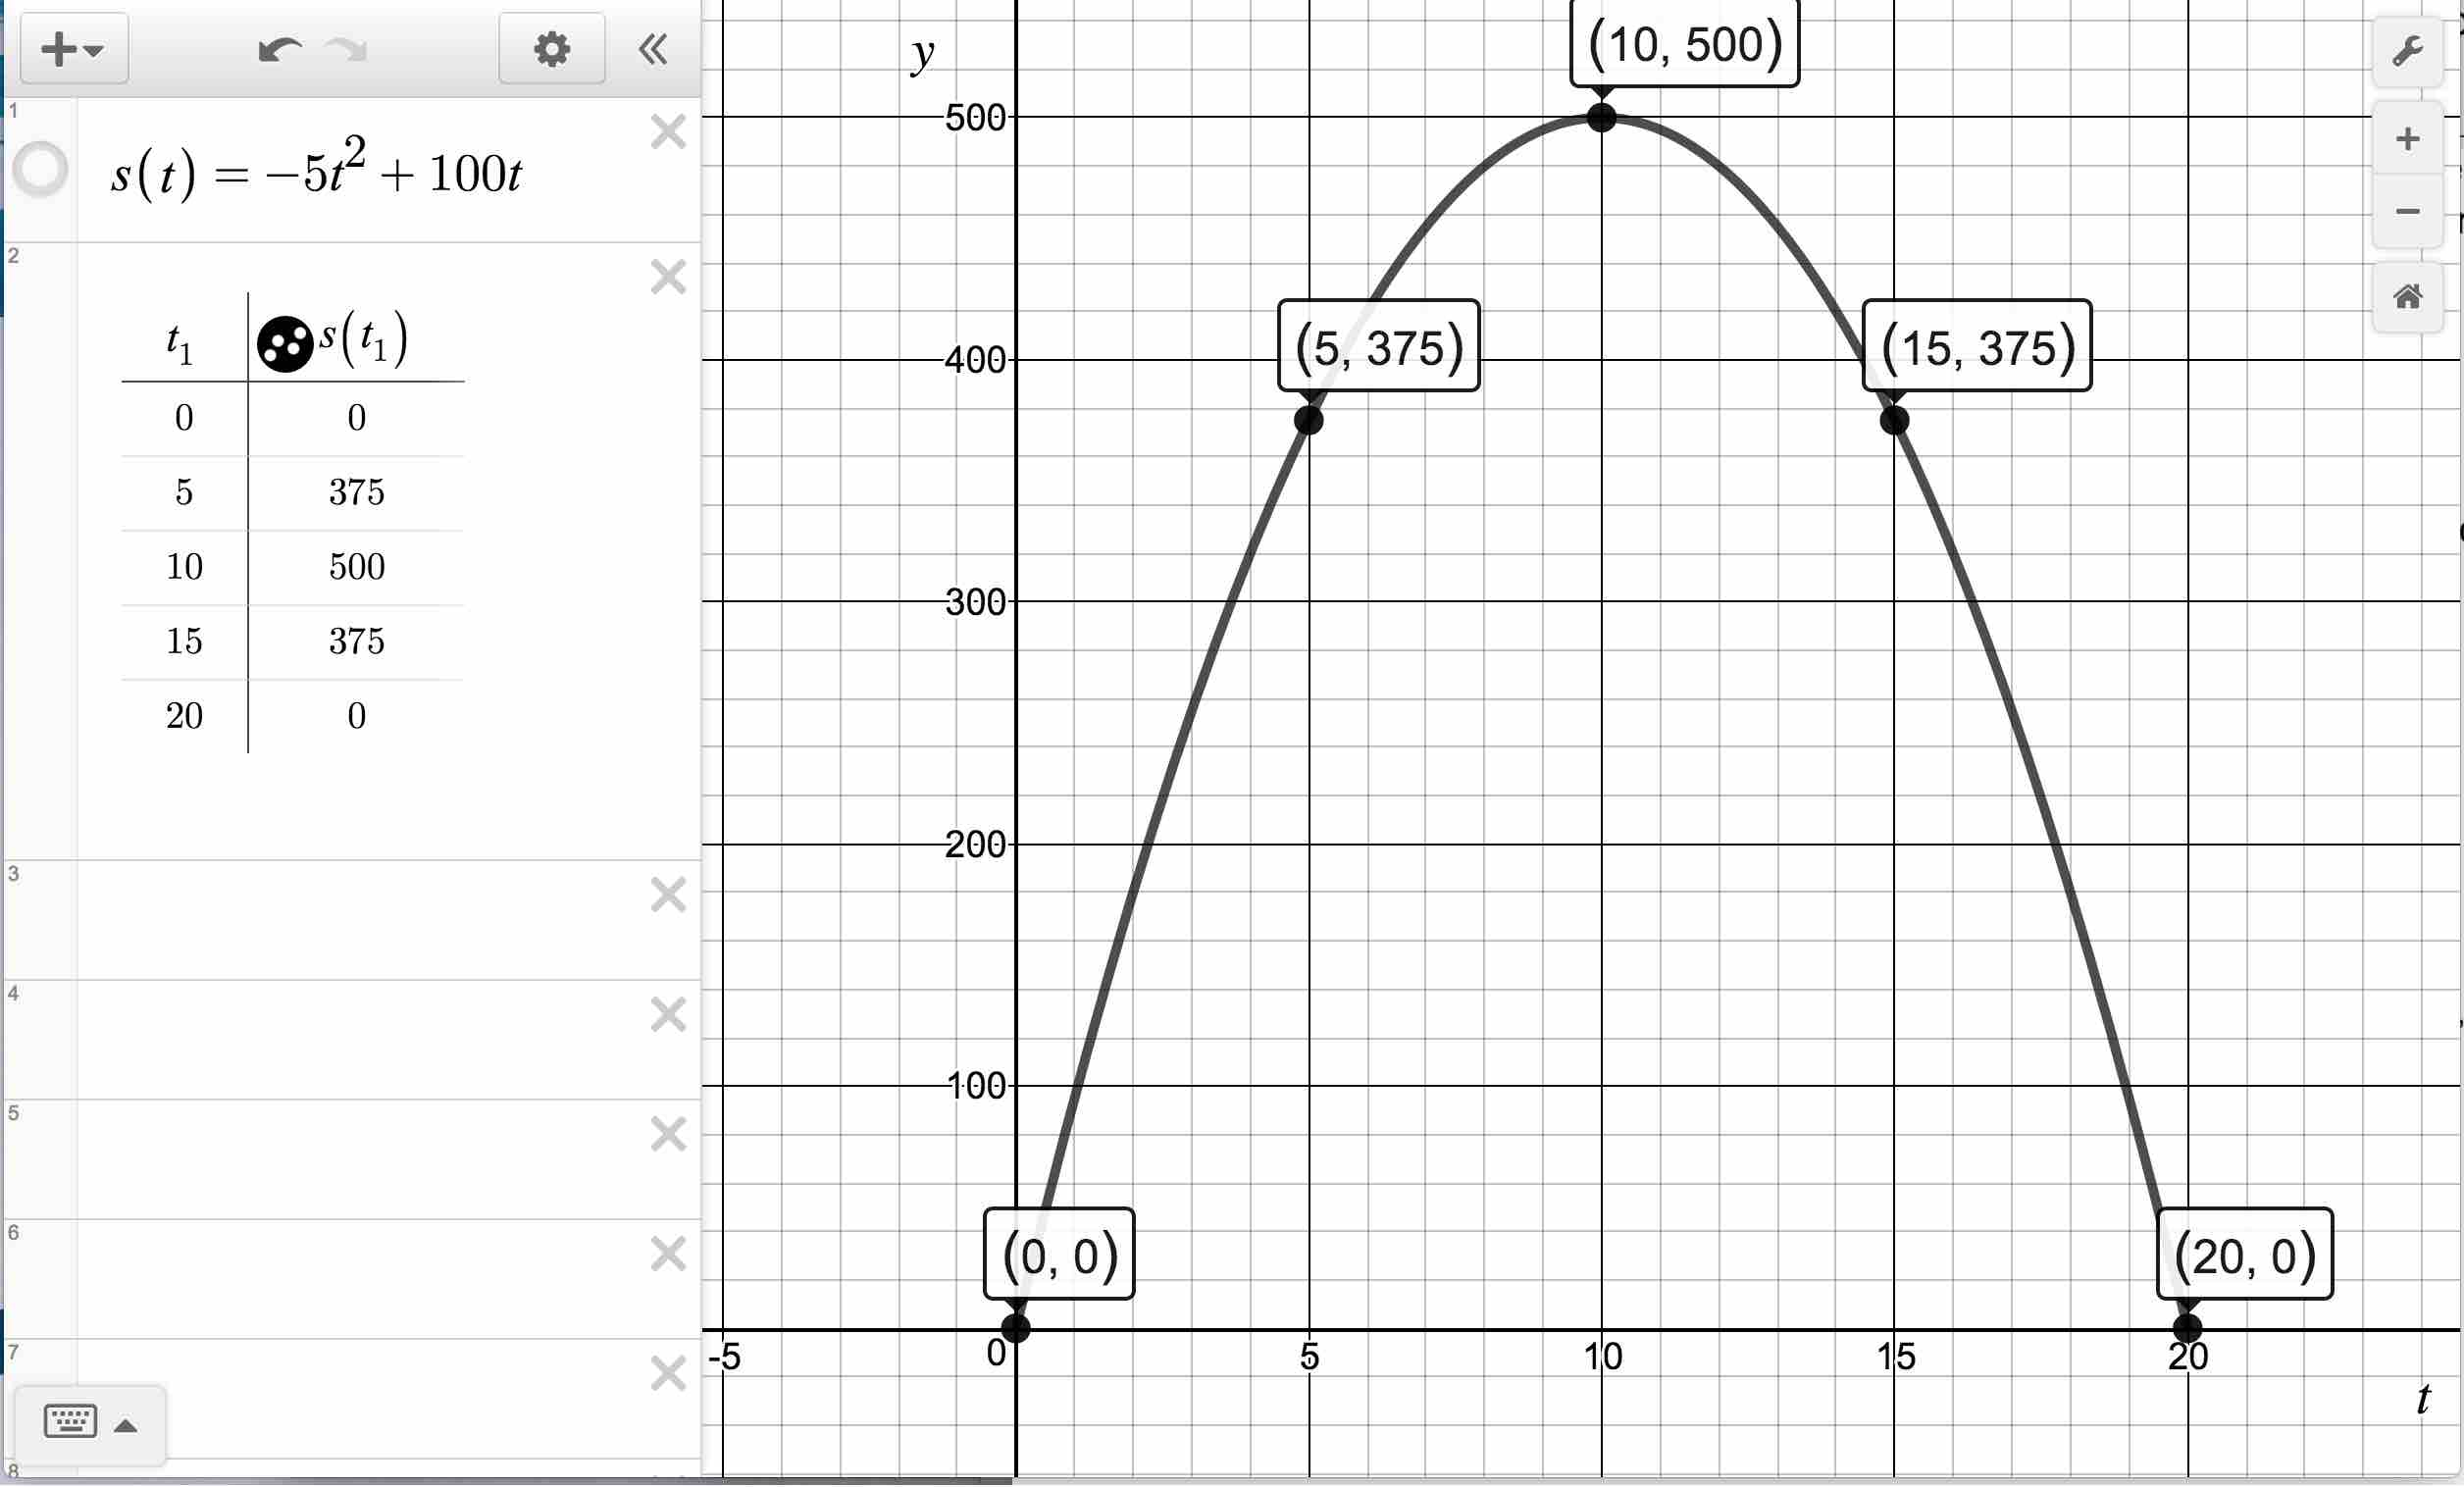
\includegraphics[width=6in]{./ConstantandLinearFunctionsGraphics/ARCRocketExample01.jpg}

\end{center}

\item  Projecting the graph to the $y$-axis, we see that the range of $s$ is $[0, 500]$ so the minimum of $s$ is $0$ and the maximum is $500$.  This means that the rocket at some point is on the surface of the Moon and reaches its highest altitude of $500$ feet above the lunar surface.

\item The first intercept we see is $(0, 0)$ which is both a $t$- and a $y$-intercept.  Given that $t$ represents the time after lift-off and $y = s(t)$ represents the height above the Moon's surface, the point $(0, 0)$ means that the model rocket was launched ($t=0$) from the Moon's surface ($s(t) = 0$).  The remaining intercept, $(20, 0)$,  is another $t$-intercept.  This means that $20$ seconds after lift-off ($t=20$), the model rocket returns to the Moon's surface ($s(t) = 0$).   Said differently, $20$ seconds is the `time of flight' of the model rocket.

\item  Referring to Definition \ref{incdeccnstdefn}, $s$ increases over the interval $[0, 10]$, since for those values of $t$, as we read from left to right, the graph of the function is rising meaning the $y$ values (hence $s(t)$ values) are getting larger. Thus the model rocket is heading upwards for the first $10$ seconds of its flight.  We find that $s$ decreases over the interval $[10, 20]$, indicating once it has reached its highest altitude of $500$ feet $10$ seconds into the flight, the rocket begins to fall back to the surface of the Moon, landing $20$ seconds after lift-off.

\item  To find the average rate of change of $s$ over the interval $[0, 5]$ we compute \[ \dfrac{\Delta[s(t)]}{\Delta t} = \dfrac{s(5) - s(0)}{5 - 0} = \dfrac{\text{$375$ feet}}{\text{$5$ seconds}} = \text{$75$ feet per second}.\] In other words, the height is \textit{increasing} at an \textit{average rate} of $75$ feet per second during the first 5 seconds of flight.  The rate here is called the\index{average velocity} \index{velocity ! average} \textbf{average velocity} of the rocket over this interval.  Velocity differs from speed in that velocity comes with a direction.  In this case, a positive velocity indicates that the rocket is traveling \textit{upwards}, since when $s$ is increasing, the model rocket is climbing higher.  

\medskip

Similarly, the average rate of change of $s$ over the interval $[5, 10]$ works out to be $25$.  This means that the average velocity over the next $5$ seconds of the flight has slowed to $25$ feet per second. The model rocket is still, on average, traveling upwards, albeit more slowly than before.  

\medskip

Over the interval $[10, 20]$, the average rate of change of $s$ works out to be $-50$.  This means that, on average, the rocket is \textit{falling} at a rate of $50$ feet per second.  The rocket has managed to fall from its highest point $500$ feet above the surface of the Moon back to the Moon's surface in $10$ seconds so this makes sense. Last, but not least, the average rate of change of $s$ over $[5, 15]$ turns out to be $0$.  This means that the model is the same height above the ground after $5$ seconds ($375$ feet) as it is after $15$ seconds.    

\medskip

Geometrically, the average rate of change of a function over an interval can be interpreted as the slope of a secant line. Below on the left is a dotted line containing $(0, 0)$ and $(5, 375)$ (which has slope $75$) along with a dotted line containing the points $(5, 375)$ and $(10, 500)$ (which has slope $25$).  Visually, the lines help demonstrate that, while $s$ is increasing over $[0, 10]$, the rate of increase is slowing down as $t$ nears $10$.  

\medskip

The graph below on the right depicts a dotted line through $(10, 500)$ and $(20,0)$ indicating a net decrease over that interval.  We also have a horizontal line ($0$ slope) containing the points $(5, 375)$ and $(15, 375)$, which shows no net change between those two points, despite the fact that the rocket rose to its maximum height then began its descent during the interval $[5, 15]$.  

\medskip

\begin{multicols}{2}


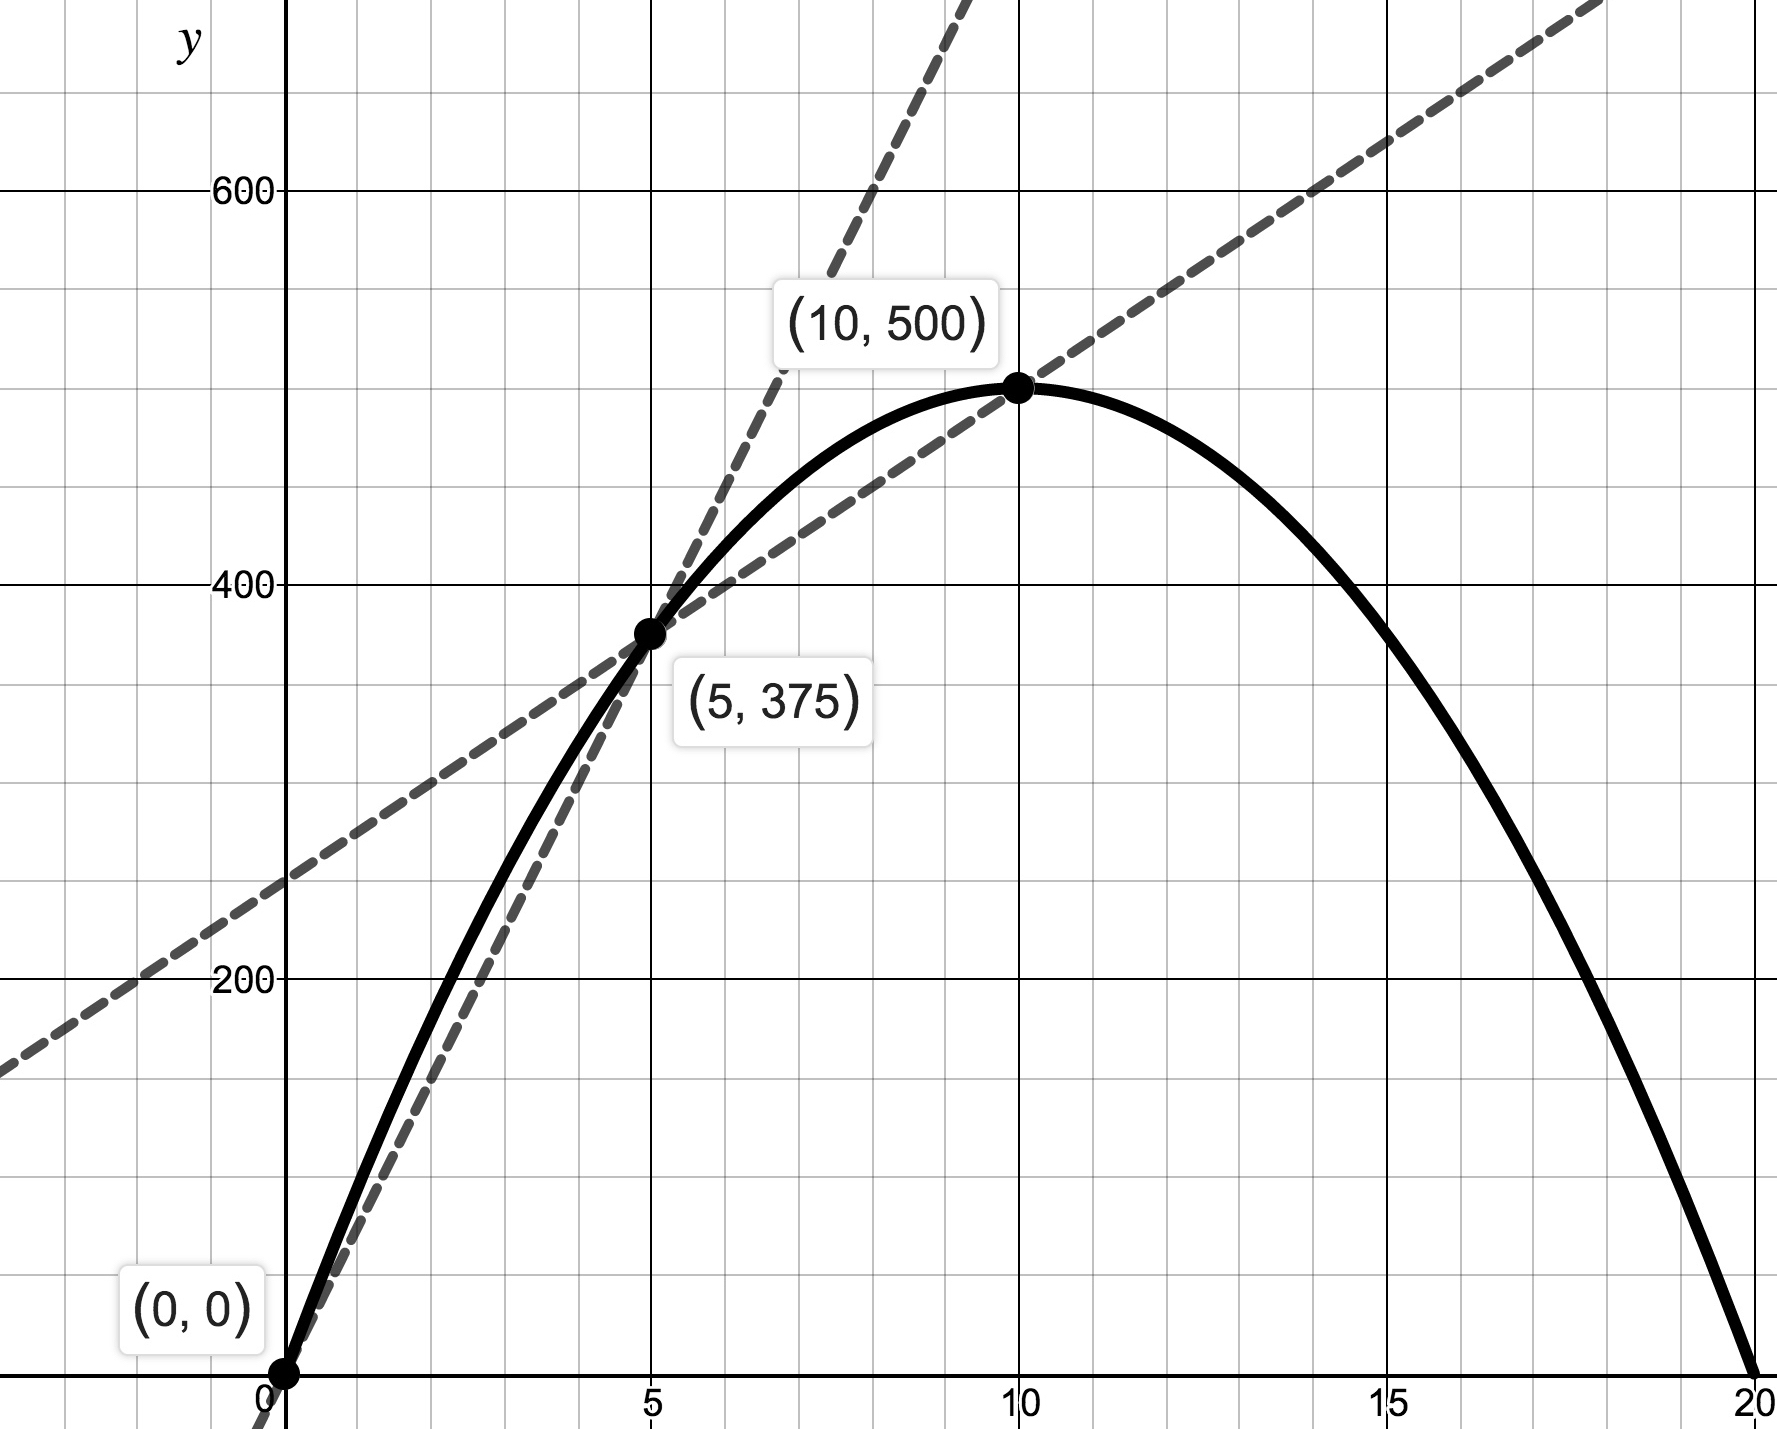
\includegraphics[width=3in]{./ConstantandLinearFunctionsGraphics/ARCRocketExample02.jpg}

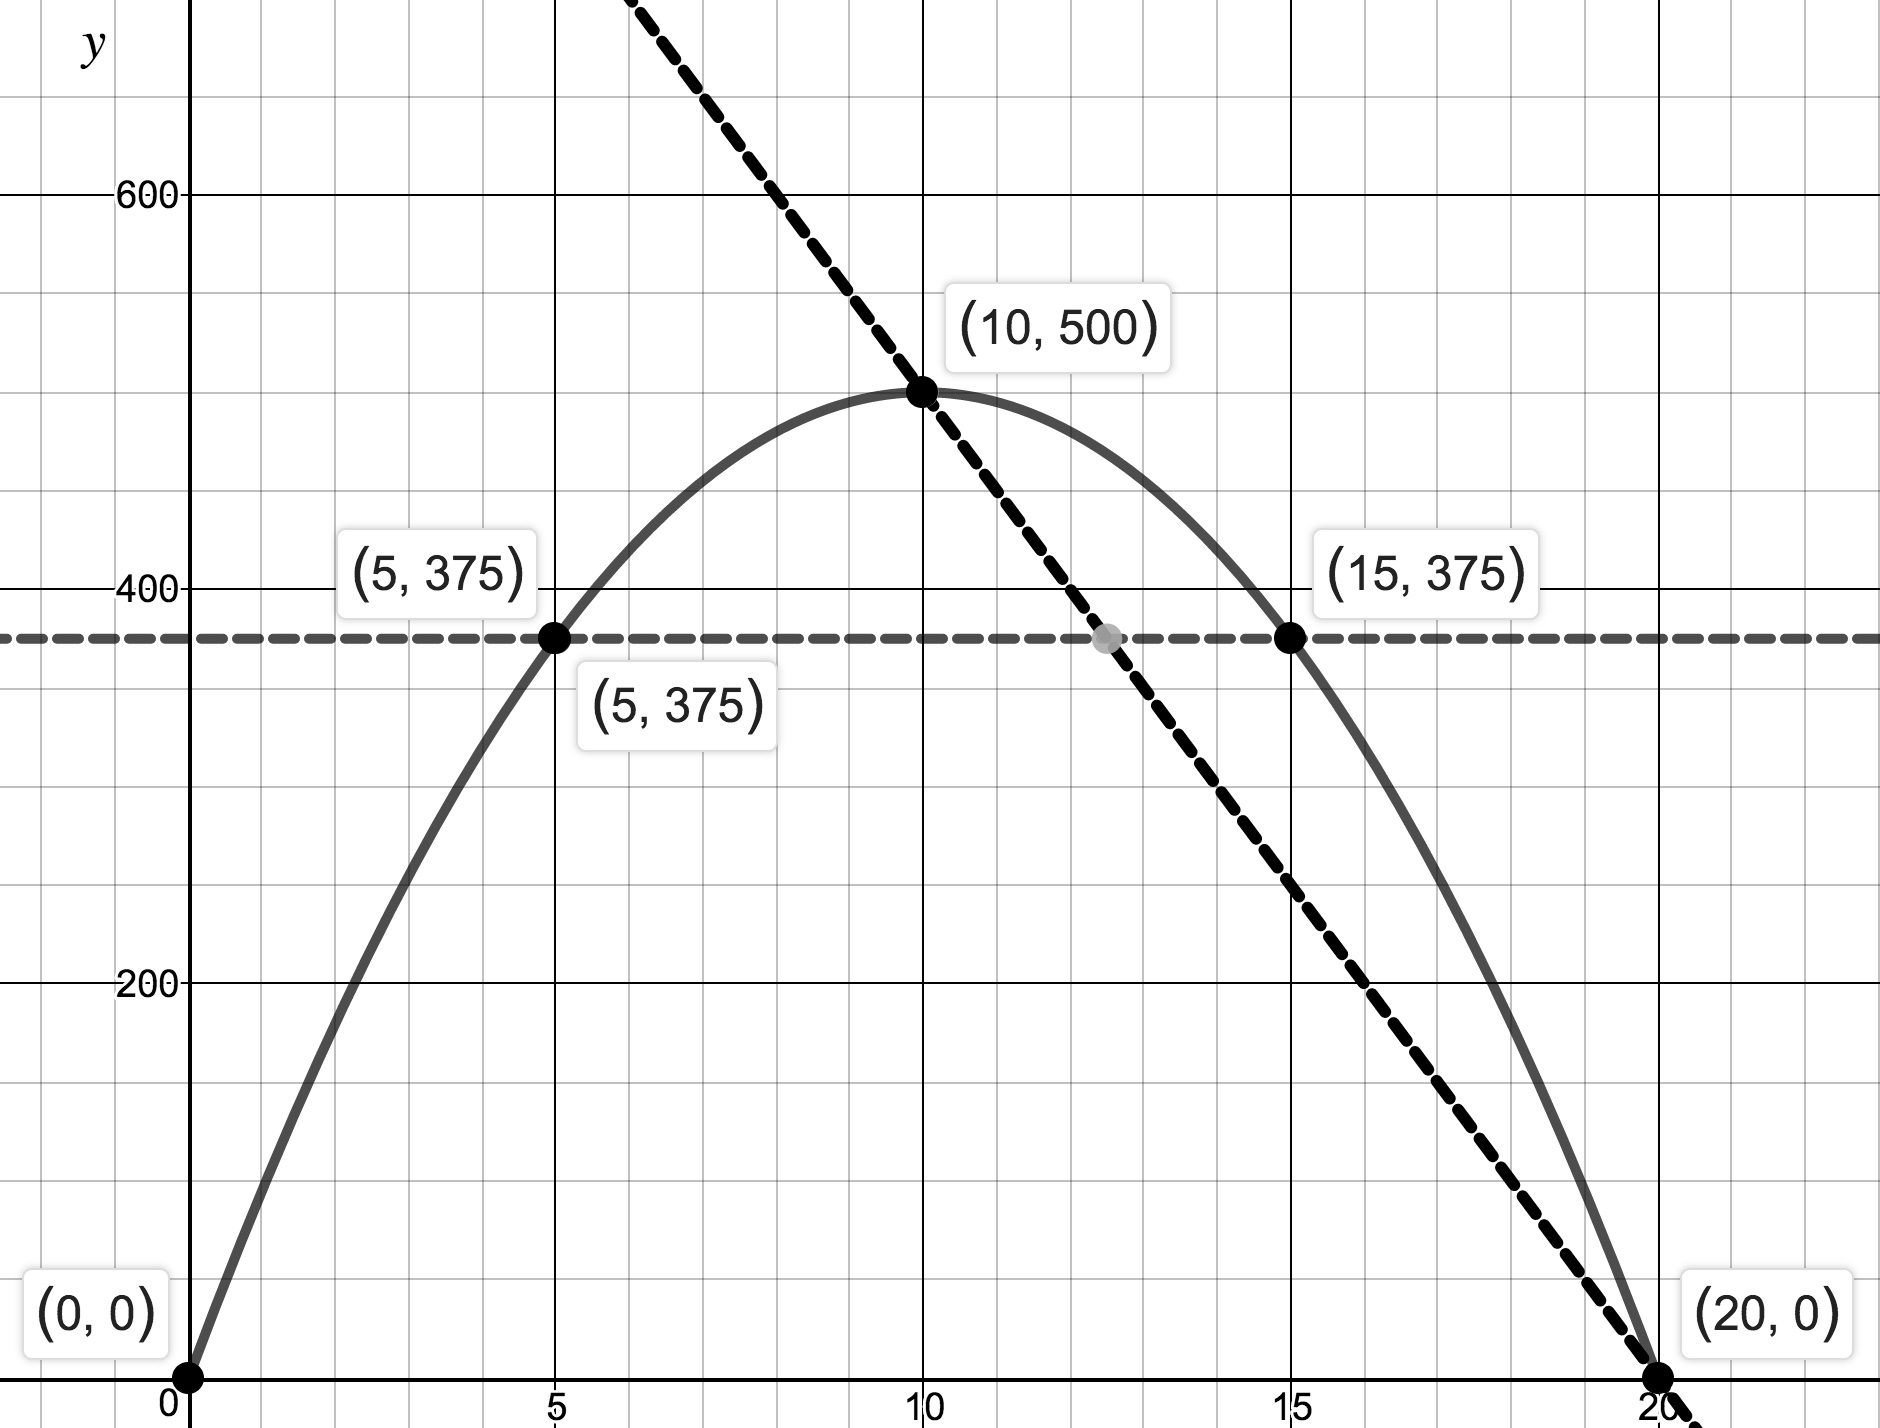
\includegraphics[width=3in]{./ConstantandLinearFunctionsGraphics/ARCRocketExample03.jpg}


\end{multicols}

\end{enumerate}

\vspace{-.2in} \qed

\end{ex}

An important lesson from the last example is that average rates of change give us a snapshot of what is happening \textit{at the endpoints} of an interval, but not necessarily what happens \textit{over the course} of the interval.  Calculus gives us tools to compute slopes \textit{at} points which correspond to  \textit{instantaneous} rates of changes.  While we don't quite have the machinery to properly express these ideas, we can hint at them in the Exercises. Speaking of exercises \ldots 

\newpage

\subsection{Exercises}

In Exercises \ref{graphlinearfunctionfirsta} - \ref{graphlinearfunctionlasta}, graph the function.  Find the slope and  axis intercepts, if any.

\begin{multicols}{2}
\begin{enumerate}


\item $f(x) = 2x - 1$ \label{graphlinearfunctionfirsta}
\item $g(t) = 3 - t$

\setcounter{HW}{\value{enumi}}
\end{enumerate}
\end{multicols}

\begin{multicols}{2}
\begin{enumerate}
\setcounter{enumi}{\value{HW}}

\item $F(w) = 3$
\item $G(s) = 0$

\setcounter{HW}{\value{enumi}}
\end{enumerate}
\end{multicols}

\begin{multicols}{2}
\begin{enumerate}
\setcounter{enumi}{\value{HW}}

\item $h(t) = \frac{2}{3} t + \frac{1}{3}$ \vphantom{$\dfrac{1-x}{2}$}
\item $j(w) = \dfrac{1-w}{2}$  \label{graphlinearfunctionlasta}

\setcounter{HW}{\value{enumi}}
\end{enumerate}
\end{multicols}

In Exercises \ref{graphpwiseexerfirst} - \ref{graphpwiseexerlast}, graph the function.  Find the domain, range, and axis intercepts, if any.

\enlargethispage{0.25in}

\begin{multicols}{2}
\begin{enumerate}
\setcounter{enumi}{\value{HW}}

\item ${\displaystyle f(x) = \left\{ \begin{array}{rcl} 4-x & \mbox{ if } &  x \leq 3 \\
                                                            2 & \mbox{ if } & x > 3
                                     \end{array} \right. }$   \label{graphpwiseexerfirst}

\item ${\displaystyle g(x) = \left\{ \begin{array}{rcl} 2-x & \mbox{ if } &  x < 2 \\
                                                            x-2 & \mbox{ if } & x \geq  2
                                     \end{array} \right. }$


\setcounter{HW}{\value{enumi}}
\end{enumerate}
\end{multicols}


\begin{multicols}{2}
\begin{enumerate}
\setcounter{enumi}{\value{HW}}

\item ${\displaystyle F(t) = \left\{ \begin{array}{rcl} -2t - 4 & \mbox{ if } &  t < 0 \\
                                                             3t & \mbox{ if } & t \geq 0
                                     \end{array} \right. }$


\item ${\displaystyle G(t) = \left\{ \begin{array}{rcl}  -3 & \mbox{ if } & t < 0 \\
                                                        2t-3 & \mbox{ if } & 0 < t < 3 \\
                                                            3 & \mbox{ if } & t > 3
                                     \end{array} \right. }$  \label{graphpwiseexerlast}



 \label{graphlineexerlast}

\setcounter{HW}{\value{enumi}}
\end{enumerate}
\end{multicols}

\begin{enumerate}
\setcounter{enumi}{\value{HW}}

\item  \label{unitstepexercise} The \index{unit step function}\textbf{unit step function} is defined as $U(t) = \begin{cases}
    0 &  \text{if $t<0$, } \\
    1  & \text{if $t \geq 0$.} \\
   \end{cases}$

\begin{enumerate}

\item  Graph $y = U(t)$.

\item  State the domain and range of $U$.

\item  List the interval(s) over which $U$ is increasing, decreasing, and/or constant.

\item  Write $U(t-2)$ as a piecewise defined function and graph.

\end{enumerate}


\setcounter{HW}{\value{enumi}}
\end{enumerate}


In Exercises \ref{findformulalinearfirstex} - \ref{findformulalinearlastex}, find a formula for the function.

\begin{multicols}{2}

\begin{enumerate}

\setcounter{enumi}{\value{HW}}

\item $~$   \label{findformulalinearfirstex}

\begin{mfpic}[15]{-5}{5}{-5}{5}
\axes
\tlabel[cc](5,-0.5){\scriptsize $x$}
\tlabel[cc](0.5,5){\scriptsize $y$}
\tlabel[cc](1, -2.75){\scriptsize $(0,-3)$}
\xmarks{-4,-3,-2,-1,1,2,3,4}
\ymarks{-4,-3,-2, -1, 1,2,3,4}
\tlpointsep{4pt}
\scriptsize
\axislabels {x}{ {$-4 \hspace{7pt}$} -4,{$-3 \hspace{7pt}$} -3, {$-2 \hspace{7pt}$} -2, {$-1 \hspace{7pt}$} -1, {$1$} 1, {$2$} 2, {$3$} 3, {$4$} 4}
\axislabels {y}{{$-4$} -4,{$-2$} -2, {$-1$} -1,{$1$} 1, {$2$} 2, {$3$} 3, {$4$} 4}
\penwd{1.25pt}
\arrow \reverse \arrow \polyline{( -5,-3), (5,-3)}
\point[4pt]{(0,-3)}
\tcaption{ \scriptsize$y = f(x)$}
\normalsize
\end{mfpic}



\item $~$


\begin{mfpic}[15]{-5}{5}{-5}{5}
\axes
\tlabel[cc](5,-0.5){\scriptsize $t$}
\tlabel[cc](0.5,5){\scriptsize $s$}
\tlabel[cc](1, 1.5){\scriptsize $(1,2)$}
\tlabel[cc](1, -3.5){\scriptsize $(1,-3)$}
\tlabel[cc](3, -2.5){\scriptsize $(3,-3)$}
\tlabel[cc](3, 3.5){\scriptsize $(3,4)$}
\xmarks{-4,-3,-2,-1,1,2,3,4}
\ymarks{-4,-3,-2, -1, 1,2,3,4}
\tlpointsep{4pt}
\scriptsize
\axislabels {x}{ {$-4 \hspace{7pt}$} -4,{$-3 \hspace{7pt}$} -3, {$-2 \hspace{7pt}$} -2, {$-1 \hspace{7pt}$} -1, {$1$} 1, {$2$} 2, {$3$} 3, {$4$} 4}
\axislabels {y}{{$-4$} -4,{$-3$} -3,{$-2$} -2, {$-1$} -1,{$1$} 1,  {$3$} 3, {$4$} 4}
\penwd{1.25pt}
\arrow \polyline{(1,2), (-5,2)}
 \polyline{(1,-3), (3,-3)}
 \arrow \polyline{(3,4), (5,4)}
\tcaption{ \scriptsize$s = F(t)$}
\point[4pt]{(1,2), (3,-3)}
\pointfillfalse
\point[4pt]{(1,-3), (3,4)}
\normalsize
\end{mfpic}


\setcounter{HW}{\value{enumi}}

\end{enumerate}

\end{multicols}

\begin{multicols}{2}

\begin{enumerate}

\setcounter{enumi}{\value{HW}}

\item $~$


\begin{mfpic}[15]{-5}{5}{-5}{5}
\axes
\tlabel[cc](5,-0.5){\scriptsize $x$}
\tlabel[cc](0.5,5){\scriptsize $y$}
\tlabel[cc](-1, 0.75){\scriptsize $(0,1)$}
\tlabel[cc](1.25, -0.75){\scriptsize $\left( \frac{5}{3}, 0 \right)$}
\xmarks{-4,-3,-2,-1,1,2,3,4}
\ymarks{-4,-3,-2, -1, 1,2,3,4}
\tlpointsep{4pt}
\scriptsize
\axislabels {x}{ {$-4 \hspace{7pt}$} -4,{$-3 \hspace{7pt}$} -3, {$-2 \hspace{7pt}$} -2, {$-1 \hspace{7pt}$} -1, {$3$} 3, {$4$} 4}
\axislabels {y}{{$-4$} -4,{$-3$} -3,{$-2$} -2, {$-1$} -1, {$2$} 2, {$3$} 3, {$4$} 4}
\penwd{1.25pt}
\arrow \reverse \arrow \polyline{( -5,4), (5,-2)}
\point[4pt]{(0,1), (1.66,0)}
\tcaption{ \scriptsize$y = L(x)$}
\normalsize
\end{mfpic}



\item $~$  \label{findformulalinearlastex}


\begin{mfpic}[15]{-5}{5}{-5}{5}
\axes
\tlabel[cc](5,-0.5){\scriptsize $v$}
\tlabel[cc](0.5,5){\scriptsize $w$}
\tlabel[cc](-3.25, -4.5){\scriptsize $(-3,-4)$}
\tlabel[cc](3, 2.5){\scriptsize $(3,2)$}
\tlabel[cc](-1.5, 2.5){\scriptsize $(-1,2)$}
\xmarks{-4,-3,-2,-1,1,2,3,4}
\ymarks{-4,-3,-2, -1, 1,2,3,4}
\tlpointsep{4pt}
\scriptsize
\axislabels {x}{ {$-4 \hspace{7pt}$} -4,{$-3 \hspace{7pt}$} -3, {$-2 \hspace{7pt}$} -2, {$-1 \hspace{7pt}$} -1, {$1$} 1,{$2$} 2, {$3$} 3, {$4$} 4}
\axislabels {y}{{$-4$} -4,{$-3$} -3,{$-2$} -2, {$-1$} -1, {$1$} 1, {$3$} 3, {$4$} 4}
\penwd{1.25pt}
\polyline{( -3,-4), (-1, 2), (3,2)}
\point[4pt]{(-3,-4),  (3,2)}
\pointfillfalse
\point[4pt]{(-1,2)}
\tcaption{ \scriptsize$w = g(v)$}
\normalsize
\end{mfpic}

\setcounter{HW}{\value{enumi}}

\end{enumerate}

\end{multicols}



\begin{enumerate}

\setcounter{enumi}{\value{HW}}



\item \label{piecewiseordering} For $n$ copies of the book \textit{Me and my Sasquatch}, a print on-demand company charges $C(n)$ dollars, where $C(n)$ is determined by the formula \[{\displaystyle C(n) = \left\{ \begin{array}{rcl}  15n & \mbox{ if } & 1 \leq n \leq 25  \\
                                                            13.50n  & \mbox{ if } & 25 < n \leq 50 \\
                                                            12n & \mbox{ if } & n > 50 \\
                                     \end{array} \right. }\]


\begin{enumerate}

\item  Find and interpret $C(20)$.

\item  \label{50vs51} How much does it cost to order 50 copies of the book?  What about 51 copies?

\item  Your answer to \ref{50vs51} should get you thinking. Suppose a bookstore estimates it will sell 50 copies of the book.  How many books can, in fact, be ordered for the same price as those 50 copies? (Round your answer to a  whole number of books.)

\end{enumerate}

\item \label{piecewiseshipping} An on-line comic book retailer charges shipping costs according to the following formula \[{\displaystyle S(n) = \left\{ \begin{array}{rcl}  1.5 n + 2.5 & \mbox{ if } & 1 \leq n \leq 14  \\
                                                            0  & \mbox{ if } & n \geq 15
                                     \end{array} \right. }\]

where $n$ is the number of  comic books purchased and $S(n)$ is the shipping cost in dollars.

\begin{enumerate}

\item  What is the cost to ship 10 comic books?

\item  What is the significance of the formula $S(n) = 0$ for $n \geq 15$?

\end{enumerate}

\newpage

\item  \label{piecewisemobile} The cost in dollars $C(m)$  to talk $m$ minutes a month on a mobile phone plan is modeled by   \[{\displaystyle C(m) = \left\{ \begin{array}{rcl} 25 & \mbox{ if } & 0 \leq m \leq 1000 \\
                                                            25+0.1(m-1000) & \mbox{ if } & m > 1000
                                     \end{array} \right. }\]

\begin{enumerate}

\item  How much does it cost to talk $750$ minutes per month with this plan?

\item  How much does it cost to talk $20$ hours a month with this plan?

\item  Explain the terms of the plan verbally.
\end{enumerate}


\setcounter{HW}{\value{enumi}}
\end{enumerate}


\begin{enumerate}

\setcounter{enumi}{\value{HW}}


\item  Jeff can walk comfortably at $3$ miles per hour.  Find an expression for a linear function $d(t)$ that represents the total distance Jeff can walk in $t$ hours, assuming he doesn't take any breaks.

\item  Carl can stuff $6$ envelopes per \textit{minute}.  Find an expression for a linear function $E(t)$ that represents the total number of envelopes Carl can stuff after $t$ \textit{hours}, assuming he doesn't take any breaks.

\item  A landscaping company charges $\$45$ per cubic yard of mulch plus a delivery charge of $\$20$.  Find an expression for a  linear function $C(x)$ which computes the total cost in dollars  to deliver $x$ cubic yards of mulch.

\item  A plumber charges $\$50$ for a service call plus $\$80$ per hour.  If she spends no longer than 8 hours a day at any one site, find an expression for a  linear function $C(t)$ that computes her total daily charges in dollars as a function of the amount of time spent in hours, $t$  at any one given location.

\item A salesperson is paid \$200 per week plus 5\% commission on her weekly sales of $x$ dollars.  Find an expression for a  linear function $W(x)$ which computes her total weekly pay in dollars as a function of $x$.  What must her weekly sales be in order for her to earn \$475.00 for the week?


\item  An on-demand publisher charges $\$22.50$ to print a 600 page book and $\$15.50$ to print a 400 page book.  Find an expression for a linear function which models the cost of a book in dollars $C(p)$ as a function of the number of pages $p$.  Find and interpret both the slope of the linear function  and $C(0)$.

\item The Topology Taxi Company charges $\$2.50$ for the first fifth of a mile and $\$0.45$ for each additional fifth of a mile.  Find an expression for a  linear function which models the taxi fare $F(m)$ as a function of the number of miles driven, $m$.  Find and interpret both the slope of the linear function  and $F(0)$.

\item Water freezes at $0^{\circ}$ Celsius and $32^{\circ}$ Fahrenheit and it boils at $100^{\circ}$C and $212^{\circ}$F.
\label{celsiustofahr}

\begin{enumerate}

\item Find an expression for a  linear function $F(T)$ that computes temperature in the Fahrenheit scale as a function of  the temperature $T$ given in degrees Celsius.  Use this function to convert $20^{\circ}$C into Fahrenheit.

\item Find an expression for a  linear function $C(T)$ that computes temperature in the Celsius scale as a function of  the temperature $T$ given in degrees Fahrenheit.  Use this function to convert $110^{\circ}$F into Celsius.

\item Is there a temperature $T$ such that $F(T) = C(T)$?

\end{enumerate}

\enlargethispage{0.5in}

\item Legend has it that a bull Sasquatch in rut will howl approximately 9 times per hour when it is $40^{\circ}F$ outside and only 5 times per hour if it's $70^{\circ}F$.  Assuming that the number of howls per hour, $N$, can be represented by a linear function of temperature Fahrenheit, find the number of howls per hour he'll make when it's only $20^{\circ}F$ outside. What troubles do you encounter when trying to determine a reasonable applied domain?

\item \label{exerredoportaboy} Economic forces have changed the cost function for PortaBoys to $C(x) = 105x + 175$.  Rework Example \ref{PortaBoyCost} with this new cost function.

\item In response to the economic forces in Exercise \ref{exerredoportaboy} above, the local retailer sets the selling price of a PortaBoy at \$250.  Remarkably, 30 units were sold each week.  When the systems went on sale for \$220, 40 units per week were sold.  Rework Example \ref{PortaBoyDemand}  with this new data.

\item A local pizza store offers medium two-topping pizzas delivered for $\$6.00$ per pizza plus a $\$1.50$ delivery charge per order.  On weekends, the store runs a `game day' special:  if six or more medium two-topping pizzas are ordered, they are $\$5.50$ each with no delivery charge.  Write a piecewise-defined linear function which calculates the cost in dollars $C(p)$ of  $p$ medium two-topping pizzas delivered during a weekend.

\item  A restaurant offers a buffet which costs $\$15$ per person.  For parties of $10$ or more people, a group discount applies, and the cost is $\$12.50$ per person.   Write a piecewise-defined linear function which calculates the total bill $T(n)$ of a party of $n$ people who all choose the buffet.

\item  A mobile plan charges a base monthly rate of $\$10$ for the first $500$ minutes of air time plus a charge of $15$\textcent \, for each additional minute.  Write a piecewise-defined linear function which calculates the monthly cost in dollars  $C(m)$  for using $m$ minutes of air time.

\textbf{HINT:}  You may wish to refer to number \ref{piecewisemobile} for inspiration.


\item  The local pet shop charges $12$\textcent \, per cricket up to 100 crickets, and $10$\textcent \, per cricket thereafter.  Write a piecewise-defined linear function which calculates the price in dollars $P(c)$ of purchasing $c$ crickets.

\item  The cross-section of a swimming pool is below.  Write a piecewise-defined linear function which describes the depth of the pool, $D$ (in feet) as a function of:

\begin{enumerate}

\item  the distance (in feet) from the edge of the shallow end of the pool, $d$.

\item  the distance (in feet) from the edge of the deep end of the pool, $s$.

\item  Graph each of the functions in (a) and (b).  Discuss with your classmates how to transform one into the other and how they relate to the diagram of the pool.

\end{enumerate}

\begin{center}

\begin{mfpic}[25]{-1}{13}{-1}{4}
\point[2pt]{(0,4), (12,4)}
\arrow \polyline{(0,4), (4,4)}
\arrow \polyline{(12,4), (8,4)}
\arrow \reverse \arrow \polyline{(-0.25,0), (-0.25,3)}
\arrow \reverse \arrow \polyline{(0,-0.35), (5,-0.35)}
\arrow \reverse \arrow \polyline{(0,3.35), (12,3.35)}
\arrow \reverse \arrow \polyline{(9,1.65), (12,1.65)}
\arrow \reverse \arrow \polyline{(12.25,2), (12.25,3)}
\gclear \tlabelrect(2, 4){\,$d$ ft.}
\gclear \tlabelrect(10, 4){\, $s$ ft.}
\gclear \tlabelrect(6, 3.35){37 ft.}
\gclear \tlabelrect(2.5, -0.35){15 ft.}
\gclear \tlabelrect(10.5, 1.65){10 ft.}
\gclear \tlabelrect(-1, 1.5){8 ft.}
\gclear \tlabelrect(13, 2.5){2 ft.}
\penwd{1.5pt}
\polyline{(0,0), (5,0), (9, 2), (12, 2), (12,3), (0,3), (0,0)}
\end{mfpic}

\end{center}

\setcounter{HW}{\value{enumi}}
\end{enumerate}


\begin{enumerate}
\setcounter{enumi}{\value{HW}}

\item \label{identityexercise} The function defined by $I(x) = x$ is called the \index{function ! identity} Identity Function.   Thinking from a procedural perspective, explain a possible origin of this name.

\item  \label{onlyoneyintexercise} Why must the graph of a function $y = f(x)$ have at most one $y$-intercept?

\textbf{HINT:}  Consider what would happen graphically if there were more than one \ldots

\item  Why is a discussion of vertical lines omitted when discussing functions?

\item  \label{xinterceptoflinear} Find a formula for the $x$-intercept of the graph of $f(x) = mx + b$.  Assume $m \neq 0$.

\item  \label{xinterceptformoflinear} Suppose $(c,0)$ is the $x$-intercept of a linear function $f$.  Use the point-slope form of a liner function, Equation \ref{linearfunctionpointslope} to show $f(x) = m(x-c)$.  This is the `slope $x$-intercept' form of the linear function.

\item Prove that for all linear functions $L$ with with slope $3$, $L(120) = L(100) + 60$.

\setcounter{HW}{\value{enumi}}
\end{enumerate}

\begin{enumerate}

\setcounter{enumi}{\value{HW}}

\item  Find the slopes between the following points from the data set given in Example \ref{timetempregressionex} and compare them with the slope of the corresponding regression line:

\begin{multicols}{4}

\begin{enumerate}

\item  $(0, 64)$, $(4, 75)$

\item  $(4, 75)$, $(8, 83)$

\item  $(8, 83)$, $(10, 83)$

\item  $(10, 83)$, $(12, 82)$

\end{enumerate}

\end{multicols}

\item According to this \href{http://www.ohiobiz.com/census/Lake.pdf}{\underline{website}}\footnote{\href{http://www.ohiobiz.com/census/Lake.pdf}{\underline{http://www.ohiobiz.com/census/Lake.pdf}}}, the census data for Lake County, Ohio is:

\noindent \begin{tabular}{|l|r|r|r|r|} \hline
Year & 1970 & 1980 & 1990 & 2000 \\
\hline
Population & 197200 & 212801 & 215499 & 227511 \\ \hline
\end{tabular}

\begin{enumerate}


\item  Find the least squares regression line for these data and comment on the goodness of fit.\footnote{We'll develop more sophisticated models for the growth of populations in Chapter \ref{ExponentialandLogarithmicFunctions}.  For the moment, we use a theorem from Calculus to approximate those functions with lines.} Interpret the slope of the line of best fit.

\item  Use the regression line to predict the population of Lake County in 2010.  (The recorded figure from the 2010 census is $230,\!041$)

\item  Use the regression line to predict when the population of Lake County will reach $250,\!000$.

\end{enumerate}


\item According to this \href{http://www.ohiobiz.com/census/Lorain.pdf}{\underline{website}}\footnote{\href{http://www.ohiobiz.com/census/Lorain.pdf}{\underline{http://www.ohiobiz.com/census/Lorain.pdf}}}, the census data for Lorain County, Ohio is:

\noindent \begin{tabular}{|l|r|r|r|r|} \hline
Year & 1970 & 1980 & 1990 & 2000 \\
\hline
Population & 256843 & 274909 & 271126 & 284664 \\ \hline
\end{tabular}

\begin{enumerate}


\item  Find the least squares regression line for these data and comment on the goodness of fit. Interpret the slope of the line of best fit.

\item  Use the regression line to predict the population of Lorain County in 2010.  (The recorded figure from the 2010 census is $301,\!356$)

\item  Use the regression line to predict when the population of Lake County will reach $325,\!000$.

\end{enumerate}

\item The chart below contains a portion of the fuel consumption information for a 2002 Toyota Echo that Jeffrey used to own.  The first row is the cumulative number of gallons of gasoline that I had used and the second row is the odometer reading when I refilled the gas tank.  So, for example, the fourth entry is the point (28.25, 1051) which says that I had used a total of 28.25 gallons of gasoline when the odometer read 1051 miles.

\medskip



\noindent \begin{tabular}{|l|r|r|r|r|r|r|r|r|r|r|r|} \hline
Gasoline Used & & & & & & & & & & & \\
(Gallons)  & 0 & 9.26 & 19.03 & 28.25 & 36.45 & 44.64 & 53.57 & 62.62 & 71.93 & 81.69 & 90.43\\
\hline
Odometer & & & & & & & & & & & \\
(Miles) & 41 & 356 & 731 & 1051 & 1347 & 1631 & 1966 & 2310 & 2670 & 3030 & 3371\\ \hline
\end{tabular}

\normalsize

\medskip

\noindent Find the least squares line for this data.  Is it a good fit?  What does the slope of the line represent?  Do you and your classmates believe this model would have held for ten years had I not crashed the car on the Turnpike a few years ago?


\item Using the energy production data given below

\noindent \begin{tabular}{|l|r|r|r|r|r|r|} \hline
Year & 1950 & 1960 & 1970 & 1980 & 1990 & 2000 \\
\hline
Production & & & & & & \\
(in Quads) & 35.6 & 42.8 & 63.5 & 67.2 & 70.7 & 71.2 \\ \hline
\end{tabular}

\begin{enumerate}

\item  Plot the data using a graphing utility and explain why it does not appear to be linear.

\item  Discuss with your classmates why ignoring the first two data points may be justified from a historical perspective.

\item Find the least squares regression line for the last four data points and comment on the goodness of fit. Interpret the slope of the line of best fit.

\item  Use the regression line to predict the annual US energy production in the year $2010$.

\item  Use the regression line to predict when the annual US energy production will reach $100$ Quads.

\end{enumerate}



\setcounter{HW}{\value{enumi}}
\end{enumerate}


In Exercises \ref{averagerateexerfirst} - \ref{averagerateexerlast}, compute the average rate of change of the  function over the specified interval.

\begin{multicols}{2}
\begin{enumerate}
\setcounter{enumi}{\value{HW}}

\item $f(x) = x^{3}, \; [-1, 2]$ \vphantom{$\dfrac{1}{x}$} \label{averagerateexerfirst}
\item $g(x) = \dfrac{1}{x}, \; [1, 5]$

\setcounter{HW}{\value{enumi}}
\end{enumerate}
\end{multicols}

\begin{multicols}{2}
\begin{enumerate}
\setcounter{enumi}{\value{HW}}

\item $f(t) = \sqrt{t}, \; [0, 16]$
\item $g(t) = x^{2}, \; [-3, 3]$

\setcounter{HW}{\value{enumi}}
\end{enumerate}
\end{multicols}

\begin{multicols}{2}
\begin{enumerate}
\setcounter{enumi}{\value{HW}}

\item $F(s) = \dfrac{s + 4}{s - 3}, \; [5, 7]$
\item $G(s) = 3s^{2} + 2s - 7, \; [-4, 2]$ \vphantom{$\dfrac{4}{x}$} \label{averagerateexerlast}

\setcounter{HW}{\value{enumi}}
\end{enumerate}
\end{multicols}



\begin{enumerate}
\setcounter{enumi}{\value{HW}}

\item  The height of an object dropped from the roof of a building is modeled by:  $h(t) = -16t^2 + 64$, for $0 \leq t \leq 2$. Here,  $h(t)$ is the height of the object off the ground in feet $t$ seconds after the object is dropped.  Find and interpret the average rate of change of $h$ over the interval $[0,2]$.

\item Using data from \href{http://www.bts.gov/publications/national_transportation_statistics/html/table_04_23.html}{\underline{Bureau of Transportation Statistics}}, the average fuel economy $F(t)$ in miles per gallon for passenger cars in the US can be modeled by  $F(t) = -0.0076t^2+0.45t + 16$, $0 \leq t \leq 28$, where $t$ is the number of years since $1980$. Find and interpret the average rate of change of $F$ over the interval $[0,28]$.



\item  The temperature $T(t)$ in degrees Fahrenheit $t$ hours after 6 AM is given by:

\[ T(t) = -\frac{1}{2} t^2 + 8t+32, \quad 0 \leq t \leq 12\]

\begin{enumerate}

\item  Find and interpret $T(4)$, $T(8)$ and $T(12)$.

\item  Find and interpret the average rate of change of $T$ over the interval $[4,8]$.

\item  Find and interpret the average rate of change of $T$ from $t=8$ to $t=12$.

\item  Find and interpret the average rate of temperature change between 10 AM and 6 PM.

\end{enumerate}

\item  Suppose $C(x) = x^2-10x+27$ represents the costs, in \textit{hundreds}, to produce $x$ \textit{thousand} pens.  Find and interpret the average rate of change as production is increased from making 3000 to 5000 pens.


\item Recall from Example \ref{ARCRocketExample} The formula $s(t) = -5t^2+100t$ for $0 \leq t \leq 20$ gives the height, $s(t)$, measured in feet, of a model rocket above the Moon's surface as a function of the time after lift-off, $t$, in seconds.

\begin{enumerate}

\item  Find and interpret the average rate of change of $s$ over the following intervals:

\begin{multicols}{4}

\begin{enumerate}

\item $[14.9, 15]$

\item  $[15, 15.1]$

\item  $[14.99, 15]$

\item  $[15, 15.01]$

\end{enumerate}

\end{multicols}

\item  What value does the average rate of change appear to be approaching as the interval shrinks closer to the value $t=15$?

\item  Find the equation of the line containing $(15, 375)$ with slope $m = -50$ and graph it along with $s$ on the same set of axes using a graphing utility.  What happens as you zoom in near $(15, 375)$?

\end{enumerate}


\item  \label{lineshaveconstantratesofchange} Show the average rate of change of a function of the form $f(x) = mx+b$ over \textit{any} interval is $m$.

\item Why doesn't the graph of the vertical line $x = b$ in the $xy$-plane represent $y$ as a function of $x$?\label{whynoverticallineshere}

\item With help from a graphing utility, graph the following pairs of functions on the same set of axes:\footnote{See Example \ref{greatestintegerdefn} for the definition of $\lfloor x \rfloor$.}

\begin{multicols}{2}

\begin{itemize}


\item  $f(x) = 2-x$ and $g(x) = \lfloor 2-x \rfloor$

\item  $f(x) = x^2-4$ and $g(x) = \lfloor x^2 -4\rfloor$

\end{itemize}

\end{multicols}


\begin{multicols}{2}

\begin{itemize}

\item  $f(x) = x^3$ and $g(x) = \lfloor x^3 \rfloor$

\item  $f(x) = \sqrt{x}-4$ and $g(x) = \lfloor \sqrt{x} -4  \rfloor$

\end{itemize}

\end{multicols}

Choose more functions $f(x)$ and graph $y = f(x)$ alongside $y = \lfloor f(x) \rfloor$ until you can explain how, in general, one would obtain the graph of $y = \lfloor f(x) \rfloor$ given the graph of $y = f(x)$.


\item \label{LagrangeLinearExercise} The \href{https://en.wikipedia.org/wiki/Lagrange_polynomial}{\underline{Lagrange Interpolate}} function $L$ for two points $(x_{0}, y_{0})$ and $(x_{1}, y_{1})$ where $x_{0} \neq x_{1}$  is given by: \[L(x) = y_{0}  \dfrac{x - x_{1}}{x_{0} - x_{1}}+ y_{1}\dfrac{x - x_{0}}{x_{1} - x_{0}}\]

\begin{enumerate}

\item For each of the following pairs of points,  find  $L(x)$ using the formula above and verify each of the points lies on the graph of $y = L(x)$.

\begin{multicols}{4}

\begin{enumerate}

\item  $(-1,3)$, $(2,3)$

\item  $(-3,-2)$,  $(5,-2)$

\item  $(-3,-2)$, $(0,1)$

\item  $(-1,5)$, $(2,-1)$

\end{enumerate}

\end{multicols}

\item  Verify that, in general, $L(x_{0}) = y_{0}$ and $L(x_{1}) = y_{1}$.

\item  Show the point-slope form of a linear function, Equation \ref{linearfunctionpointslope} is equivalent to the formula given for $L(x)$ after making the identifications:  $f(x_{0}) = y_{0}$ and $m = \dfrac{y_{1} - y_{0}}{x_{1} - x_{0}}$.

\end{enumerate}




\setcounter{HW}{\value{enumi}}
\end{enumerate}


\newpage

\subsection{Answers}


\begin{enumerate}

\item \begin{multicols}{2} \raggedcolumns

$f(x) =2x-1$

slope: $m = 2$

$y$-intercept:  $(0,-1)$

$x$-intercept: $\left(\frac{1}{2}, 0 \right)$

\vfill

\columnbreak

\begin{mfpic}[15]{-3}{3}{-4}{4}
\point[4pt]{(0,-1), (0.5,0)}
\axes
\tlabel[cc](3,-0.5){\scriptsize $x$}
\tlabel[cc](0.5,4){\scriptsize $y$}
\xmarks{-2,-1,1,2}
\ymarks{-3,-2,-1,1,2,3}
\tlpointsep{4pt}
\tiny
\axislabels {x}{{$-2 \hspace{6pt}$} -2,{$-1 \hspace{6pt}$} -1, {$1$} 1, {$2$} 2}
\axislabels {y}{{$-3$} -3,{$-2$} -2,{$-1$} -1, {$1$} 1, {$2$} 2, {$3$} 3}
\normalsize
\penwd{1.25pt}
\arrow \reverse \arrow \function{-1,2, 0.1}{2*x-1}
\end{mfpic}

\end{multicols}

\item \begin{multicols}{2} \raggedcolumns

$g(t) =3-t$

slope: $m = -1$

$y$-intercept:  $(0,3)$

$t$-intercept: $(3, 0)$

\vfill

\columnbreak

\begin{mfpic}[15]{-2}{5}{-2}{5}
\point[4pt]{(0,3), (3,0)}
\axes
\tlabel[cc](5,-0.5){\scriptsize $t$}
\tlabel[cc](0.5,5){\scriptsize $y$}
\xmarks{-1,1,2,3,4}
\ymarks{-1,1,2,3,4}
\tlpointsep{4pt}
\tiny
\axislabels {x}{{$-1 \hspace{6pt}$} -1, {$1$} 1, {$2$} 2, {$3$} 3, {$4$} 4}
\axislabels {y}{{$-1$} -1, {$1$} 1, {$2$} 2, {$3$} 3, {$4$} 4}
\normalsize
\penwd{1.25pt}
\arrow \reverse \arrow \function{-1,4, 0.1}{3-x}
\end{mfpic}

\end{multicols}


\item \begin{multicols}{2} \raggedcolumns

$F(w) = 3$

slope: $m =0$

$y$-intercept:  $(0,3)$

$w$-intercept: none

\vfill

\columnbreak

\begin{mfpic}[15]{-3}{3}{-1}{5}
\point[4pt]{(0,3)}
\axes
\tlabel[cc](3,-0.5){\scriptsize $w$}
\tlabel[cc](0.5,5){\scriptsize $y$}
\xmarks{-2,-1,1,2}
\ymarks{1,2,3,4}
\tlpointsep{4pt}
\tiny
\axislabels {x}{{$-2 \hspace{6pt}$} -2,{$-1 \hspace{6pt}$} -1, {$1$} 1, {$2$} 2}
\axislabels {y}{{$1$} 1, {$2$} 2, {$3$} 3, {$4$} 4}
\normalsize
\penwd{1.25pt}
\arrow \reverse \arrow \function{-3,3, 0.1}{3}
\end{mfpic}

\end{multicols}

\item \begin{multicols}{2} \raggedcolumns

$G(s) = 0$

slope: $m =0$

$y$-intercept:  $(0,0)$

$s$-intercept: $\{ (s,0) \, | \, \text{$s$ is a real number} \}$

\vfill

\columnbreak

\begin{mfpic}[15]{-3}{3}{-2}{2}

\arrow \polyline{(0,-2), (0,2)}
\tlabel[cc](3,-0.5){\scriptsize $s$}
\tlabel[cc](0.5,2){\scriptsize $y$}
\xmarks{-2,-1,1,2}
\ymarks{-1,1}
\tlpointsep{4pt}
\tiny
\axislabels {x}{{$-2 \hspace{6pt}$} -2,{$-1 \hspace{6pt}$} -1, {$1$} 1, {$2$} 2}
\axislabels {y}{{$-1$} -1,{$1$} 1}
\normalsize
\penwd{1.25pt}
\arrow \reverse \arrow \function{-3,3, 0.1}{0}
\end{mfpic}

\end{multicols}

\newpage


\item \begin{multicols}{2} \raggedcolumns

$h(t) = \frac{2}{3} x + \frac{1}{3}$

slope: $m = \frac{2}{3}$

$y$-intercept:  $\left(0, \frac{1}{3}\right)$

$t$-intercept:  $\left(-\frac{1}{2}, 0\right)$

\vfill

\columnbreak

\begin{mfpic}[15]{-3}{3}{-2}{3}
\point[4pt]{(0,0.33333), (-0.5,0)}
\axes
\tlabel[cc](3,-0.5){\scriptsize $t$}
\tlabel[cc](0.5,3){\scriptsize $y$}
\xmarks{-2,-1,1,2}
\ymarks{-1,1,2}
\tlpointsep{4pt}
\tiny
\axislabels {x}{{$-2 \hspace{6pt}$} -2, {$1$} 1, {$2$} 2}
\axislabels {y}{{$-1$} -1, {$1$} 1, {$2$} 2}
\normalsize
\penwd{1.25pt}
\arrow \reverse \arrow \function{-3,3, 0.1}{0.66667*x+0.33333}
\end{mfpic}

\end{multicols}

\item \begin{multicols}{2} \raggedcolumns

$j(w)= \dfrac{1-w}{2}$

slope: $m = -\frac{1}{2}$

$y$-intercept:  $\left(0, \frac{1}{2}\right)$

$w$-intercept:  $\left(1, 0\right)$

\vfill

\columnbreak

\begin{mfpic}[15]{-3}{3}{-2}{3}
\point[4pt]{(0,0.5), (1,0)}
\axes
\tlabel[cc](3,-0.5){\scriptsize $w$}
\tlabel[cc](0.5,3){\scriptsize $y$}
\xmarks{-2,-1,1,2}
\ymarks{-1,1,2}
\tlpointsep{4pt}
\tiny
\axislabels {x}{{$-2 \hspace{6pt}$} -2,{$-1 \hspace{6pt}$} -1, {$1$} 1, {$2$} 2}
\axislabels {y}{{$-1$} -1, {$1$} 1, {$2$} 2}
\normalsize
\penwd{1.25pt}
\arrow \reverse \arrow \function{-3,3, 0.1}{0.5-0.5*x}
\end{mfpic}

\end{multicols}

\setcounter{HW}{\value{enumi}}
\end{enumerate}


\begin{enumerate}
\setcounter{enumi}{\value{HW}}

\item $~$

\begin{multicols}{2} \raggedcolumns

domain: $(-\infty, \infty)$

range:  $[1, \infty)$

$y$-intercept:  $(0,4)$

$x$-intercept: none

\vfill

\begin{mfpic}[10]{-2}{8}{-1}{6}
\axes
\tlabel[cc](0.5,6){\scriptsize $y$}
\tlabel[cc](8,-0.5){\scriptsize $x$}

\ymarks{1, 2, 3, 4, 5}
\xmarks{-1,1,2,3,4,5,6,7}
\tlpointsep{4pt}
\axislabels {y}{{\tiny $1$} 1, {\tiny $2$} 2, {\tiny $3$} 3, {\tiny $4$} 4, {\tiny $5$} 5}
\axislabels {x}{{\tiny $-1$ \hspace{7pt}} -1, {\tiny $1$} 1,{\tiny $2$} 2, {\tiny $3$} 3, {\tiny $4$} 4, {\tiny $5$} 5, {\tiny $6$} 6, {\tiny $7$} 7}
\penwd{1.25pt}
\arrow \polyline{(3,1), (-2,6)}
\arrow \polyline{(3,2), (8,2)}
\point[4pt]{(3,1), (0,4)}
\pointfillfalse
\point[4pt]{(3,2)}
\end{mfpic}

\end{multicols}

\item $~$

\begin{multicols}{2} \raggedcolumns

domain: $(-\infty, \infty)$

range:  $[0, \infty)$

$y$-intercept:  $(0,2)$

$x$-intercept: $(2,0)$

\vfill

\begin{mfpic}[10]{-2}{8}{-1}{6}
\axes
\tlabel[cc](0.5,6){\scriptsize $y$}
\tlabel[cc](8,-0.5){\scriptsize $x$}

\ymarks{1, 2, 3, 4, 5}
\xmarks{-1,1,2,3,4,5,6,7}
\tlpointsep{4pt}
\axislabels {y}{{\tiny $1$} 1, {\tiny $2$} 2, {\tiny $3$} 3, {\tiny $4$} 4, {\tiny $5$} 5}
\axislabels {x}{{\tiny $-1$ \hspace{7pt}} -1, {\tiny $1$} 1,{\tiny $2$} 2, {\tiny $3$} 3, {\tiny $4$} 4, {\tiny $5$} 5, {\tiny $6$} 6, {\tiny $7$} 7}
\penwd{1.25pt}
\arrow \reverse \arrow \polyline{(-2,4), (2,0), (6,4)}
\point[4pt]{(2,0), (0,2)}
\end{mfpic}

\end{multicols}

\item $~$

\begin{multicols}{2} \raggedcolumns

domain: $(-\infty, \infty)$

range:  $(-4, \infty)$

$y$-intercept:  $(0,0)$

$t$-intercepts: $(-2,0)$, $(0,0)$

\vfill

\begin{mfpic}[15]{-3}{2}{-4.3}{4}
\axes
\tlabel[cc](2,-0.5){\scriptsize $t$}
\tlabel[cc](0.5,3.75){\scriptsize $y$}
\xmarks{-2,-1,1}
\ymarks{-4,-3,-2,-1,1,2,3}
\tlpointsep{4pt}
\tiny
\axislabels {x}{{$-2 \hspace{6pt}$} -2, {$-1 \hspace{6pt}$} -1, {$1$} 1}
\axislabels {y}{{$-4$} -4,{$-3$} -3,{$-2$} -2,{$-1$} -1, {$1$} 1, {$2$} 2, {$3$} 3}
\normalsize
\penwd{1.25pt}
\arrow \reverse \function{-2.5, 0, 0.1}{-2*x - 4}
\arrow \function{0, 1.2, 0.1}{3*x}
\point[4pt]{(0,0), (-2,0)}
\pointfillfalse
\point[4pt]{(0,-4)}

\end{mfpic}
\end{multicols}

\item $~$

\begin{multicols}{2} \raggedcolumns

domain: $(-\infty, \infty)$

range:  $[-3, 3]$

$y$-intercept:  $(0,-3)$

$t$-intercept: $\left(\frac{3}{2}, 0 \right) = (1.5,0)$

\vfill

\begin{mfpic}[10]{-5}{5}{-4}{4}
\axes
\tlabel[cc](0.5,4){\scriptsize $y$}
\tlabel[cc](5,-0.5){\scriptsize $t$}
\ymarks{-3,-2,-1,1, 2, 3}
\xmarks{-4,-3,-2,-1,1,2,3,4}
\tlpointsep{4pt}
\axislabels {y}{{\tiny $-2$} -2,{\tiny $-1$} -1,{\tiny $1$} 1, {\tiny $2$} 2, {\tiny $3$} 3}
\axislabels {x}{{\tiny $-4$ \hspace{7pt}} -4, {\tiny $-3$ \hspace{7pt}} -3, {\tiny $-2$ \hspace{7pt}} -2,{\tiny $-1$ \hspace{7pt}} -1,{\tiny $1$} 1,{\tiny $2$} 2, {\tiny $3$} 3, {\tiny $4$} 4}
\penwd{1.25pt}
\arrow \polyline{(0,-3), (-5,-3)}
\arrow \polyline{(3,3), (5,3)}
\polyline{(0,-3), (3,3)}
\point[4pt]{(3,3), (0,-3), (1.5,0)}

\end{mfpic}

\end{multicols}

\setcounter{HW}{\value{enumi}}
\end{enumerate}


\begin{enumerate}
\setcounter{enumi}{\value{HW}}

\item

\begin{enumerate}

\item  $~$

\begin{multicols}{2} \raggedcolumns

\begin{mfpic}[15]{-5}{5}{-1}{2}
\axes
\tlabel[cc](5,-0.5){\scriptsize $t$}
\tlabel[cc](0.5,2){\scriptsize $y$}
\tlabel[cc](-1, 1){\scriptsize $(0,1)$}
\xmarks{-4,-3,-2,-1,1,2,3,4}
\ymarks{1}
\tlpointsep{4pt}
\scriptsize
\axislabels {x}{ {$-4 \hspace{7pt}$} -4,{$-3 \hspace{7pt}$} -3, {$-2 \hspace{7pt}$} -2, {$-1 \hspace{7pt}$} -1, {$1$} 1,{$2$} 2, {$3$} 3, {$4$} 4}
\penwd{1.25pt}
\arrow \reverse \polyline{( -5,0), (0,0)}
\arrow \polyline{( 0,1), (5,1)}
\point[4pt]{(0,1)}
\pointfillfalse
\point[4pt]{(0,0)}
\tcaption{ \scriptsize$y = U(t)$}
\normalsize
\end{mfpic}


\item  domain: $(-\infty, \infty)$, range:  $\{ 0, 1\}$

\item  $U$ is constant on $(-\infty, 0)$ and $[0, \infty)$.

\end{multicols}

 \item

 \begin{multicols}{2} \raggedcolumns


 $U(t-2) = \begin{cases}
    0 &  \text{if $t<2$, } \\
    1  & \text{if $t \geq 2$.} \\
   \end{cases}$


 \vfill

 \begin{mfpic}[15]{-5}{5}{-1}{2}
\axes
\tlabel[cc](5,-0.5){\scriptsize $t$}
\tlabel[cc](0.5,2){\scriptsize $y$}
\tlabel[cc](-1, 1){\scriptsize $(0,1)$}
\xmarks{-4,-3,-2,-1,1,2,3,4}
\ymarks{1}
\tlpointsep{4pt}
\scriptsize
\axislabels {x}{ {$-4 \hspace{7pt}$} -4,{$-3 \hspace{7pt}$} -3, {$-2 \hspace{7pt}$} -2, {$-1 \hspace{7pt}$} -1, {$1$} 1,{$2$} 2, {$3$} 3, {$4$} 4}
\penwd{1.25pt}
\arrow \reverse \polyline{( -5,0), (2,0)}
\arrow \polyline{(2,1), (5,1)}
\point[4pt]{(2,1)}
\pointfillfalse
\point[4pt]{(2,0)}
\tcaption{ \scriptsize$y = U(t-2)$}
\normalsize
\end{mfpic}

 \end{multicols}

\end{enumerate}


\setcounter{HW}{\value{enumi}}
\end{enumerate}


\begin{multicols}{2}

\begin{enumerate}

\setcounter{enumi}{\value{HW}}

\item $f(x) = -3$  \vphantom{$F(t) = \begin{cases}
  \hphantom{\text{$-$}}2 &  \text{if $t \leq 1$, } \\
  -3  & \text{if $1 < t \leq 3$,} \\
  \hphantom{\text{$-$}}4 & \text{if $t>3$.} \\
 \end{cases}$}

\item $F(t) = \begin{cases}
  \hphantom{\text{$-$}}2 &  \text{if $t \leq 1$, } \\
  -3  & \text{if $1 < t \leq 3$,} \\
  \hphantom{\text{$-$}}4 & \text{if $t>3$.} \\
 \end{cases}$

\setcounter{HW}{\value{enumi}}

\end{enumerate}

\end{multicols}

\begin{multicols}{2}

\begin{enumerate}

\setcounter{enumi}{\value{HW}}

\item $L(x) = -\frac{3}{5} x + 1$ \vphantom{ $g(v) = \begin{cases}
   3v+5 &  \text{if $v \leq -1$, } \\
  \hphantom{\text{$3v+$}}2  & \text{if $-1 <  v \leq 3$,} \\
    \end{cases}$}

\item $g(v) = \begin{cases}
   3v+5 &  \text{if $-3 \leq v < -1$, } \\
  \hphantom{\text{$3v+$}}2  & \text{if $-1 <  v \leq 3$,} \\
    \end{cases}$

\setcounter{HW}{\value{enumi}}

\end{enumerate}

\end{multicols}



\begin{enumerate}

\setcounter{enumi}{\value{HW}}


\item


\begin{enumerate}

\item   $C(20) = 300$.  It costs $\$300$ for 20 copies of the book.

\item $C(50) = 675$, $\$ 675$.  $C(51) = 612$, $\$ 612$.

\item   56 books.

\end{enumerate}

\item

\begin{enumerate}

\item   $S(10) = 17.5$, $\$ 17.50$.

\item  There is free shipping on orders of $15$ or more comic books.

\end{enumerate}

\item

\begin{enumerate}

\item   $C(750) = 25$, $\$ 25$.

\item   $C(1200) = 45$, $\$ 45$.

\item  It costs $\$25$ for up to $1000$ minutes and $10$ cents per minute for each minute over $1000$ minutes.

\end{enumerate}

\setcounter{HW}{\value{enumi}}
\end{enumerate}


\begin{multicols}{2}
\begin{enumerate}
\setcounter{enumi}{\value{HW}}

\item  $d(t) = 3t$, $t \geq 0$.
\item  $E(t) = 360t$, $t \geq 0$.

\setcounter{HW}{\value{enumi}}
\end{enumerate}
\end{multicols}

\begin{multicols}{2}
\begin{enumerate}
\setcounter{enumi}{\value{HW}}


\item  $C(x) = 45x+20$, $x \geq 0$.
\item  $C(t) = 80t + 50$,  $0 \leq t \leq 8$.
\setcounter{HW}{\value{enumi}}
\end{enumerate}
\end{multicols}


\begin{enumerate}
\setcounter{enumi}{\value{HW}}


\item  $W(x) = 200 + .05x,\, x \geq 0\;\;$ She must make \$5500 in weekly sales.

\setcounter{HW}{\value{enumi}}
\end{enumerate}


\begin{enumerate}
\setcounter{enumi}{\value{HW}}

\item  $C(p) = 0.035p + 1.5 \;$  The slope $0.035$ means it costs $3.5$\textcent \, per page.  $C(0) = 1.5$ means there is a fixed, or start-up, cost of $\$1.50$ to make each book.

\item $F(m) = 2.25m + 2.05 \;$  The slope $2.25$ means it costs an additional $\$2.25$ for each mile beyond the first 0.2 miles.  $F(0) = 2.05$, so according to the model, it would cost $\$2.05$ for a trip of $0$ miles.  Would this ever really happen?  Depends on the driver and the passenger, we suppose.


\item   \begin{multicols}{2}

\begin{enumerate}

\item $F(T) = \frac{9}{5}T + 32$
\item $C(T) = \frac{5}{9}(T - 32) = \frac{5}{9}T - \frac{160}{9}$

\setcounter{HWindent}{\value{enumii}}

\end{enumerate}

\end{multicols}

\begin{enumerate}
\setcounter{enumii}{\value{HWindent}}

\item $F(-40) = -40 = C(-40)$.

\end{enumerate}



\item $N(T) = -\frac{2}{15}T + \frac{43}{3}$  and $N(20) = \frac{35}{3} \approx 12$ howls per hour.

Having a negative number of howls makes no sense and since $N(107.5) = 0$ we can put an upper bound of $107.5^{\circ}F$ on the domain.  The lower bound is trickier because there's nothing other than common sense to go on.  As it gets colder, he howls more often.  At some point it will either be so cold that he freezes to death or he's howling non-stop.  So we're going to say that he can withstand temperatures no lower than $-42^{\circ}F$ so that the applied domain is $[-42, 107.5]$.

\item \begin{enumerate}

\item  $C(0) = 175$, so our start-up costs are $\$ 175$.  $C(5) = 700$, so to produce $5$ systems, it costs $\$ 700$.

\begin{center}

\begin{mfpic}[15]{-1}{7}{-1}{8.5}
\axes
\tlabel[cc](7,-0.5){\scriptsize $x$}
\tlabel[cc](0.5,8.5){\scriptsize $y$}
\tlabel[cc](1,1.25){\scriptsize $(0, 175)$}
\tlabel[cc](5.5,6.25){\scriptsize $(5, 700)$}
\xmarks{1,2,3,4,5,6}
\ymarks{1,2,3,4,5,6}
\tlpointsep{4pt}
\scriptsize
\axislabels {x}{  {$1$} 1, {$2$} 2, {$3$} 3, {$4$} 4, {$5$} 5, {$6$} 6}
\axislabels {y}{{$100$} 1, {$200$} 2, {$300$} 3, {$400$} 4,  {$500$} 5,  {$600$} 6,  {$700$} 7,  {$800$} 8}
\penwd{1.25pt}
\arrow  \polyline{(0,1.75), (6,8.05)}
\point[4pt]{(0,1.75), (5,7)}
\tcaption{ \scriptsize $y = C(x)$}
\normalsize
\end{mfpic}

\end{center}

\item   Since we can't make a negative number of game systems, $x \geq 0$.


\item The slope is $m = 105$ so for each additional system produced, it costs an additional $\$105$.

\item  Solving $C(x) = 15000$ gives $x \approx 141.19$ so  $141$ can be produced for $\$ 15, \! 000$.
\end{enumerate}

\newpage

\item \begin{enumerate}

\item  $p(x) = -3x+340$, $0 \leq x \leq 113$.

\smallskip

\begin{center}

\begin{mfpic}[15]{-1}{7}{-1}{8}
\axes
\tlabel[cc](7.5,0){\scriptsize $x$}
\tlabel[cc](0.5,8){\scriptsize $y$}
\tlabel[cc](1,6.75){\scriptsize $(0, 340)$}
\tlabel[cc](6,0.75){\scriptsize $(113, 1)$}
\xmarks{1,2,3,4,5,6}
\ymarks{1,2,3,4,5,6}
\tlpointsep{4pt}
\scriptsize
\axislabels {x}{  {$20$} 1, {$40$} 2, {$60$} 3, {$80$} 4, {$100$} 5, {$120$} 6}
\axislabels {y}{{$50$} 1, {$100$} 2, {$150$} 3, {$200$} 4,  {$250$} 5,  {$300$} 6}
\penwd{1.25pt}
\polyline{(0,6.8), (5.65,0.02)}
\point[4pt]{(0,6.8), (5.65,0.02)}
\tcaption{ \scriptsize $y = p(x)$}
\normalsize
\end{mfpic}


\end{center}



\item The slope is $m = -3$ so for each $\$3$ drop in price, we sell one additional game system.

\item   Since $x = 150$ is not in the domain of $p$, $p(150)$ is not defined.  (In other words, under these conditions, it is impossible to sell 150 game systems.)

\item Solving $p(x) = 150$ gives $x \approx 63.33$ so if the price  $\$150$ per system, we would sell $63$ systems.

\end{enumerate}



\item ${\displaystyle C(p) = \left\{ \begin{array}{rcl} 6p + 1.5 & \mbox{ if } & 1 \leq p \leq 5 \\
                                                            5.5p & \mbox{ if } & p\geq 6
                                     \end{array} \right. }$



\item  ${\displaystyle T(n) = \left\{ \begin{array}{rcl} 15n & \mbox{ if } & 1 \leq n \leq 9 \\
                                                            12.5n & \mbox{ if } & n \geq 10 \\
                                     \end{array} \right. }$


\item ${\displaystyle C(m) = \left\{ \begin{array}{rcl} 10 & \mbox{ if } & 0 \leq m \leq 500 \\
                                                            10+0.15(m-500) & \mbox{ if } & m > 500
                                     \end{array} \right. }$

\item ${\displaystyle P(c) = \left\{ \begin{array}{rcl} 0.12c & \mbox{ if } & 1 \leq c \leq 100 \\
                                                            12 + 0.1(c-100) & \mbox{ if } & c > 100
                                     \end{array} \right. }$

\item

\begin{enumerate}

\item \[{\displaystyle D(d) = \left\{ \begin{array}{rcl} 8 & \mbox{ if } & 0 \leq d \leq 15 \\
                                       -\frac{1}{2} \, d + \frac{31}{2} & \mbox{ if } & 15 \leq d \leq 27 \\
                                       2 & \mbox{ if } & 27 \leq d \leq 37  \\
                                     \end{array} \right. }\]

\item \[{\displaystyle D(s) = \left\{ \begin{array}{rcl} 2 & \mbox{ if } & 0 \leq s \leq 10 \\
                                       \frac{1}{2} \, s -3 & \mbox{ if } & 10 \leq s \leq 22 \\
                                       8 & \mbox{ if } & 22 \leq s \leq 37  \\
                                     \end{array} \right. }\]


\newpage

\item  $~$

\begin{center}
\begin{tabular}{cc}

\begin{mfpic}[10][15]{-1}{13}{-1}{4}
\axes
\point[4pt]{(0,3), (5,3), (9,1), (12,1)}
\xmarks{5,9,12}
\ymarks{0,1,3}
\tlpointsep{5pt}
\axislabels{x}{ {$15$} 5, {$27$} 9, {$37$} 12}
\axislabels{y}{ {$2$} 1, {$8$} 3}
\tcaption{$y = D(d)$}
\penwd{1.25pt}
\polyline{(0,3), (5,3), (9,1), (12,1)}
\end{mfpic}


&

\hspace{.5in}

\begin{mfpic}[10][15]{-1}{13}{-1}{4}
\axes
\point[4pt]{(12,3), (7,3), (3,1), (0,1)}
\xmarks{3,7,12}
\ymarks{0,1,3}
\tlpointsep{5pt}
\axislabels{x}{ {$10$} 3, {$22$} 7, {$37$} 12}
\axislabels{y}{ {$2$} 1, {$8$} 3}
\tcaption{$y = D(s)$}
\penwd{1.25pt}
\polyline{(12,3), (7,3), (3,1), (0,1)}
\end{mfpic}  \\

\end{tabular}

\end{center}

\end{enumerate}

\setcounter{HW}{\value{enumi}}
\end{enumerate}


\begin{enumerate}
\setcounter{enumi}{\value{HW}}

\item  Since $I(x) = x$ for all real numbers $x$, the function $I$ doesn't change the `identity' of the input at all.


\item If a graph contains more than one $y$-intercept, it would violate the Vertical Line Test since $x=0$ would be matched with (at least) two different $y$-values.

\item  Vertical Lines fail the Vertical Line Test.

\item  $\left(- \frac{b}{m}, 0 \right)$.  (Note the importance here of $m \neq 0$.)

\item Plugging in $(c,0)$ for $(x_{0}, f(x_{0}))$, we get $f(x) = f(x_{0}) + m (x - x_{0}) = 0 + m(x-c)$ or $f(x) = m(x-c)$.

\item Since $L$ is linear with slope $3$, $L(x) = L(x_{0}) + m \Delta x = L(100) + (3)(120-100) = L(100)+60$.

\setcounter{HW}{\value{enumi}}
\end{enumerate}


\begin{enumerate}

\setcounter{enumi}{\value{HW}}

\item

\begin{multicols}{2}

 \begin{enumerate}

\item $m = \frac{75-64}{4-0} = 2.75$

\item $m = \frac{83-75}{8-4} = 2$

\end{enumerate}

\end{multicols}

\begin{multicols}{2}

\begin{enumerate}

\addtocounter{enumii}{2}

\item  $m = \frac{83-83}{10-8} = 0$

\item  $m = \frac{82-83}{12-10} = -0.5$

\end{enumerate}

\end{multicols}

The first two points contributed to a regression line slope of $m = 2.55$;  the last two points contributed to a regression line slope of $m=-0.25$.

\item  \begin{enumerate}


\item  $y = 936.31x - 1645322.6$ with $r=0.9696$ which indicates a good fit.  The slope $936.31$ indicates Lake County's population is increasing at a rate of (approximately) 936 people per year.

\item  According to the model, the population in 2010 will be $236, \!660$.

\item  According to the model, the population of Lake County will reach $250,\!000$ sometime between 2024 and 2025.

\end{enumerate}

\item  \begin{enumerate}


\item  $y = 796.8x - 1309762.5$ with $r=0.8916$ which indicates a reasonable fit.  The slope $796.8$ indicates Lorain County's population is increasing at a rate of (approximately) 797 people per year.

\item  According to the model, the population in 2010 will be $291, \! 805$.

\item  According to the model, the population of Lake County will reach $325,\!000$ sometime between 2051 and 2052.

\end{enumerate}

\item The regression line is $y = 36.8x + 16.39$ with  $r = .99987$, so this is an excellent fit.  The slope $36.8$ represents mileage in miles per gallon.

\item \begin{enumerate}

\setcounter{enumii}{2}

\item $y = 0.266x - 459.86$ with $r = 0.9607$ which indicates a good fit.  The slope $0.266$ indicates the country's energy production is increasing at a rate of $0.266$ Quad per year.

\item According to the model, the production in 2010 will be $74.8$ Quad.

\item According to the model, the production will reach $100$ Quad in the year 2105.

\end{enumerate}



\setcounter{HW}{\value{enumi}}
\end{enumerate}

\vspace{-0.1in}

\begin{multicols}{4}
\begin{enumerate}
\setcounter{enumi}{\value{HW}}

\item $\frac{2^{3} - (-1)^{3}}{2 - (-1)} = 3$
\item $\frac{\frac{1}{5} - \frac{1}{1}}{5 - 1} = -\frac{1}{5}$




\item $\frac{\sqrt{16} - \sqrt{0}}{16 - 0} = \frac{1}{4}$
\item $\frac{3^{2} - (-3)^{2}}{3 - (-3)} = 0$

\setcounter{HW}{\value{enumi}}
\end{enumerate}
\end{multicols}

\begin{multicols}{2}
\begin{enumerate}
\setcounter{enumi}{\value{HW}}


\item $\dfrac{\frac{7 + 4}{7 - 3} - \frac{5 + 4}{5 - 3}}{7 - 5} = -\frac{7}{8}$
\item \scriptsize $\dfrac{(3(2)^{2}+2(2)-7)-(3(-4)^{2}+2(-4)-7)}{2-(-4)}=-4$ \normalsize



\setcounter{HW}{\value{enumi}}
\end{enumerate}
\end{multicols}


\begin{enumerate}
\setcounter{enumi}{\value{HW}}


\item The average rate of change is $\frac{h(2) - h(0)}{2-0}=-32$.  During the first two seconds after it is dropped, the object has fallen at an average rate of $32$ feet per second.

\item The average rate of change is $\frac{F(28) - F(0)}{28-0}=0.2372$.  From 1980 to 2008, the average fuel economy of passenger cars in the US increased, on average, at a rate of $0.2372$ miles per gallon per year.

\item
\begin{enumerate}

\item  $T(4) = 56$, so at 10 AM (4 hours after 6 AM), it is $56^{\circ}$F.  $T(8) = 64$, so at 2 PM (8 hours after 6 AM), it is $64^{\circ}$F.  $T(12) = 56$, so at 6 PM (12 hours after 6 AM), it is $56^{\circ}$F.

\item  The average rate of change is $\frac{T(8)-T(4)}{8-4}=2$.  Between 10 AM and 2 PM, the temperature increases, on average, at a rate of $2^{\circ}$F per hour.

\item  The average rate of change is $\frac{T(12)-T(8)}{12-8}=-2$.  Between 2 PM and 6 PM, the temperature decreases, on average, at a rate of $2^{\circ}$F per hour.

\item  The average rate of change is $\frac{T(12)-T(4)}{12-4}=0$.  Between 10 AM and 6 PM, the temperature, on average, remains constant.

\end{enumerate}


\item The average rate of change is $\frac{C(5)-C(3)}{5-3}=-2$.  As production is increased from 3000 to 5000 pens, the cost decreases at an average rate of  $\$200$ per 1000 pens produced (20\textcent \, per pen.)


\item

\begin{enumerate}

\item

\begin{enumerate}

\item  $-49.5$ so the average velocity of the rocket between $14.9$ and $15$ seconds after lift off is $-49.5$ feet per second ($49.5$ feet per second directed \textit{downwards}.)

\item  $-50.5$ so the average velocity of the rocket between $14$ and $15.1$ seconds after lift off is $-50.5$ feet per second. ($50.5$ feet per second directed \textit{downwards}.)

\item  $-49.95$ so the average velocity of the rocket between $14.99$ and $15$ seconds after lift off is $-49.95$ feet per second. ($49.95$ feet per second directed \textit{downwards}.)

\item   $-50.05$ so the average velocity of the rocket between $15.01$ and $15$ seconds after lift off is $-50.05$ feet per second. ($50.05$ feet per second directed \textit{downwards}.)
\end{enumerate}


\item  The average rate of change seem to be approaching $-50$.

\item  Line:  $y = -50(t-15) + 375$ or $y =   -50t + 1125$.  Graphing this line along with the $s$ on a graphing utility we find the two graphs become indistinguishable as we zoom in near $(15, 375)$.

\end{enumerate}

\enlargethispage{0.5in}

\addtocounter{enumi}{3}

\item \begin{enumerate}

 \item

 \begin{multicols}{4}

  \begin{enumerate}

  \item $L(x) = 3$

  \item $L(x) = -2$

  \item $L(x) = x+1$

  \item $L(x) = -2x+3$

  \end{enumerate}

  \end{multicols}

  \end{enumerate}
\setcounter{HW}{\value{enumi}}
\end{enumerate}


\closegraphsfile

\newpage


\section{Absolute Value Functions}

\mfpicnumber{1}

\opengraphsfile{AbsoluteValueFunctions}

\setcounter{footnote}{0}

\label{AbsoluteValueFunctions}

\subsection{Graphs of Absolute Value Functions}
\label{GraphsofAbsoluteValueFunctions}

In Section \ref{ConstantandLinearFunctions}, we revisited lines in a function context.  In this section, we revisit the absolute value in a similar manner, so it may be useful to refresh yourself with the basics in Section \ref{AppAbsValEqIneq}. Recall that the absolute value of a real number $x$, denoted $|x|$, can be  defined as the distance from $x$ to $0$ on the real number line.\footnote{More generally, $|x - c|$ is the distance from $x$ to $c$ on the number line.}  This definition is very useful for several applications, and lends itself well to solving equations and inequalities such as $|x - 2| + 1 = 5$ or $2|t + 1| > 4$.  

\medskip

We now wish to explore solving more complicated equations and inequalities, such as $|x - 2| + 1 = x$ and $2|t + 1| \geq t + 4$. We'll approach these types of problems from a function standpoint and use the interplay between the graphical and analytical representations of these functions to obtain solutions. The key to this section is understanding the absolute value from that function (or procedural) standpoint. 

\medskip

Consider a real number $x \geq 0$ such as $x = 0$, $x = \pi$ or $x = 117.42$.  When computing absolute values, we find $|0| = 0$, $|\pi| = \pi$ and $|117.42| = 117.42$.  In general,  if $x \geq 0$, the absolute value function does nothing to change the input, so $|x| = x$. On the other hand, if $x < 0$, say $x = -1$, $x = -\sqrt{42}$ or $x = -117.42$, we get $|-1| = 1$, $|-\sqrt{42}| = \sqrt{42}$ and $|-117.42| = 117.42$.  That is, if $x < 0$, $|x|$ returns the exact \textit{opposite} of the input $x$, so  $|x| = -x$.  

\medskip

Putting these two observations together, we have the following.

\medskip

\colorbox{ResultColor}{\bbm

\begin{defn}

\label{absolutevaluepiecewise}

The \index{absolute value ! definition of}\index{function ! absolute value}\textbf{absolute value} of a real number $x$, denoted $|x|$, is given by \[ |x| =  \begin{mycases} 
      -x &  \text{if $x < 0$} \\
      x & \text{if $x \geq 0$} \\
   \end{mycases} \]

\end{defn}

\ebm}

\medskip

In Definition \ref{absolutevaluepiecewise}, it is \textit{absolutely} essential to read `$-x$' as `the \textit{opposite} of $x$' as \textit{opposed} to `negative $x$' in order to avoid serious errors later.  To see that this description agrees with our previous experience, consider $|117.42|$.  Given that $117.42 \geq 0$, we use the rule $|x| = x$.  Hence, $|117.42| = 117.42$.  Likewise, $|0| = 0$.  To compute $|-\sqrt{42}|$, we note that $-\sqrt{42} < 0$ we use the rule $|x| = -x$ in this case.  We get $|-\sqrt{42}| = -(-\sqrt{42})$ (the opposite of $-\sqrt{42}$), so $|-\sqrt{42}| = -(-\sqrt{42}) = \sqrt{42}$.   

\medskip

Another way to view Definition \ref{absolutevaluepiecewise} is to think of $-x = (-1)x$ and $x = (1)x$.  That is,   $|x|$ multiplies negative inputs by $-1$ and  non-negative inputs by $1$.    This viewpoint is especially useful in graphing  $f(x) = |x|$.  For $x<0$,  $|x| = (-1)x$, so the graph of $y = |x|$ is the graph of  $y = -x = (-1) x$:  a line with slope $-1$ and $y$-intercept $(0,0)$.   Likewise, for $x \geq 0$, $|x| = x$, so the graph of $y = |x|$ is the graph of $y = x = (1)x$:  a line with slope $1$ and $y$-intercept $(0,0)$.  

\medskip

At the top of the next page we graph each piece and then put them together. Note that when graphing $f(x) = |x|$ for $x < 0$, we have a hole at $(0, 0)$ because the inequality $x < 0$ is strict. However, the point $(0, 0)$ is included in the graph of $f(x) = |x|$ for $x \geq 0$, so there is no hole in our final graph.

\newpage

\begin{center}

\begin{multicols}{3}

\begin{mfpic}[15]{-4}{4}{0}{5}
\axes
\tlabel[cc](4,-0.5){\scriptsize $x$}
\tlabel[cc](0.5,5){\scriptsize $y$}
\tlabel[cc](-3.25,2){\scriptsize $(-2,2)$}
\tlabel[cc](-2.25,1){\scriptsize $(-1,1)$}
\xmarks{-3,-2,-1,1,2,3}
\ymarks{1,2,3,4}
\tcaption{\scriptsize $f(x) = |x|$, $x < 0$}
\tlpointsep{4pt}
\axislabels {x}{ {\scriptsize $-3 \hspace{7pt}$} -3, {\scriptsize $-2 \hspace{7pt}$} -2, {\scriptsize $-1 \hspace{7pt}$} -1, {\scriptsize $1$} 1, {\scriptsize $2$} 2, {\scriptsize $3$} 3}
\axislabels {y}{{\scriptsize $1$} 1, {\scriptsize $2$} 2, {\scriptsize $3$} 3, {\scriptsize $4$} 4}
\gclear \tlabelrect(0,-0.5){\scriptsize $(0,0)$}
\penwd{1.25pt}
\arrow \reverse \polyline{( -4,4), (0,0)}
\point[4pt]{(0,0), (-1,1), (-2,2)}
\pointfillfalse
\point[4pt]{(0,0)}
\end{mfpic} 


\begin{mfpic}[15]{-4}{4}{0}{5}
\axes
\tlabel[cc](4,-0.5){\scriptsize $x$}
\tlabel[cc](0.5,5){\scriptsize $y$}
\tlabel[cc](3,2){\scriptsize $(2,2)$}
\tlabel[cc](2,1){\scriptsize $(1,1)$}
\xmarks{-3,-2,-1,1,2,3}
\ymarks{1,2,3,4}
\tcaption{\scriptsize $f(x) = |x|$, $x \geq 0$}
\tlpointsep{4pt}
\axislabels {x}{ {\scriptsize $-3 \hspace{7pt}$} -3, {\scriptsize $-2 \hspace{7pt}$} -2, {\scriptsize $-1 \hspace{7pt}$} -1, {\scriptsize $1$} 1, {\scriptsize $2$} 2, {\scriptsize $3$} 3}
\axislabels {y}{{\scriptsize $1$} 1, {\scriptsize $2$} 2, {\scriptsize $3$} 3, {\scriptsize $4$} 4}
\gclear \tlabelrect(0,-0.5){\scriptsize $(0,0)$}
\penwd{1.25pt}
\arrow \polyline{(0,0), (4,4)}
\point[4pt]{(0,0), (1,1), (2,2)}
\point[4pt]{(0,0)}
\end{mfpic} 




\begin{mfpic}[15]{-4}{4}{0}{5}
\axes
\tlabel[cc](4,-0.5){\scriptsize $x$}
\tlabel[cc](0.5,5){\scriptsize $y$}
\tlabel[cc](-3.25,2){\scriptsize $(-2,2)$}
\tlabel[cc](-2.25,1){\scriptsize $(-1,1)$}
\tlabel[cc](3,2){\scriptsize $(2,2)$}
\tlabel[cc](2,1){\scriptsize $(1,1)$}
\point[3pt]{(0,0)}
\xmarks{-3,-2,-1,1,2,3}
\ymarks{1,2,3,4}
\tcaption{\scriptsize $f(x) = |x|$}
\tlpointsep{4pt}
\axislabels {x}{ {\scriptsize $-3 \hspace{7pt}$} -3, {\scriptsize $-2 \hspace{7pt}$} -2, {\scriptsize $-1 \hspace{7pt}$} -1, {\scriptsize $1$} 1, {\scriptsize $2$} 2, {\scriptsize $3$} 3}
\axislabels {y}{{\scriptsize $1$} 1, {\scriptsize $2$} 2, {\scriptsize $3$} 3, {\scriptsize $4$} 4}
\gclear \tlabelrect(0,-0.5){\scriptsize $(0,0)$}
\penwd{1.25pt}
\arrow \reverse \arrow \polyline{(-4,4),(0,0),(4,4)}
\point[4pt]{(0,0), (1,1), (-1,1), (2,2), (-2,2)}
\end{mfpic}

\end{multicols}

\end{center}

The graph of $f(x) = |x|$ is a very distinctive `$\vee$' shape and is worth remembering.  The point $(0, 0)$ on the graph is called the\index{vertex}\index{vertex ! absolute value function} \textbf{vertex}.  This terminology makes sense from a geometric viewpoint because $(0, 0)$ is the point where two lines meet to form an angle.  We will also see this term used in Section \ref{QuadraticFunctions} where, more generally, it corresponds to the graphical location of the sole maximum or minimum of a quadratic function.

\medskip

We put Definition \ref{absolutevaluepiecewise} to good use in the next example and review the basics of graphing along the way.


\begin{ex}   \label{absvaluegraph1} For each of the functions below, analytically find the zeros of the function and the axis intercepts of the graph, if any exist.  Rewrite the function using Definition \ref{absolutevaluepiecewise} as a piecewise-defined function and sketch its graph.  From the graph, determine the vertex, find the range of the function and any extrema, and then list the intervals over which the function is increasing, decreasing or constant.

\begin{enumerate}
\begin{multicols}{4}

\item  $f(x) = |x - 3|$
\item  $g(t) = |t| - 3$
\item  $h(u) = |2u - 1| - 3$
\item  $i(w) = 4 - 2|3w - 1|$ 

\end{multicols}
\end{enumerate}

{\bf Solution.}  In what follows below, we will be doing quite a bit of substitution.  As we have mentioned before, when substituting one expression in for another, the use of parentheses or other grouping symbols is highly recommended.  Also, the dependent variable wasn't specified so we use the default $y$ in each case.

\begin{enumerate}

\item  To find the zeros of $f$, we solve $f(x) = 0$ or $|x - 3| = 0$.  We get $x = 3$ so  the sole $x$-intercept of the graph of $f$ is $(3, 0)$.  To find the $y$-intercept, we compute $f(0) = |0 - 3| = 3$ and obtain $(0,3)$.     Using Definition \ref{absolutevaluepiecewise} to rewrite the expression for $f(x)$ means that we substitute the expression $x - 3$ in for $x$ and simplify.  Note that when substituting the $x - 3$ in for $x$,  we do so for \textit{every} instance of $x$  -- both in the formula (output) as well as the inequality (input). \[ \begin{array}{ccc}

f(x) = |x - 3| = \begin{mycases} 
      -(x - 3) &  \text{if $(x - 3) < 0$} \\
      (x - 3)  & \text{if $(x - 3) \geq 0$} \\
   \end{mycases} &
   
   \longrightarrow &
   
 f(x) = \begin{mycases} 
      -x + 3 &  \text{if $x < 3$} \\
     x - 3  & \text{if $x \geq 3$} \\
   \end{mycases} \\ \end{array} \] As both pieces of the graph of $f$ are lines, we need just two points for each piece.    We already have two points for the graph: $(0, 3)$ and $(3, 0)$.    These two points both lie on the line $y = -x + 3$ but the strictness of the inequality means $f(x) = -x + 3$ only for $x < 3$, \underline{not} $x = 3$, so we would have a hole at $(3, 0)$ instead of a point there.  For $x \geq 3$, $f(x) = x - 3$, so the hole we thought we had  at $(3, 0)$ gets plugged because $f(3) = 3 - 3 = 0$.  We need just one more point for $f(x)$ where $x \geq 3$ and choose somewhat arbitrarily $x = 6$.  We find $f(6) = |6 - 3| = 3$ so our final point on the graph is $(6, 3)$.  Now that we have a complete graph,\footnote{We know it's complete because we did the Math - no trusting technology on this example!}  we see that the vertex is $(3, 0)$ and the range  is $[0, \infty)$.  The minimum of $f$ is $0$ when $x = 3$ and $f$ has no maximum.  Also, $f$  is decreasing over $(-\infty, 3]$ and increasing on $[3, \infty)$.  The graph is given below on the left.

\item To find the zeros of $g$, we solve $g(t) = |t| - 3 = 0$ and get $|t| = 3$ or $t = \pm 3$.  Hence, the $t$-intercepts of the graph of $g$ are $(-3, 0)$ and $(3, 0)$.  To find the $y$-intercept, we compute $g(0) = |0| - 3 = -3$ and get $(0, -3)$.   To rewrite $g(t)$ has a piecewise defined function, we first substitute $t$ in for $x$ in Definition \ref{absolutevaluepiecewise} to get a piecewise definition of $|t|$.  This breaks the domain into two pieces: $t < 0$ and $t \geq 0$.  For $t<0$, $|t| = -t$, so $g(t) = |t| - 3 = (-t) - 3 = -t - 3$.  Likewise, for $t \geq 0$, $|t| = t$ so $g(t) = |t| - 3 = t - 3$. \[ \begin{array}{ccc}

 |t|  = \begin{mycases} 
     -t & \text{if $t  < 0$} \\
     t  & \text{if $t \geq 0$} \\
   \end{mycases}
   
 &
 
 \longrightarrow
 
 &
 
 g(t) = |t| - 3 =   \begin{mycases} 
     -t  - 3&  \text{if $t  < 0$} \\
     t  - 3 & \text{if $t \geq 0$} \\
   \end{mycases} \\ 
   
   \end{array}  \] Once again, we have two lines to graph, but in this case we have three points:  $(-3, 0)$, $(0, -3)$ and $(3, 0)$.  Both $(-3, 0)$ and $(0, -3)$ lie on $y = -t - 3$, but $g(t) = -t - 3$ only for $t < 0$.  This would yield a hole at $(0, -3)$, but, just like in the previous example,  the hole is plugged  thanks to the second piece of the function because $g(0) = 0 - 3 = -3$.  We also pick up the second $t$-intercept, $(3, 0)$ and this helps us complete our graph.   We see that the vertex is $(0, -3)$ and the range is  $[-3, \infty)$.  The minimum of $g$ is $-3$ at $t = 0$ and there is no maximum. Also, $g$ is decreasing on $(-\infty, 0]$ and increasing on $[0, \infty)$.  The graph of $g$ is shown below on the right.

\begin{center}

\begin{multicols}{2}
 
\begin{mfpic}[15]{-1}{7}{-1}{5}

\axes
\tlabel[cc](7,-0.5){\scriptsize $x$}
\tlabel[cc](0.5,5){\scriptsize $y$}
\xmarks{1,2,3,4,5,6}
\ymarks{-1, 1,2,3,4}
\tcaption{\scriptsize $f(x) = |x-3|$ \vphantom{$g(t) = |t|-3$}}
\tlpointsep{4pt}
\scriptsize
\axislabels {x}{ {$1$} 1, {$2$} 2,  {$4$} 4, {$5$} 5, {$6$} 6}
\axislabels {y}{{ $-1$} -1, {$1$} 1, {$2$} 2,  {$4$} 4}
\tlabel[cc](-1,3){$(0,3)$}
\tlabel[cc](3,-0.5){$(3,0)$}
\tlabel[cc](7,3){$(6,3)$}
\normalsize
\penwd{1.25pt}
\arrow \reverse \arrow \polyline{(-0.5,3.5),(3,0),(6.5,3.5)}
\point[4pt]{(0,3), (3,0), (6,3)}
\end{mfpic} 

\begin{mfpic}[15]{-4}{4}{-4}{2}
\axes
\tlabel[cc](4.5,-0.5){\scriptsize $t$}
\tlabel[cc](0.5,2){\scriptsize $y$}
\tcaption{\scriptsize $g(t) = |t|-3$}
\xmarks{-3,-2,-1,1,2,3}
\ymarks{-4,-3,-2,-1,1}
\tlpointsep{4pt}
\scriptsize
\axislabels {x}{{$-2 \hspace{7pt}$} -2, {$-1 \hspace{7pt}$} -1, {$1$} 1, {$2$} 2}
\axislabels {y}{{$-4$} -4,  {$-2$} -2,{ $-1$} -1, {$1$} 1}
\tlabel[cc](-3.5,-0.65){$(-3,0)$}
\tlabel[cc](3.5,-0.65){$(3,0)$}
\tlabel[cc](-1.25,-3){$(0,-3)$}
\normalsize
\penwd{1.25pt}
\arrow \reverse \arrow \polyline{(-4,1), (0,-3), (4,1)}
\point[4pt]{(0,-3),(3,0),(-3,0)}
\end{mfpic} \\

\end{multicols}

\end{center}

\item  Solving $h(u) = |2u - 1| - 3 = 0$ gives $|2u - 1| = 3$ or $2u - 1 = \pm 3$.  We get two zeros:  $u = -1$ and $u  = 2$ which correspond to two $u$-intercepts: $(-1, 0)$ and $(2, 0)$. We find $h(0) = |2(0) - 1| - 3 = -2$ so our $y$-intercept is $(0, -2)$.   To rewrite $h(u)$ as a piecewise defined function, we first rewrite $|2u - 1|$ as a piecewise function.  Substituting the expression $2u - 1$ in for $x$ in  Definition \ref{absolutevaluepiecewise} gives: \[ \begin{array}{ccc}

 |2u - 1|  = \begin{mycases} 
      -(2u - 1) &  \text{if $2u - 1  < 0$} \\
     2u - 1 & \text{if $2u - 1 \geq 0$} \\
   \end{mycases}
   
 &
 
 \longrightarrow
 
 &
 
 |2u - 1|  =   \begin{mycases} 
     -2u + 1 &  \text{if $u < {\textstyle \frac{1}{2}}$} \\ 
    2u - 1  & \text{if $u \geq {\textstyle \frac{1}{2}}$}\\
   \end{mycases} \\ 
   
   \end{array}  \] Hence, for $u <  \frac{1}{2}$, $|2u - 1| = -2u + 1$ so $h(u) = |2u - 1| - 3 = (-2u + 1) - 3 = -2u - 2$.  Likewise, for $u \geq   \frac{1}{2}$, $|2u - 1| = 2u - 1$ so $h(u) = |2u - 1| - 3 = (2u - 1) - 3 = 2u - 4$. \[ \begin{array}{ccc}

h(u)  =   |2u - 1| - 3 =  \begin{mycases} 
    (-2u + 1) - 3 & \text{if $u < {\textstyle \frac{1}{2}}$} \\
    (2u - 1) - 3  & \text{if $u \geq {\textstyle \frac{1}{2}}$} \\
   \end{mycases} 
   
 &
 
 \longrightarrow
 
 &
 
h(u)  =   \begin{mycases} 
    -2u - 2  & \text{if $u < {\textstyle \frac{1}{2}}$} \\
    2u - 4   & \text{if $u \geq {\textstyle \frac{1}{2}}$} \\
   \end{mycases} \\ 
   
   \end{array}  \] We have three points to help us graph $y = h(u)$:  $(-1, 0)$, $(0, -2)$ and $(2, 0)$. Unlike in the last two examples, these points do not give us information at the  value $u = \frac{1}{2}$ where the rule for $h(u)$ changes.  Substituting $u = \frac{1}{2}$ into the expression $-2u - 2$ gives $-3$, so from $h(u) = -2u - 2$, $u <  \frac{1}{2}$, we get a hole at $\left(\frac{1}{2}, -3 \right)$.  However, this hole is filled because  $h\left(\frac{1}{2}\right) = 2\left(\frac{1}{2}\right) - 4  = -3$ and this produces the vertex at $\left(\frac{1}{2}, -3 \right)$.   The range of $h$ is $[-3, \infty)$, with the minimum of $h$ being $-3$ at $t = \frac{1}{2}$. Moreover, $h$ is decreasing on $\left(-\infty, \frac{1}{2} \right]$  and increasing on $\left[ \frac{1}{2}, \infty \right)$.  The graph of $h$ is given below on the left.

\item  Solving $i(w) = 4 - 2|3w - 1| = 0$ yields $|3w - 1| = 2$ or $3w - 1 = \pm 2$.  This gives two zeros, $w = -\frac{1}{3}$ and $w = 1$, which correspond to two $w$-intercepts, $\left(-\frac{1}{3}, 0 \right)$ and  $(1, 0)$.  Also, $i(0) = 4 - 2|3(0) - 1| = 2$, so the $y$-intercept of the graph is $(0, 2)$.  As in the previous example, the first step in rewriting $i(w)$ as a piecewise defined function is to rewrite  $|3w - 1|$ as a piecewise function.  Once again, we substitute the expression $3w - 1$ in for every occurrence of $x$ in Definition \ref{absolutevaluepiecewise}: \[ \begin{array}{ccc}

 |3w - 1|  = \begin{mycases} 
      -(3w - 1) &  \text{if $3w - 1  < 0$} \\
     3w - 1  & \text{if $3w - 1 \geq 0$} \\
   \end{mycases}
   
 &
 
 \longrightarrow
 
 &
 
 |3w - 1|  =   \begin{mycases} 
     -3w + 1 &  \text{if $w <  {\textstyle \frac{1}{3}}$ } \\
    3w - 1  & \text{if $w \geq  {\textstyle \frac{1}{3}}$} \\
   \end{mycases} \\ 
   
   \end{array}  \] Thus for $w <  \frac{1}{3}$, $|3w - 1| = -3w + 1$, so $i(w) = 4 - 2|3w - 1| = 4 - 2(-3w + 1) = 6w + 2$.  Likewise, for $w \geq  \frac{1}{3}$, $|3w - 1| = 3w - 1$ so $i(w) = 4 - 2|3w - 1|  = 4 - 2(3w - 1) = -6w + 6$. \[ \begin{array}{ccc}

 i(w)  =  4 - 2 |3w - 1| =  \begin{mycases} 
    4 - 2(-3w + 1) &  \text{if $w < {\textstyle \frac{1}{3}}$ } \\
   4 - 2(3w - 1)  & \text{if $w \geq {\textstyle \frac{1}{3}}$} \\
   \end{mycases} 
   
 &
 
 \longrightarrow
 
 &
 
i(w)  =   \begin{mycases} 
    6w + 2  &  \text{if $w < {\textstyle \frac{1}{3}}$ } \\
    -6w + 6   & \text{if $w \geq {\textstyle \frac{1}{3}}$} \\
   \end{mycases} \\ 
   
   \end{array}  \] As with the previous example, we have three points on the graph of $i$: $\left(-\frac{1}{3}, 0 \right)$, $(0, 2)$ and  $(1, 0)$, but no information about happens at $w = \frac{1}{3}$.  Substituting this value of $w$ into the formula $6w + 2$ would produce a hole at $\left(\frac{1}{3}, 4\right)$.  As we've seen several times already, however, $i\left(\frac{1}{3}\right) = 4$ so we don't have a hole at $\left(\frac{1}{3}, 4\right)$ but, rather, the vertex.  From the graph we see that the range of $i$ is $(-\infty, 4]$ with the maximum of $i$ being $4$ when $w = \frac{1}{3}$. Also,  $i$ is increasing over $\left( -\infty, \frac{1}{3} \right]$ and decreasing on $\left[ \frac{1}{3}, \infty \right)$. Its graph is given below on the right.

\medskip

\begin{center}

\begin{multicols}{2} 

\begin{mfpic}[15]{-2}{3}{-3}{3}
\axes
\tlabel[cc](3.5,-0.5){\scriptsize $u$}
\tlabel[cc](0.5,3){\scriptsize $y$}
\tcaption{\vphantom{$\frac{S}{S}$} \scriptsize $h(u) = |2u - 1| - 3$}
\xmarks{-1,1,2}
\ymarks{-3,-2,-1,1,2}
\scriptsize
\tlabel[cc](-2,-0.5){$(-1,0)$}
\tlabel[cc](-1,-2){$(0,-2)$}
\tlabel[cc](2.5,-0.5){$(2,0)$}
\tlabel[cc](0.5,-3.5){$\left(\frac{1}{2},-3 \right)$}
\tlpointsep{4pt}
\axislabels {x}{ {$1$} 1}
\axislabels {y}{ {$1$} 1,  {$2$} 2}
\normalsize
\penwd{1.25pt}
\arrow \reverse \arrow \polyline{(-2,2), (0.5,-3), (3, 2)}
\point[4pt]{ (-1,0), (0,-2), (0.5,-3), (2,0)}
\end{mfpic} 



\begin{mfpic}[15][11.666666] {-2}{3}{-4}{5}
\axes
\tlabel[cc](3,-0.5){\scriptsize $w$}
\tlabel[cc](0.5,5){\scriptsize $y$}
\tcaption{\scriptsize $i(w) = 4 - 2|3w - 1|$}
\xmarks{-1,1,2}
\ymarks{-3,-2,-1,1,2,3,4}
\scriptsize
\tlabel[cc](1.33,4){$\left( \frac{1}{3}, 4\right)$}
\tlabel[cc](1.5,0.5){$(1,0)$}
\tlabel[cc](-.75,2){$(0,2)$}
\tlabel[cc](-1.33,0.5){$\left( -\frac{1}{3}, 0\right)$}
\tlpointsep{4pt}
\scriptsize
\axislabels {y}{ {$-3$} -3, {$-2$} -2,{$-1$} -1,  {$3$} 3, {$4$} 4}
\normalsize
\penwd{1.25pt}
\arrow \reverse \arrow \polyline{(-1,-4), (0.3333,4), (1.6667, -4)}
\point[4pt]{ (-0.3333,0), (1,0), (0,2), (0.3333, 4)}
\end{mfpic}  

\end{multicols}

\end{center}

\end{enumerate}

\end{ex}

\vspace{-.4in} \qed

\medskip

As we take a step back and look at the graphs produced in Example \ref{absvaluegraph1}, some patterns begin to emerge.  Indeed, each of the graphs has the common `$\vee$' shape (in the case of the function $i$ it's a `$\wedge$') with the vertex located at the $x$-value where the rule for each function changes from one formula to the other. It turns out that, independent variable labels aside, each and every function in Example \ref{absvaluegraph1} can be rewritten in the form $F(x) = a|x - h| + k$ for real number parameters $a$, $h$ and $k$.  

\medskip

Each of the functions from Example \ref{absvaluegraph1} is rewritten in this form below and we record the vertex along with the slopes of the lines in the graph.

\begin{itemize}


\item  $f(x) = |x - 3| = (1)|x - 3| + 0$: $\;\; a = 1$, $h = 3$, $k = 0; \;\;$ vertex $(3,0); \;\;$ slopes $\pm 1$

\item  $g(t) = |t| - 3 = (1)|t - 0| + (-3)$:  $\;\; a = 1$, $h = 0$, $k = -3; \;\;$  vertex $(0, -3); \;\;$ slopes $\pm 1$

\item  $h(u) = |2u - 1| - 3 = 2 \left| u - \frac{1}{2} \right| + (-3)$:  $\;\; a = 2$, $h = \frac{1}{2}$, $k = -3; \;\;$ vertex $\left(\frac{1}{2}, -3\right)$; $\;\;$ slopes $\pm 2$

\item  $i(w) = 4 - 2|3w - 1|  = -6 \left| w - \frac{1}{3} \right| + 4$:  $\;\; a = -6$, $h = \frac{1}{3}$, $k = 4; \;\;$ vertex $\left(\frac{1}{3}, 4\right)$; $\;\;$ slopes $\pm 6$

\end{itemize}


These specific examples suggest the following theorem.

\bigskip

\colorbox{ResultColor}{\bbm

\begin{thm} \label{linearabsvaluegraphs}  For real numbers $a$, $h$ and $k$ with $a \neq 0$, the graph of $F(x) = a|x - h| + k$ consists of parts of two lines  with slopes $\pm a$ which meet at a vertex $(h, k)$.  If $a > 0$, the shape resembles `$\vee$'.  If $a<0$, the shape resembles `$\wedge$'.  Moreover, the graph is symmetric about the line $x = h$.

\end{thm}

\ebm}

\bigskip

{\bf Proof.} What separates Mathematics from the other sciences is its ability to actually \textit{prove} patterns like the one stated in the theorem above as opposed to just \textit{verifying} it by working more examples.  The proof of Theorem \ref{linearabsvaluegraphs} uses the exact same concepts as were used in Example \ref{absvaluegraph1}, just in a more general context by which we mean using letters as parameters instead of numbers.  

\medskip

The first step is to rewrite $|x - h|$ as a piecewise function.\[ \begin{array}{ccc}

 |x - h|  = \begin{mycases} 
      -(x - h) &  \text{if $x - h  < 0$ } \\
     x - h  & \text{if $x - h \geq 0$} \\
   \end{mycases}
   
 &
 
 \longrightarrow
 
 &
 
 |x - h|  =   \begin{mycases} 
     -x + h &  \text{if $x <  h$} \\
    x - h  & \text{if $x \geq h$} \\
   \end{mycases} \\ 
   
   \end{array}  \] We plug that work into $F(x)$ to rewrite it as a piecewise function.  For $x < h$, we have $|x - h| = -x + h$, so \[F(x) = a|x - h| + k = a(-x + h) + k = -ax + ah + k = -ax + (ah + k)\]  Similarly, for $x \geq h$, we have $|x - h| = x - h$, so \[F(x) = a|x - h| + k = a(x - h) + k = ax - ah + k = ax + (-ah + k)\]  Hence, \[ \begin{array}{ccc}

F(x)  =  a|x - h| + k =  \begin{mycases} 
     a(-x + h) + k &  \text{if $x < h$} \\
   a(x - h) + k  & \text{if $x \geq h$} \\
   \end{mycases} 
   
 &
 
 \longrightarrow
 
 &
 
F(x)   =   \begin{mycases} 
   -ax + (ah + k)  & \text{if $x < h$} \\
    ax + (-ah + k)  & \text{if $x \geq h$} \\
   \end{mycases} \\ 
   
   \end{array}  \] All three parameters, $a$, $h$ and $k$, are fixed (but arbitrary) real numbers.  Thus, for any given choice of $a$, $h$ and $k$ the numbers $ah + k$ and $-ah + k$ are also just numbers as opposed to variables.  This shows that the graph of $F$ is comprised of pieces of two \underline{lines}, $y = -ax + (ah + k)$ and $y = ax + (-ah + k)$, the former with slope $-a$ and the latter with slope $a$.  Note that substituting $x = h$ into $y = -ax + (ah + k)$ produces $y = -ah + (ah + k) = k$ and substituting $x = h$ into $y = ax + (-ah + k)$ also produces $y = ah + (-ah + k) = k$.  This tells us that the two linear pieces meet at the point $(h, k)$.  
	
\medskip

If $a > 0$ then $-a < 0$ so the line $y = -ax + (ah + k)$, hence $F$, is decreasing on $(-\infty, h]$.  Similarly,  the line $y = ax + (-ah + k)$, hence $F$, is increasing on $[h, \infty)$.  This produces a `$\vee$' shape.  On the other hand, if $a < 0$ then $-a > 0$ which produces a `$\wedge$' shape because $F$ is increasing on $(-\infty, h]$ followed by decreasing on $[h, \infty)$. (Said another way, $-a > 0$ means that the first linear piece has a positive slope and $a < 0$ means that the second piece has a negative slope.)

\medskip

To show that the graph is symmetric about the line $x = h$, we need to show that if we move left or right the same distance away from $x = h$, then we get the same $y$-value on the graph.  Suppose we move $\Delta x$ to the right or left of $h$.  The $y$-values are the function values so we need to show that $F(a + \Delta x) = F(a - \Delta x)$.   Given that \[F(a + \Delta x) = a| a + \Delta x - a| + k = a |\Delta x| + k\] and  \[F(a - \Delta x) = a | a - \Delta x - a| + k = a|-\Delta x| + k = a|\Delta x| + k\] we see that $F(a + \Delta x) = F(a - \Delta x)$. Thus we have shown that the $y$-values on the graph on either side of $x = h$ are equal provided we move the same distance away from $x = a$. This completes the proof.\qed

%\enlargethispage{.1in}
\medskip

The line $x = a$ in Theorem \ref{linearabsvaluegraphs} is called the \index{axis of symmetry ! of an absolute value function} \textbf{axis of symmetry} of the graph of $y = F(x)$.  This language is consistent with the basics of symmetry discussed in Section \ref{AppCartesianPlane} and we will build upon our work here in several upcoming sections.  For now, we simply present two graphs illustrating the concept of the axis of symmetry below.

\begin{center}

\begin{multicols}{2}

\begin{mfpic}[15]{-5}{5}{-2}{5}
\arrow \reverse \arrow \polyline{(-5,0), (5,0)}
\dashed \polyline{(0,0), (0,5)}
\dashed \polyline{(-2,3), (2,3)}
\arrow \reverse \arrow \polyline{(-2, -1.25), (-0.05, -1.25)}
\arrow \reverse \arrow \polyline{(2, -1.25), (0.05, -1.25)}
\arrow \reverse \arrow \polyline{(2,0.15), (2,2.85)}
\arrow \reverse \arrow \polyline{(-2,0.15), (-2,2.85)}
\tlabel[cc](5,-0.5){\scriptsize $x$}
\tlabel[cc](1,-1.5){\scriptsize $\Delta x$}
\tlabel[cc](-1,-1.5){\scriptsize $\Delta x$}
\tlabel[cc](0,-0.5){\scriptsize $h$}
\tlabel[cc](2,-0.5){\scriptsize $h + \Delta x$}
\tlabel[cc](-2,-0.5){\scriptsize $h - \Delta x$}
\tlabel[cc](-3.5,3){\scriptsize $F(h - \Delta x)$}
\tlabel[cc](3.5,3){\scriptsize $F(h + \Delta x)$}
\xmarks{-2,0,2}
\tlpointsep{4pt}
\penwd{1.25pt}
\arrow \reverse \arrow \polyline{(-4,5), (0,1), (4,5)}
\point[4pt]{(-2,3), (2,3)}
\end{mfpic}



\begin{mfpic}[15]{-5}{5}{-2}{5}
\arrow \reverse \arrow \polyline{(-5,0), (5,0)}
\dashed \polyline{(0,0), (0,5)}
\dashed \polyline{(-2,3), (2,3)}
\arrow \reverse \arrow \polyline{(-2, -1.25), (-0.05, -1.25)}
\arrow \reverse \arrow \polyline{(2, -1.25), (0.05, -1.25)}
\arrow \reverse \arrow \polyline{(2,0.15), (2,2.85)}
\arrow \reverse \arrow \polyline{(-2,0.15), (-2,2.85)}
\tlabel[cc](5,-0.5){\scriptsize $x$}
\tlabel[cc](1,-1.5){\scriptsize $\Delta x$}
\tlabel[cc](-1,-1.5){\scriptsize $\Delta x$}
\tlabel[cc](0,-0.5){\scriptsize $h$}
\tlabel[cc](2,-0.5){\scriptsize $h + \Delta x$}
\tlabel[cc](-2,-0.5){\scriptsize $h - \Delta x$}
\tlabel[cc](-3.5,3){\scriptsize $F(h - \Delta x)$}
\tlabel[cc](3.5,3){\scriptsize $F(h + \Delta x)$}
\xmarks{-2,0,2}
\tlpointsep{4pt}
\penwd{1.25pt}
\arrow \reverse \arrow \polyline{(-4,1), (0,5), (4,1)}
\point[4pt]{(-2,3), (2,3)}
\end{mfpic}

\end{multicols}

\end{center}

\medskip

While Theorem \ref{linearabsvaluegraphs} and its proof are specific to the particular family of absolute value functions, there are ideas here that apply to all functions.  Thus we wish to take a slight detour away from the main narrative to argue this result again from an even more generalized viewpoint. Our goal is to `build' the formula $F(x) = a|x - h| + k$ from $f(x) = |x|$ in three stages, each corresponding to the role of one of the parameters $a$, $h$ and $k$, and track the geometric changes that go along with each stage.  We will revisit all of the ideas described below in complete generality in Section \ref{Transformations}. 

\medskip

The graph of $f(x) = |x|$ consists of the points $\{ (c, |c|) \, | \, c \in \mathbb R\}$.\footnote{See the box on page \pageref{waystorepresentfunctionsbox}.  Also, we use `$c$'  as our dummy variable to avoid the confusion that would arise by over-using `$x$'.}    Consider $F_{1}(x) = |x - h|$.  The graph of $F_{1}$  is the set of points $\{ (x, |x - h|) \, | \, x \in \mathbb{R} \}$.  If we relabel $x - h = c$, then $x = c + h$, and as $x$ varies through all of the real numbers, so does $c$ and vice-versa.\footnote{That is, every real number $c$ can be written as $x - h$ for some $x$, and every real number $x$ can be written as $c + h$ for some $c$.}   

\medskip

Hence, we can write $\{ (x, |x - h|) \, | \, x \in \mathbb{R} \} = \{ (c + h, |c|) \, | \, c \in \mathbb{R} \}$.    If we fix a $y$-coordinate, $|c|$,  we see that the corresponding points on the graph of $f$ and $F_{1}$,  $(c, |c|)$ and $(c + h, |c|)$, respectively, differ only in that one is horizontally shifted by $h$.   In other words, to get the graph of $F_{1}$, we simply take the graph of $f$ and shift each point horizontally by adding $h$ to the $x$-coordinate.  Translating the graph in this manner preserves the `$\vee$' shape and symmetry, but moves the vertex from $(0, 0)$ to $(h, 0)$.

\medskip

Next, we examine $F_{2}(x) = a|x - h|$ and compare its graph to that of $F_{1}(x) = |x - h|$.  The graph of $F_{2}$ consists of the points $\{ (x, a|x - h|) \, | \, x \in \mathbb{R} \}$ whereas the graph of $F_{1}$ consists of the points $\{ (x, |x - h|) \, | \, x \in \mathbb{R} \}$.  The only difference between the points $(x, |x - h|)$ and $(x, a|x - h|)$ is that the $y$-coordinate of one is $a$ times the $y$-coordinate of the other.   If $a > 0$, all we are doing is scaling the $y$-axis by a factor of $a$.  As we've seen when plotting points and graphing functions, the scaling of the $y$-axis affects only the relative vertical displacement of points\footnote{See the discussion following Example \ref{timetempex1} regarding the plot of Skippy's data.} and not the overall shape.   

\medskip

If $a < 0$, then in addition to scaling the vertical axis, we are reflecting the points across the $x$-axis.\footnote{See the box on page \pageref{reflectionsinabox} in Section \ref{AppCartesianPlane}.} Such a transformation doesn't change the `$\vee$' shape except for flipping it upside-down to make it a `$\wedge$'.  In either case, the vertex $(h, 0)$ stays put at $(h, 0)$ because the $y$-value of the vertex is $0$ and $a \cdot 0 = 0$ regardless if $a > 0$ or $a < 0$.

\medskip

Last, we examine the graph of $F(x) = a|x - h| + k$ to see how it relates to the graph of $F_{2}(x) = a|x - h|$.  The graph of $F$ consists of the points $\{ (x, a|x - h| + k ) \, | \, x \in \mathbb{R} \}$ whereas the graph of $F_{2}$ consists of the points $\{ (x, a|x - h|) \, | \, x \in \mathbb{R} \}$.  The difference between the corresponding points $(x, a|x - h|)$ and $(x, a|x - h| + k )$ is the addition of $k$ in the $y$-coordinate of the latter.  Adding $k$ to each of the $y$-values translates the graph of $F_{2}$ vertically by $k$ units.  The basic shape doesn't change but the vertex goes from $(h, 0)$ to $(h, k)$.

\medskip

In summary, the graph of $F(x) = a|x - h| + k$ can be obtained from the graph of $f(x) = |x|$ in three steps:  first, add $h$ to each of the $x$-coordinates;  second, multiply each $y$-coordinate by $a$; and third, add $k$ to each $y$-coordinate.  Geometrically, these steps mean that we first move the graph left or right, then scale the $y$-axis by a factor of $a$ (and reflect across the $x$-axis if $a < 0$), and then move the graph up or down.  Throughout all of these \textit{transformations}, the graph maintains its `$\vee$' or `$\wedge$' shape.

\medskip

Of course, not every function involving absolute values can be written in the form given in Theorem~\ref{linearabsvaluegraphs}. A good example of this is $G(x) = |x - 2| - x$.  However recognizing the ones that can be rewritten will greatly simplify the graphing process. In the next example, we graph four more absolute value functions, two using Theorem \ref{linearabsvaluegraphs} and two using Definition \ref{absolutevaluepiecewise}.

\enlargethispage{.05in}

\begin{ex}   \label{absvaluegraph2} $~$

\begin {enumerate}

\item Graph each of the functions below using Theorem \ref{linearabsvaluegraphs} or by rewriting it as a piecewise defined function using Definition \ref{absolutevaluepiecewise}.  Find the zeros, axis-intercepts and the extrema (if any exist) and then list the intervals over which the function is increasing, decreasing or constant.

\setlength\columnsep{5pt}
\begin{multicols}{4}

\begin{enumerate}

\item  $F(x) = |x + 3| + 2$ \vphantom{ $f(x) = \dfrac{4 - |5 - 3x|}{2}$}

\item  $f(t) = \dfrac{4 - |5 - 3t|}{2}$ 

\item  $G(x) = |x - 2| - x$ \vphantom{ $f(x) = \dfrac{4 - |5 - 3x|}{2}$}

\item $g(t) = |t - 2| - |t|$ \vphantom{ $f(x) = \dfrac{4 - |5 - 3x|}{2}$}

\end{enumerate}

\end{multicols}
\setlength\columnsep{10pt}

\pagebreak

\item \label{absfunctionfromgraph} Use Theorem  \ref{linearabsvaluegraphs} to write a possible formula for $H(x)$ whose graph is given below:

\begin{center}

\begin{mfpic}[20]{-3}{3}{-3}{4}
\axes
\tlabel[cc](3,-0.5){\scriptsize $x$}
\tlabel[cc](0.5,4){\scriptsize $y$}
\xmarks{2,-1, 1, 2}
\ymarks{-2,-1,1,2,3,4}
\tcaption{\scriptsize $y=H(x)$}
\tlpointsep{4pt}
\scriptsize
\tlabel[cc](-1.25, 1){$(0,1)$}
\tlabel[cc](1, 3.5){$(1,3)$}
\axislabels {x}{{$-2 \hspace{7pt}$} -2,   {$-1 \hspace{7pt}$} -1, {$1$} 1, {$2$} 2}
\axislabels {y}{{$-2$} -2, {$2$} 2, {$3$} 3}
\normalsize
\penwd{1.25pt}
\arrow \reverse \arrow \polyline{(-2,-3), (1, 3), (4, -3)}
\point[4pt]{(0,1), (1,3)}
\end{mfpic}

\end{center}

\end{enumerate}

%\medskip

{\bf Solution.}

\begin{enumerate}

\item \begin{enumerate}

\item Rewriting $F(x) = |x + 3| + 2 = (1)|x - (-3)| + 2$, we have $F(x)$ in the form stated in Theorem \ref{linearabsvaluegraphs} with $a = 1$, $h = -3$ and $k = 2$.  The vertex is $(-3, 2)$ and the graph will be a `$\vee$' shape.  Seeing as the vertex is already above the $x$-axis and the graph opens upwards, there are no $x$-intercepts on the graph of $F$, hence there are no zeros.\footnote{Alternatively, setting $|x + 3| + 2 = 0$ gives $|x + 3| = -2$. Absolute values are never negative thus we have no solution.}  With $F(0) = 5$, the $y$-intercept is $(0,5)$.  To get a third point, we can pick an arbitrary $x$-value to the left of the vertex or we could use symmetry: three units to the \textit{right} of the vertex the $y$-value is $5$, so the same must be true three units to the \textit{left} of the vertex, at $x = -6$.  Sure enough, $F(-6) = |-6 + 3| + 2 = |-3| + 2 = 5$.  The range of $F$ is $[2, \infty)$ with its minimum of $2$ when $x = -3$ and $F$ decreasing on $(-\infty, -3]$ then increasing on $[-3, \infty)$.  The graph is in the middle of the next page on the left.

\item We see in the formula for $f(t)$ that $t$ appears only once to the first power inside the absolute values, so we proceed to rewrite it in the form $a|t-h|+k$: \[ \begin{array}{rcl}

f(x) & =&  \dfrac{4 - |5-3t|}{2} \\ [10pt]
      & = & - \dfrac{|5-3t|}{2} + \dfrac{4}{2} \\ [12pt]
      & = & \left(-\dfrac{1}{2}\right) \left| (-3) \left( t - \dfrac{5}{3} \right) \right| + 2  \\  [12pt]
     & = &  \left(-\dfrac{1}{2}\right) |-3|  \left| t - \dfrac{5}{3}  \right|  + 2 \\ [12pt]
     & = & -\dfrac{3}{2}   \left| t - \dfrac{5}{3}  \right|  + 2.  \\ 
     
     \end{array} \] Matching up the constants in the formula $f(t)$ to the parameters of $F(x)$ in  Theorem \ref{linearabsvaluegraphs}, we identify $a = -\frac{3}{2}$, $h = \frac{5}{3}$ and $k = 2$.  Hence the vertex is $\left(\frac{5}{3}, 2 \right)$, and the graph is shaped like `$\wedge$' comprised of pieces of lines with slopes $\pm \frac{3}{2}$.  To find the zeros of $f$, we set $f(t) = 0$.  (We can use either expression here.)  Solving $-\frac{3}{2}   \left| t - \frac{5}{3}  \right|  + 2=0$, we get $ \left| t - \frac{5}{3}  \right| = \frac{4}{3}$, so $t - \frac{5}{3} = \pm \frac{4}{3}$.  Hence our zeros are $t = \frac{1}{3}$ and $t = 3$, producing the $t$-intercepts $\left(\frac{1}{3}, 0 \right)$ and $(3, 0)$.  Using either formula gives  $f(0) = -\frac{1}{2}$,  so our $y$-intercept is $\left(0, -\frac{1}{2}\right)$.  Plotting the vertex, along with the intercepts, gives us enough information to produce the graph below on the right.  The range is $(-\infty, 2]$  with a maximum of $2$ at $t = \frac{5}{3}$ and $f$ is increasing on $\left(-\infty, \frac{5}{3} \right]$ then decreasing on $\left[ \frac{5}{3}, \infty \right)$.

\smallskip

\begin{center}

\begin{multicols}{2}
\begin{mfpic}[15]{-7}{1}{-1}{6}
\axes
\tlabel[cc](1,-0.5){\scriptsize $x$}
\tlabel[cc](0.5,6){\scriptsize $y$}
\xmarks{-6, -5,-4,-3,-2,-1}
\ymarks{1,2,3,4,5}
\tcaption{\scriptsize $F(x) = |x+3|+2$}
\tlpointsep{4pt}
\scriptsize
\tlabel[cc](-7.25, 5){$(-6,5)$}
\tlabel[cc](-3, 1.5){$(-3,2)$}
\tlabel[cc](1, 5){$(0,5)$}
\axislabels {x}{{$-6 \hspace{7pt}$} -6,{$-5 \hspace{7pt}$} -5,{$-4 \hspace{7pt}$} -4,{$-3 \hspace{7pt}$} -3,{$-2 \hspace{7pt}$} -2,   {$-1 \hspace{7pt}$} -1}
\axislabels {y}{{$1$} 1, {$2$} 2, {$3$} 3, {$4$} 4, {$5$} 5}
\normalsize
\penwd{1.25pt}
\arrow \reverse \arrow \polyline{(-7,6), (-3, 2), (1, 6)}
\point[4pt]{(-6, 5), (-3, 2), (0, 5)}
\end{mfpic}




\begin{mfpic}[21]{-2}{5}{-2}{3}
\axes
\tlabel[cc](5,-0.5){\scriptsize $t$}
\tlabel[cc](0.5,3){\scriptsize $y$}
\xmarks{-1, 2,3,4}
\ymarks{-1,1,2}
\tcaption{\scriptsize $f(t) = \dfrac{4 - |5-3t|}{2}$}
\tlpointsep{4pt}
\scriptsize
\tlabel[cc](3.35, 0.25){$(3,0)$}
\tlabel[cc](1.6667, 2.5){$\left( \frac{5}{3}, 2 \right)$}
\tlabel[cc](0.75, -0.35){$\left( \frac{1}{3}, 0 \right)$}
\tlabel[cc](-1, -0.5){$\left(0, - \frac{1}{2} \right)$}
\axislabels {x}{ {$2$} 2, {$3$} 3}
\axislabels {y}{ {$1$} 1, {$2$} 2}
\normalsize
\penwd{1.25pt}
\arrow \reverse \arrow \polyline{(-1,-2), (1.6667, 2), (4.3333, -2)}
\point[4pt]{(1.6667, 2), (0, -0.5), (0.3333,0), (3,0)}
\end{mfpic}

\end{multicols}

\end{center}

\item  We are unable to apply Theorem \ref{linearabsvaluegraphs} to $G(x) = |x-2| - x$ because there is an $x$ both inside and outside of the absolute value. We can, however, rewrite the function as a piecewise function using Definition \ref{absolutevaluepiecewise}. Our first step is to rewrite $|x-2|$ as a piecewise function: \[ \begin{array}{ccc}

 |x-2|  = \begin{mycases} 
      -(x - 2) &  \text{if $x - 2  < 0$} \\
     x - 2  & \text{if $x - 2 \geq 0$} \\
   \end{mycases}
   
 &
 
 \longrightarrow
 
 &
 
 |x - 2|  = \begin{mycases} 
     -x + 2 &  \text{if $x < 2$} \\
     x - 2  & \text{if $x \geq 2$} \\
   \end{mycases}
   
   \end{array}  \] Hence, for $x < 2$, $|x - 2| = -x + 2$ so $G(x) = |x - 2| - x = (-x + 2) - x = -2x + 2$.  Likewise, for $x \geq 2$, $|x - 2| = x - 2$ so $G(x) = |x - 2| - x = x - 2 - x = -2$. \[ \begin{array}{ccc}

G(x) = |x - 2| - x =  \begin{mycases} 
     (-x + 2) - x &  \text{if $x < 2$} \\
     (x - 2) - x  & \text{if $x \geq 2$} \\
   \end{mycases} 
   
 &
 
 \longrightarrow
 
 &
 
G(x) =  \begin{mycases} 
     -2x + 2 &  \text{if $x < 2$} \\
     -2 & \text{if $x \geq 2$} \\
   \end{mycases}
   
   \end{array}  \] To find the zeros of $G$, we set $G(x) = 0$.  Solving $|x - 2| - x = 0$ can be problematic, given that $x$ is both inside and outside of the absolute values.\footnote{We'll return to this momentarily.}  We can, however, use the piecewise description of $G(x)$.  With $G(x) = -2x + 2$ for $x < 2$, we solve $-2x + 2 = 0$ to get $x = 1$. This works because $1 < 2$, so we have $x = 1$ as the zero of $G$ corresponding to the $x$-intercept $(1,0)$.  The other piece of $G(x)$ is $G(x) = -2$ which is never $0$.  For the $y$-intercept, we find $G(0) = 2$, and get $(0, 2)$.  
	
\medskip
	
To graph $y = G(x)$, we have the line $y = -2x + 2$ which contains $(0, 2)$ and $(1, 0)$ and continues to a hole at $(2, -2)$.  At this point, $G(x) = -2$ takes over and we have a horizontal line containing $(2, -2)$ extending indefinitely to the right.  The range of $G$ is $[-2, \infty)$ with a minimum value of $-2$ attained for all $x \geq 2$. Moreover, $G$ is decreasing on $(-\infty, 2]$ and then constant on $[2, \infty)$.  The graph is below on the left.
 
  
\item  Once again we are unable to use Theorem \ref{linearabsvaluegraphs} because $g(t) = |t - 2| - |t|$  has two absolute values with no apparent way to combine them.  Thus we proceed by re-writing the function $g$ with two separate applications of Definition \ref{absolutevaluepiecewise} to remove each instance of the absolute values.  To start with we have: \[ \begin{array}{ccc}

 |t|  = \begin{mycases} 
      -t &  \text{if $t  < 0$} \\
     t  & \text{if $t \geq 0$} \\
   \end{mycases}
   
 &
 
\text{and}
 
 &
 
 |t - 2|  = \begin{mycases} 
     -t + 2 &  \text{if $t < 2$} \\
     t - 2  & \text{if $t \geq 2$} \\
   \end{mycases}
   
   \end{array}  \] Taken together, these break the domain into \textit{three} pieces:  $t < 0$, $0 \leq t < 2$ and $t \geq 2$.  For $t < 0$, $|t| = -t$ and $|t - 2| = -t + 2$.  Therefore $g(t) = |t - 2| - |t| = (-t + 2) - (-t) = 2$  for $t < 0$.  For $0 \leq t < 2$, $|t| = t$ and $|t - 2| = -t + 2$, so $g(t) = |t-2| - |t| = (-t+2) - t) = -2t + 2$.  
	
\medskip
	
Last, for $t \geq 2$, $|t| = t$ and $|t - 2| = t - 2$, so $g(t) = |t-2| - |t| = (t - 2) - (t) = -2$.  Putting all three parts together yields: \[ g(t) = |t - 2| - |t| = \begin{mycases} 
      (-t + 2) - (-t) &  \text{if $t < 0$} \\
      (-t + 2) - (t)  & \text{if $0 \leq t < 2$} \\
      (t - 2) - (t) &  \text{if $t \geq 2$} 
   \end{mycases} = \begin{mycases} 
      2 &  \text{if $t < 0$} \\
      -2t + 2  & \text{if $0 \leq t < 2$} \\
      -2 &  \text{if $t \geq 2$} 
   \end{mycases}\] As with the previous example, we'll delay discussing the absolute value algebra needed to find the zeros of $g$ and use the piecewise description instead.  To graph $g$, we have the horizontal line $y = 2$ up to, but not including, the point $(0, 2)$.  For $0 \leq t < 2$, we have the line $y = -2t + 2$ which has a $y$-intercept at $(0, 2)$ (thus picking up where the first part left off) and a $t$-intercept at $(1, 0)$. This piece ends with a hole at $(2, -2)$ which is promptly plugged by the horizontal line $y = -2$ for $t \geq 2$.  Hence the only zero of $t$ is $t = 1$. 
	
\medskip	
	
The range of $g$ is $[-2,2]$ with a minimum of $-2$ achieved for all $t \geq 2$, and a maximum of $2$ for $t \leq 0$. We note that $g$ is constant on $(-\infty, 0]$ and $[2, \infty)$, but with different values, and $g$ is decreasing on $[0, 2]$.  The graph is given below on the right.

\begin{center}

\begin{multicols}{2}

\begin{mfpic}[15]{-2}{5}{-3}{4}
\axes
\tlabel[cc](5,-0.5){\scriptsize $x$}
\tlabel[cc](0.5,4){\scriptsize $y$}
\xmarks{-1, 0, 1, 2, 3, 4}
\ymarks{-2, -1, 0, 1, 2, 3}
\tcaption{\scriptsize $G(x) = |x-2| - x$}
\tlpointsep{4pt}
\scriptsize
\tlabel[cc](0.75, 2){$(0,2)$}
\tlabel[cc](1.5, 0.5){$(1,0)$}
\tlabel[cc](1, -2){$(2,-2)$}
\axislabels {x}{{$-1 \hspace{7pt}$} -1,{$1$} 1, {$2$} 2, {$3$} 3, {$4$} 4}
\axislabels {y}{{$-2$} -2,{$-1$} -1,{$1$} 1,{$2$} 2,  {$3$} 3}
\normalsize
\penwd{1.25pt}
\arrow \reverse \arrow \polyline{(-1,4), (2, -2), (5, -2)}
\point[4pt]{(0,2), (1,0), (2,-2)}
\end{mfpic}




\begin{mfpic}[15]{-2}{5}{-3}{4}
\axes
\tlabel[cc](5,-0.5){\scriptsize $t$}
\tlabel[cc](0.5,4){\scriptsize $y$}
\xmarks{-1, 0, 1, 2, 3, 4}
\ymarks{-2, -1, 0, 1, 2, 3}
\tcaption{\scriptsize $g(t) = |t-2| - |t|$}
\tlpointsep{4pt}
\scriptsize
\tlabel[cc](0.75, 2){$(0,2)$}
\tlabel[cc](1.5, 0.5){$(1,0)$}
\tlabel[cc](1, -2){$(2,-2)$}
\axislabels {x}{{$-1 \hspace{7pt}$} -1,{$1$} 1, {$2$} 2, {$3$} 3, {$4$} 4}
\axislabels {y}{{$-2$} -2,{$-1$} -1,{$1$} 1, {$3$} 3}
\normalsize
\penwd{1.25pt}
\arrow \reverse \arrow \polyline{(-2, 2), (0, 2), (2, -2), (5, -2)}
\point[4pt]{(0,2), (1,0), (2,-2)}
\end{mfpic}

\end{multicols}

\end{center}

\end{enumerate}

\pagebreak

\item We are told to use Theorem \ref{linearabsvaluegraphs} to find a formula for $H(x)$ so we start with $H(x) = a|x - h| + k$ and look for real numbers $a$, $h$ and $k$ that make sense.  The vertex is labeled as $(1, 3)$, meaning $h = 1$ and $k = 3$.  Hence we know $H(x) = a|x - 1| + 3$, so all that is left for us to find is the value of $a$.  The only other point labeled for us is $(0, 1)$, meaning $H(0) = 1$.  Substituting $x = 0$ into our formula for $H(x)$ gives:  $H(0) = a|0 - 1| + 3 = a + 3$.  Given that $H(0) = 1$, we have $a + 3 = 1$, so $a = -2$.  Our final answer is $H(x) = -2|x-1|+3$. \qed

\end{enumerate}

\end{ex}

If nothing else, Example \ref{absvaluegraph2} demonstrates the value of \textit{changing forms} of functions and the utility of the interplay between algebraic and graphical descriptions of functions.  These themes resonate time and time again in this and later courses in Mathematics.  

\subsection{Graphical Solution Techniques for Equations and Inequalities}
\label{EquationsInequalitiesGraphically}

Consider the basic equation and related inequalities: $|x| = 3$, $|x| < 3$ and $|x| > 3$.  At some point you learned  how to solve these using properties of the absolute value inspired by the distance definition. (If not, see Section \ref{AppAbsValEqIneq}.)   While there is nothing wrong with this understanding, we wish to use these problems to motivate powerful graphical techniques which we'll use to solve more complicated equations and inequalities in this section, and in many other sections of the textbook.    

\medskip

To that end, let's call $f(x)  = |x|$ and $g(x) = 3$. If we graph $y = f(x)$ and $y = g(x)$ on the same set of axes then, by looking for $x$ values where $f(x) = g(x),$ we are looking for $x$-values which have the same $y$-value on both graphs. That is, the solutions to $f(x) = g(x)$ are the $x$-coordinates of the \textit{intersection points} of the two graphs.  We graph $y = f(x) = |x|$ (the characteristic `$\vee$') along with $y = g(x) = 3$ (the horizontal line) below on the far left.  Indeed, the two graphs intersect at $(-3, 3)$ and $(3, 3)$ so our solutions to $f(x) = g(x)$ are the $x$-values of these points, $x = \pm 3$.    

\begin{multicols}{3}


\begin{mfpic}[15]{-5}{5}{0}{5}
\axes
\tlabel[cc](5,-0.5){\scriptsize $x$}
\tlabel[cc](0.5,5){\scriptsize $y$}
\tlabel[cc](1.5, 3.5){\scriptsize $y = 3$}
\tlabel[cc](2.5, 1.5){\scriptsize $y = |x|$}
\xmarks{-4, -3,-2,-1,0, 1,2,3,4}
\ymarks{1,2,3,4}
\tcaption{\scriptsize Graphically solving $|x| = 3$.}
\tlpointsep{4pt}
\axislabels {x}{ {\scriptsize $-4 \hspace{7pt}$} -4, {\scriptsize $-3 \hspace{7pt}$} -3, {\scriptsize $-2 \hspace{7pt}$} -2, {\scriptsize $-1 \hspace{7pt}$} -1, {\scriptsize $0$} 0, {\scriptsize $1$} 1, {\scriptsize $2$} 2, {\scriptsize $3$} 3, {\scriptsize $4$} 4}
\axislabels {y}{{\scriptsize $1$} 1, {\scriptsize $2$} 2, {\scriptsize $3$} 3, {\scriptsize $4$} 4}
\arrow \reverse \arrow \polyline{(-5,5),(0,0),(5,5)}
\arrow \reverse \arrow \polyline{(-5,3), (5,3)}
\penwd{1.25pt}
\point[4pt]{(-3,3), (3,3)}
\point[4pt]{(-3,0), (3,0)}
\end{mfpic}


\begin{mfpic}[15]{-5}{5}{0}{5}
\axes
\tlabel[cc](5,-0.5){\scriptsize $x$}
\tlabel[cc](0.5,5){\scriptsize $y$}
\tlabel[cc](1.5, 3.5){\scriptsize $y = 3$}
\tlabel[cc](2.5, 1.5){\scriptsize $y = |x|$}
\xmarks{-4, -3,-2,-1,0, 1,2,3,4}
\ymarks{1,2,3,4}
\tcaption{\scriptsize Graphically solving $|x| < 3$.}
\tlpointsep{4pt}
\axislabels {x}{ {\scriptsize $-4 \hspace{7pt}$} -4, {\scriptsize $-3 \hspace{7pt}$} -3, {\scriptsize $-2 \hspace{7pt}$} -2, {\scriptsize $-1 \hspace{7pt}$} -1, {\scriptsize $0$} 0, {\scriptsize $1$} 1, {\scriptsize $2$} 2, {\scriptsize $3$} 3, {\scriptsize $4$} 4}
\axislabels {y}{{\scriptsize $1$} 1, {\scriptsize $2$} 2, {\scriptsize $3$} 3, {\scriptsize $4$} 4}
\arrow \reverse \arrow \polyline{(-5,5),(0,0),(5,5)}
\arrow \reverse \arrow \polyline{(-5,3), (5,3)}
\penwd{1.25pt}
 \polyline{(-3,3),(0,0),(3,3)}
 \polyline{(-3,3), (3,3)}
 \polyline{(-3,0), (3,0)}
 \pointfillfalse
\point[4pt]{(-3,3), (3,3)}
\point[4pt]{(-3,0), (3,0)}
\end{mfpic}


\begin{mfpic}[15]{-5}{5}{0}{5}
\axes
\tlabel[cc](5,-0.5){\scriptsize $x$}
\tlabel[cc](0.5,5){\scriptsize $y$}
\tlabel[cc](1.5, 3.5){\scriptsize $y = 3$}
\tlabel[cc](2.5, 1.5){\scriptsize $y = |x|$}
\xmarks{-4, -3,-2,-1,0, 1,2,3,4}
\ymarks{1,2,3,4}
\tcaption{\scriptsize Graphically solving $|x| > 3$.}
\tlpointsep{4pt}
\axislabels {x}{ {\scriptsize $-4 \hspace{7pt}$} -4, {\scriptsize $-3 \hspace{7pt}$} -3, {\scriptsize $-2 \hspace{7pt}$} -2, {\scriptsize $-1 \hspace{7pt}$} -1, {\scriptsize $0$} 0, {\scriptsize $1$} 1, {\scriptsize $2$} 2, {\scriptsize $3$} 3, {\scriptsize $4$} 4}
\axislabels {y}{{\scriptsize $1$} 1, {\scriptsize $2$} 2, {\scriptsize $3$} 3, {\scriptsize $4$} 4}
\arrow \reverse \arrow \polyline{(-5,5),(0,0),(5,5)}
\arrow \reverse \arrow \polyline{(-5,3), (5,3)}
\penwd{1.25pt}
\arrow \polyline{(-3,3),(-5,5)}
\arrow \polyline{(3,3), (5,5)}
\arrow \polyline{(-3,3),(-5,3)}
\arrow \polyline{(3,3), (5,3)}
\arrow \polyline{(-3,0),(-5,0)}
\arrow \polyline{(3,0), (5,0)}
 \pointfillfalse
\point[4pt]{(-3,3), (3,3)}
\point[4pt]{(-3,0), (3,0)}
\end{mfpic}
\end{multicols}

Likewise, if we wish to solve $|x| < 3$, we can view this as a functional inequality $f(x) < g(x)$ which means we are looking for the $x$-values where the $f(x)$ values are less than the corresponding $g(x)$ values.  On the graphs, this means we'd be looking for the $x$-values where the $y$-values of $y = f(x)$ are less than, hence \emph{below}, those on the graph of $y = g(x)$.  

\medskip

In the middle picture above we see that the graph of $f$ is below the graph of $g$ between $x = -3$ and $x = 3$, so our solution is $-3 < x < 3$, or in interval notation, $(-3, 3)$.   Finally, the inequality $|x| > 3$ is equivalent to $f(x) > g(x)$ so we are looking for the $x$-values where the graph of $f$ is \textit{above} the graph of $g$.\footnote{Solving $f(x) > g(x)$ is equivalent to solving $g(x) < f(x)$ - that is, finding where the graph of $g$ is below the graph of $f$.} The picture on the far right on the previous page shows that this is true for all $x < -3$ or for all $x > 3$.  In interval notation, the solution set is $(-\infty, -3) \cup (3, \infty)$.

\medskip

The methodology and reasoning behind solving the above equation and inequalities extend to any pair of functions $f$ and $g$, since when graphed on the same set of axes, function outputs are always the dependent variable or the ordinate (second coordinate) of the ordered pairs which comprise the graph.  In general:

\medskip

\colorbox{ResultColor}{\bbm

\centerline{\textbf{Graphical Interpretation of Equations and Inequalities}}

\medskip

Suppose $f$ and $g$ are functions whose domains and ranges are sets of real numbers.\index{inequality ! graphical interpretation}

\begin{itemize}

\item  The solutions to $f(x)=g(x)$ are the $x$-values where the graphs of $f$ and $g$ intersect.

\item  The solution to $f(x) < g(x)$ is the set of $x$-values where the graph of $f$ is \textit{below} the graph of $g$.

\item  The solution to $f(x) > g(x)$ is the set of $x$-values where the graph of $f$ \textit{above} the graph of $g$.

\end{itemize}

\ebm}

\medskip

Let's return to  Example \ref{absvaluegraph2} where were asked to find the zeros of the functions $G(x) = |x-2| -x$ and $g(t) = |t-2|-|t|$. In that Example, instead of tackling the algebra involving the absolute values head on we rewrote each function as a piecewise-defined function and obtained our solutions that way.  

\medskip

Let's see what this looks like graphically.  Note that solving $|x-2|-x=0$ is equivalent to solving $|x-2|=x$.  We graphed $y = |x-2|$ and $y=x$ on the same set of axes on the left of the top of the next page and it appears as if we have just one point of intersection, corresponding to just one solution. 

\medskip

Indeed, we can \textit{show} that there is just one point of intersection.  The graph of  $y = |x-2|$ is comprised of parts of two lines, $y =-(x-2)$ and $y = x-2$. The first line has a slope of $-1$ and the second has slope $1$.  The line $y = x$ also has a slope $1$ meaning it and the `right half' of $y =|x-2|$  are parallel, so they never intersect.  If our graphs are accurate enough, we may even be able to guess that the solution is $x = 1$, which we can verify by  substituting $x = 1$ into $|x-2| = x$ and seeing that it checks.  

\medskip

Likewise, solving $|t-2| - |t| = 0$ is equivalent to solving $|t-2| = |t|$.  We graphed $y = |t-2|$ and $y=|t|$ on the right at the top of the next page and used the same arguments to get the solution $t = 1$ here as well.

%\newpage

\begin{center}

\begin{multicols}{2}

\begin{mfpic}[15]{-3}{7}{-1}{5}
\axes
\tlabel[cc](7,-0.5){\scriptsize $x$}
\tlabel[cc](0.5,5){\scriptsize $y$}
\tlabel[cc](2.75, 4){\scriptsize $y = x$}
\tlabel[cc](5.25, 1.5){\scriptsize $y = |x-2|$}
\xmarks{-2,-1,0, 1,2,3,4,5,6}
\ymarks{1,2,3,4}
\tcaption{\scriptsize Graphically solving $|x-2| = x$.}
\tlpointsep{4pt}
\axislabels {x}{ {\scriptsize $-2 \hspace{7pt}$} -2, {\scriptsize $-1 \hspace{7pt}$} -1,  {\scriptsize $1$} 1, {\scriptsize $2$} 2, {\scriptsize $3$} 3, {\scriptsize $4$} 4, {\scriptsize $5$} 5, {\scriptsize $6$} 6}
\axislabels {y}{{\scriptsize $1$} 1, {\scriptsize $2$} 2, {\scriptsize $3$} 3, {\scriptsize $4$} 4}
\arrow \reverse \arrow \polyline{(-3,5),(2,0),(7,5)}
\arrow \reverse \arrow \polyline{(-1, -1), (5,5)}
\penwd{1.25pt}
\point[4pt]{(1,1)}
\point[4pt]{(1,0)}
\end{mfpic}

\begin{mfpic}[15]{-3}{7}{-1}{5}
\axes
\tlabel[cc](7,-0.5){\scriptsize $t$}
\tlabel[cc](0.5,5){\scriptsize $y$}
\tlabel[cc](2.75, 4){\scriptsize $y = |t|$}
\tlabel[cc](5.25, 1.5){\scriptsize $y = |t-2|$}
\xmarks{-2,-1,0, 1,2,3,4,5,6}
\ymarks{1,2,3,4}
\tcaption{\scriptsize Graphically solving $|t-2| = |t|$.}
\tlpointsep{4pt}
\axislabels {x}{ {\scriptsize $-2 \hspace{7pt}$} -2, {\scriptsize $-1 \hspace{7pt}$} -1, {\scriptsize $1$} 1, {\scriptsize $2$} 2, {\scriptsize $3$} 3, {\scriptsize $4$} 4, {\scriptsize $5$} 5, {\scriptsize $6$} 6}
\axislabels {y}{{\scriptsize $1$} 1, {\scriptsize $2$} 2, {\scriptsize $3$} 3, {\scriptsize $4$} 4}
\arrow \reverse \arrow \polyline{(-3,5),(2,0),(7,5)}
\arrow \reverse \arrow \polyline{(-5, 5), (0,0), (5,5)}
\penwd{1.25pt}
\point[4pt]{(1,1)}
\point[4pt]{(1,0)}
\end{mfpic}

\end{multicols}

\end{center}

\medskip

There is more to see here.  Consider solving $|x-2|-x=0$ algebraically using the techniques from a previous Algebra course (or Section \ref{AppAbsValEqIneq}).  Our first step would be to isolate the absolute value quantity:  $|x-2| = x$.  We  then `drop' the absolute value by paying the price of a `$\pm$':  $x-2 = \pm x$.  This gives us two equations:  $x - 2 = x$ and $x - 2 = -x$.  The first equation, $x-2 = x$ reduces to $-2 = 0$ which has no solution.  The second equation, $x-2 = -x$, does have a solution, namely $x = 1$.  

\medskip

How does the algebra tie into the graphs above?  Instead of `dropping' the absolute value and tagging the right hand side with a $\pm$, we can think about the piecewise definition of $|x-2|$ and write $|x-2| = \pm(x-2)$ depending on if $x < 2$ or if $x \geq 2$.  That is, $|x-2| = x$ is more precisely equivalent to the two equations: $-(x-2) = x$ which is valid for  $x < 2$ or $x-2 = x$   which is valid for $x \geq 2$.  

\medskip

Graphically, the first equation is looking for intersection points between the `left half' of the `$\vee$' of $y = |x-2|$ and the line $y =x$.  Indeed, $-(x-2)=x$ is equivalent to $x-2 = -x$ from which we obtain our solution $x = 1$. Likewise, the second equation, $x-2 = x$  is looking for intersection points of the 	`right half' of the `$\vee$' and the line $y = x$, but there is none.  The equation $-2=0$ is telling us that for us to have any solutions, the lines $y = x-2$ and $y = x$, which have the same slope, must also have the same $y$-intercepts:  that is, $-2$ would have to equal $0$ and that's just silly.  

\medskip

Similarly, when solving $|t-2| - |t| = 0$ or $|t-2| = |t|$, we can use our graphs to prove that the only intersection point is when the `left half' of $y = |t-2|$ intersects the `right half' of $y = |t|$ - that is, when $-(t-2) = t$.  The moral of the story is this:  careful graphs can help us simplify the algebra, because we can narrow down the cases.  This is especially useful in solving inequalities, as we'll see in our next example.

\begin{ex} \label{abseqnineqex}  Solve the following equations and inequalities.  

\begin{enumerate}

\begin{multicols}{4}

\item $4-|x| = 0.9x  - 3.6$ \vphantom{$|u+1|\geq \dfrac{u+4}{2}$}

\item  $|t-3|  - |t|= 3$ \vphantom{$|u+1|\geq \dfrac{u+4}{2}$}

\item $|x+1|\geq \dfrac{x+4}{2}$

\item $2 < |t-1| \leq 5$ \vphantom{$|u+1|\geq \dfrac{u+4}{2}$}


\end{multicols}

\end{enumerate}


{\bf Solution.}  
\begin{enumerate}

\item  We begin by graphing $y = 4 - |x|$ and $y = 0.9x - 3.6$ to look for intersection points. Using Theorem \ref{linearabsvaluegraphs}, we know that the graph of $y = 4-|x| = -|x|+4$ has a vertex at $(0,4)$ and is a `$\wedge$' shape, so there are $x$-intercepts to find.  Solving $4-|x| = 0$, we get $|x| = 4$, or  $x = \pm 4$.  Hence, we have two $x$-intercepts: $(-4,0)$ and $(4,0)$.    

\medskip

We know from Section \ref{AppLines} that the graph of $y = 0.9x - 3.6$ is a line with slope $0.9$ and $y$-intercept $(0, -3.6)$. To find the $x$-intercept here we solve $0.9x - 3.6 = 0$ and get $x = 4$.  Hence, $(4,0)$ is an $x$-intercept here as well, and we have stumbled upon one solution to $4-|x| = 0.9x - 3.6$, namely $x = 4$.  The question is if there are any other solutions.  Our graph (below on the left) certainly looks as if there is just one intersection point, but we know from Theorem \ref{linearabsvaluegraphs} that the slopes of the linear parts of $y = 4 - |x|$ are $\pm 1$.  The slope of $y =  0.9x - 3.6$ is $0.9$ and $0.9 \neq 1$ so we know that the left hand side of the`$\wedge$' must meet up with the graph of the line because they are not parallel.\footnote{See Theorem \ref{parallelperpendicularslopetheorem}.}

\medskip

Definition \ref{absolutevaluepiecewise} tells us that when $x<0$, $|x| = -x$, so $4-|x| = 4-(-x) = 4+x$.  Hence we set about solving  $4+x = 0.9x - 3.6$ and get $x = -76$. Both $x = -76$ and $x = 4$  check in our original equation, $4-|x| = 0.9x  - 3.6$, so we have found our two solutions.\footnote{Our picture shows only one of the solutions.  We encourage you to take the time with a graphing utility to get the picture to show both points of intersection.}

\item  While we could graph  $y = |t-3| - |t|$ and $y = 3$ to help us find solutions, we choose to rewrite the equation as $|t-3|  = |t| +  3$.  This way, we have somewhat easier graphs to deal with, namely $y = |t-3|$ and $y = |t|+3$.  The first graph, $y = |t-3|$, has a vertex at $(3,0)$  and is shaped  like a   `$\vee$' with slopes $\pm 1$ and a  $y$-intercept of $(0, 3)$.  The second graph, $y = |t|+3$, has a vertex at $(0,3)$ and is also shaped like a  `$\vee$,' with slopes $\pm 1$, and has no $t$-intercepts.  

\medskip

To our surprise and delight, the graphs (below on the right) appear to overlap for $t \leq 0$.  Indeed, for $t \leq 0$, $|t-3| = -(t-3) = -t+3$ and $|t| + 3 = - t+3$.  Since the formulas are \textit{identical} for these values of $t$, our solutions are all values of $t$ with $t \leq 0$.  Using interval notation, we state our solution as $(-\infty, 0]$. (The other parts of the graphs are non-intersecting parallel lines so we ignored them.)

\begin{center}

\begin{multicols}{2}
\begin{mfpic}[15]{-5}{5}{-5}{5}
\arrow \reverse \arrow \polyline{(-5,-1), (0,4),(5,-1)}
\arrow \reverse \arrow \polyline{(-1.5, -5), (5, 0.9)}
\tlabel[cc](3,3){\scriptsize $y = 4 - |x|$}
\tlabel[cc](3, -3){\scriptsize $y =0.9x-3.6$}
\tcaption{Solving $4-|x| = 0.9x - 3.6$.}
\xmarks{-4 step 1 until 4}
\ymarks{-4 step 1 until 4}
\axes
\tlabel[cc](5,-0.5){\scriptsize $x$}
\tlabel[cc](0.5,5){\scriptsize $y$}
\scriptsize
\tlpointsep{4pt}
\axislabels {x}{{$-4 \hspace{7pt}$} -4, {$-3 \hspace{7pt}$} -3, {$-2 \hspace{7pt}$} -2, {$-1 \hspace{7pt}$} -1,{$1$} 1, {$2$} 2, {$3$} 3, {$4$} 4}
\axislabels {y}{{$-4$} -4,  {$-3$} -3, {$-2$} -2, {$-1$} -1, {$1$} 1, {$2$} 2, {$3$} 3, {$4$} 4}
\normalsize 
\penwd{1.25pt} 
\point[4pt]{(4,0)}
\end{mfpic}

\begin{mfpic}[15]{-5}{5}{-5}{5}
\arrow \reverse \arrow \polyline{(-2,5), (3,0),(5,2)}
\arrow \reverse \arrow \polyline{(-2, 5), (0,3), (2, 5)}
\xmarks{-4 step 1 until 4}
\ymarks{-4 step 1 until 4}
\axes
\tlabel[cc](5,-0.5){\scriptsize $t$}
\tlabel[cc](0.5,5){\scriptsize $y$}
\tlabel[cc](3,2){\scriptsize $y=|t-3|$}
\tlabel[cc](3,4.5){\scriptsize $y=|t|+3$}
\tcaption{Solving $|t-3|-|t| = 3$.}
\scriptsize
\tlpointsep{4pt}
\axislabels {x}{{$-4 \hspace{7pt}$} -4, {$-3 \hspace{7pt}$} -3, {$-2 \hspace{7pt}$} -2, {$-1 \hspace{7pt}$} -1,{$1$} 1, {$2$} 2, {$3$} 3, {$4$} 4}
\axislabels {y}{{$-4$} -4,  {$-3$} -3, {$-2$} -2, {$-1$} -1, {$1$} 1, {$2$} 2, {$3$} 3, {$4$} 4}
\normalsize 
\penwd{1.25pt} 
\arrow \polyline{(0,3), (-2,5)}
\arrow \polyline{(0,0), (-5,0)}
\point[4pt]{(0,3), (0,0)}
\end{mfpic}

\end{multicols}

\end{center}

\item  To solve $|x+1|\geq \frac{x+4}{2}$, we first graph $y = |x+1|$ and $y = \frac{x+4}{2} = \frac{1}{2} x + 2$.  The former is `$\vee$' shaped with a vertex at $(-1,0)$ and a $y$-intercept of $(0,1)$.  The latter is a line with $y$-intercept $(0,2)$, slope $m = \frac{1}{2}$ and $x$-intercept $(-4,0)$. The picture in the middle of the next page on the right shows two intersection points.  To find these, we solve the equations: $-(x+1) =  \frac{x+4}{2}$, obtaining $x = -2$,  and $x+1 = \frac{x+4}{2}$ obtaining $x = 2$.

\medskip

Graphically, the inequality  $|x+1|\geq \frac{x+4}{2}$ is looking for where the graph of $y = |x+1|$,  the `$\vee$,' intersects ($=$) or is above ($>$) the line  $y = \frac{x+4}{2}$.  The graph shows this happening whenever $x \leq -2$ or $x \geq 2$.  Using interval notation, our solution is $(-\infty, -2] \cup [2, \infty)$.  While we cannot check every single $x$ value individually, choosing test values $x < -2$, $x = 2$, $-2 < x < 2$, $x = 2$, and $x > 2$ to see if the original inequality  $|x+1|\geq \frac{x+4}{2}$ holds would help us verify our solution.


\item  Recall that the inequality $2 < |t-1| \leq 5$ is an example of a `compound' inequality in that is two inequalities in one.\footnote{See Example \ref{linearineqreview} for examples of linear compound inequalities.}  The values of $t$ in the solution set need to satisfy $2 < |t-1|$ \textit{and} $|t-1| \leq 5$.  To help us sort through the cases, we graph the horizontal lines $y =2$ and $y = 5$ along with the `$\vee$' shaped $y= |t-1|$ with vertex $(1,0)$ and $y$-intercept $(0,1)$.  

\medskip

Geometrically, we are looking for where $y = |t-1|$ is strictly \textit{above} the line $y = 2$ but \textit{below} (or meets)  the line $y = 5$.  Solving $|t-1| = 2$ gives $t = -1$ and $t = 3$ whereas solving $|t-1| = 5$ gives $t = -4$ or $t = 6$. Per the graph (below on the right), we see that $y = |t-1|$ lies between $y=2$ and $y=5$ when $-4 \leq t < -1$ and again when $3 < t \leq 6$. 

\medskip

In interval notation, our solution is $[-4, -1) \cup (3, 6]$.  As with the previous example, it is impossible to check each and every one of these solutions, but choosing $t$ values both in and around the solution intervals would give us some numerical confidence we have the correct and complete solution.

\setlength\columnsep{-20pt}
\begin{multicols}{2}

\begin{mfpic}[15]{-5}{5}{-1}{5}
\arrow \reverse \arrow \polyline{(-5,4), (-1,0),(4,5)}
\arrow \reverse \arrow \polyline{(-5,-0.5),(5,4.5)}

\xmarks{-4 step 1 until 4}
\ymarks{1 step 1 until 4}
\axes
\tlabel[cc](5,-0.5){\scriptsize $x$}
\tlabel[cc](0.5,5){\scriptsize $y$}
\tlabel[cc](-3,3.5){\scriptsize $y=|x+1|$}
\tlabel[cc](5,3.5){\scriptsize $y=\dfrac{x+4}{2}$}
\tcaption{\scriptsize Solving $|x+1|\geq \dfrac{x+4}{2}$}
\scriptsize
\tlpointsep{4pt}
\axislabels {x}{{$-4 \hspace{7pt}$} -4, {$-3 \hspace{7pt}$} -3, {$-2 \hspace{7pt}$} -2, {$-1 \hspace{7pt}$} -1,{$1$} 1, {$2$} 2, {$3$} 3, {$4$} 4}
\axislabels {y}{{$2$} 2, {$3$} 3, {$4$} 4}
\normalsize 
\penwd{1.5pt} 
\arrow \polyline{(-2,1), (-5,4)}
\arrow \polyline{(-2,1), (-5,-0.5)}
\arrow \polyline{(2,3), (4,5)}
\arrow \polyline{(2,3), (5,4.5)}
\arrow \polyline{(-2,0), (-5,0)}
\arrow \polyline{(-2,0), (-5,0)}
\arrow \polyline{(2,0), (5,0)}
\point[4pt]{(-2,1),(2,3), (-2,0), (2,0)}
\end{mfpic}


\begin{mfpic}[12][10]{-9}{10}{-1}{9}
\arrow \reverse \arrow \polyline{(-7,8),(1,0),(9,8)}
\arrow \reverse \arrow \polyline{(-8,2),(9,2)}
\arrow \reverse \arrow \polyline{(-8,5),(9,5)}
\point[4pt]{(-4,5), (-4,0),   (6,5), (6,0)}
\tcaption{\scriptsize Solving $2 < |t-1| \leq 5$}
\xmarks{-8 step 1 until 9}
\ymarks{1 step 1 until 8}
\axes
\tlabel[cc](10,-0.5){\scriptsize $t$}
\tlabel[cc](0.5,9){\scriptsize $y$}
\tlabel[cc](-6,1.25){\scriptsize $y=2$}
\tlabel[cc](-6,4.25){\scriptsize $y=5$}
\tlabel[cc](-4,7){\scriptsize $y=|t-1|$}
\tiny
\tlpointsep{4pt}
\axislabels {x}{{$-8 \hspace{7pt}$} -8, {$-7 \hspace{7pt}$} -7, {$-6 \hspace{7pt}$} -6, {$-5 \hspace{7pt}$} -5,{$-4 \hspace{7pt}$} -4, {$-3 \hspace{7pt}$} -3, {$-2 \hspace{7pt}$} -2, {$-1 \hspace{7pt}$} -1,{$1$} 1, {$2$} 2, {$3$} 3, {$4$} 4, {$5$} 5, {$6$} 6, {$7$} 7, {$8$} 8, {$9$} 9}
\axislabels {y}{{$2$} 2, {$3$} 3, {$4$} 4, {$5$} 5, {$6$} 6, {$7$} 7, {$8$} 8}
\normalsize 
\penwd{1.5pt} 
\polyline{(-4, 5), (-1,2)}
\polyline{(3, 2), (6,5)}
\polyline{(-4,0), (-1,0)}
\polyline{(3,0), (6,0)}
\pointfillfalse
\point[4pt]{(-1,2), (-1,0), (3,0),(3,2), }
\end{mfpic}

\end{multicols}
\setlength\columnsep{10pt}

\end{enumerate}

\vspace{-.25in} \qed

\end{ex}

We will see the interplay of Algebra and Geometry throughout the rest of this course. In the Exercises, do not hesitate to use whatever mix of algebraic and graphical methods you deem necessary to solve the given equation or inequality.  Indeed, there is great value in checking your algebraic answers graphically and vice-versa.

\medskip

One of the classic applications of  inequalities involving absolute values is the notion of tolerances.\footnote{The underlying concept of Calculus can be phrased in terms of tolerances, so this is well worth your attention.} Recall that for real numbers $x$ and $c$, the quantity $|x-c|$ may be interpreted as the distance from $x$ to $c$.  Solving inequalities of the form $|x-c| \leq d$ for $d > 0$ can then be interpreted as finding all numbers $x$ which lie within $d$ units of $c$.  We can think of the number $d$ as a `tolerance' and our solutions $x$ as being within an accepted tolerance of $c$.  We use this principle in the next example.

\begin{ex}  Suppose a manufacturer needs to produce a $24$ inch by $24$ inch square piece of particle board as part of a home office desk kit. How close does the side of the piece of particle board need to be cut to $24$ inches to guarantee that the area of the piece is within a tolerance of $0.25$ square inches of the target area of $576$ square inches?  

\medskip

{\bf Solution.}   Let $x$ denote the length of the side of the square piece of particle board so that the area of the board is $x^2$ square inches.  Our tolerance specifies that the area of the board, $x^2$,   needs to be within $0.25$ square inches of $576$.  Mathematically,  this translates to  $|x^2 - 576| \leq 0.25$.  Rewriting, we get  $-0.25 \leq x^2 - 576 \leq 0.25$, or $575.75 \leq  x^2  \leq 576.25$.  At this point, we take advantage of the fact that the square root is increasing.\footnote{This means that for $a$, $b \geq 0$, if $a \leq b$, then $\sqrt{a} \leq \sqrt{b}$.}  Therefore, taking square roots preserves the inequality.  When simplifying, we keep in mind that since $x$ represents a length, $x>0$.

\[ \begin{array}{rclr}

575.75 \leq & x^2 & \leq 576.25 &  \\
\sqrt{575.75} \leq & \sqrt{x^2} & \leq \sqrt{576.25} & \text{(take square roots.)} \\
\sqrt{575.75} \leq & |x| & \leq \sqrt{576.25} & \text{($\sqrt{x^2} = |x|$)} \\ 
\sqrt{575.75} \leq & x & \leq \sqrt{576.25} & \text{($|x| = x$ since $x>0$)} \\  \end{array} \]

The side of the piece of particle board must be between $\sqrt{575.75} \approx 23.995$ and $\sqrt{576.25} \approx 24.005$ inches, a tolerance of (approximately) $0.005$ inches of the target length of $24$ inches, to ensure that the area is within $0.25$ square inches of $576$. \qed

\end{ex}

\newpage

\subsection{Exercises}

In Exercises \ref{graphbasicabsvalexerfirst} - \ref{graphbasicabsvalexerlast}, graph the function using Theorem \ref{linearabsvaluegraphs}. Find the axis intercepts of each graph, if any exist.  From the graph, determine the domain and range of each function, the maximum and minimum of each function, if they exist, and list the intervals on which the function is increasing, decreasing or constant.

\begin{multicols}{3}
\begin{enumerate}

\item $f(x) = |x + 4|$ \label{graphbasicabsvalexerfirst}
\item $f(x) = |x| + 4$
\item $f(x) = |4x|$


\setcounter{HW}{\value{enumi}}
\end{enumerate}
\end{multicols}

\begin{multicols}{3}
\begin{enumerate}
\setcounter{enumi}{\value{HW}}

\item $g(t) = -3|t|$ \vphantom{$\dfrac{1}{3}$}
\item $g(t) = 3|t + 4| - 4$ \vphantom{$\dfrac{1}{3}$}
\item $g(t) = \dfrac{1}{3}|2t - 1|$ \label{graphbasicabsvalexerlast}

\setcounter{HW}{\value{enumi}}
\end{enumerate}
\end{multicols}


In Exercises \ref{findformulaforabsgraphfirst} - \ref{findformulaabsgraphlast}, find a formula for each function below in the form $F(x) = a|x-h|+k$.

\begin{multicols}{2}

\begin{enumerate}
\setcounter{enumi}{\value{HW}}

\item $~$ \label{findformulaforabsgraphfirst}

\begin{mfpic}[15]{-5}{5}{-5}{5}
\axes
\tlabel[cc](5,-0.5){\scriptsize $x$}
\tlabel[cc](0.5,5){\scriptsize $y$}
\tlabel[cc](1, -1){\scriptsize $(0,-1)$}
\tlabel[cc](-1.25,-3.5){\scriptsize $(-1,-3)$}
\xmarks{-4,-3,-2,-1,1,2,3,4}
\ymarks{-4,-3,-2, -1, 1,2,3,4}
\tlpointsep{4pt}
\scriptsize
\axislabels {x}{ {$-4 \hspace{7pt}$} -4, {$-3 \hspace{7pt}$} -3, {$-2 \hspace{7pt}$} -2, {$-1 \hspace{7pt}$} -1, {$1$} 1, {$2$} 2, {$3$} 3, {$4$} 4}
\axislabels {y}{{$-1$} -1,{$1$} 1, {$2$} 2, {$3$} 3, {$4$} 4}
\penwd{1.25pt}
\arrow \reverse \arrow \polyline{( -4.5,4), (-1,-3), (2.5,4)}
\point[4pt]{(-1,-3), (0,-1)}
\tcaption{ \scriptsize$y = F(x)$}
\normalsize
\end{mfpic} 



\item $~$

\begin{mfpic}[15]{-5}{5}{-5}{5}
\axes
\tlabel[cc](5,-0.5){\scriptsize $x$}
\tlabel[cc](0.5,5){\scriptsize $y$}
\tlabel[cc](-3.5, 0.5){\scriptsize $(-1.5,0)$}
\tlabel[cc](3.5, 0.5){\scriptsize $(4,0)$}
\tlabel[cc](-1.75, -1.5){\scriptsize $(0,-1.5)$}
\xmarks{-4,-3,-2,-1,1,2,3,4}
\ymarks{-4,-3,-2, -1, 1,2,3,4}
\tlpointsep{4pt}
\scriptsize
\axislabels {x}{ {$-4 \hspace{7pt}$} -4,{$-3 \hspace{7pt}$} -3, {$1$} 1, {$2$} 2, {$3$} 3}
\axislabels {y}{{$-4$} -4,{$-3$} -3,{$-2$} -2, {$1$} 1, {$2$} 2, {$3$} 3, {$4$} 4}
\penwd{1.25pt}
\arrow \reverse \arrow \polyline{( -5,3.5), (1.25,-2.75), (5,1)}
\point[4pt]{(-1.5,0), (0,-1.5), (1.25,-2.75), (4,0)}
\tcaption{ \scriptsize$y = F(x)$}
\normalsize
\end{mfpic} 

\setcounter{HW}{\value{enumi}}

\end{enumerate}

\end{multicols}

\begin{multicols}{2}

\begin{enumerate}

\setcounter{enumi}{\value{HW}}

\item $~$

\begin{mfpic}[15]{-5}{5}{-5}{5}
\axes
\tlabel[cc](5,-0.5){\scriptsize $x$}
\tlabel[cc](0.5,5){\scriptsize $y$}
\tlabel[cc](-3.75, 0.5){\scriptsize $(-3,0)$}
\tlabel[cc](1.75, 0.5){\scriptsize $(1,0)$}
\tlabel[cc](0.75, 1){\scriptsize $(0,1)$}
\xmarks{-4,-3,-2,-1,1,2,3,4}
\ymarks{-4,-3,-2, -1, 1,2,3,4}
\tlpointsep{4pt}
\scriptsize
\axislabels {x}{ {$-4 \hspace{7pt}$} -4,{$-3 \hspace{7pt}$} -3, {$-2 \hspace{7pt}$} -2, {$-1 \hspace{7pt}$} -1, {$1$} 1, {$2$} 2, {$3$} 3, {$4$} 4}
\axislabels {y}{{$-4$} -4, {$-3$} -3,{$-2$} -2, {$-1$} -1,{$1$} 1, {$2$} 2, {$3$} 3, {$4$} 4}
\penwd{1.25pt}
\arrow \reverse \arrow \polyline{( -5,-2), (-1,2), (5, -4)}
\point[4pt]{(-3,0), (-1,2), (1,0), (0,1) }
\tcaption{ \scriptsize$y = F(x)$}
\normalsize
\end{mfpic} 



\item $~$  \label{findformulaabsgraphlast}

\begin{mfpic}[15]{-5}{5}{-5}{5}
\axes
\tlabel[cc](5,0.5){\scriptsize $x$}
\tlabel[cc](0.5,5){\scriptsize $y$}
\tlabel[cc](-1,1){\scriptsize $(0,1)$}
\tlabel[cc](-3, 0.5){\scriptsize $(-2,0)$}
\tlabel[cc](3.5, -0.5){\scriptsize $(4,0)$}
\xmarks{-4,-3,-2,-1,1,2,3,4}
\ymarks{-4,-3,-2, -1, 1,2,3,4}
\tlpointsep{4pt}
\scriptsize
\axislabels {x}{ {$-4 \hspace{7pt}$} -4, {$-2 \hspace{7pt}$} -2, {$-1 \hspace{7pt}$} -1, {$1$} 1, {$2$} 2}
\axislabels {y}{{$-4$} -4,{$-3$} -3,{$-2$} -2, {$-1$} -1, {$2$} 2, {$3$} 3, {$4$} 4}
\penwd{1.25pt}
\arrow \reverse \arrow \polyline{( -5,-1.5), (1,1.5), (5,-0.5)}
\point[4pt]{(-2,0), (0,1), (4,0), (1, 1.5)}
\tcaption{ \scriptsize$y = F(x)$}
\normalsize
\end{mfpic} 

\setcounter{HW}{\value{enumi}}

\end{enumerate}

\end{multicols}

\newpage

\begin{enumerate}
\setcounter{enumi}{\value{HW}}

\item \label{makeaveewithabsval} With help from a graphing utility, graph the following pairs of functions on the same set of axes:

\begin{multicols}{2}

\begin{itemize}


\item  $f(x) = 2-x$ and $g(x) = | 2-x |$

\item  $f(x) = x^2-4$ and $g(x) = | x^2 -4 |$

\end{itemize}

\end{multicols}

\begin{multicols}{2}

\begin{itemize}

\item  $f(x) = x^3$ and $g(x) = | x^3 |$

\item  $f(x) = \sqrt{x}-4 $ and $g(x) = | \sqrt{x} -4| $

\end{itemize}

\end{multicols}


Choose more functions $f(x)$ and graph $y = f(x)$ alongside $y = | f(x)|$ until you can explain how, in general, one would obtain the graph of $y = | f(x) |$ given the graph of $y = f(x)$.  How does your explanation tie in with  with Definition \ref{absolutevaluepiecewise}?



\item Explain why the function below cannot be written in the form $F(x) = a|x-h|+k$.  Write $F(x)$ as a piecewise-defined linear function.

\begin{center}

\begin{mfpic}[15]{-5}{5}{-5}{5}
\axes
\tlabel[cc](5,-0.5){\scriptsize $x$}
\tlabel[cc](0.5,5){\scriptsize $y$}
\tlabel[cc](-1,-1.25){\scriptsize $(0,-1)$}
\tlabel[cc](1, -2.5){\scriptsize $(1,-2)$}
\tlabel[cc](1.75, 0.5){\scriptsize $(2.6,0)$}
\tlabel[cc](-2.75, 0.5){\scriptsize $(-1,0)$}
\xmarks{-4,-3,-2,-1,1,2,3,4}
\ymarks{-4,-3,-2, -1, 1,2,3,4}
\tlpointsep{4pt}
\scriptsize
\axislabels {x}{ {$-4 \hspace{7pt}$} -4, {$-2 \hspace{7pt}$} -2,{$-3 \hspace{7pt}$} -3,  {$-1 \hspace{7pt}$} -1, {$1$} 1, {$2$} 2}
\axislabels {y}{{$-4$} -4,{$-2$} -2, {$-2$} -2, {$-3$} -3,{$1$} 1, {$2$} 2, {$3$} 3, {$4$} 4}
\penwd{1.25pt}
\arrow \reverse \arrow \polyline{( -4,3), (1,-2), (5,3)}
\point[4pt]{(1,-2), (0,-1), (-1,0), (2.6,0)}
\tcaption{ \scriptsize$y = F(x)$}
\normalsize
\end{mfpic} 

\end{center}


\setcounter{HW}{\value{enumi}}

\end{enumerate}



In Exercises \ref{graphadvabsvalexerfirst} - \ref{graphadvabsvalexerlast}, graph the function by rewriting each function as a piecewise defined function using Definition \ref{absolutevaluepiecewise}. Find the axis intercepts of each graph, if any exist.  From the graph, determine the domain and range of each function, the maximum and minimum of each function, if they exist, and list the intervals on which the function is increasing, decreasing or constant.

\begin{multicols}{3}
\begin{enumerate}
\setcounter{enumi}{\value{HW}}

\item  $f(x) = x + |x| - 3$   \label{graphadvabsvalexerfirst}
\item  $f(x) = |x+2| - x$
\item  $f(x) = |x+2| - |x|$

\setcounter{HW}{\value{enumi}}
\end{enumerate}
\end{multicols}

\begin{multicols}{3}
\begin{enumerate}
\setcounter{enumi}{\value{HW}}


\item $g(t) = |t+ 4| + |t- 2|$  
\item $g(t) = \dfrac{|t + 4|}{t + 4}$  
\item $g(t) = \dfrac{|2 - t|}{2 - t}$ \label{graphadvabsvalexerlast}

\setcounter{HW}{\value{enumi}}
\end{enumerate}
\end{multicols}

\begin{enumerate}
\setcounter{enumi}{\value{HW}}


\item With the help of your classmates, find an absolute value function whose graph is given below.

\begin{center}

\begin{mfpic}[10]{-10}{10}{-1}{5}
\axes
\tlabel[cc](10,-0.5){\scriptsize $x$}
\tlabel[cc](0.5,5){\scriptsize $y$}
\xmarks{-8,-7,-6,-5,-4,-3,-2,-1,1,2,3,4,5,6,7,8}
\ymarks{1,2,3,4}
\tlpointsep{5pt}
\scriptsize
\axislabels {x}{{$-8 \hspace{7pt}$} -8, {$-7 \hspace{7pt}$} -7, {$-6 \hspace{7pt}$} -6, {$-5 \hspace{7pt}$} -5, {$-4 \hspace{7pt}$} -4, {$-3 \hspace{7pt}$} -3, {$-2 \hspace{7pt}$} -2, {$-1 \hspace{7pt}$} -1, {$1$} 1, {$2$} 2, {$3$} 3, {$4$} 4, {$5$} 5, {$6$} 6, {$7$} 7, {$8$} 8}
\axislabels {y}{{$1$} 1, {$2$} 2, {$3$} 3, {$4$} 4}
\normalsize
\penwd{1.25pt}
\arrow \polyline{(-4,0), (-9,5)}
\arrow \polyline{(4,0), (9, 5)}
\polyline{(-4,0), (0,4), (4,0)}
\point[4pt]{(-4, 0), (0, 4), (4, 0)}
\end{mfpic}

\end{center}
\setcounter{HW}{\value{enumi}}
\end{enumerate}

\newpage

In Exercises \ref{solveabsvalequfirsta} - \ref{solveabsvalequlasta}, solve the equation.

\begin{multicols}{3}
\begin{enumerate}
\setcounter{enumi}{\value{HW}}
\item  $|x| = 6$ \label{solveabsvalequfirsta} 
\item $|3x-1| = 10$
\item $|4-x| = 7$

\setcounter{HW}{\value{enumi}}
\end{enumerate}
\end{multicols}

\begin{multicols}{3}
\begin{enumerate}
\setcounter{enumi}{\value{HW}}

\item  $4 - |t| = 3$
\item $2|5t+1| - 3 = 0$
\item $|7t-1| + 2 = 0$

\setcounter{HW}{\value{enumi}}
\end{enumerate}
\end{multicols}

\begin{multicols}{3}
\begin{enumerate}
\setcounter{enumi}{\value{HW}}

\item $\dfrac{5 - |w|}{2} = 1$
\item $\frac{2}{3} |5-2w| - \frac{1}{2} = 5$ \vphantom{$\dfrac{5 - |x|}{2} = 1$}
\item $|w| = w + 3$ \vphantom{$\dfrac{5 - |x|}{2} = 1$}

\setcounter{HW}{\value{enumi}}
\end{enumerate}
\end{multicols}


\begin{multicols}{3}
\begin{enumerate}
\setcounter{enumi}{\value{HW}}

\item  $|2x-1| = x+1$
\item  $4 - |x| = 2x+1$
\item  $|x-4| = x-5$ \label{solveabsvalequlasta}

\setcounter{HW}{\value{enumi}}
\end{enumerate}
\end{multicols}


Solve the equations in Exercises \ref{moreabsvalequfirsta} - \ref{moreabsvalequlasta} using  the property that if $|a| = |b|$ then  $a = \pm b$. 


\begin{multicols}{3}
\begin{enumerate}
\setcounter{enumi}{\value{HW}}

\item $|3x - 2| = |2x + 7|$  \label{moreabsvalequfirsta}
\item $|3x+1| = |4x|$
\item $|1-2x| = |x+1|$

\setcounter{HW}{\value{enumi}}
\end{enumerate}
\end{multicols}


\begin{multicols}{3}
\begin{enumerate}
\setcounter{enumi}{\value{HW}}

\item  $|4-t| - |t+2| = 0$
\item $|2-5t| = 5 |t+1|$
\item $3|t-1| = 2|t+1|$ \label{moreabsvalequlasta}


\setcounter{HW}{\value{enumi}}
\end{enumerate}
\end{multicols}


In Exercises \ref{solveinequabsfirst} - \ref{solveinequabslast}, solve the inequality.  Write your answer using interval notation. 

\begin{multicols}{2}
\begin{enumerate}
\setcounter{enumi}{\value{HW}}
\item $|3x - 5| \leq 4$ \label{solveinequabsfirst}
\item $|7x + 2| > 10$

\setcounter{HW}{\value{enumi}}
\end{enumerate}
\end{multicols}

\begin{multicols}{2}
\begin{enumerate}
\setcounter{enumi}{\value{HW}}

\item $|2t+1| - 5 < 0$   
\item $|2-t| - 4 \geq -3$

\setcounter{HW}{\value{enumi}}
\end{enumerate}
\end{multicols}

\begin{multicols}{2}
\begin{enumerate}
\setcounter{enumi}{\value{HW}}

\item $|3w+5| + 2 < 1$   
\item $2|7-w| +4 > 1$

\setcounter{HW}{\value{enumi}}
\end{enumerate}
\end{multicols}

\begin{multicols}{2}
\begin{enumerate}
\setcounter{enumi}{\value{HW}}

\item  $2 \leq |4-x| < 7$ 
\item $1 < |2x - 9| \leq 3$

\setcounter{HW}{\value{enumi}}
\end{enumerate}
\end{multicols}

\begin{multicols}{2}
\begin{enumerate}
\setcounter{enumi}{\value{HW}}

\item $|t + 3| \geq |6t + 9|$
\item  $|t-3| - |2t+1| < 0$ 

\setcounter{HW}{\value{enumi}}
\end{enumerate}
\end{multicols}

\begin{multicols}{2}
\begin{enumerate}
\setcounter{enumi}{\value{HW}}

\item $|1-2x| \geq x + 5$
\item  $x + 5 <  |x+5|$ 

\setcounter{HW}{\value{enumi}}
\end{enumerate}
\end{multicols}

\begin{multicols}{2}
\begin{enumerate}
\setcounter{enumi}{\value{HW}}

\item  $x \geq |x+1|$ 
\item   $|2x + 1| \leq 6-x$   

\setcounter{HW}{\value{enumi}}
\end{enumerate}
\end{multicols}

\begin{multicols}{2}
\begin{enumerate}
\setcounter{enumi}{\value{HW}}

\item  $t + |2t-3| < 2$  
\item  $|3-t| \geq t-5$  \label{solveinequabslast}

\setcounter{HW}{\value{enumi}}
\end{enumerate}
\end{multicols}

\begin{enumerate}
\setcounter{enumi}{\value{HW}}

\item  Show that if $\delta$ is a real number with $\delta > 0$, the solution to $|x-a| < \delta$ is the interval:  $(a - \delta, a + \delta)$.  That is, an interval centered at $a$ with `radius' $\delta$.

\item  \label{triangleinequalityreals}  The \href{http://en.wikipedia.org/wiki/Triangle_inequality}{\underline{Triangle Inequality}}  for real numbers states that for all real numbers $x$ and $a$, $|x+a| \leq |x| + |a|$ and, moreover, $|x+a| = |x|+|a|$ if and only if $x$ and $a$ are both positive, both negative, or one or the other is $0$.  Graph each pair of functions below on the same pair of axes and use the graphs to verify the triangle inequality in each instance.

\enlargethispage{0.25in}

\begin{multicols}{2}

\begin{itemize}

\item  $f(x) = |x+2|$ and $g(x) = |x|+2$.

\item  $f(x) = |x+4|$ and $g(x) = |x|+4$.

\end{itemize}

\end{multicols}

 
 \setcounter{HW}{\value{enumi}}
\end{enumerate}




\newpage


\subsection{Answers}

\begin{enumerate}

\item \begin{multicols}{2} \raggedcolumns

$f(x) = |x + 4|$  \\ $x$-intercept $(-4, 0)$ \\ $y$-intercept $(0, 4)$ \\ Domain $(-\infty, \infty)$ \\ Range $[0, \infty)$ \\ Decreasing on $(-\infty, -4]$ \\ Increasing on $[-4, \infty)$ \\ Minimum is $0$ at $(-4,0)$ \\ No maximum\\

\begin{mfpic}[18][20]{-9}{2}{-1}{5}
\axes
\tlabel[cc](2,-0.5){\scriptsize $x$}
\tlabel[cc](0.5,4.75){\scriptsize $y$}
\xmarks{-8,-7,-6,-5,-4,-3,-2,-1,1}
\ymarks{1,2,3,4}
\tlpointsep{4pt}
\scriptsize
\axislabels {x}{{$-8 \hspace{7pt}$} -8, {$-7 \hspace{7pt}$} -7, {$-6 \hspace{7pt}$} -6, {$-5 \hspace{7pt}$} -5, {$-4 \hspace{7pt}$} -4, {$-3 \hspace{7pt}$} -3, {$-2 \hspace{7pt}$} -2, {$-1 \hspace{7pt}$} -1, {$1$} 1}
\axislabels {y}{{$1$} 1, {$2$} 2, {$3$} 3, {$4$} 4}
\normalsize
\penwd{1.25pt}
\arrow \polyline{(-4,0), (-8.5,4.5)}
\arrow \polyline{(-4,0), (1,5)}
\point[4pt]{(-4, 0), (0,4)}
\end{mfpic} 

\end{multicols}

\item \begin{multicols}{2} \raggedcolumns
$f(x) = |x| + 4$ \\ No $x$-intercepts \\ $y$-intercept $(0, 4)$ \\ Domain $(-\infty, \infty)$ \\ Range $[4, \infty)$ \\ Decreasing on $(-\infty, 0]$ \\ Increasing on $[0, \infty)$ \\  Minimum is $4$ at $(0,4)$  \\ No maximum \\


\begin{mfpic}[15]{-5}{5}{-1}{9}
\axes
\tlabel[cc](5,-0.5){\scriptsize $x$}
\tlabel[cc](0.5,8.75){\scriptsize $y$}
\xmarks{-4,-3,-2,-1,1,2,3,4}
\ymarks{1,2,3,4,5,6,7,8}
\tlpointsep{4pt}
\scriptsize
\axislabels {x}{{$-4 \hspace{7pt}$} -4, {$-3 \hspace{7pt}$} -3, {$-2 \hspace{7pt}$} -2, {$-1 \hspace{7pt}$} -1, {$1$} 1, {$2$} 2, {$3$} 3, {$4$} 4}
\axislabels {y}{{$1$} 1, {$2$} 2, {$3$} 3, {$4$} 4, {$5$} 5, {$6$} 6, {$7$} 7, {$8$} 8}
\normalsize
\penwd{1.25pt}
\arrow \polyline{(0, 4), (-4.5,8.5)}
\arrow \polyline{(0,4), (4.5,8.5)}
\point[4pt]{(0,4)}
\end{mfpic} 

\end{multicols}

\item \begin{multicols}{2} \raggedcolumns 
$f(x) = |4x|$ \\ $x$-intercept $(0, 0)$ \\ $y$-intercept $(0, 0)$ \\ Domain $(-\infty, \infty)$ \\ Range $[0, \infty)$ \\ Decreasing on $(-\infty, 0]$ \\ Increasing on $[0, \infty)$ \\ Minimum is $0$ at $(0,0)$  \\ No maximum \\

\begin{mfpic}[15]{-3}{3}{-1}{9}
\axes
\tlabel[cc](3,-0.5){\scriptsize $x$}
\tlabel[cc](0.5,8.75){\scriptsize $y$}
\xmarks{-2,-1,1,2}
\ymarks{1,2,3,4,5,6,7,8}
\tlpointsep{4pt}
\scriptsize
\axislabels {x}{{$-2 \hspace{7pt}$} -2, {$-1 \hspace{7pt}$} -1, {$1$} 1, {$2$} 2}
\axislabels {y}{{$1$} 1, {$2$} 2, {$3$} 3, {$4$} 4, {$5$} 5, {$6$} 6, {$7$} 7, {$8$} 8}
\normalsize
\penwd{1.25pt}
\arrow \polyline{(0, 0), (-2.125,8.5)}
\arrow \polyline{(0,0), (2.125,8.5)}
\point[4pt]{(0,0)}
\end{mfpic}

\end{multicols}

\newpage

\item \begin{multicols}{2} \raggedcolumns
$g(t) = -3|t|$ \\  $t$-intercept $(0, 0)$ \\ $y$-intercept $(0, 0)$ \\ Domain $(-\infty, \infty)$ \\ Range $(-\infty, 0]$ \\ Increasing on $(-\infty, 0]$ \\ Decreasing on $[0, \infty)$ \\ Maximum is $0$ at $(0, 0)$ \\ No minimum \\

\begin{mfpic}[15]{-3}{3}{-7}{1}
\axes
\tlabel[cc](3,-0.5){\scriptsize $t$}
\tlabel[cc](0.5,.75){\scriptsize $y$}
\xmarks{-2,-1,1,2}
\ymarks{-6,-5,-4,-3,-2,-1}
\tlpointsep{4pt}
\scriptsize
\axislabels {x}{{$-2 \hspace{7pt}$} -2, {$-1 \hspace{7pt}$} -1, {$1$} 1, {$2$} 2}
\axislabels {y}{{$-6$} -6, {$-5$} -5, {$-4$} -4, {$-3$} -3, {$-2$} -2, {$-1$} -1}
\normalsize
\penwd{1.25pt}
\arrow \polyline{(0, 0), (-2.1,-6.3)}
\arrow \polyline{(0,0), (2.1,-6.3)}
\point[4pt]{(0,0)}
\end{mfpic}

\end{multicols}

\item \begin{multicols}{2} \raggedcolumns
$g(t) = 3|t + 4| - 4$ \\  $t$-intercepts $\left(-\frac{16}{3}, 0\right)$, $\left(-\frac{8}{3}, 0\right)$ \\ $y$-intercept $(0, 8)$ \\ Domain $(-\infty, \infty)$ \\ Range $[-4, \infty)$ \\ Decreasing on $(-\infty, -4]$ \\ Increasing on $[-4, \infty)$ \\ Minimum is $-4$ at $(-4,-4)$ \\ No maximum \\ 


\begin{mfpic}[10]{-9}{2}{-5}{10}
\axes
\tlabel[cc](2,-0.5){\scriptsize $t$}
\tlabel[cc](0.5,9.75){\scriptsize $y$}
\xmarks{-8,-7,-6,-5,-4,-3,-2,-1,1}
\ymarks{-4,-3,-2,-1,1,2,3,4,5,6,7,8}
\tlpointsep{4pt}
\tiny
\axislabels {x}{{$-8 \hspace{6pt}$} -8, {$-7 \hspace{6pt}$} -7, {$-6 \hspace{6pt}$} -6, {$-5 \hspace{6pt}$} -5, {$-4 \hspace{6pt}$} -4, {$-3 \hspace{6pt}$} -3, {$-2 \hspace{6pt}$} -2, {$-1 \hspace{6pt}$} -1, {$1$} 1}
\axislabels {y}{{$-4$} -4, {$-3$} -3, {$-2$} -2, {$-1$} -1, {$1$} 1, {$2$} 2, {$3$} 3, {$4$} 4, {$5$} 5, {$6$} 6, {$7$} 7, {$8$} 8}
\normalsize
\penwd{1.35pt}
\arrow \polyline{(-4,-4), (-8.5,9.5)}
\arrow \polyline{(-4,-4), (0.5,9.5)}
\point[4pt]{(-4, -4), (0,8), (-5.333, 0), (-2.6667, 0)}
\end{mfpic}

\end{multicols}


\item \begin{multicols}{2} \raggedcolumns
$g(t) = \frac{1}{3}|2t - 1|$ \\  $t$-intercepts $\left(\frac{1}{2}, 0\right)$ \\ $y$-intercept $\left(0, \frac{1}{3}\right)$ \\ Domain $(-\infty, \infty)$ \\ Range $[0, \infty)$ \\ Decreasing on $\left(-\infty, \frac{1}{2}\right]$ \\ Increasing on $\left[\frac{1}{2}, \infty\right)$ \\ Minimum is $0$ at $\left(\frac{1}{2},0\right)$ \\ No maximum \\ 



\begin{mfpic}[15]{-4}{5}{-1}{3}
\axes
\tlabel[cc](5,-0.5){\scriptsize $t$}
\tlabel[cc](0.5,2.75){\scriptsize $y$}
\xmarks{-3,-2,-1,1,2,3,4}
\ymarks{1,2}
\tlpointsep{4pt}
\tiny
\axislabels {x}{{$-3 \hspace{6pt}$} -3, {$-2 \hspace{6pt}$} -2, {$-1 \hspace{6pt}$} -1, {$1$} 1, {$2$} 2, {$3$} 3, {$4$} 4}
\axislabels {y}{{$1$} 1, {$2$} 2}
\normalsize
\penwd{1.25pt}
\arrow \polyline{(0.5,0), (-4,3)}
\arrow \polyline{(0.5,0), (5,3)}
\point[3pt]{(0,0.3333), (0.5, 0)}
\end{mfpic}

\end{multicols}

\setcounter{HW}{\value{enumi}}

\end{enumerate}


\begin{multicols}{2}

\begin{enumerate}
\setcounter{enumi}{\value{HW}}

\item $F(x) = 2|x+1|-3$

\item $F(x) = |x-1.25|-2.75$

\setcounter{HW}{\value{enumi}}
\end{enumerate}

\end{multicols}

\begin{multicols}{2}

\begin{enumerate}

\setcounter{enumi}{\value{HW}}

\item $F(x) = -|x+1|+2$  \vphantom{$F(x) = -\frac{1}{2} |x+1|+\frac{3}{2}$}

\item $F(x) = -\frac{1}{2} |x+1|+\frac{3}{2}$

\setcounter{HW}{\value{enumi}}

\end{enumerate}

\end{multicols}

\begin{enumerate}
\setcounter{enumi}{\value{HW}}

\item  In each case, the graph of $g$ can be obtained from the graph of $f$ by reflecting the portion of the graph of $f$ which lies below the $x$-axis about the $x$-axis.  This meshes with Definition \ref{absolutevaluepiecewise} since what we are doing algebraically is making the negative $y$-values positive.

\newpage

\item  If $F(x) = a|x-h| + k$, then for the vertex to be at $(1,-2)$, $h  =1$ and $k = -2$ so $F(x) = a |x-1| - 2$.  Since $(0,-1)$ is on the graph, $F(0) = -1$ so $-1 = a|0-1|-2$ which means $a = 1$.  This means $F(x) = |x-1|-2$.  However, $(2.6,0)$ is also on the graph, so it should work out that $F(2.6) = 0$.  However, we find $F(2.6) = |2.6-1| - 2 = -0.4 \neq 0$.  

 \[ F(x) =  \begin{cases} 
 -x-1 &  \text{if $x \leq 1$, } \\
   \frac{5}{4} x - \frac{13}{4}  & \text{if $x \geq 1$,} \\
  \end{cases}\]
  
\setcounter{HW}{\value{enumi}}
\end{enumerate}

\begin{enumerate}
\setcounter{enumi}{\value{HW}}

\item \begin{multicols}{2} \raggedcolumns
Re-write $f(x) = x+|x| - 3$ as \\ ${\displaystyle f(x) = \left\{ \begin{array}{rcl}
-3 & \mbox{ if } & x < 0\\
     2x -3 & \mbox{ if } & x \geq 0 \\ \end{array} \right. }$ \\  $x$-intercept $\left(\frac{3}{2}, 0\right)$ \\ $y$-intercept $(0,-3)$ \\ Domain $(-\infty, \infty)$ \\ Range $[-3, \infty)$ \\ Increasing on $[0,\infty)$ \\ Constant on $(-\infty, 0]$ \\  Minimum is $-3$ at $(x,-3)$ where $x \leq 0$ \\ No  maximum  \\

\begin{mfpic}[15]{-3}{3}{-4}{3}
\axes
\tlabel[cc](3,-0.5){\scriptsize $x$}
\tlabel[cc](0.5,3){\scriptsize $y$}
\xmarks{-2,-1,1,2}
\ymarks{-4,-3,-2,-1,1,2}
\tlpointsep{4pt}
\scriptsize
\axislabels {x}{{$-2 \hspace{7pt}$} -2,{$-1 \hspace{7pt}$} -1, {$1$} 1, {$2$} 2}
\axislabels {y}{{$-4$} -4,{$-3$} -3,{$-2$} -2,{$-1$} -1, {$1$} 1, {$2$} 2}
\normalsize
\penwd{1.25pt}
\arrow \polyline{(0,-3), (-3,-3)}
\arrow \polyline{(0,-3), (3,3)}
\point[4pt]{(1.5,0), (0,-3)}
\end{mfpic}

\end{multicols}



\small

\item \begin{multicols}{2} \raggedcolumns
Re-write $f(x) = |x+2| - x$ as \\ ${\displaystyle f(x) = \left\{ \begin{array}{rcl}
-2x-2 & \mbox{ if } & x < -2\\
     2 & \mbox{ if } & x \geq -2 \\ \end{array} \right. }$ \\ No $x$-intercepts  \\ $y$-intercept $(0,2)$ \\ Domain $(-\infty, \infty)$ \\ Range $[2, \infty)$ \\ Decreasing on $(-\infty, -2]$ \\ Constant on $[-2,\infty)$ \\ Minimum is $2$ at every point $(x,2)$ where $x \geq -2$ \\ No maximum \\
     
\begin{mfpic}[15]{-4}{3}{-1}{4}
\axes
\tlabel[cc](3,-0.5){\scriptsize $x$}
\tlabel[cc](0.5,4){\scriptsize $y$}
\xmarks{-3,-2,-1,1,2}
\ymarks{1,2,3}
\tlpointsep{4pt}
\scriptsize
\axislabels {x}{{$-3 \hspace{7pt}$} -3,{$-2 \hspace{7pt}$} -2,{$-1 \hspace{7pt}$} -1, {$1$} 1, {$2$} 2}
\axislabels {y}{{$1$} 1, {$2$} 2, {$3$} 3}
\normalsize
\penwd{1.25pt}
\arrow \polyline{(-2,2), (-3,4)}
\arrow \polyline{(-2,2), (3,2)}
\point[4pt]{(-2,2), (0,2)}
\end{mfpic}

\end{multicols}


\item \begin{multicols}{2} \raggedcolumns
Re-write $f(x) = |x+2|-|x|$ as \\ ${\displaystyle f(x) = \left\{ \begin{array}{rcl}
-2 & \mbox{ if } & x < -2\\
     2x+2 & \mbox{ if } & -2 \leq x < 0 \\ 
    2 & \mbox{ if } & x \geq 0 \\ \end{array} \right. }$ \\ $x$-intercept $\left(-1, 0\right)$ \\ $y$-intercept $(0,2)$ \\ Domain $(-\infty, \infty)$ \\ Range $[-2,2]$ \\ Increasing on $[-2,0]$ \\ Constant on $(-\infty, -2]$ \\ Constant on $[0,\infty)$ \\ Minimum is $-2$ at $(x,-2)$ where $x \leq -2$ \\ Maximum is $2$ at $(x,2)$ where $x \geq 0$ \\ 
 

\begin{mfpic}[15]{-4}{3}{-3}{3}
\axes
\tlabel[cc](3,-0.5){\scriptsize $x$}
\tlabel[cc](0.5,3){\scriptsize $y$}
\xmarks{-3,-2,-1,1,2}
\ymarks{-2,-1,1,2}
\tlpointsep{4pt}
\scriptsize
\axislabels {x}{{$-3 \hspace{7pt}$} -3,{$-2 \hspace{7pt}$} -2,{$-1 \hspace{7pt}$} -1, {$1$} 1, {$2$} 2}
\axislabels {y}{{$-2$} -2,{$-1$} -1, {$1$} 1, {$2$} 2}
\normalsize
\penwd{1.25pt}
\arrow \polyline{(-2,-2), (-4,-2)}
\arrow \polyline{(0,2), (3,2)}
\polyline{(-2,-2), (0,2)}
\point[4pt]{(-2,-2), (-1,0), (0,2)}
\end{mfpic}

\end{multicols}

\newpage

\item \begin{multicols}{2} \raggedcolumns
Re-write $g(t) = |t+ 4| + |t - 2|$ as \\ ${\displaystyle g(t) = \left\{ \begin{array}{rcl}
-2t - 2 & \mbox{ if } & t < -4\\
      6 & \mbox{ if } & -4 \leq t < 2\\
 2t + 2 & \mbox{ if } & t \geq 2  \end{array} \right. }$  \\ No $t$-intercept \\ $y$-intercept $(0, 6)$ \\ Domain $(-\infty, \infty)$ \\ Range $[6, \infty)$ \\ Decreasing on $(-\infty, -4]$ \\ Constant on $[-4, 2]$ \\ Increasing on $[2, \infty)$ \\   Minimum is $6$ at $(t, 6)$ where $-4 \leq t \leq 2$ \\ No maximum \\

\begin{mfpic}[15]{-6}{4}{-1}{9}
\axes
\tlabel[cc](4,-0.5){\scriptsize $t$}
\tlabel[cc](0.5,8.75){\scriptsize $y$}
\xmarks{-5,-4,-3,-2,-1,1,2,3}
\ymarks{1,2,3,4,5,6,7,8}
\tlpointsep{4pt}
\scriptsize
\axislabels {x}{{$-5 \hspace{7pt}$} -5, {$-4 \hspace{7pt}$} -4, {$-3 \hspace{7pt}$} -3, {$-2 \hspace{7pt}$} -2, {$-1 \hspace{7pt}$} -1, {$1$} 1, {$2$} 2, {$3$} 3}
\axislabels {y}{{$1$} 1, {$2$} 2, {$3$} 3, {$4$} 4, {$5$} 5, {$6$} 6, {$7$} 7, {$8$} 8}
\normalsize
\penwd{1.25pt}
\arrow \polyline{(-4,6), (-5.5,9)}
\arrow \polyline{(2,6), (3.5,9)}
\polyline{(2,6), (-4,6)}
\point[4pt]{(2,6), (-4,6), (0,6)}
\end{mfpic}

\end{multicols}

\item \begin{multicols}{2} \raggedcolumns
Re-write $g(t) =  \dfrac{|t + 4|}{t + 4}$ as \\ ${\displaystyle g(t) = \left\{ \begin{array}{rcl}
-1 & \mbox{ if } & t < -4\\
 1 & \mbox{ if } & t > -4   \end{array} \right. }$ \\  No $t$-intercept \\ $y$-intercept $(0, 1)$ \\ Domain $(-\infty, -4) \cup (-4, \infty)$ \\ Range $\{-1, 1\}$ \\ Constant on $(-\infty, -4)$ \\ Constant on $(-4, \infty)$ \\ Minimum is $-1$  at every point $(t, -1)$ where $t < -4$ \\  Maximum is $1$ at  $(t, 1)$ where $t > -4$ \\


\begin{mfpic}[15]{-8}{2}{-2}{2}
\axes
\tlabel[cc](2,-0.5){\scriptsize $t$}
\tlabel[cc](0.5,1.75){\scriptsize $y$}
\xmarks{-8,-7,-6,-5,-4,-3,-2,-1,1}
\ymarks{-1,1}
\tlpointsep{4pt}
\scriptsize
\axislabels {x}{{$-8 \hspace{7pt}$} -8, {$-7 \hspace{7pt}$} -7, {$-6 \hspace{7pt}$} -6, {$-5 \hspace{7pt}$} -5, {$-4 \hspace{7pt}$} -4, {$-3 \hspace{7pt}$} -3, {$-2 \hspace{7pt}$} -2, {$-1 \hspace{7pt}$} -1, {$1$} 1}
\axislabels {y}{{$-1$} -1, {$1$} 1}
\normalsize
\penwd{1.25pt}
\arrow \polyline{(-4,1), (2,1)}
\arrow \polyline{(-4,-1), (-8,-1)}
\point[4pt]{(0,1)}
\pointfillfalse
\point[4pt]{(-4,1), (-4,-1)}
\end{mfpic}

\end{multicols}

\item \begin{multicols}{2} \raggedcolumns
Re-write $g(t) =  \dfrac{|2-t|}{2-t}$ as \\ ${\displaystyle g(t) = \left\{ \begin{array}{rcl}
1 & \mbox{ if } & t < 2\\
 -1 & \mbox{ if } & t > 2   \end{array} \right. }$   \\ No $t$-intercept \\ $y$-intercept $(0, 1)$ \\ Domain $(-\infty, 2) \cup (2, \infty)$ \\ Range $\{-1, 1\}$ \\ Constant on $(-\infty, 2)$ \\ Constant on $(2, \infty)$ \\ Minimum is $-1$ at $(t, -1)$ where $t > 2$ \\  Maximum is $1$ at every point $(t, 1)$ where $t < 2$ \\


\begin{mfpic}[13]{-4}{6}{-2}{2}
\axes
\tlabel[cc](6,-0.5){\scriptsize $t$}
\tlabel[cc](0.5,1.75){\scriptsize $y$}
\xmarks{-3,-2,-1,1,2,3,4,5}
\ymarks{-1,1}
\tlpointsep{4pt}
\scriptsize
\axislabels {x}{{$-3 \hspace{7pt}$} -3, {$-2 \hspace{7pt}$} -2, {$-1 \hspace{7pt}$} -1, {$1$} 1, {$2$} 2, {$3$} 3, {$4$} 4, {$5$} 5}
\axislabels {y}{{$-1$} -1, {$1$} 1}
\normalsize
\penwd{1.25pt}
\arrow \polyline{(2,1), (-4,1)}
\arrow \polyline{(2,-1), (6,-1)}
\point[4pt]{(0,1)}
\pointfillfalse
\point[4pt]{(2,1), (2,-1)}
\end{mfpic}

\end{multicols}

\setcounter{HW}{\value{enumi}}

\end{enumerate}

\normalsize

\begin{enumerate}

\setcounter{enumi}{\value{HW}}

\item  $f(x) = | |x|-4|$

\setcounter{HW}{\value{enumi}}

\end{enumerate}


\begin{multicols}{3}
\begin{enumerate}

\setcounter{enumi}{\value{HW}}

\item  $x = -6$ or $x=6$

\item $x = -3$ or $x= \frac{11}{3}$

\item $x = -3$ or $x= 11$

\setcounter{HW}{\value{enumi}}
\end{enumerate}
\end{multicols}

\begin{multicols}{3}
\begin{enumerate}
\setcounter{enumi}{\value{HW}}

\item  $t = -1$ or $t= 1$

\item $t=-\frac{1}{2}$ or $t= \frac{1}{10}$

\item no solution

\setcounter{HW}{\value{enumi}}
\end{enumerate}
\end{multicols}

\begin{multicols}{3}
\begin{enumerate}
\setcounter{enumi}{\value{HW}}

\item  $w=-3$ or $w= 3$

\item $w = -\frac{13}{8}$ or $w = \frac{53}{8}$

\item $w =-\frac{3}{2}$

\setcounter{HW}{\value{enumi}}
\end{enumerate}
\end{multicols}


\begin{multicols}{3}
\begin{enumerate}
\setcounter{enumi}{\value{HW}}

\item  $x=0$ or $x= 2$

\item  $x=1$

\item  no solution

\setcounter{HW}{\value{enumi}}
\end{enumerate}
\end{multicols}


\begin{multicols}{3} 
\begin{enumerate}
\setcounter{enumi}{\value{HW}}

\item $x = -1$ or $x = 9$

\item $x = -\frac{1}{7}$ or $x = 1$

\item $x = 0$ or $x = 2$

\setcounter{HW}{\value{enumi}}
\end{enumerate}
\end{multicols}

\begin{multicols}{3} 
\begin{enumerate}
\setcounter{enumi}{\value{HW}}

\item $t=1$

\item $t = -\frac{3}{10}$

\item $t = \frac{1}{5}$ or $t = 5$

\setcounter{HW}{\value{enumi}}
\end{enumerate}
\end{multicols}

\begin{multicols}{2}
\begin{enumerate}
\setcounter{enumi}{\value{HW}}

\item $\left[\frac{1}{3}, 3\right]$
\item $\left(-\infty, -\frac{12}{7} \right) \cup \left(\frac{8}{7}, \infty\right)$

\setcounter{HW}{\value{enumi}}
\end{enumerate}
\end{multicols}

\begin{multicols}{2}
\begin{enumerate}
\setcounter{enumi}{\value{HW}}

\item $(-3,2)$   
\item $(-\infty,1] \cup [3,\infty)$

\setcounter{HW}{\value{enumi}}
\end{enumerate}
\end{multicols}

\begin{multicols}{2}
\begin{enumerate}
\setcounter{enumi}{\value{HW}}

\item No solution  
\item $(-\infty, \infty)$

\setcounter{HW}{\value{enumi}}
\end{enumerate}
\end{multicols}

\begin{multicols}{2}
\begin{enumerate}
\setcounter{enumi}{\value{HW}}

\item $(-3,2] \cup [6,11)$
\item $[3, 4) \cup (5, 6]$


\setcounter{HW}{\value{enumi}}
\end{enumerate}
\end{multicols}

\begin{multicols}{2}
\begin{enumerate}
\setcounter{enumi}{\value{HW}}


\item $\left[-\frac{12}{7}, -\frac{6}{5}\right]$
\item $(-\infty, -4) \cup \left( \frac{2}{3}, \infty\right)$


\setcounter{HW}{\value{enumi}}
\end{enumerate}
\end{multicols}

\begin{multicols}{2}
\begin{enumerate}
\setcounter{enumi}{\value{HW}}

\item $\left(-\infty, -\frac{4}{3} \right] \cup [6, \infty)$

\item   $(-\infty, -5)$

\setcounter{HW}{\value{enumi}}
\end{enumerate}
\end{multicols}

\begin{multicols}{2}
\begin{enumerate}
\setcounter{enumi}{\value{HW}}

 \item   No Solution.

\item    $\left[ -7, \frac{5}{3}\right]$

\setcounter{HW}{\value{enumi}}
\end{enumerate}
\end{multicols}

\begin{multicols}{2}
\begin{enumerate}
\setcounter{enumi}{\value{HW}}

\item  $\left( 1, \frac{5}{3} \right)$

\item   $(-\infty, \infty)$

\setcounter{HW}{\value{enumi}}
\end{enumerate}
\end{multicols}



\closegraphsfile

\newpage

\section{Quadratic Functions}

\mfpicnumber{1}

\opengraphsfile{QuadraticFunctions}

\setcounter{footnote}{0}

\label{QuadraticFunctions}

\subsection{Graphs of Quadratic Functions}
\label{GraphsofQuadraticFunctions}


You may recall studying quadratic equations in a previous Algebra course.  If not, you may wish to refer to Section \ref{AppQuadEqus} to revisit this topic. In this section, we review those equations in the context of our next family of functions: the quadratic functions.

\medskip

\colorbox{ResultColor}{\bbm

\begin{defn} \label{quadraticfunction} A\index{function ! quadratic}\index{quadratic function ! definition of} \textbf{quadratic function} is a function of the form \[ f(x) = ax^2 + bx + c,\] where $a$, $b$ and $c$ are real numbers with $a \neq 0$.  The domain of a quadratic function is $(-\infty, \infty)$.

\end{defn}

\ebm}

\medskip

As in Definitions \ref{constantfunction} and \ref{linearfunction}, the independent variable in Definition \ref{quadraticfunction} is $x$ while the  values $a$, $b$ and $c$ are parameters. Note that $a \neq 0$ - otherwise we would have a linear function (see Definition  \ref{linearfunction}).

\medskip

The most basic quadratic function is $f(x) = x^2$, the squaring function, whose graph appears below along with a corresponding table of values. Its shape may look familiar from your previous studies in Algebra -- it is called a \index{parabola ! graph of a quadratic function} \textbf{parabola}. The point $(0,0)$ is called the\index{parabola ! vertex}\index{vertex ! of a parabola} \textbf{vertex} of the parabola because it is the sole point where the function obtains its extreme value, in this case, a minimum of $0$ when $x = 0$. 

\medskip

Indeed, the range of $f(x) = x^2$ appears to be $[0, \infty)$ from the graph. We can substantiate this algebraically since for all $x$, $f(x) = x^2 \geq 0$.  This tells us that the range of $f$ is a subset of $[0, \infty)$.  To show that the range of $f$ actually \text{equals} $[0, \infty)$, we need to show that every real number $c$ in $[0, \infty)$ is in the range of $f$.  That is, for every $c \geq 0$, we have to show $c$ is an output from $f$.  In other words, we have to show there is a real number $x$ so that  $f(x) = x^2 = c$.  Choosing $x = \sqrt{c}$, we find $f(x) = f(\sqrt{c}) = (\sqrt{c})^2 = c$, as required.\footnote{This assumes, of course, $\sqrt{c}$ is a real number for all real numbers $c \geq 0$ \ldots} 

\medskip

\begin{center}

\setlength\columnsep{-10pt}
\begin{multicols}{2}

$\begin{array}{|c||c|}  \hline

x &f(x) = x^2 \\ \hline
 -2 & 4  \\  \hline
-\frac{3}{2} & \frac{9}{4} \vphantom{\frac{1}{1_{Y}}} \\ \hline
 -1 & 1  \\  \hline
 0  & 0  \\  \hline
 1 &  1 \\  \hline
\frac{3}{2} & \frac{9}{4} \vphantom{\frac{1}{1_{Y}}} \\ \hline
 2 & 4  \\  \hline

\end{array}$

\columnbreak

\begin{mfpic}[20]{-3}{3}{0}{5.5}

\axes
\tlabel[cc](-3,4){\scriptsize $(-2,4)$}
\tlabel[cc](-2.5,2.25){\scriptsize $\left(-\frac{3}{2},\frac{9}{4}\right)$}
\tlabel[cc](-2,1){\scriptsize $(-1,1)$}
\tlabel[cc](0,-0.5){\scriptsize $(0,0)$}
\tlabel[cc](1.75,1){\scriptsize $(1,1)$}
\tlabel[cc](2.25,2.25){\scriptsize $\left(\frac{3}{2},\frac{9}{4}\right)$}
\tlabel[cc](2.75,4){\scriptsize $(2,4)$}
\tlabel[cc](3,-0.5){\scriptsize $x$}
\tlabel[cc](0.5,5.5){\scriptsize $y$}
\xmarks{-2,-1,1,2}
\ymarks{1,2,3,4}
\tcaption{$f(x) = x^2$}
\tlpointsep{4pt}
\axislabels {x}{{\scriptsize $-2 \hspace{7pt}$} -2, {\scriptsize $-1 \hspace{7pt}$} -1, {\scriptsize $1$} 1, {\scriptsize $2$} 2}
\axislabels {y}{{\scriptsize $1$} 1, {\scriptsize $2$} 2, {\scriptsize $3$} 3, {\scriptsize $4$} 4}
\penwd{1.25pt}
\arrow \reverse \arrow \function{-2.2,2.2,0.1}{x**2}
\point[4pt]{(-2,4), (-1.5,2.25), (-1,1), (0,0), (1,1), (1.5,2.25), (2,4)}
\end{mfpic}  \\

\end{multicols}
\setlength\columnsep{10pt}

\end{center}

\medskip

The techniques we used to graph many of the absolute value functions in Section \ref{AbsoluteValueFunctions} can be applied to quadratic functions, too.  In fact, knowing the graph of $f(x) = x^2$ enables us to graph \emph{every} quadratic function, but there's some extra work involved.  We start with the following theorem:

\medskip

\colorbox{ResultColor}{\bbm

\begin{thm}  \label{standardformgraph}  For real numbers $a$, $h$ and $k$ with $a\neq 0$, the graph of  $F(x) = a(x-h)^2 + k$ is a parabola with vertex $(h,k)$.  If $a>0$, the graph resembles  `$\smile$.'  If $a<0$, the graph resembles `$\frown$.'  Moreover, the vertical line $x=h$ is the \index{axis of symmetry ! quadratic function} \textbf{axis of symmetry} of the graph of $y = F(x)$.
\end{thm}
\ebm}

\medskip

To prove Theorem \ref{standardformgraph} the reader is encouraged to revisit the discussion following the proof of Theorem \ref{linearabsvaluegraphs}, replacing every occurrence of absolute value notation with the squared exponent.\footnote{i.e., replace $|x|$ with $x^2$, $|c|$ with $c^2$, $|x-h|$ with $(x-h)^2$.} Alternatively, the reader can skip ahead and read the statement and proof of Theorem \ref{linearmononialgraphs} in Section \ref{GraphsofPolynomials}.  In the meantime we put Theorem \ref{standardformgraph}  to good use in the next example.

\begin{ex} \label{parabolaex1} $~$


\begin{enumerate}

\item  Graph the following functions using Theorem \ref{standardformgraph}. Find the vertex, zeros and axis-intercepts (if any exist). Find the extrema and then list the intervals over which the function is increasing, decreasing or constant.

\begin{multicols}{2}
\begin{enumerate}

\item  $f(x) = \dfrac{(x-3)^2}{2}$ 

\item  $g(x) = (x+2)^2 - 3$ \vphantom{$f(x) = \dfrac{(x-3)^2}{2}$}

\setcounter{HW}{\value{enumii}}
\end{enumerate}
\end{multicols}

\begin{multicols}{2}
\begin{enumerate}
\setcounter{enumii}{\value{HW}}

\item  $h(t) = -2(t-3)^2+1$ \vphantom{$\dfrac{(3-2t)^2 +1}{2}$}

\item  $i(t) = \dfrac{(3-2t)^2 +1}{2}$ 
\end{enumerate}
\end{multicols}

\item  Use Theorem \ref{standardformgraph} to write a possible formula for $H(x)$  whose graph is given below:

\begin{center}

\begin{mfpic}[20]{-3}{3}{-3}{4}
\axes
\tlabel[cc](3,-0.5){\scriptsize $x$}
\tlabel[cc](0.5,4){\scriptsize $y$}
\xmarks{2,-1, 1, 2}
\ymarks{-2,-1,1,2,3,4}
\tcaption{\scriptsize $y=H(x)$}
\tlpointsep{4pt}
\scriptsize
\tlabel[cc](-1.25, 1){$(0,1)$}
\tlabel[cc](1, 3.5){$(1,3)$}
\axislabels {x}{{$-2 \hspace{7pt}$} -2,   {$-1 \hspace{7pt}$} -1, {$1$} 1, {$2$} 2}
\axislabels {y}{{$-2$} -2, {$2$} 2, {$3$} 3}
\normalsize
\penwd{1.25pt}
\arrow \reverse \arrow \function{-0.73,2.73,0.1}{(-2)*((x-1)**2)+3}
\point[4pt]{(0,1), (1,3)}
\end{mfpic}

\end{center}

\end{enumerate}

\vspace*{-.15in}

\enlargethispage{.1in}

{\bf Solution.}

\begin{enumerate}

\item

\begin{enumerate}

\item For $f(x) = \frac{(x-3)^2}{2}  = \frac{1}{2} (x-3)^2+0$, we identify $a = \frac{1}{2}$, $h = 3$ and $k = 0$.  Thus the vertex is $(3,0)$ and the parabola opens upwards.  The only $x$-intercept is $(3,0)$.  Since $f(0) = \frac{1}{2} (0-3)^2 = \frac{9}{2}$, our $y$-intercept is $\left(0, \frac{9}{2}\right)$.  To help us graph the function, it would be nice to have a third point and we'll use symmetry to find it.  The $y$-value three units to the \textit{left} of the vertex is $4.5$, so the $y$-value must be $4.5$ three units to the \textit{right} of the vertex as well.  Hence, we have our third point:  $\left(6, \frac{9}{2}\right)$.  From the graph, we get that the range is $[0, \infty)$ and see that $f$ has the minimum value of $0$ at $x = 3$ and no maximum.  Also, $f$ is decreasing on $(-\infty, 3]$ and increasing on $[3, \infty)$.  The graph is the one on the left of the two on the next page.

\item For $g(x) = (x+2)^2 - 3 = (1)(x-(-2))^2+(-3)$, we identify $a = 1$, $h = -2$ and $k = -3$.  This means that the vertex is $(-2,-3)$ and the parabola opens upwards.  Thus we have two $x$-intercepts. To find them, we set $y = g(x) = 0$ and solve.  Doing so yields the equation $(x+2)^2 - 3 = 0$, or $(x+2)^2 = 3$.  Extracting square roots gives us the two zeros of $g$:  $x + 2 = \pm \sqrt{3}$, or $x = -2 \pm \sqrt{3}$.  Our $x$-intercepts are $(-2-\sqrt{3}, 0) \approx (-3.73, 0)$ and $(-2+\sqrt{3}, 0) \approx (-0.27, 0)$.  We find $g(0) = (0+2)^2-3 = 1$ so our $y$-intercept is $(0,1)$.  Using symmetry, we get $(-4,1)$ as another point to help us graph.  The range of $g$ is $[-3, \infty)$.  The minimum of $g$ is $-3$ at $x = -2$, and $g$ has no maximum. Moreover, $g$ is decreasing on $(-\infty, -2]$ and $g$ is increasing on $[-2, \infty)$.  The graph is below on the right.

\begin{center}

\begin{multicols}{2}

\begin{mfpic}[15]{-1}{7}{-1}{6}
\axes
\tlabel[cc](-1,4.5){\scriptsize $(0,4.5)$}
\tlabel[cc](3,-0.5){\scriptsize $(3,0)$}
\tlabel[cc](7,4.5){\scriptsize $(6,4.5)$}
\tlabel[cc](7,-0.5){\scriptsize $x$}
\tlabel[cc](0.5,6){\scriptsize $y$}
\xmarks{1,2,4,5,6}
\ymarks{1,2,3,4,5}
\tcaption{\scriptsize $f(x) =\frac{(x-3)^2}{2}$}
\tlpointsep{4pt}
\axislabels {x}{{\scriptsize $1$} 1,{\scriptsize $2$} 2, {\scriptsize $4$} 4,{\scriptsize $5$} 5,{\scriptsize $6$} 6}
\axislabels {y}{{\scriptsize $1$} 1,{\scriptsize $2$} 2,{\scriptsize $3$} 3,{\scriptsize $4$} 4}
\penwd{1.25pt}
\arrow \reverse \arrow \function{-0.4,6.4,0.1}{((x-3)**2)/2}
\point[4pt]{(0, 4.5), (3,0), (6,4.5)}
\end{mfpic}

\begin{mfpic}[18]{-5}{1}{-3}{2.5}
\axes
\tlabel[cc](-5,1){\scriptsize $(-4,1)$}
\tlabel[cc](-2,-3.5){\scriptsize $(-2,-3)$}
\tlabel[cc](0.75,1){\scriptsize $(0,1)$}
\tlabel[cc](1,-0.5){\scriptsize $x$}
\tlabel[cc](0.5,2.5){\scriptsize $y$}
\xmarks{-4,-3,-2,-1}
\ymarks{-3,-1,1}
\tcaption{\scriptsize $g(x) =(x+2)^2-3$ \vphantom{$f(x) =\frac{(x-3)^2}{2}$}}
\tlpointsep{4pt}
\axislabels {x}{{\scriptsize $-4 \hspace{7pt}$} -4,{\scriptsize $-3 \hspace{7pt}$} -3,{\scriptsize $-2 \hspace{7pt}$} -2, {\scriptsize $-1 \hspace{7pt}$} -1}
\axislabels {y}{{\scriptsize $-3$} -3,{\scriptsize $-1$} -1,{\scriptsize $-2$} -2,{\scriptsize $1$} 1}
\penwd{1.25pt}
\arrow \reverse \arrow \function{-4.2,0.2,0.1}{((x+2)**2)-3}
\point[4pt]{(-4,1), (-3.73, 0), (-2,-3),  (-0.27, 0), (0,1)}
\end{mfpic}  

\end{multicols}

\end{center}

\item   Given $h(t) = -2(t-3)^2+1$, we identify $a = -2$, $h = 3$ and $k = 1$.  Hence the vertex of the graph is $(3,1)$ and the parabola opens downwards.   Solving $h(t) =-2(t-3)^2+1 = 0$ gives $(t-3)^2 = \frac{1}{2}$.  Extracting square roots\footnote{and rationalizing denominators!} gives $t - 3 = \pm \frac{\sqrt{2}}{2}$, so that when we add $3$ to each side,\footnote{and get common denominators!} we get $t = \frac{6 \pm \sqrt{2}}{2}$.  Hence, our $t$-intercepts are $\left(\frac{6 - \sqrt{2}}{2}, 0 \right) \approx (2.29, 0)$ and $\left(\frac{6 + \sqrt{2}}{2}, 0 \right) \approx (3.71, 0)$. To find the $y$-intercept, we compute $h(0) = -2(0-3)^2+1 = -17$. Thus the $y$-intercept is $(0,-17)$.  Using symmetry, we also have that $(6,-17)$ is on the graph which we show on the left side at the top of the next page.

\item  We have some work ahead of us to put $i(t)$ into a form we can use to exploit Theorem \ref{standardformgraph}: \[ \begin{array}{rclcl}

i(t) = \dfrac{(3 - 2t)^2 + 1}{2} & = & \frac{1}{2} (-2t + 3)^2 + \frac{1}{2} & = & \frac{1}{2} \left[ -2 \left(t - \frac{3}{2}\right) \right]^2 + \frac{1}{2} \\ [10pt]
                                 & = & \frac{1}{2} (-2)^2 \left(t - \frac{3}{2}\right)^2 + \frac{1}{2} & = & 2\left(t - \frac{3}{2}\right)^2 + \frac{1}{2} 
																
\end{array} \] We identify $a = 2$, $h  = \frac{3}{2}$ and $k = \frac{1}{2}$.  Hence our vertex is $\left(\frac{3}{2}, \frac{1}{2}\right)$ and the parabola opens upwards, meaning there are no $t$-intercepts.  Since $i(0) =  \frac{(3-2(0))^2 +1}{2}  = 5$, we get $(0,5)$ as the $y$-intercept.  Using symmetry, this means we also have $(3, 5)$ on the graph.  The range is $\left[ \frac{1}{2}, \infty \right)$ with the minimum of $i$, $\frac{1}{2}$, occurring when $t = \frac{3}{2}$. Also, $i$ is decreasing on $\left(-\infty, \frac{3}{2} \right]$ and increasing on $\left[\frac{3}{2}, \infty \right)$. The graph is given on the right at the top of the next page.

%\pagebreak

\begin{center}

\begin{multicols}{2}

\begin{mfpic}[15]{-1}{6}{-7}{2}
\axes
\tlabel[cc](6,-0.5){\scriptsize $t$}
\tlabel[cc](0.5,2){\scriptsize $y$}
\tlabel[cc](-1.5,-5.6667){\scriptsize $(0, -17)$}
\tlabel[cc](4.5,-5.6667){\scriptsize $(6, -17)$}
\tlabel[cc](3,0.75){\scriptsize $(3, 1)$}
\xmarks{1,2,3,4,5}
\ymarks{-6, -5, -4, -3, -2, -1, 1}
\tcaption{\scriptsize $h(t)  =-2(t-3)^2+1$}
\tlpointsep{4pt}
\axislabels {x}{{\scriptsize $1$} 1,  {\scriptsize $3$} 3, {\scriptsize $5$} 5}
\axislabels {y}{{\scriptsize $-15$} -5,{\scriptsize $-12$} -4, {\scriptsize $-9$} -3,{\scriptsize $-6$} -2,{\scriptsize $-3$} -1, {\scriptsize $3$} 1}
\penwd{1.25pt}
\arrow \reverse \arrow \function{-0.15,6.15,0.1}{((-2)*((x-3)**2)+1)/3}
\point[4pt]{ (2.29, 0),(3.71, 0), (3, 0.3333), (6, -5.6667), (0, -5.6667) }
\end{mfpic} 

\begin{mfpic}[19]{-1}{4}{-1}{6}
\axes
\tlabel[cc](4,-0.5){\scriptsize $t$}
\tlabel[cc](0.5,6){\scriptsize $y$}
\tlabel[cc](-0.75,5){\scriptsize $(0, 5)$}
\tlabel[cc](3.75,5){\scriptsize $(3, 5)$}
\tlabel[cc](2.5,0.5){\scriptsize $\left(\frac{3}{2}, \frac{1}{2} \right)$}
\xmarks{1,2,3}
\ymarks{1,2,3,4,5}
\tcaption{\scriptsize $i(t) = \frac{(3-2t)^2 +1}{2}$}
\tlpointsep{4pt}
\axislabels {x}{{\scriptsize $1$} 1,  {\scriptsize $2$} 2,{\scriptsize $3$} 3}
\axislabels {y}{{\scriptsize $1$} 1,{\scriptsize $2$} 2,{\scriptsize $3$} 3,{\scriptsize $4$} 4}
\penwd{1.25pt}
\arrow \reverse \arrow \function{-0.15,3.15,0.1}{0.5+2*((x-1.5)**2)}
\point[4pt]{ (0,5), (1.5, 0.5), (3,5)}
\end{mfpic} 

\end{multicols}

\end{center}

\end{enumerate}

\item  We are instructed to use Theorem \ref{standardformgraph}, so we know $H(x) = a(x-h)^2 + k$ for some choice of parameters $a$, $h$ and $k$.  The vertex is $(1,3)$ so we know $h = 1$ and $k = 3$, and hence $H(x) = a(x-1)^2 + 3$.  To find the value of $a$, we use the fact that the $y$-intercept, as labeled, is $(0,1)$. This means $H(0) = 1$, or $a(0-1)^2+ 3 = 1$.  This reduces to $a+3 = 1$ or $a =-2$.  Our final answer\footnote{The reader is encouraged to compare this example with number \ref{absfunctionfromgraph} of Example \ref{absvaluegraph2}.} is $H(x) = -2(x - 1)^2 + 3$. \qed

\end{enumerate}

\end{ex}

A few remarks about Example \ref{parabolaex1} are in order.  First note that none of the functions are in the form of Definition \ref{quadraticfunction}. However, if we took the time to perform the indicated operations and simplify, we'd find:

\begin{multicols}{2}

\begin{itemize}

\item  $f(x) = \frac{(x-3)^2}{2} = \frac{1}{2} x^2 - 3x + \frac{9}{2} $ 

\item  $h(t) = -2(t-3)^2+1 = -2t^2+12t-17$

\item  $g(x) = (x+2)^2 - 3 = x^2+4x+1$

\item  $i(t) = \frac{(3-2t)^2 +1}{2} = 2t^2-6t+5$ 

\end{itemize}

\end{multicols}

While the $y$-intercepts of the graphs of the each of the functions are easier to see when the formulas for the functions are written in the form of Definition \ref{quadraticfunction}, the vertex is not.  For this reason, the form of the functions presented in Theorem \ref{standardformgraph} are given a special name.

\medskip

\colorbox{ResultColor}{\bbm

\begin{defn} \label{standardgeneralformofparabolas} \textbf{Standard and General Form of Quadratic Functions}: 

\begin{itemize}

\item The \index{quadratic function ! general form} \textbf{general form} of the quadratic function $f$ is $f(x) = ax^2+bx+c$, where $a$, $b$ and $c$ are real numbers with $a \neq 0$.

\item The \index{quadratic function ! standard form} \textbf{standard form} of the quadratic function $f$ is $f(x) = a(x-h)^2 + k$, where $a$, $h$ and $k$ are real numbers with $a\neq 0$.

\end{itemize}

\end{defn}

\ebm}

\medskip
\phantomsection
\label{standardtogeneraldiscussion}
If we proceed as in the remarks following Example \ref{parabolaex1}, we can convert any quadratic function given to us in standard form and convert to general form by performing the indicated operation and simplifying: \[ \begin{array}{rcl}

f(x) &  = & a(x-h)^2 + k  \\
      &= &   a \left(x^2 -2hx + h^2 \right) + k  \\
      & =  & ax^2 - 2ahx + ah^2 + k   \\
      & =  & a x^2 + (-2ah)x + (ah^2+k). \\  \end{array}\] With the identifications $b = -2ah$ and $c = ah^2+k$, we have written $f(x)$ in the form $f(x) = ax^2 + bx+c$.  Likewise, through a process known as  \index{completing the square} `completing the square', we can take any quadratic function written in general form and rewrite it in standard form.  We briefly review this technique in the following example -- for a more thorough review the reader should see Section \ref{AppQuadEqus}. 

\begin{ex}  \label{parabolaex2} Graph the following functions.  Find the vertex, zeros and axis-intercepts, if any exist. Find the extrema and then list the intervals over which the function is increasing, decreasing or constant.

\begin{multicols}{2}
\begin{enumerate}

\item  $f(x) = x^2-4x+3$.
\item  $g(t) = 6 - 4t -2t^2$

\end{enumerate}
\end{multicols}


{\bf Solution.} 

\begin{enumerate}

\item   We follow the procedure for completing the square in Section \ref{AppQuadEqus}.  The only difference here is instead of the quadratic equation being set to $0$, it is equal to $f(x)$.  This means when we are finished completing the square, we need to solve for $f(x)$.

\[ \begin{array}{rclr}

f(x) & = & x^2 - 4x+3 & \\ [4pt]
f(x) - 3 & = & x^2-4x & \text{Subtract $3$ from both sides.} \\ [4pt]
f(x) - 3 + (-2)^2 & = & x^2-4x+(-2)^2 & \text{Add $\left(\frac{1}{2}(-4)\right)^2$ to both sides.} \\ [4pt]

f(x) + 1 & = &  (x-2)^2 & \text{Factor the perfect square trinomial.} \\ [4pt]

f(x) & = & (x-2)^2 - 1 & \text{Solve for $f(x)$.} \\ \end{array}\]

The reader is encouraged to start with $f(x) = (x-2)^2-1$, perform the indicated operations and simplify the result to $f(x) = x^2-4x+3$.  From the standard form, $f(x) = (x-2)^2-1$, we see that the vertex is $(2,1)$ and that the parabola opens upwards.  To find the zeros of $f$, we set $f(x) = 0$.

\medskip

We have two equivalent expressions for $f(x)$ so we could use either the general form or standard form.  We solve the former and leave it to the reader to solve the latter to see that we get the same results either way.  To solve $x^2 - 4x + 3 = 0$, we factor: $(x-3)(x-1) = 0$ and obtain $x = 1$ and $x =3$.  We get two $x$-intercepts, $(1,0)$ and $(3,0)$. 

\medskip

To find the $y$-intercept, we need $f(0)$.  Again, we could use either form of $f(x)$ for this and we choose the general form and find that the $y$-intercept is $(0,3)$.  From symmetry, we know the point  $(4,3)$ is also on the graph. We see that the range of $f$ is $[-1,\infty)$  with the minimum $-1$ at $x = 2$. Finally, $f$ is decreasing on $(-\infty, 2]$ and increasing from $[2, \infty)$. The graph is given on the left at the bottom the next page.

\item  We first rewrite $g(t) = 6 - 4t - 2t^2$ as $g(t)  = -2t^2 - 4t + 6$.  As with the previous example, once we complete the square, we solve for $g(t)$: 

\[ \begin{array}{rclr}

g(t) & = & -2t^2-4t+6 &  \\ [6pt]
g(t) - 6 & = & -2t^2-4t & \text{Subtract $6$ from both sides.} \\ [6pt]
\dfrac{g(t) - 6}{-2} & = & \dfrac{ -2t^2-4t }{-2}	& \text{Divide both sides by $-2$.}\\ [10pt]
\dfrac{g(t) - 6}{-2} + (1)^2 & = & t^2+2t +(1)^2	& \text{Add $\left( \frac{1}{2} (2) \right)^2$ to both sides.} \\ [10pt]
\dfrac{g(t) - 6}{-2} + 1 & = & (t+1)^2 & \text{Factor the prefect square trinomial.} \\ [10pt]
\dfrac{g(t) - 6}{-2}  & = & (t+1)^2 - 1 & \\ [10pt]
g(t) - 6 & = & -2 \left[ (t+1)^2-1 \right] & \\ [6pt]
g(t) & = & -2(t+1)^2 + 2 + 6 & \\ [6pt]
g(t) & = & -2(t+1)^2+8 \\
		 \end{array} \] We can check our answer by expanding  $-2(t+1)^2+8$ and show that it simplifies to  $-2t^2 - 4t+6$.  From the standard form, we find that the vertex is $(-1,8)$ and that the parabola opens downwards.  Setting $g(t) = -2t^2 - 4t+6= 0$, we factor to get $-2(t-1)(t+3) = 0$ so $t = -3$ and $t = 1$.  Hence, our two $t$-intercepts are $(-3,0)$ and $(1,0)$.  
		
\medskip
		
Since $g(0) = 6$, we get the $y$-intercept to be $(0,6)$.  Using symmetry, we also have the point $(-2,6)$ on the graph.  The range is $(-\infty, 8]$ with a maximum of $8$ when $t = -1$. Finally we note that $g$ is increasing on $(-\infty, -1]$ and decreasing on $[-1, \infty)$.  The graph is below on the right.

\begin{center}

\begin{multicols}{2}

\begin{mfpic}[15][12]{-2}{6}{-2.5}{9}
\axes
\tlabel[cc](-1,3){\scriptsize $(0,3)$}
\tlabel[cc](3,3){\scriptsize $(4,3)$}
\gclear \tlabelrect[cc](-0.25,0.5){\scriptsize $(1,0)$}
\gclear \tlabelrect[cc](2,-1.5){\scriptsize $(2,-1)$}
\tlabel[cc](4,0.5){\scriptsize $(3,0)$}
\tlabel[cc](6,-0.5){\scriptsize $x$}
\tlabel[cc](0.5,9){\scriptsize $y$}
\xmarks{-1,1,2,3,4,5}
\ymarks{-1,2,3,4,5,6,7,8}
\tcaption{\scriptsize $f(x) = x^2-4x+3$}
\tlpointsep{4pt}
\axislabels {x}{ {\scriptsize $-1 \hspace{7pt}$} -1, {\scriptsize $1$} 1, {\scriptsize $2$} 2, {\scriptsize $3$} 3, {\scriptsize $4$} 4, {\scriptsize $5$} 5}
\axislabels {y}{{\scriptsize $-1$} -1, {\scriptsize $2$} 2, {\scriptsize $4$} 4, {\scriptsize $5$} 5, {\scriptsize $6$} 6, {\scriptsize $7$} 7, {\scriptsize $8$} 8}
\penwd{1.25pt}
\arrow \reverse \arrow \function{-1.1,5.1,0.1}{(x-2)**2-1}
\point[4pt]{(0,3), (1,0), (2,-1),(3,0), (4,3)}

\end{mfpic} 


\begin{mfpic}[15][12]{-4}{3}{-2.5}{9}
\axes
\tlabel[cc](.75,6){\scriptsize $(0,6)$}
\tlabel[cc](-3,6){\scriptsize $(-2,6)$}
\tlabel[cc](1.75,0.5){\scriptsize $(1,0)$}
\tlabel(-3,8){\scriptsize $(-1,8)$}
\tlabel[cc](-4,0.5){\scriptsize $(-3,0)$}
\tlabel[cc](3,-0.5){\scriptsize $x$}
\tlabel[cc](0.5,9){\scriptsize $y$}
\xmarks{-3,-2,-1,1,2}
\ymarks{-2,-1,1, 2,3,4,5,6,7,8}
\tcaption{\scriptsize $g(x) = 6-4t-2t^2$}
\tlpointsep{4pt}
\axislabels {x}{{\scriptsize $-2 \hspace{7pt}$} -2,{\scriptsize $-1 \hspace{7pt}$} -1,  {\scriptsize $2$} 2}
\axislabels {y}{{\scriptsize $1$} 1, {\scriptsize $2$} 2, {\scriptsize $3$} 3, {\scriptsize $4$} 4, {\scriptsize $5$} 5, {\scriptsize $7$} 7, {\scriptsize $8$} 8}
\penwd{1.25pt}
\arrow \reverse \arrow \function{-3.25,1.25,0.1}{6-4*x-2*(x**2)}
\point[4pt]{(-3,0), (1,0), (0, 6), (-1,8), (-2,6)}

\end{mfpic} 

\end{multicols}

\end{center}

\end{enumerate}
\qed
\end{ex}

\pagebreak

We now generalize the procedure demonstrated in Example \ref{parabolaex2}.  Let $f(x) = ax^2 + bx + c$ for $a \neq 0$: \[ \begin{array}{rclr}

f(x) & = & ax^2 + bx +c \\ [5pt]
f(x) - c & = &  ax^2 + bx & \text{Subtract $c$ from both sides.}\\ [5pt]
\dfrac{f(x)-c}{a}    & =  & \dfrac{ax^2 + bx}{a} &  \text{Divide both sides by $a \neq 0$.} \\ [10pt]
\dfrac{f(x)-c}{a}    & =  & x^2 + \dfrac{b}{a} x  & \\ [10pt]
\dfrac{f(x)-c}{a} + \left(\dfrac{b}{2a}\right)^2   & = & x^2 + \dfrac{b}{a} x + \left(\dfrac{b}{2a}\right)^2  & \text{Add $ \left(\dfrac{b}{2a}\right)^2  $ to both sides.}\\ [10pt]
\dfrac{f(x)-c}{a}  + \dfrac{b^2}{4a^2}    & = & \left(x + \dfrac{b}{2a}\right)^2  & \text{Factor the perfect square trinomial.} \\ [10pt]
\dfrac{f(x)-c}{a}    & =  & \left(x + \dfrac{b}{2a}\right)^2   -  \dfrac{b^2}{4a^2} & \text{Solve for $f(x)$.}\\ [10pt]
f(x)-c & = & a \left[ \left(x + \dfrac{b}{2a}\right)^2   -  \dfrac{b^2}{4a^2}\right] & \\ [10pt]
f(x)-c & = & a\left(x + \dfrac{b}{2a}\right)^2   -  a\dfrac{b^2}{4a^2} &  \\ [10pt]
f(x) & = & a\left(x + \dfrac{b}{2a}\right)^2 - \dfrac{b^2}{4a} + c  & \\ [10pt]
f(x) & = & a\left(x + \dfrac{b}{2a}\right)^2  + \dfrac{4ac - b^2}{4a}  & \text{Get a common denominator.} \\
    
\end{array}\] By setting $h = -\frac{b}{2a}$ and $k = \frac{4ac - b^2}{4a}$, we have written the function in the form $f(x) = a(x-h)^2 + k$.  This establishes the fact that every quadratic function can be written in standard form.\footnote{To avoid completing the square, we could solve the equations  $b = -2ah$ and $c = ah^2 + k $ for $h$ and $k$.  See Exercise \ref{avoidcompsquare}.}   Moreover, writing a quadratic function in standard form allows us to identify the vertex rather quickly, and so our work also shows us that the vertex of $f(x) = ax^2+bx+c$ is $\left(-\frac{b}{2a}, \frac{4ac - b^2}{4a}\right)$.  It is not worth memorizing the expression $\frac{4ac - b^2}{4a}$ especially since we can write this as $f\left(-\frac{b}{2a}\right)$.  (This about this last statement for a moment.)

\medskip

We summarize the information detailed above in the following box:

\medskip

\colorbox{ResultColor}{\bbm

\begin{eqn}  \textbf{Vertex Formulas for Quadratic Functions}:  Suppose $a$, $b$, $c$, $h$ and $k$ are real numbers where $a \neq 0$. \index{parabola ! vertex formulas} 
\label{vertexofquadraticfunctions}

\begin{itemize}

\item If $f(x) = a(x-h)^2 + k$ then the vertex of the graph of $y=f(x)$ is the point $(h,k)$.

\item If $f(x) = ax^2+bx+c$ then the vertex of the graph of $y=f(x)$ is the point $\left(-\dfrac{b}{2a}, f\left(-\dfrac{b}{2a}\right)\right)$.

\end{itemize}

\end{eqn}

\ebm}

\medskip

Completing the square is also the means by which we may derive the celebrated Quadratic Formula, a formula which returns the solutions to $ax^2+bx+c = 0$ for $a \neq 0$.  Before we state it here for reference, we wish to encourage the reader to pause a moment and read the derivation if the Quadratic Formula found in Section \ref{AppQuadEqus}.   The work presented in this section transforms the general form of a quadratic \emph{function} into the standard form whereas the work in Section \ref{AppQuadEqus} finds a formula to solve an \emph{equation}.  There is great value in understanding the similarities and differences between the two approaches.

\medskip

\colorbox{ResultColor}{\bbm

\begin{eqn}  \textbf{The Quadratic Formula}:  \index{quadratic formula}  \label{quadraticformulafunction}   The zeros of the quadratic function $f(x) = ax^2+bx+c$ are: \[ x = \dfrac{-b \pm \sqrt{b^2-4ac}}{2a} \]
\end{eqn}

\ebm}

\medskip

It is worth pointing out the symmetry inherent in  Equation \ref{quadraticformulafunction}.  We may rewrite the zeros as:  \[ x = \dfrac{-b \pm \sqrt{b^2-4ac}}{2a}  = -\dfrac{b}{2a} \pm \dfrac{\sqrt{b^2-4ac}}{2a}, \] so that, if there are real zeros, they (like the rest of the parabola) are symmetric about the line $x = -\frac{b}{2a}$.  Another way to view this symmetry is that the $x$-coordinate of the vertex is the average of the zeros.  We encourage the reader to verify this fact in all of the preceding examples, where applicable.

\medskip

Next, recall that if the quantity $b^2-4ac$ is strictly negative then we do not have any real zeros.  This quantity is called the \index{discriminant} \textit{discriminant} and is useful in determining the number and nature of solutions to a quadratic equation.  We remind the reader of this below.

\medskip

\colorbox{ResultColor}{\bbm

\begin{eqn}  \textbf{The Discriminant of a Quadratic Function:}  Given a quadratic function in general form $f(x) = ax^2 + bx + c$, the \textbf{discriminant} is the quantity $b^2-4ac$.\index{discriminant}  \label{discriminantquadraticfunction}  

\begin{itemize}

\item  If $b^2-4ac>0$ then $f$ has two unequal (distinct) real zeros.

\item If $b^2-4ac=0$ then $f$ has one (repeated) real zero.

\item  If If $b^2-4ac<0$ then $f$ has two unequal (distinct) non-real zeros.

\end{itemize}

\end{eqn}

\ebm}

\medskip

We'll talk more about what we mean by a `repeated' zero and how to compute `non-real' zeros in Chapter~\ref{PolynomialFunctions}. For us, the discriminant has the graphical implication that if $b^2-4ac>0$ then we have two $x$-intercepts; if $b^2-4ac=0$ then we have just one $x$-intercept, namely, the vertex; and if $b^2-4ac<0$ then we have no $x$-intercepts because the parabola lies entirely above or below the $x$-axis.  We sketch each of these scenarios below assuming $a>0$. (The sketches for $a<0$ are similar - see Exercise \ref{redrawthezeroscenarios}.)

\enlargethispage{.25in}

\begin{center}

\begin{multicols}{3}

\begin{mfpic}[10]{-3}{3}{-3}{3}
\arrow \reverse \arrow \polyline{(-3,0), (3,0)}
\dashed \polyline{(0,-1.5), (0,5)}
\tlabel[cc](3,-0.5){\scriptsize $x$}
\tlabel[cc](0,-2){\scriptsize $x=-\dfrac{b}{2a}$}
\tcaption{\scriptsize $b^2-4ac>0$}
\tlpointsep{4pt}
\penwd{1.25pt}
\arrow \reverse \arrow \function{-2.4,2.4,0.1}{x**2-1}
\point[4pt]{(-1,0), (1,0)}

\end{mfpic} 


\begin{mfpic}[10]{-3}{3}{-3}{3}
\arrow \reverse \arrow \polyline{(-3,0), (3,0)}
\dashed \polyline{(0,-1.5), (0,5)}
\tlabel[cc](3,-0.5){\scriptsize $x$}
\tlabel[cc](0,-2){\scriptsize $x=-\dfrac{b}{2a}$}
\tcaption{\scriptsize $b^2-4ac=0$}
\tlpointsep{4pt}
\penwd{1.25pt}
\arrow \reverse \arrow \function{-2.2,2.2,0.1}{x**2}
\point[4pt]{(0,0)}

\end{mfpic} 

\begin{mfpic}[10]{-3}{3}{-3}{3}
\arrow \reverse \arrow \polyline{(-3,0), (3,0)}
\dashed \polyline{(0,-1.5), (0,5)}
\tlabel[cc](3,-0.5){\scriptsize $x$}
\tlabel[cc](0,-2){\scriptsize $x=-\dfrac{b}{2a}$}
\tcaption{\scriptsize $b^2-4ac<0$}
\tlpointsep{4pt}
\penwd{1.25pt}
\arrow \reverse \arrow \function{-2,2,0.1}{x**2+1}
\end{mfpic}

\end{multicols}

\end{center}

We now revisit the economic scenario first described in Examples \ref{PortaBoyCost} and \ref{PortaBoyDemand} where we were producing and selling PortaBoy game systems. Recall that the cost to produce $x$ PortaBoys is denoted by $C(x)$ and the price-demand function, that is, the price to charge in order  to sell $x$ systems is  denoted by $p(x)$. We introduce two more related functions below:  the \textbf{revenue} and \textbf{profit} functions.

\medskip

\colorbox{ResultColor}{\bbm

\begin{defn}  \textbf{Revenue and Profit:}  Suppose $C(x)$ represents the cost to produce $x$ units and $p(x)$ is the associated price-demand function.  Under the assumption that we are producing the same number of units as are being sold: \label{revenueprofitdefns}   

\begin{itemize}

\item The \index{revenue} \textbf{revenue} obtained by selling $x$ units is $R(x) = x \, p(x)$.

That is, $\text{revenue} = \text{(number of items sold)} \cdot \text{(price per item)}.$

\item The \index{profit} \textbf{profit} made by selling $x$ units is $P(x) = R(x) - C(x)$.

That is, $\text{profit} = \text{(revenue)}  - \text{(cost)}.$

\end{itemize}

\end{defn}

\ebm}

\medskip

Said differently, the \textit{revenue} is the amount of money \textit{collected} by selling $x$ items whereas the \textit{profit} is how much money is \textit{left over} after the costs are paid.
 
\begin{ex}  \label{PortaBoyProfit}  In Example \ref{PortaBoyCost} the cost to produce $x$ PortaBoy game systems for a local retailer was given by $C(x) = 80x + 150$ for $x \geq 0$ and in Example \ref{PortaBoyDemand} the price-demand function was found to be $p(x) = -1.5x+250$, for $0 \leq x \leq 166$.

\begin{enumerate}

\item  Find formulas for the associated revenue and profit functions;   include the domain of each.

\item Find and interpret $P(0)$.

\item  Find and interpret the zeros of $P$.

\item  Graph $y = P(x)$. Find the vertex and axis intercepts.

\item  Interpret the vertex of the graph of $y = P(x)$.

\item What should the price per system be in order to maximize profit?

\item Find and interpret the average rate of change of $P$ over the interval $[0, 57]$.

\end{enumerate}

{\bf Solution.}  

\begin{enumerate}

\item  The formula for the revenue function is $R(x) = x \, p(x) = x(-1.5x+250) = -1.5x^2 + 250x$. Since the domain of $p$ is restricted to  $0 \leq x \leq 166$, so is the domain of $R$.    To find the profit function $P(x)$, we subtract $P(x) = R(x) - C(x) = \left(-1.5x^2+250x\right) - \left(80x + 150\right) = -1.5x^2+170x-150$.    The cost function formula is valid for $x \geq 0$, but the revenue function is valid when $0 \leq x \leq 166$.  Hence, the domain of $P$ is likewise restricted to $[0, 166]$. 

\item We find $P(0) = -1.5(0)^2+170(0) - 150 = -150$.  This means that if we produce and sell $0$ PortaBoy game systems, we have a profit of $- \$ 150$.  Since $\text{profit} = \text{(revenue)} - \text{(cost)}$, this means our costs exceed our revenue by $\$150$. This makes perfect sense, since if we don't sell any systems, our revenue is $\$0$ but our fixed costs (see Example  \ref{PortaBoyCost}) are $\$150$.

\item  To find the zeros of $P$, we set $P(x) = 0$ and solve  $-1.5x^2+170x-150=0$. Factoring here would be challenging to say the least, so we use the Quadratic Formula,  Equation \ref{quadraticformulafunction}.  Identifying $a = -1.5$, $b=170$ and $c=-150$, we obtain\[ \begin{array}{rclr}

 x & = & \dfrac{-b \pm \sqrt{b^2-4ac}}{2a} & \\ [10pt]
   & = & \dfrac{-170 \pm \sqrt{170^2 - 4(-1.5)(-150)}}{2(-1.5)} & \\ [10pt]
	 & = & \dfrac{-170 \pm \sqrt{28000}}{-3} & \\ [10pt]
	 & = & \dfrac{170 \pm 20 \sqrt{70}}{3} & \\ [10pt]
	 & \approx & 0.89, \, 112.44. \end{array}\] Given that $\text{profit} = \text{(revenue)} - \text{(cost)}$, if $\text{profit} = 0$, then $\text{revenue} = \text{cost}$.  Hence, the zeros of $P$ are called the `break-even' points - where just enough product is sold to recover the cost spent to make the product. Also, $x$ represents a number of game systems, which is a whole number, so instead of using the exact values of the zeros, or even their approximations, we consider $x = 0$ and $x = 1$ along with $x = 112$ and $x=113$. We find $P(0) = -150$, $P(1) = 18.5$, $P(112) = 74$ and $P(113)= -93.5$.  These data suggest that, in order to be profitable, at least $1$ but not more than $112$ systems should be produced and sold, as borne out in the graph below.

\item Knowing the zeros of $P$, we have two $x$-intercepts: $\left( \frac{170 - 20 \sqrt{70}}{3},0\right) \approx (0.89,0)$ and $\left( \frac{170 + 20 \sqrt{70}}{3},0\right) \approx (112.44,0)$.  Since $P(0)=-150$, we get the  $y$-intercept is $(0,-150)$.  To find the vertex, we appeal to Equation \ref{vertexofquadraticfunctions}.  Substituting $a = -1.5$ and $b=170$, we get $x = -\frac{170}{2(-1.5)} = \frac{170}{3} = 56.\overline{6}$.  To find the $y$-coordinate of the vertex, we compute $P\left( \frac{170}{3} \right) = \frac{14000}{3} = 4666.\overline{6}$.  Hence, the vertex is $(56.\overline{6}, 4666.\overline{6})$.  The domain is restricted $0 \leq x \leq 166$ and we find $P(166) = -13264$.  Attempting to plot all of these points on the same graph to any sort of scale is challenging.  Instead, we present a portion of the graph for  $0 \leq x \leq 113$.  Even with this, the intercepts near the origin are crowded.

\begin{center}

\begin{mfpic}[15][20]{-1}{12.5}{-1}{6}

\tlabel[cc](13,0){\scriptsize $x$}
\tlabel[cc](0.5,6){\scriptsize $y$}
\tlabel[cc](5.667,5.333){\scriptsize $(56.\overline{6}, 4666.\overline{6})$}
\tlabel[cc](12, -0.5){\scriptsize $\approx (112.44, 0)$}
\tlabel[cc](-1.25, -0.5){\scriptsize $(0, -150)$}
\tlabel[cc](1.75, 0.25){\scriptsize $\approx (0.89, 0)$}
\tcaption{\scriptsize $y = P(x)$}
\axes
\xmarks{1 step 1 until 10}
\ymarks{1 step 1 until 5}
\scriptsize
\tlpointsep{4pt}
\axislabels {x}{ {$20$} 2,  {$40$} 4,{$60$} 6, {$80$} 8,  {$100$} 10}
\axislabels {y}{{$1000$} 1, {$2000$} 2, {$3000$} 3, {$4000$} 4, {$5000$} 5}
\normalsize
\penwd{1.25pt}
\function{0,11.3,0.1}{((-1.5)*((10*x)**2)+1700*x-150)/1000}
\point[4pt]{(0,-0.150),(5.667,4.667),(0.089,0),(11.244,0)}
\end{mfpic}

\end{center}

\item   From the vertex, we see that the maximum of $P$ is $4666.\overline{6}$ when $x = 56.\overline{6}$.  As before, $x$ represents the number of PortaBoy systems produced and sold, so we cannot produce and sell  $56.\overline{6}$ systems.  Hence, by comparing  $P(56) = 4666$ and $P(57)=4666.5$,  we conclude that we will make a maximum profit of $\$ 4666.50$ if we sell $57$ game systems.

\item   We've determined that we need to sell $57$ PortaBoys to maximize profit, so we substitute $x=57$ into the price-demand function to get  $p(57) = -1.5(57)+250 = 164.5$.   In other words, to sell $57$ systems, and thereby maximize the profit, we should set the price at $\$164.50$ per system.

\item  To find the average rate of change of $P$ over $[0, 57]$, we compute \[ \dfrac{\Delta [P(x)]}{\Delta x} = \dfrac{P(57) - P(0)}{57-0} = \dfrac{4666.5 - (-150)}{57} = 84.5. \]This means that as the number of systems produced and sold ranges from $0$ to $57$, the average profit per system is increasing at a rate of $\$ 84.50$.  In other words, for each additional system produced and sold, the profit increased by $\$84.50$ on average. \qed

\end{enumerate}

\end{ex}

We hope Example \ref{PortaBoyProfit}  shows the value of using a continuous model to describe a discrete situation.  True, we could have `run the numbers' and computed $P(1)$, $P(2)$, \ldots,  $P(166)$ to eventually determine the maximum profit, but the vertex formula made much quicker work of the problem.  

\medskip

Along these same lines, in our next example we revisit Skippy's temperature data from Example \ref{timetempex1} in Section \ref{FunctionsandtheirRepresentations}.  We found a piecewise-linear model in Section \ref{ConstantandLinearFunctions} to model the temperature over the course the day and now we seek a quadratic function to do the job.  The methodology used here is similar to that of the least squares regression line discussed in Section \ref{LinearRegression} but instead of finding the line closest to the data points, we want the \emph{parabola} closest to them that comes from a function of the form $f(x) = ax^{2} + bx + c$.  The Mathematics required to find the desired quadratic function is beyond the scope of this text, but most graphing utilities can do these quickly.  In the quadratic case, the machine will return a value of $R^{2}$ such that $0 \leq R^{2} \leq 1$.  The closer $R^{2}$ is to $1$, the better the fit.  (Again, how $R^{2}$ is computed is beyond this text.)

\begin{ex} \label{TimeTempQRex} $~$

\begin{enumerate}

\item Use a graphing utility to fit a quadratic model to the time and temperature data in Example \ref{timetempex1}.  Comment on the goodness of fit.  

\item  Use your model to predict the temperature at 7 AM and 3 PM.  Round your answers to one decimal place.  How do your results compare with those from Example \ref{timetempregressionex}?

\item  According to the model, what was the warmest temperature of the day?  When did that occur?  Round your answers to one decimal place.

\end{enumerate}

{\bf Solution.}

\begin{enumerate}

\item Entering the data in Desmos we find  $T = F(t)  = -0.1905t^2+ 3.9643t+62.405$ with an $R^2$ value of $0.97$, indicating a pretty strong fit.  

\item Since $7$ AM corresponds to $t=1$, we find $T = F(1) \approx 66.18$.   Hence our quadratic model predicts a temperature of  $66.2^{\circ}$ F at 7 AM - identical (when rounded) to the  $66.2^{\circ}$ F predicted in Example \ref{timetempregressionex}.  Similarly, $3$ PM corresponds to $t = 9$, so we find  $T = F(9) \approx 82.65$.  Thus the model predicts an outdoor temperature of $82.6^{\circ}$ F which is very close to the $82.9^{\circ}$F prediction from Example \ref{timetempregressionex}.

\item The model is quadratic with $a<0$ so the maximum (warmest) temperature can be determined by finding the vertex.  We get \[ t = -\dfrac{b}{2a} = - \dfrac{3.9643}{2( -0.1905)}  \approx -10.40, \quad T = F(-10.40) \approx 83.03,\] or, in other words, the warmest temperature is $83.0^{\circ}$ F at 4:24 PM ($10.40$ hours after 6 AM.)

\begin{center}

 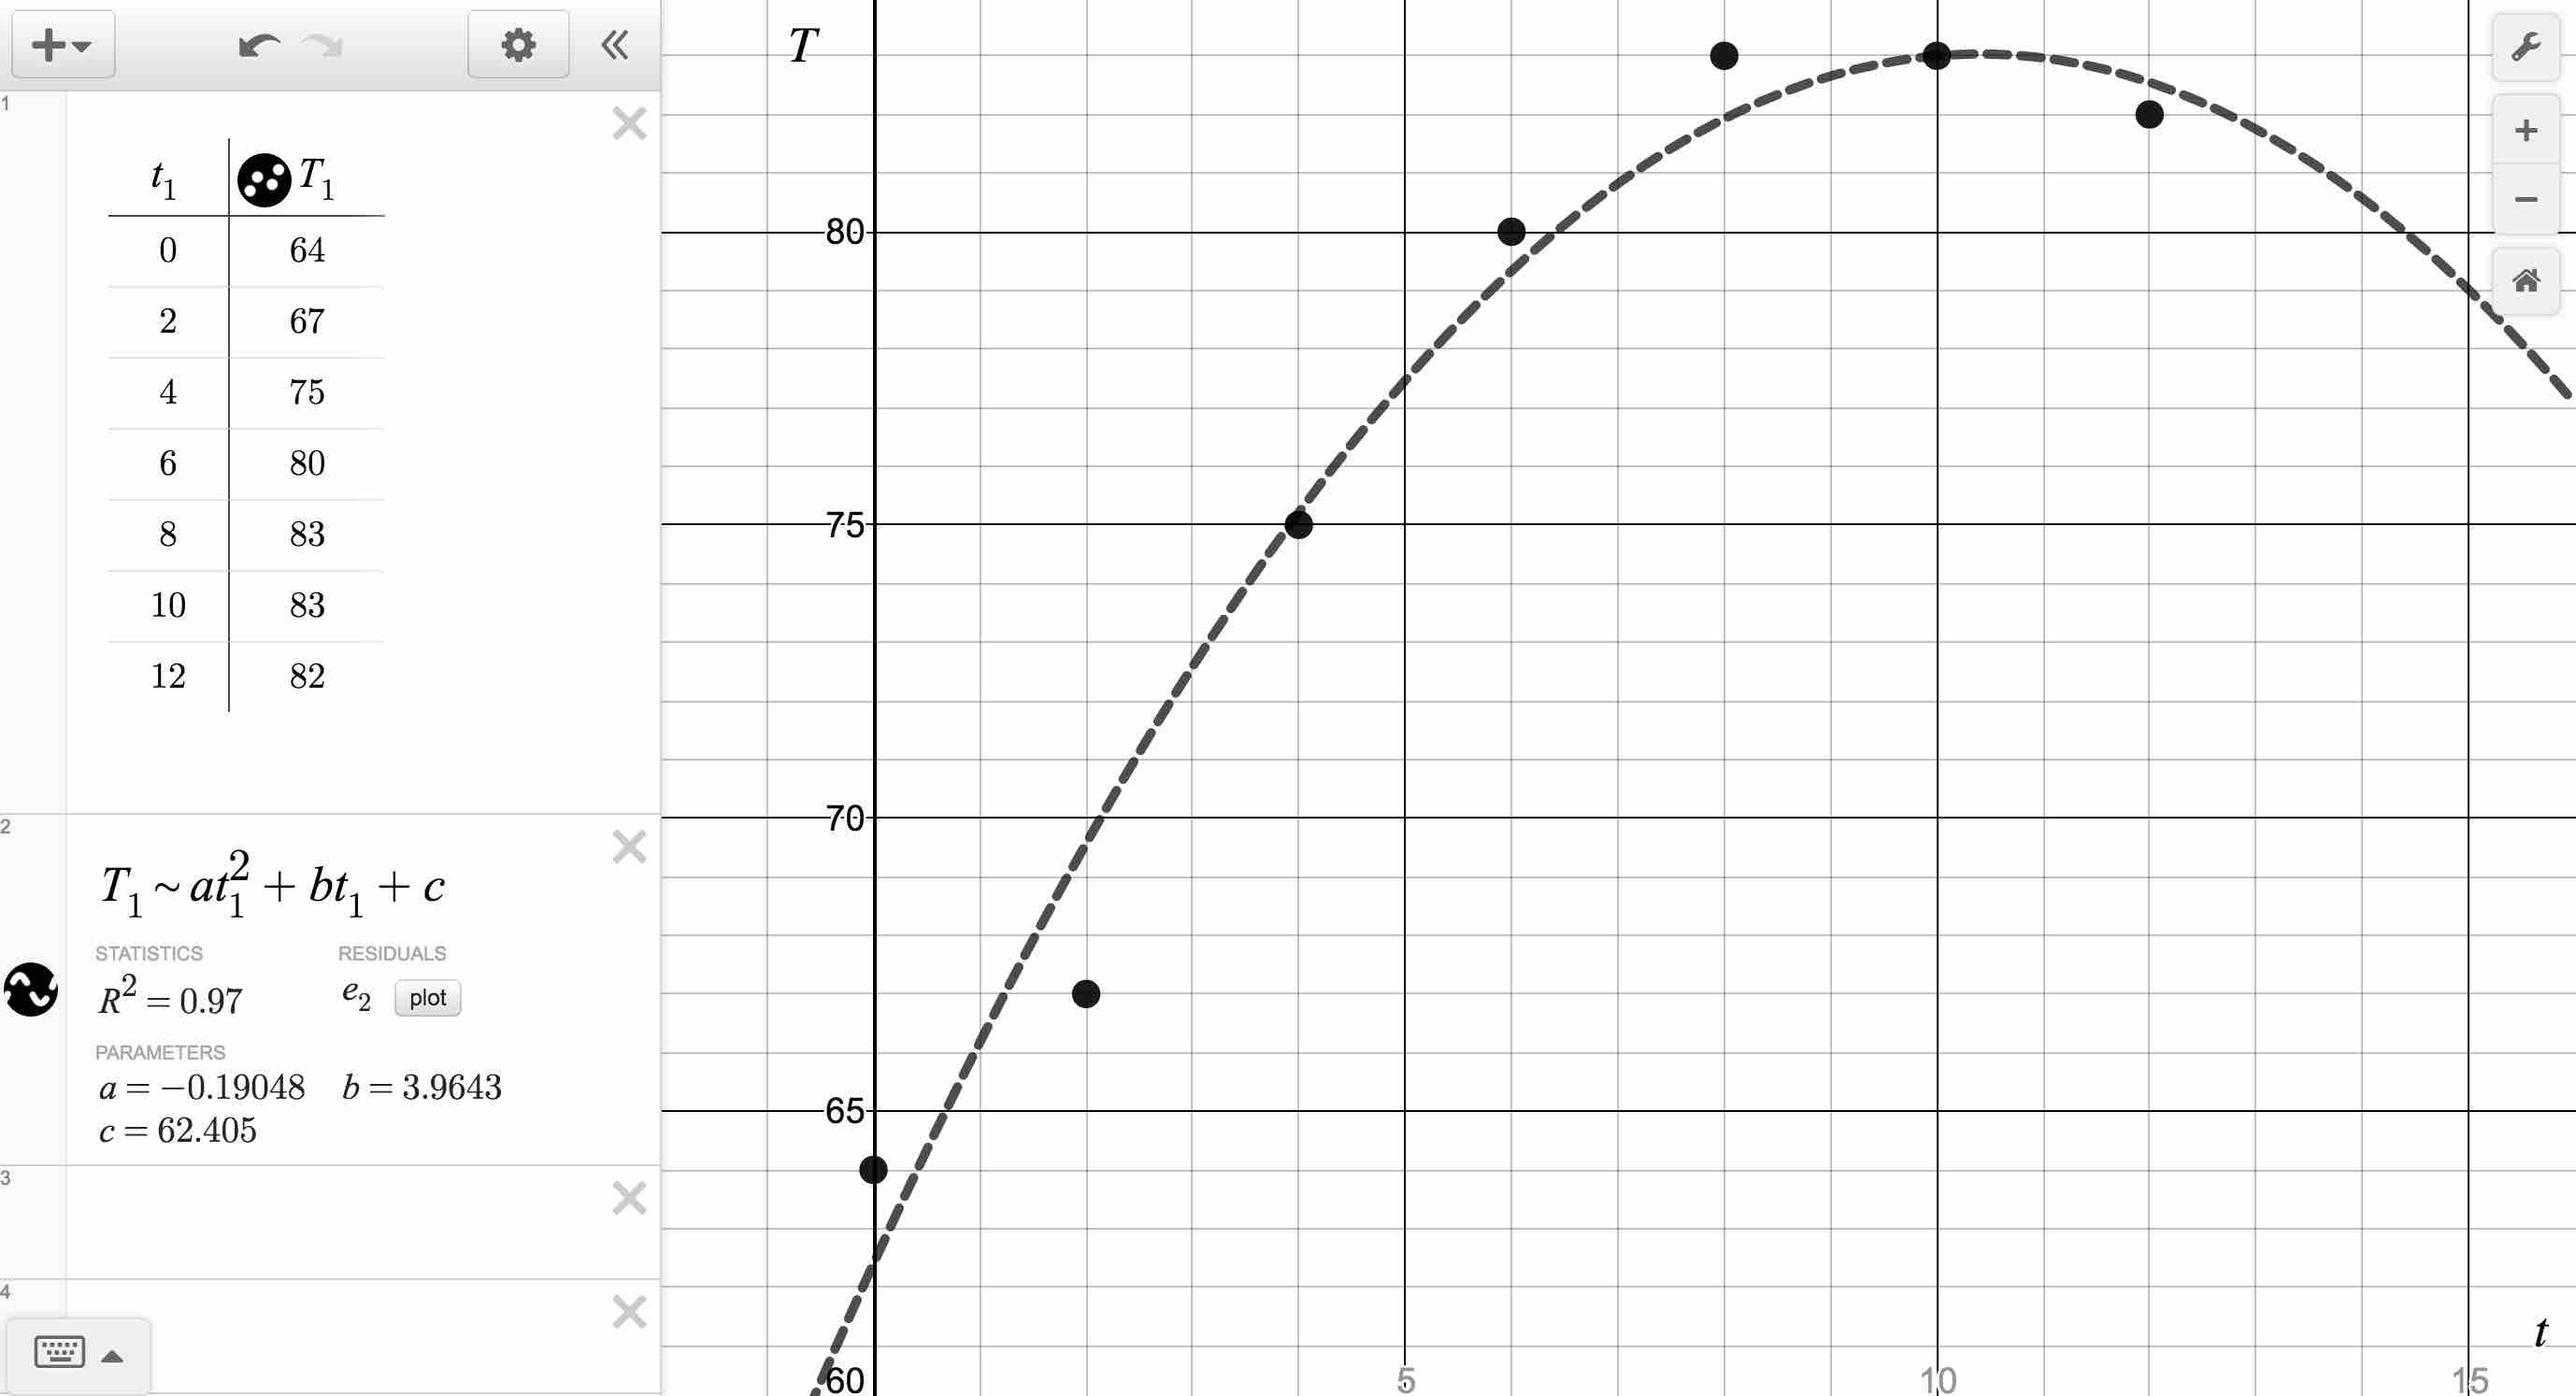
\includegraphics[width=5in]{./QuadraticFunctionsGraphics/TimeTempDataQR.jpg}
 
 \end{center}
 
 \qed
 
 \end{enumerate}
 
 \end{ex}

It is interesting how close the predictions from  Examples \ref{timetempregressionex} and  \ref{TimeTempQRex} despite one using linear models and one using a quadratic model.  Which model is the `better' model?  We leave that discussion to the reader and their classmates.

\medskip

Our next example is classic application of optimizing a quadratic function.

\begin{ex} \label{donniealpaca} Much to Donnie's surprise and delight, he inherits a large parcel of land in Ashtabula County from one of his (e)strange(d) relatives so the time is right for him to pursue his dream of raising alpaca.  He wishes to build a rectangular pasture and estimates that he has enough money for 200 linear feet of fencing material.  If he makes the pasture adjacent to a river (so that no fencing is required on that side), what are the dimensions of the pasture which maximize the area?  What is the maximum area?  If an average alpaca needs 25 square feet of grazing area, how many alpaca can Donnie keep in his pasture?

\pagebreak

{\bf Solution.} We are asked to find the dimensions of the pasture which would give a maximum area, so we begin by sketching the diagram seen below on the left.  We let $w$ denote the width of the pasture and we let $\ell$ denote the length of the pasture.  The units given to us in the statement of the problem are feet, so we assume that $w$ and $\ell$ are measured in feet.  The area of the pasture, which we'll call $A$, is related to $w$ and $\ell$ by the equation $A = w \ell$.  Since $w$ and $\ell$ are both measured in feet, $A$ has units of $\text{feet}^2$, or square feet.  

\medskip

We are also told that the total amount of fencing available is $200$ feet, which means $w + \ell + w = 200$, or, $\ell+2w = 200$.  We now have two equations, $A = w \ell$ and $\ell+2w = 200$.  In order to use the tools given to us in this section to \textit{maximize} $A$, we need to use the information given to write $A$ as a function of just \textit{one} variable, either $w$ or $\ell$. This is where we use the equation $\ell+2w = 200$.  Solving for $\ell$, we find $\ell = 200-2w$, and we substitute this into our equation for $A$.  We get $A = w \ell = w(200-2w) = 200w-2w^2$.  We now have $A$ as a function of $w$, $A = f(w) = 200w-2w^2 = -2w^2+200w$. 

\begin{center}

\setlength\columnsep{0pt}

\begin{multicols}{2}

\begin{mfpic}[15]{-4}{4}{0}{4}
\fillcolor[gray]{0.8}
\gfill \rect{(-4,2), (4,4)}

\dashed \polyline{(-3,2), (-3,0.5), (3,0.5), (3,2)}
\tlabel[cc](-3.5,1.25){$w$}
\tlabel[cc](0,0){$\ell$}
\tlabel[cc](3.5, 1.25){$w$}
\tlabel[cc](0,1.25){pasture}
\tlabel[cc](0,3){river} 

\penwd{1.25pt}
\polyline{(-4,2), (4,2)}
\polyline{(-4,4), (4,4)}


\end{mfpic}

\begin{mfpic}[15]{-1}{10.75}{-1}{6}
\axes
\tlabel[cc](11,0){\scriptsize  $w$}
\tlabel[cc](0.5,6){\scriptsize  $A$}
\tlabel[cc](5,5.5){\scriptsize  $(50, 5000)$}
\tlabel[cc](-0.75,-0.5){\scriptsize  $(0, 0)$}
\tlabel[cc](10,-0.5){\scriptsize $(100, 0)$}
\tlabel[cc](5,5.5){\scriptsize  $(50, 5000)$}
\tcaption{\scriptsize $A = f(w)$}
\xmarks{1 step 1 until 10}
\ymarks{1 step 1 until 5}
\scriptsize
\tlpointsep{4pt}
\axislabels {x}{ {$10$} 1, {$30$} 3,  {$50$} 5,{$70$} 7}
\axislabels {y}{{$1000$} 1, {$2000$} 2, {$3000$} 3, {$4000$} 4, {$5000$} 5}
\normalsize
\penwd{1.25pt}
\function{0,10,0.1}{(0-0.2)*(x**2) + 2*x}
\point[4pt]{(5,5)}
\pointfillfalse
\point[4pt]{(0,0), (10,0)}

\end{mfpic}

\end{multicols}

\setlength\columnsep{10pt}

\end{center}

Before we go any further, we need to find the applied domain of $f$ so that we know what values of $w$ make sense in this situation.\footnote{Donnie would be very upset if, for example, we told him the width of the pasture needs to be $-50$ feet.}  Given that $w$ represents the width of the pasture we need $w > 0$.  Likewise, $\ell$ represents the length of the pasture, so $\ell = 200-2w > 0$.  Solving this latter inequality yields $w < 100$.  Hence, the function we wish to maximize is $f(w) = -2w^2 + 200w$ for $0 < w < 100$.  We know two things about the quadratic function $f$: the graph of $A = f(w)$ is a parabola and (since the coefficient of $w^2$ is $-2$) the parabola opens downwards.  

\medskip

This means that there is a maximum value to be found, and we know it occurs at the vertex.  Using the vertex formula, we find $w = -\frac{200}{2(-2)} = 50$, and $A = f(50) = -2(50)^2 + 200(50) = 5000$.  Since $w=50$ lies in the applied domain, $0 < w < 100$, we have that the area of the pasture is maximized when the width is $50$ feet.  To find the length, we use $\ell = 200-2w$ and find $ \ell = 200-2(50) = 100$, so the length of the pasture is $100$ feet.  The maximum area is $A =f(50) = 5000$, or $5000$ square feet.  If an average alpaca requires 25 square feet of pasture, Donnie can raise $\frac{5000}{25} = 200$ average alpaca. \qed

\end{ex}

The function $f$ in Example \ref{donniealpaca} is called the\index{objective function}\index{optimization ! objective function} \textbf{objective function} for this problem - it's the function we're trying to optimize.  In the case above, we were trying to maximize $f$. The equation  $\ell+2w = 200$ along with the inequalities $w>0$ and $\ell >0$ are called the\index{constraint}\index{optimization ! constraint} \textbf{constraints}.   As we saw in this example, and as we'll see again and again, the constraint equation is used to rewrite the objective function in terms of just one of the variables where constraint inequalities, if any, help determine the applied domain.

\subsection{Inequalities involving Quadratic Functions}
\label{QuadraticInequalities}


We now turn our attention to solving inequalities involving quadratic functions.   Consider the inequality $x^2 \leq 6$.  We could use the fact that the square root is increasing\footnote{That is, if $a < b$, then $\sqrt{a} < \sqrt{b}$.} to get: $\sqrt{x^2} \leq \sqrt{6}$, or $|x| \leq \sqrt{6}$.  This reduces to $-\sqrt{6} \leq x \leq \sqrt{6}$ or, using interval notation, $[-\sqrt{6}, \sqrt{6}]$. If, however, we had to solve $x^2 \leq x+6$, things are more complicated.  One approach is to complete the square: \[ \begin{array}{rcl}

x^2 & \leq & x+6 \\
x^2 - x & \leq & 6 \\
x^2 - x + \frac{1}{4} & \leq &  6 + \frac{1}{4} \\ [3pt]

\left(x - \frac{1}{2} \right)^2 & \leq & \frac{25}{4} \\ [3pt]

\sqrt{\left(x - \frac{1}{2} \right)^2} & \leq & \sqrt{\frac{25}{4}} \\ [3pt]

\left| x - \frac{1}{2} \right| & \leq & \frac{5}{2} \\ 

-\frac{5}{2} \quad \leq & x - \frac{1}{2} & \leq \quad \frac{5}{2} \\ 

-2 \quad &  \leq  x  \leq & 3 \\  \end{array} \] We get the solution $[-2,3]$.  While there is nothing wrong with this approach, we seek methods here that will generalize to higher degree polynomials such as those we'll see in Chapter \ref{PolynomialFunctions}.  

\medskip

To that end, we look at the inequality $x^2 \leq x+6$ graphically.  Identifying $f(x) = x^2$ and $g(x) = x+6$ , we graph $f$ and $g$ on the same set of axes below on the left and look for where the graph of $f$ (the parabola) meets or is below the graph of $g$ (the line).  There are two points of intersection which we determine by solving  $f(x) = g(x)$ or $x^2=x+6$.  As usual, we rewrite this equation as $x^2-x-6 = 0$ in order to use the primary tools we've developed to handle these types\footnote{Namely ones with a nonzero coefficient of `$x$'.} of quadratic equations: factoring, or failing that, the Quadratic Formula.  We find $x^2-x-6 = (x+2)(x-3)$ so we get two solutions to $(x+2)(x-3) = 0$, namely $x = -2$ and $x = 3$.  Putting these together with the graph, we obtain the same solution:  $[-2,3]$.  

\begin{center}

\begin{multicols}{2}

\begin{mfpic}[15]{-4}{4}{-1}{10}
\axes
\tlabel[cc](4,-0.5){\scriptsize $x$}
\tlabel[cc](0.5,10){\scriptsize $y$}
\xmarks{-3 step 1 until 3}
\ymarks{1 step 1 until 9}
\scriptsize
\tlabel[cc](-3,4){\scriptsize $(-2,4)$}
\tlabel[cc](4,9){\scriptsize $(3,9)$}
\tlpointsep{4pt}
\axislabels {x}{{$-3 \hspace{7pt}$} -3, {$-2 \hspace{7pt}$} -2, {$-1 \hspace{7pt}$} -1, {$1$} 1, {$2$} 2, {$3$} 3}
\axislabels {y}{{$1$} 1, {$2$} 2, {$3$} 3, {$4$} 4, {$5$} 5, {$6$} 6, {$7$} 7, {$8$} 8, {$9$} 9}
\tcaption{\scriptsize Solving $x^2 \leq x+6$.}
\normalsize
\arrow \reverse \arrow \function{-3.15,3.15,0.1}{x**2}
\arrow \reverse \arrow \polyline{(-4,2), (4,10)}
\penwd{1.25pt}
\function{-2,3,0.1}{x**2}
\polyline{(-2,4), (3,9)}
\point[4pt]{(-2,0),(3,0), (-2,4), (3,9)}
\polyline{(-2,0), (3,0)}
\end{mfpic}


\begin{mfpic}[11.78]{-4}{4}{-7}{7}
\axes
\tlabel[cc](4,-0.5){\scriptsize $x$}
\tlabel[cc](0.5,7){\scriptsize $y$}
\tlabel[cc](-3.5,0.5){\scriptsize $(-2,0)$}
\tlabel[cc](2,0.5){\scriptsize $(3,0)$}
\xmarks{-3 step 1 until 3}
\ymarks{-5 step 1 until 6}
\scriptsize
\tlpointsep{4pt}
\axislabels {x}{{$-3 \hspace{7pt}$} -3,  {$-1 \hspace{7pt}$} -1, {$1$} 1, {$2$} 2}
\axislabels {y}{{$-6$} -6,  {$-4$} -4,{$-2$} -2,   {$2$} 2, {$4$} 4,  {$6$} 6}
\tcaption{\scriptsize Solving $x^2-x-6 \leq 0$.}
\normalsize
\arrow \reverse \arrow \function{-3,4,0.1}{x**2-x-6}
\penwd{1.25pt}
\function{-2,3,0.1}{x**2-x-6}
\polyline{(-2,0), (3,0)}
\point[4pt]{(-2,0),(3,0)}
\end{mfpic}

\end{multicols}

\end{center}

Yet a third way to attack $x^2 \leq x+6$ is to rewrite the inequality as $x^2-x-6 \leq 0$.  Here, we graph $f(x) = x^2-x-6$ to look for where the graph meets or is below the graph of $g(x) = 0$, a.k.a. the $x$-axis.  Doing so requires us to find the zeros of $f$, that is, solve $f(x) = x^2-x-6=0$ from which we obtain $x =-2$ and $x = 3$ as before.  We find the same solution, $[-2,3]$ as is showcased in the graph at the bottom of the previous page on the right.  

\medskip

One advantage to using this last approach is that we are essentially concerned with \text{one} function and its \textit{zeros}.  This approach can be generalized to all functions - not just quadratics, so we take the time to develop this method more thoroughly now.  

\phantomsection
\label{firstsigndiagram}

\medskip

Consider the graph of $f(x) = x^2-x-6$ below  The zeros of $f$ are $x=-2$ and $x=3$ and they divide the domain (the $x$-axis) into three intervals:  $(-\infty, -2)$, $(-2,3)$ and $(3, \infty)$.  For every number in $(-\infty, -2)$, the graph of $f$ is above the $x$-axis; in other words, $f(x) > 0$ for all $x$ in $(-\infty, -2)$. Similarly, $f(x) < 0$ for all $x$ in $(-2,3)$, and $f(x) > 0$ for all $x$ in $(3, \infty)$.  We represent this schematically with the {\bf sign diagram} below.\index{inequality ! sign diagram}\index{sign diagram ! for quadratic inequality} 

\begin{center}

\begin{multicols}{2}

\begin{mfpic}[12]{-4}{4}{-7}{7}
\axes
\tlabel[cc](4,-0.5){\scriptsize $x$}
\tlabel[cc](0.5,7){\scriptsize $y$}
\tlabel[cc](-3.5,0.5){\scriptsize $(-2,0)$}
\tlabel[cc](2,0.5){\scriptsize $(3,0)$}
\xmarks{-3 step 1 until 3}
\ymarks{-5 step 1 until 6}
\scriptsize
\tlpointsep{4pt}
\axislabels {x}{{$-3 \hspace{7pt}$} -3,  {$-1 \hspace{7pt}$} -1, {$1$} 1, {$2$} 2}
\axislabels {y}{{$-6$} -6,  {$-4$} -4,{$-2$} -2,   {$2$} 2, {$4$} 4,  {$6$} 6}
\tcaption{ $f(x) = x^2-x-6$.}
\normalsize
\penwd{1.25pt}
\arrow \reverse \arrow \function{-3,4,0.1}{x**2-x-6}
\point[4pt]{(-2,0),(3,0)}
\end{mfpic} 

\columnbreak

\vspace*{0.75in}
\begin{mfpic}[15]{-5}{5}{-5}{6}
\arrow \reverse \arrow \polyline{(-5,0),(5,0)}
\xmarks{-2,2}
\tcaption{A sign diagram for $f(x) = x^2-x-6$}
\tlpointsep{4pt}
\axislabels {x}{{$-2 \hspace{7pt}$} -2, {$3$} 2}
\tlabel[cc](-3.5,1){$(+)$}
\tlabel[cc](-2,1){$0$}
\tlabel[cc](0,1){$(-)$}
\tlabel[cc](2,1){$0$}
\tlabel[cc](3.5,1){$(+)$}
\end{mfpic}

\end{multicols}

\end{center}

The $(+)$ above a portion of the number line indicates $f(x) > 0$ for those values of $x$ and the $(-)$ indicates $f(x) < 0$ there.  The numbers labeled on the number line are the zeros of $f$, so we place $0$ above them.  For the inequality $f(x) = x^2-x-6 \leq 0$, we read from the sign diagram that the solution is $[-2,3]$.  

\medskip

Our next goal is to establish a procedure by which we can generate the sign diagram without graphing the function.  While parabolas aren't that bad to graph knowing what we know, our sights are set on more general functions whose graphs are more complicated.  

\medskip
\enlargethispage{.in}

An important property of parabolas is that a parabola can't be above the $x$-axis at one point and below the $x$-axis at another point without crossing the $x$-axis at some point in between. Said differently, if the function is positive at one point and negative at another, the function must have at least one zero in between.  This property is a consequence of quadratic functions being\index{function ! continuous}\index{continuous} \textbf{continuous}.  A precise definition of `continuous' requires the language of Calculus, but it suffices for us to know that the graph of a continuous function has no gaps or holes.   This allows us to determine the sign of \emph{all} of the function values on a given interval by testing the function at just \emph{one} value in the interval.  

\medskip

The result below applies to all continuous functions defined on an interval of real numbers, but we restrict our attention to quadratic functions for the time being,

\medskip

\colorbox{ResultColor}{\bbm

\centerline{\textbf{Steps for Creating A Sign Diagram for A Quadratic Function}} \index{sign diagram ! creating }

\smallskip

Suppose $f$ is a quadratic function.

\begin{enumerate}

\item  Find the zeros of $f$ and place them on the number line with the number $0$ above them.

\item  Choose a real number, called a \textbf{test value}, in each of the intervals determined in step 1. 

\item  Determine and record the sign of $f(x)$ for each test value in step 2.

\end{enumerate}

\ebm}

\medskip

To use a sign diagram to solve an inequality, we must always remember to compare the function to $0$.

\medskip

\colorbox{ResultColor}{\bbm

\centerline{\textbf{Solving Inequalities using Sign Diagrams}} \index{inequality ! solution using sign diagram }

\smallskip

To solve an inequality using a sign diagram:

\begin{enumerate}

\item  Rewrite the inequality so some function $f(x)$ is being compared to `$0$.'

\item  Make a sign diagram for $f$.

\item  Record the solution.

\end{enumerate}

\ebm}

\medskip

We practice this approach in the following example.

\begin{ex}  Solve the following inequalities analytically\footnote{By `solve analytically' we mean `algebraically' using a sign diagram.} and check your solutions graphically.

\begin{multicols}{2}
\begin{enumerate}

\item  $2x^2 \leq 3-x$

\item  $t^2 - 2t > 1$

\setcounter{HW}{\value{enumi}}
\end{enumerate}
\end{multicols}

\begin{multicols}{2}
\begin{enumerate}
\setcounter{enumi}{\value{HW}}

\item  $x^2+1 \leq 2x$

\item  $2t-t^2 \geq |t-1|-1$

\end{enumerate}
\end{multicols}

{\bf Solution.}  

\begin{enumerate}

\item  To solve $2x^2 \leq 3-x$, we rewrite it as $2x^2+x-3 \leq 0$.  We find the zeros of $f(x) = 2x^2 + x - 3$ by solving $2x^2 + x - 3 = 0$.  Factoring gives $(2x+3)(x-1)=0$, so $x = -\frac{3}{2}$ or $x = 1$.  We place these values on the number line with $0$ above them and choose test values in the intervals $\left(-\infty, -\frac{3}{2}\right)$, $\left(-\frac{3}{2},1\right)$ and $(1,\infty)$.  For the interval  $\left(-\infty, -\frac{3}{2}\right)$, we choose\footnote{We have to choose \textit{something} in each interval.  If you don't like our choices, please feel free to choose different numbers.  You'll get the same sign chart.} $x=-2$; for $\left(-\frac{3}{2},1\right)$, we pick $x=0$; and for $(1,\infty)$, $x=2$. Evaluating the function at the three test values gives us $f(-2) = 3 > 0$, so we place $(+)$ above $\left(-\infty, -\frac{3}{2}\right)$;  $f(0)=-3 < 0$, so $(-)$ goes above the interval $\left(-\frac{3}{2},1\right)$;  and, $f(2) = 7$, which means $(+)$ is placed above $(1,\infty)$.

\medskip

We are solving $2x^2+x-3 \leq 0$ so we need solutions to $2x^2+x-3 < 0$ as well as solutions for $2x^2+x-3 =0$.  For $2x^2+x-3 < 0$, we need the intervals which we have a $(-)$ above them.  The sign diagram shows only one: $\left(-\frac{3}{2},1\right)$.  Also, we know $2x^2+x-3 =0$ when $x=-\frac{3}{2}$ and $x=1$, so our final answer is $\left[-\frac{3}{2},1\right]$.  

\medskip

To verify our solution graphically, we refer to the original inequality, $2x^2 \leq 3-x$.  We let $g(x) = 2x^2$ and $h(x)=3-x$.  We are looking for the $x$ values where the graph of $g$ is below that of $h$ (the solution to $g(x) < h(x)$) as well as the points of intersection (the solutions to $g(x)=h(x)$).  The graphs of $g$ and $h$ are given on the right with the sign chart on the left.


\begin{center}

\begin{multicols}{2}

\vspace*{.25in}

\begin{mfpic}[15]{-5}{5}{-2}{2}
\arrow \reverse \arrow \polyline{(-5,0),(5,0)}
\xmarks{-2,2}
\arrow \polyline{(-3.5,-1.5),(-3.5,-0.5)}
\arrow \polyline{(0,-1.5),(0,-0.5)}
\arrow \polyline{(3.5,-1.5),(3.5,-0.5)}
\tlpointsep{4pt}
%\scriptsize
\axislabels {x}{{$-\frac{3}{2} \hspace{7pt}$} -2, {$1$} 2}
\tlabel[cc](-3.5,1){$(+)$}
\tlabel[cc](-2,1){$0$}
\tlabel[cc](0,1){$(-)$}
\tlabel[cc](2,1){$0$}
\tlabel[cc](3.5,1){$(+)$}
\tlabel[cc](-3.75,-2.25){$-2$}
\tlabel[cc](-0.1,-2.25){$0$}
\tlabel[cc](3.4,-2.25){$2$}
%\normalsize
\end{mfpic}  

\columnbreak

\begin{mfpic}[20][10]{-3}{3}{-1}{8}
\arrow \reverse \arrow \function{-2,2,0.1}{2*(x**2)}
\arrow \reverse \arrow \polyline{(-3,6),(2.5,0.5)}
\xmarks{-2 step 1 until 2}
\ymarks{1 step 1 until 7}
\axes
\tlabel[cc](3,-0.5){\scriptsize $x$}
\tlabel[cc](0.5,8){\scriptsize $y$}
\tlabel[cc](2.75,6){\scriptsize $y=2x^2$}
\tlabel[cc](3,1.75){\scriptsize $y=3-x$}
\scriptsize
\tlpointsep{4pt}
\axislabels {x}{{$-2 \hspace{7pt}$} -2, {$-1 \hspace{7pt}$} -1,{$1$} 1, {$2$} 2}
\axislabels {y}{{$2$} 2, {$3$} 3, {$4$} 4, {$5$} 5, {$6$} 6, {$7$} 7}
\normalsize 
\penwd{1.25pt} 
 \function{-1.5,1,0.1}{2*(x**2)}
 \polyline{(-1.5,4.5),(1,2)}
\polyline{(-1.5,0), (1,0)}
\point[4pt]{(-1.5,0), (1,0), (-1.5, 4.5), (1,2)}
\end{mfpic}

\end{multicols}

\end{center}

\item Once again, we re-write  $t^2-2t > 1$ as $t^2-2t-1>0$ and we identify $f(t)=t^2-2t-1$.  When we go to find the zeros of $f$, we find, to our chagrin, that the quadratic $t^2-2t-1$ doesn't factor nicely.  Hence, we resort to  the Quadratic Formula and find $t=1 \pm \sqrt{2}$.  As before, these zeros divide the number line into three pieces.  To help us decide on test values, we approximate $1 - \sqrt{2} \approx -0.4$ and $1 + \sqrt{2} \approx 2.4$.  We choose $t=-1$, $t=0$ and $t=3$ as our test values and find $f(-1)= 2$, which is $(+)$; $f(0)=-1$ which is $(-)$; and $f(3)=2$ which is $(+)$ again.  Our solution to $t^2-2t-1>0$ is where we have $(+)$, so, in interval notation $\left(-\infty, 1-\sqrt{2}\right) \cup \left(1+\sqrt{2},\infty\right)$.  

\medskip

To check the inequality $t^2 - 2t > 1$ graphically, we set $g(t) = t^2-2t$ and $h(t)=1$.  We are looking for the $t$ values where the graph of $g$ is above the graph of $h$.  As before we present the graphs on the right and the sign chart on the left.

\begin{center}

\begin{multicols}{2}

\vspace*{.25in}

\begin{mfpic}[14]{-8}{8}{-2}{2}
\arrow \reverse \arrow \polyline{(-8,0),(8,0)}
\xmarks{-3,3}
\arrow \polyline{(-6,-1.5),(-6,-0.5)}
\arrow \polyline{(0,-1.5),(0,-0.5)}
\arrow \polyline{(6,-1.5),(6,-0.5)}
\tlpointsep{4pt}
%\scriptsize
\axislabels {x}{{$1-\sqrt{2}$} -3, {$1+\sqrt{2}$} 3}
\tlabel[cc](-6,1){$(+)$}
\tlabel[cc](-3,1){$0$}
\tlabel[cc](0,1){$(-)$}
\tlabel[cc](3,1){$0$}
\tlabel[cc](6,1){$(+)$}
\tlabel[cc](-6,-2.25){$-1$}
\tlabel[cc](0,-2.25){$0$}
\tlabel[cc](6,-2.25){$3$}
%\normalsize
\end{mfpic} 

\columnbreak

\begin{mfpic}[20]{-4}{4}{-1}{4}
\arrow \reverse \arrow \function{-1.23,3.21,0.1}{(x**2)-2*x}
\arrow \reverse \arrow \function{-4,4,0.1}{1}
\xmarks{-3 step 1 until 3}
\ymarks{1 step 1 until 3}
\axes
\tlabel[cc](4,-0.5){\scriptsize $t$}
\tlabel[cc](0.5,4){\scriptsize $y$}
\tlabel[cc](-2.5,1.25){\scriptsize $y=1$}
\tlabel[cc](2.75,-1){\scriptsize $y=t^2-2t$}
\scriptsize
\tlpointsep{4pt}
\axislabels {x}{{$-3 \hspace{7pt}$} -3,{$-2 \hspace{7pt}$} -2,{$-1 \hspace{7pt}$} -1,{$1$} 1, {$2$} 2, {$3$} 3}
\axislabels {y}{{$2$} 2, {$3$} 3}
\normalsize 
\penwd{1.25pt} 
\arrow \reverse \function{-1.23,-0.4142,0.1}{(x**2)-2*x}
\arrow \function{2.4142,3.21,0.1}{(x**2)-2*x}
\arrow \polyline{(-0.4142,0), (-4,0)}
\arrow \polyline{(2.4142,0), (4,0)}
\arrow \polyline{(-0.4142,1), (-4,1)}
\arrow \polyline{(2.4142,1), (4,1)}
\pointfillfalse
\point[4pt]{(-0.4142,0),(2.4142,0)}
\point[4pt]{(-0.4142,1),(2.4142,1)}
\end{mfpic}

\end{multicols}

\end{center}


\item  To solve  $x^2+1 \leq 2x$, as before, we solve  $x^2-2x+1 \leq 0$.  Setting $f(x) = x^2-2x+1=0$, we find only one zero of $f$: $x = 1$.  This one $x$ value divides the number line into two intervals, from which we choose $x=0$ and $x=2$ as test values.  We find $f(0)=1 > 0$ and $f(2) = 1 > 0$.  Since we are looking for solutions to $x^2-2x+1 \leq 0$, we are looking for $x$ values where $x^2-2x+1 < 0$ as well as where $x^2-2x+1 = 0$.  Looking at our sign diagram, there are no places where $x^2-2x+1 < 0$ (there are no $(-)$), so our solution is only $x=1$ (where $x^2-2x+1 = 0$).  We write this as $\left\{1\right\}$.  

\medskip

Graphically, we solve $x^2+1 \leq 2x$ by graphing $g(x) = x^2+1$ and $h(x)=2x$. We are looking for the $x$ values where the graph of $g$ is below the graph of $h$ (for $x^2+1 < 2x$) and where the two graphs intersect ($x^2+1 = 2x$).  Notice that the line and the parabola touch at $\left(1, 2\right)$, but the parabola is always above the line otherwise.\footnote{In this case, we say the line $y=2x$ is \textbf{tangent} to $y=x^2+1$ at $\left(1, 2\right)$.  Finding tangent lines to arbitrary functions is a fundamental problem solved, in general, with Calculus.}

\begin{center}

\begin{multicols}{2}

\vspace*{.25in}

\begin{mfpic}[15]{-5}{5}{-2}{2}
\arrow \reverse \arrow \polyline{(-5,0),(5,0)}
\xmarks{0}
\arrow \polyline{(-2.5,-1.5),(-2.5,-0.5)}
\arrow \polyline{(2.5,-1.5),(2.5,-0.5)}
\tlpointsep{4pt}
%\scriptsize
\axislabels {x}{{$1$} 0}
\tlabel[cc](-2.5,1){$(+)$}
\tlabel[cc](0,1){$0$}
\tlabel[cc](2.5,1){$(+)$}
\tlabel[cc](-2.6,-2.1){$0$}
\tlabel[cc](2.4,-2.1){$2$}
%\normalsize
\end{mfpic}  

\columnbreak

\begin{mfpic}[20]{-2}{2}{-1}{5}
\arrow \reverse \arrow \function{-2,2,0.1}{(x**2)+1}
\arrow \reverse \arrow \function{-0.5,2.5,0.1}{2*x}
\point[4pt]{(1,2), (1,0)}
\xmarks{-1 step 1 until 1}
\ymarks{1 step 1 until 4}
\axes
\tlabel[cc](2,-0.5){\scriptsize $x$}
\tlabel[cc](0.5,5){\scriptsize $y$}
\tlabel[cc](1,0.5){\scriptsize $y=2x$}
\tlabel[cc](-2.25,2){\scriptsize $y=x^2+1$}
\scriptsize
\tlpointsep{4pt}
\axislabels {x}{{$-1 \hspace{7pt}$} -1,{$1$} 1}
\axislabels {y}{{$1$} 1,{$2$} 2, {$3$} 3, {$4$} 4}
\normalsize 
\end{mfpic}

\end{multicols}

\end{center}

\item  To solve $2t-t^2 \geq |t-1|-1$ analytically we first rewrite the absolute value using cases.  For $t< 1$, $|t-1| = -(t-1) = -t+1$, so we get $2t-t^2 \geq (-t+1)-1$ which simplifies to  $t^2-3t \leq 0$.  Finding the zeros of $f(t) = t^2-3t$, we get $t=0$ and $t=3$.  However, we are concerned only with the portion of the number line where $t < 1$, so the only zero that we deal with is $t=0$.  This divides the interval $t<1$ into two intervals:  $(-\infty, 0)$ and $(0,1)$.  We choose $t=-1$ and $t=\frac{1}{2}$ as our test values.  We find $f(-1) = 4$ and $f\left(\frac{1}{2}\right) = -\frac{5}{4}$.  Hence, our solution to $t^2-3t \leq 0$ for $t < 1$ is $[0,1)$. 

 Next, we turn our attention to the case $t \geq 1$.  Here, $|t-1| = t-1$, so our original inequality becomes $2t-t^2 \geq (t-1)-1$, or $t^2-t-2 \leq 0$.  Setting $g(t) = t^2-t-2$, we find the zeros of $g$ to be $t=-1$ and $t=2$.  Of these, only $t=2$ lies in the region $t\geq 1$, so we ignore $t=-1$.  Our test intervals are now $[1,2)$ and $(2,\infty)$.  We choose $t=1$ and $t=3$ as our test values and find $g(1) = -2$ and $g(3) = 4$.  Hence, our solution to $g(t) = t^2-t-2 \leq 0$, in this region is $[1,2)$.

\begin{center}

\begin{multicols}{2}

\begin{mfpic}[15]{-5}{5.5}{-2}{2}
\arrow \reverse \polyline{(-5,0),(5,0)}
\xmarks{0}
\arrow \polyline{(-2.5,-1.5),(-2.5,-0.5)}
\arrow \polyline{(2.5,-1.25),(2.5,-0.5)}
\tlpointsep{4pt}
%\scriptsize
\axislabels {x}{{$0$} 0}
\tlabel[cc](-2.5,1){$(+)$}
\tlabel[cc](0,1){$0$}
\tlabel[cc](2.5,1){$(-)$}
\tlabel[cc](-2.5,-2.25){$-1$}
\tlabel[cc](2.5,-2.25){$\frac{1}{2}$}
\gclear \circle{(5,0),0.2}
\circle{(5,0),0.2}
\tlabel[cc](5,-0.75){$1$}
%\normalsize
\end{mfpic}  

Solving $2t-t^2 \geq |t-1|-1$ for $t < 1$. 

\columnbreak

\begin{mfpic}[15]{-5}{5.5}{-2}{2}
\arrow \polyline{(-5,0),(5,0)}
\xmarks{0}
\arrow \polyline{(-5,-1.5),(-5,-0.5)}
\arrow \polyline{(2.5,-1.5),(2.5,-0.5)}
\tlpointsep{4pt}
%\scriptsize
\axislabels {x}{{$2$} 0}
\tlabel[cc](-2.5,1){$(-)$}
\tlabel[cc](0,1){$0$}
\tlabel[cc](2.5,1){$(+)$}
\tlabel[cc](2.5,-2.25){$3$}
\gfill \circle{(-5,0),0.2}
\tlabel[cc](-5,-2.25){$1$}
%\normalsize
\end{mfpic} 

Solving $2t-t^2 \geq |t-1|-1$ for $t \geq 1$.  

\end{multicols}

\end{center}

Combining these into one sign diagram, we have that our solution is $[0,2]$.  Graphically, to check $2t-t^2 \geq |t-1|-1$, we set $h(t) = 2t-t^2$ and $i(t) = |t-1|-1$ and look for the $t$ values where the graph of $h$ intersects or is above the the graph of $i$ The combined sign chart is given on the left and the graphs are on the right.

\begin{center}

\begin{multicols}{2} \raggedcolumns

\vspace*{.35in}

\begin{mfpic}[15]{-5}{5}{-2}{2}
\arrow \reverse \arrow \polyline{(-5,0),(5,0)}
\xmarks{-2,2}
\arrow \polyline{(-3.5,-1.5),(-3.5,-0.5)}
\arrow \polyline{(0,-1.5),(0,-0.5)}
\arrow \polyline{(3.75,-1.5),(3.75,-0.5)}
\tlpointsep{4pt}
%\scriptsize
\axislabels {x}{{$0$} -2, {$2$} 2}
\tlabel[cc](-3.5,1){$(+)$}
\tlabel[cc](-2,1){$0$}
\tlabel[cc](0,1){$(-)$}
\tlabel[cc](2,1){$0$}
\tlabel[cc](3.5,1){$(+)$}
\tlabel[cc](-3.55,-2.25){$-1$}
\tlabel[cc](-0.05,-2.25){$0$}
\tlabel[cc](3.7,-2.25){$3$}
%\normalsize
\end{mfpic} 

\columnbreak

\begin{mfpic}[30]{-2}{4}{-1}{2}
\arrow \reverse \arrow \function{-0.4,2.4,0.1}{(2*x)-(x**2)}
\arrow \reverse \arrow \polyline{(-1,1),(1,-1),(3,1)}
\point[4pt]{(0,0),(2,0)}
\xmarks{-1 step 1 until 3}
\ymarks{1}
\axes
\tlabel[cc](4,-0.5){\scriptsize $t$}
\tlabel[cc](0.5,2){\scriptsize $y$}
\tlabel[cc](1,1.25){\scriptsize $y=2t-t^2$}
\tlabel[cc](1,-1.25){\scriptsize $y=|t-1|-1$}
\scriptsize
\tlpointsep{4pt}
\axislabels {x}{{$-1 \hspace{7pt}$} -1,{$1$} 1, {$2$} 2, {$3$} 3}
\axislabels {y}{{$1$} 1}
\normalsize 
\penwd{1.25pt} 
\function{0,2,0.1}{(2*x)-(x**2)}
\polyline{(0,0),(1,-1),(2,0)}
\polyline{(0,0),(2,0)}
\end{mfpic}

\end{multicols}

\end{center}

\end{enumerate}

\end{ex}

\vspace{-.4in} \qed

\medskip

We end this section with an example that combines quadratic inequalities with piecewise functions. 

\begin{ex}  Rewrite  $g(x) = |x^2 - x - 6|$ as a piecewise function and graph.

\smallskip

{\bf Solution.}  Using the definition of absolute value, Definition \ref{absolutevaluepiecewise} and the sign diagram we constructed for $f(x) = x^2-x-6$ near the beginning of the subsection, we get: \small \[ \begin{array}{ccc} 

g(x) = |x^2-x-6| = \begin{mycases} 
      -(x^2-x-6) &  \text{if $(x^2-x-6) < 0$, } \\
      (x^2-x-6)  & \text{if $(x^2-x-6) \geq 0$.} \\
   \end{mycases} &
   
   \longrightarrow &
   
 g(x) = \begin{mycases} 
      -x^2+x+6 &  \text{if $-2 < x < 3$, } \\
   x^2-x-6  & \text{if $x \leq -2$ or $x \geq 3$.} \\
   \end{mycases} \\ \end{array} \]  \normalsize Going through the usual machinations results on the graph below on the right.  Compare it to the graph below on the left.  Notice anything? \[ \begin{array}{cc}

\begin{mfpic}[15][10]{-4}{4}{-7}{8}
\axes
\tlabel[cc](4,-0.5){\scriptsize $x$}
\tlabel[cc](0.5,8){\scriptsize $y$}
\xmarks{-3 step 1 until 3}
\ymarks{-5 step 1 until 7}
\tcaption{ \scriptsize $y=f(x) = x^2-x-6$}
\tlpointsep{4pt}
\axislabels {x}{{\scriptsize $-3 \hspace{7pt}$} -3, {\scriptsize $-1 \hspace{7pt}$} -1, {\scriptsize $1$} 1, {\scriptsize $2$} 2}
\axislabels {y}{{\scriptsize $-6$} -6, {\scriptsize $-5$} -5, {\scriptsize $-4$} -4,{\scriptsize $-3$} -3, {\scriptsize $-2$} -2, {\scriptsize $-1$} -1, {\scriptsize $1$} 1, {\scriptsize $2$} 2, {\scriptsize $3$} 3, {\scriptsize $4$} 4, {\scriptsize $5$} 5, {\scriptsize $6$} 6, {\scriptsize $7$} 7}
\penwd{1.25pt}
\arrow \reverse \arrow \function{-3.25,4.25,0.1}{x**2-x-6}
\point[4pt]{(-2,0),(3,0)}
\end{mfpic} & \hspace{1in}

\begin{mfpic}[15][10]{-4}{4}{-7}{8}
\axes
\tlabel[cc](4,-0.5){\scriptsize $x$}
\tlabel[cc](0.5,8){\scriptsize $y$}

\tcaption{ \scriptsize $y=g(x) = |x^2-x-6|$}
\xmarks{-3 step 1 until 3}
\ymarks{-6,-5,-4,-3,-2,-1,1,2,3,4,5,7}
\tlpointsep{4pt}
\axislabels {x}{{\scriptsize $-3 \hspace{7pt}$} -3, {\scriptsize $-2 \hspace{7pt}$} -2, {\scriptsize $-1 \hspace{7pt}$} -1, {\scriptsize $1$} 1, {\scriptsize $2$} 2, {\scriptsize $3$} 3}
\axislabels {y}{{\scriptsize $-6$} -6, {\scriptsize $-5$} -5, {\scriptsize $-4$} -4,{\scriptsize $-3$} -3, {\scriptsize $-2$} -2, {\scriptsize $-1$} -1, {\scriptsize $1$} 1, {\scriptsize $2$} 2, {\scriptsize $3$} 3, {\scriptsize $4$} 4, {\scriptsize $5$} 5, {\scriptsize $6$} 6, {\scriptsize $7$} 7}
\penwd{1.25pt}
\arrow \reverse \function{-3.25,-2,0.1}{x**2-x-6}
\function{-2,3,0.1}{6+x-x**2}
\arrow \function{3,4.25,0.1}{x**2-x-6}
\point[4pt]{(-2,0),(3,0)}
\end{mfpic} \\

\end{array}\] If we take a step back and look at the graphs of $f$ and $g$,  we notice that to obtain the graph of $g$ from the graph of  $f$, we reflect a \textit{portion} of the graph of $f$ about the $x$-axis.  In general, if $g(x) = |f(x)|$, then: \[ g(x) = |f(x)| = \begin{mycases} 
      -f(x) &  \text{if $f(x)  < 0$, } \\
     f(x)  & \text{if $f(x)  \geq 0$.} \\
   \end{mycases}  \]  The function $g$ is defined so that when $f(x)$ is negative (i.e., when its graph is below the $x$-axis), the graph of $g$ is the refection of the graph of $f$ across the $x$-axis.   This is a general method  to graph functions of the form $g(x) = |f(x)|$.  Indeed, the graph of $g(x) = |x|$ can be obtained by reflection the portion of the line $f(x) =x$ which is below the $x$-axis back above the $x$-axis creating the characteristic `$\vee$' shape.\footnote{See Exercise \ref{makeaveewithabsval} in Section \ref{AbsoluteValueFunctions}.}  \qed
	
\end{ex}

\newpage

\subsection{Exercises}

In Exercises \ref{graphquadfuncfirst} - \ref{graphquadfunclast}, graph the quadratic function.  Find the vertex and axis intercepts of each graph, if they exist.  State the domain and range, identify the maximum or minimum, and list the intervals over which the function is increasing or decreasing.  If the function is given in general form, convert it into standard form; if it is given in standard form, convert it into general form.  

\begin{multicols}{3}
\begin{enumerate}

\item $f(x) = x^{2} + 2$ \label{graphquadfuncfirst}
\item $f(x) = -(x + 2)^{2}$
\item $f(x) = x^{2} - 2x - 8$

\setcounter{HW}{\value{enumi}}
\end{enumerate}
\end{multicols}

\begin{multicols}{3}
\begin{enumerate}
\setcounter{enumi}{\value{HW}}

\item $g(t) = -2(t + 1)^{2} + 4$
\item $g(t) = 2t^2 - 4t - 1$
\item $g(t) = -3t^{2} + 4t - 7$

\setcounter{HW}{\value{enumi}}
\end{enumerate}
\end{multicols}

\begin{multicols}{3}
\begin{enumerate}
\setcounter{enumi}{\value{HW}}

\item  $h(s) = s^2 + s + 1$

\item  $h(s)  = -3s^2+5s+4$

\item $h(s) = s^{2} - \dfrac{1}{100} s - 1$ \label{graphquadfunclast}

\setcounter{HW}{\value{enumi}}
\end{enumerate}
\end{multicols}

In Exercises \ref{findformulaforquadgraphfirst} - \ref{findformulaquadgraphlast}, find a formula for each function below in the form $F(x) = a(x-h)^2+k$.

\begin{multicols}{2}

\begin{enumerate}
\setcounter{enumi}{\value{HW}}

\item $~$ \label{findformulaforquadgraphfirst}

\begin{mfpic}[15]{-5}{5}{-5}{5}
\axes
\tlabel[cc](5,-0.5){\scriptsize $x$}
\tlabel[cc](0.5,5){\scriptsize $y$}
\tlabel[cc](1, 1){\scriptsize $(0,1)$}
\tlabel[cc](-2,-3.5){\scriptsize $(-2,-3)$}
\xmarks{-4,-3,-2,-1,1,2,3,4}
\ymarks{-4,-3,-2, -1, 1,2,3,4}
\tlpointsep{4pt}
\scriptsize
\axislabels {x}{ {$-4 \hspace{7pt}$} -4, {$-3 \hspace{7pt}$} -3, {$-2 \hspace{7pt}$} -2, {$-1 \hspace{7pt}$} -1, {$1$} 1, {$2$} 2, {$3$} 3, {$4$} 4}
\axislabels {y}{{$-1$} -1,{$1$} 1, {$2$} 2, {$3$} 3, {$4$} 4, {$-2$} -2, {$-3$} -3, {$-4$} -4}
\penwd{1.25pt}
\arrow \reverse \arrow \function{-4.8,0.8,0.1}{(x+2)**2-3}
\point[4pt]{(-2,-3), (0,1)}
\tcaption{ \scriptsize$y = F(x)$}
\normalsize
\end{mfpic} 



\item $~$

\begin{mfpic}[15]{-5}{5}{-5}{5}
\axes
\tlabel[cc](5,-0.5){\scriptsize $x$}
\tlabel[cc](0.5,5){\scriptsize $y$}
\tlabel[cc](1,1){\scriptsize $(0,1)$}
\tlabel[cc](2,-1.5){\scriptsize $(2,-1)$}
\xmarks{-4,-3,-2,-1,1,2,3,4}
\ymarks{-4,-3,-2, -1, 1,2,3,4}
\tlpointsep{4pt}
\scriptsize
\axislabels {x}{ {$-4 \hspace{7pt}$} -4, {$-3 \hspace{7pt}$} -3, {$-2 \hspace{7pt}$} -2, {$-1 \hspace{7pt}$} -1, {$2$} 2,  {$4$} 4}
\axislabels {y}{{$-1$} -1,{$1$} 1, {$2$} 2, {$3$} 3, {$4$} 4, {$-2$} -2, {$-3$} -3, {$-4$} -4}
\penwd{1.25pt}
\arrow \reverse \arrow \function{-1.4,5.4,0.1}{0.5*((x-2)**2)-1}
\point[4pt]{(2,-1), (0,1)}
\tcaption{ \scriptsize$y = F(x)$}
\normalsize
\end{mfpic} 

\setcounter{HW}{\value{enumi}}

\end{enumerate}

\end{multicols}

\begin{multicols}{2}

\begin{enumerate}

\setcounter{enumi}{\value{HW}}

\item $~$

\begin{mfpic}[15]{-5}{5}{-5}{5}
\axes
\tlabel[cc](5,-0.5){\scriptsize $x$}
\tlabel[cc](0.5,5){\scriptsize $y$}
\tlabel[cc](-0.75,4.25){\scriptsize $(0,4)$}
\tlabel[cc](2.5,0.5){\scriptsize $(2,0)$}
\tlabel[cc](-3,0.5){\scriptsize $(-2,0)$}
\xmarks{-4,-3,-2,-1,1,2,3,4}
\ymarks{-4,-3,-2, -1, 1,2,3,4}
\tlpointsep{4pt}
\scriptsize
\axislabels {x}{ {$-4 \hspace{7pt}$} -4, {$-3 \hspace{7pt}$} -3, {$-1 \hspace{7pt}$} -1, {$1$} 1, {$3$} 3, {$4$} 4}
\axislabels {y}{{$-1$} -1,{$1$} 1, {$2$} 2, {$3$} 3,  {$-2$} -2, {$-3$} -3, {$-4$} -4}
\penwd{1.25pt}
\arrow \reverse \arrow \function{-3,3,0.1}{4-(x**2)}
\point[4pt]{(0,4), (-2,0), (2,0)}
\tcaption{ \scriptsize$y = F(x)$}
\normalsize
\end{mfpic} 



\item $~$  \label{findformulaquadgraphlast}

\begin{mfpic}[15]{-5}{5}{-5}{5}
\axes
\tlabel[cc](5,-0.5){\scriptsize $x$}
\tlabel[cc](0.5,5){\scriptsize $y$}
\tlabel[cc](0.8,0.5){\scriptsize $(0,0)$}
\tlabel[cc](3.75,0.5){\scriptsize $(3,0)$}
\tlabel[cc](3.75,2.5){\scriptsize $(2.5,2.5)$}
\xmarks{-4,-3,-2,-1,1,2,3,4}
\ymarks{-4,-3,-2, -1, 1,2,3,4}
\tlpointsep{4pt}
\scriptsize
\axislabels {x}{ {$-4 \hspace{7pt}$} -4, {$-3 \hspace{7pt}$} -3, {$-2 \hspace{7pt}$} -2, {$-1 \hspace{7pt}$} -1,  {$1$} 1, {$2$} 2, {$4$} 4}
\axislabels {y}{{$-1$} -1,{$1$} 1, {$2$} 2, {$3$} 3,  {$4$} 4}
\penwd{1.25pt}
\arrow \reverse \arrow \function{-0.6,3.6,0.1}{2*x*(3-x)}
\point[4pt]{(0,0), (3,0), (2.5, 2.5)}
\tcaption{ \scriptsize$y = F(x)$}
\normalsize
\end{mfpic} 


\setcounter{HW}{\value{enumi}}

\end{enumerate}

\end{multicols}

In Exercises \ref{solveineququadfirsta} - \ref{solveineququadlasta}, solve the inequality.  Write your answer using interval notation.

\begin{multicols}{2}
\begin{enumerate}
\setcounter{enumi}{\value{HW}}

\item $x^{2} + 2x - 3 \geq 0$  \label{solveineququadfirsta}
\item  $16x^2+8x+1 > 0$

\setcounter{HW}{\value{enumi}}
\end{enumerate}
\end{multicols}

\begin{multicols}{2}
\begin{enumerate}
\setcounter{enumi}{\value{HW}}


\item  $t^2+9 < 6t$
\item  $9t^2 + 16 \geq 24t$


\setcounter{HW}{\value{enumi}}
\end{enumerate}
\end{multicols}

\begin{multicols}{2}
\begin{enumerate}
\setcounter{enumi}{\value{HW}}

\item  $u^2+4 \leq 4u$
\item $u^{2} + 1 < 0$


\setcounter{HW}{\value{enumi}}
\end{enumerate}
\end{multicols}

\begin{multicols}{2}
\begin{enumerate}
\setcounter{enumi}{\value{HW}}

\item $3x^{2} \leq 11x + 4$
\item $x > x^{2}$


\setcounter{HW}{\value{enumi}}
\end{enumerate}
\end{multicols}

\begin{multicols}{2}
\begin{enumerate}
\setcounter{enumi}{\value{HW}}

\item  $2t^2-4t-1 > 0$
\item  $5t+4 \leq 3t^2$


\setcounter{HW}{\value{enumi}}
\end{enumerate}
\end{multicols}

\begin{multicols}{2}
\begin{enumerate}
\setcounter{enumi}{\value{HW}}

\item $2 \leq |x^{2} - 9| < 9$
\item $x^{2} \leq |4x - 3|$

\setcounter{HW}{\value{enumi}}
\end{enumerate}
\end{multicols}


\begin{multicols}{2}
\begin{enumerate}
\setcounter{enumi}{\value{HW}}

\item $t^{2} + t + 1 \geq 0$
\item  $t^2 \geq |t|$ 

\setcounter{HW}{\value{enumi}}
\end{enumerate}
\end{multicols}

\begin{multicols}{2}
\begin{enumerate}
\setcounter{enumi}{\value{HW}}

\item  $x |x+5| \geq -6$  
\item  $x |x-3| < 2$   \label{solveineququadlasta}

\setcounter{HW}{\value{enumi}}
\end{enumerate}
\end{multicols}




In Exercises \ref{maxprofitfirst} - \ref{maxprofitlast}, cost and price-demand functions are given.  For each scenario,


\begin{itemize}

\item  Find the profit function $P(x)$.

\item  Find the number of items which need to be sold in order to maximize profit.

\item  Find the maximum profit.

\item  Find the price to charge per item in order to maximize profit.

\item  Find and interpret break-even points.

\end{itemize}


\begin{enumerate}
\setcounter{enumi}{\value{HW}}

\item  The cost, in dollars, to produce $x$ ``I'd rather be a Sasquatch'' T-Shirts is $C(x) = 2x+26$, $x \geq 0$ and the price-demand function, in dollars per shirt,  is $p(x) = 30 - 2x$, for $0 \leq x \leq 15$. \label{maxprofitfirst}

\item  The cost, in dollars, to produce $x$ bottles of $100 \%$ All-Natural Certified Free-Trade Organic Sasquatch Tonic is $C(x) = 10x+100$, $x \geq 0$ and the price-demand function, in dollars per bottle,  is $p(x) = 35 - x$, for $0 \leq x \leq 35$.

\item  The cost, in cents, to produce $x$ cups of Mountain Thunder Lemonade at Junior's Lemonade Stand  is $C(x) = 18x + 240$, $x \geq 0$ and the price-demand function, in cents per cup,  is $p(x) = 90-3x$, for $0 \leq x \leq 30$.

\item  The daily cost, in dollars, to produce $x$ Sasquatch Berry Pies is $C(x) = 3x + 36$, $x \geq 0$ and the price-demand function, in  dollars per pie,  is $p(x) = 12-0.5x$, for $0 \leq x \leq 24$.

\item  The monthly cost, in \emph{hundreds} of dollars, to produce $x$ custom built electric scooters is $C(x) = 20x + 1000$, $x \geq 0$ and the price-demand function, in \emph{hundreds} of dollars per scooter,  is $p(x) = 140-2x$, for $0 \leq x \leq 70$. \label{maxprofitlast}

%\setcounter{HW}{\value{enumi}}
%\end{enumerate}

%\begin{enumerate}
%\setcounter{enumi}{\value{HW}}

\item The International Silver Strings Submarine Band holds a bake sale each year to fund their trip to the National Sasquatch Convention.  It has been determined that the cost in dollars of baking $x$ cookies is $C(x) = 0.1x + 25$ and that the demand function for their cookies is $p = 10 - .01x$ for $0 \leq x \leq 1000$.  How many cookies should they bake in order to maximize their profit?

\item Using data from \href{http://www.bts.gov/publications/national_transportation_statistics/html/table_04_23.html}{\underline{Bureau of Transportation Statistics}}, the average fuel economy $F(t)$ in miles per gallon for passenger cars in the US $t$ years after 1980 can be modeled by  $F(t) = -0.0076t^2+0.45t + 16$, $0 \leq t \leq 28$. Find and interpret the coordinates of the vertex of the graph of $y = F(t)$.


\item  The temperature $T$, in degrees Fahrenheit, $t$ hours after 6 AM is given by: \[ T(t) = -\frac{1}{2} t^2 + 8t+32, \quad 0 \leq t \leq 12\]

What is the warmest temperature of the day?  When does this happen?

\item  Suppose $C(x) = x^2-10x+27$ represents the costs, in \textit{hundreds}, to produce $x$ \textit{thousand} pens.  How many pens should be produced to minimize the cost?  What is this minimum cost?

\item \label{fixedperimetermaxareagarden} Skippy wishes to plant a vegetable garden along one side of his house.  In his garage, he found 32 linear feet of fencing.  Since one side of the garden will border the house, Skippy doesn't need fencing along that side.  What are the dimensions of the garden which will maximize the area of the garden?  What is the maximum  area of the garden?

\item In the situation of Example \ref{donniealpaca}, Donnie has a nightmare that one of his alpaca fell into the river.  To avoid this, he wants to move his rectangular pasture \textit{away} from the river so that all four sides of the pasture require fencing.  If the total amount of fencing available is still 200 linear feet, what dimensions maximize the area of the pasture now?  What is the maximum area?  Assuming an average alpaca requires 25 square feet of pasture, how many alpaca can he raise now?

\item What is the largest rectangular area one can enclose with 14 inches of string?


\item  The height of an object dropped from the roof of an eight story building is modeled by  by the function $h(t) = -16t^2 + 64$, $0 \leq t \leq 2$. Here,  $h(t)$ is the height of the object off the ground, in feet, $t$ seconds after the object is dropped.  How long before the object hits the ground?

\item  The height $h(t)$ in feet of a model rocket above the ground $t$ seconds after lift-off is given by the function $h(t) = -5t^2+100t$, for $0 \leq t \leq 20$.  When does the rocket reach its maximum height above the ground?  What is its maximum height?

\item  Carl's friend Jason participates in the Highland Games. In one event, the hammer throw, the height $h(t)$ in feet of the hammer above the ground $t$ seconds after Jason lets it go is modeled by the function $h(t) = -16t^2 +  22.08t + 6$.  What is the hammer's maximum height?  What is the hammer's total time in the air? Round your answers to two decimal places.

\newpage

\item Assuming no air resistance or forces other than the Earth's gravity, the height above the ground at time $t$ of a falling object is given by $s(t) = -4.9t^{2} + v_{\mbox{\scriptsize $0$}}t + s_{\mbox{\scriptsize $0$}}$ where $s$ is in meters, $t$ is in seconds, $v_{\mbox{\scriptsize $0$}}$ is the object's initial velocity in meters per second and $s_{\mbox{\scriptsize $0$}}$ is its initial position in meters.  
\label{whatgoesup}

\begin{enumerate}

\item What is the applied domain of this function?
\item Discuss with your classmates what each of $v_{\mbox{\scriptsize $0$}} > 0, \; v_{\mbox{\scriptsize $0$}} = 0$ and $v_{\mbox{\scriptsize $0$}} < 0$ would mean.
\item Come up with a scenario in which $s_{\mbox{\scriptsize $0$}} < 0$.
\item Let's say a slingshot is used to shoot a marble straight up from the ground $(s_{\mbox{\scriptsize $0$}} = 0)$ with an initial velocity of 15 meters per second.  What is the marble's maximum height above the ground?  At what time will it hit the ground?
\item If the marble is shot from the top of a 25 meter tall tower,  when does it hit the ground?
\item What would the height function be if instead of shooting the marble up off of the tower, you were to shoot it straight DOWN from the top of the tower?

\end{enumerate}


\item \label{parabolicbridgecable} The two towers of a suspension bridge are 400 feet apart.  The parabolic cable\footnote{The weight of the bridge deck forces the bridge cable into a parabola and a free hanging cable such as a power line does not form a parabola.  We shall see in Exercise \ref{catenary} in Section \ref{ExpLogApplications} what shape a free hanging cable makes.} attached to the tops of the towers is 10 feet above the point on the bridge deck that is midway between the towers.  If the towers are 100 feet tall, find the height of the cable directly above a point of the bridge deck that is 50 feet to the right of the left-hand tower.

\item On New Year's Day, Jeff started weighing himself every morning in order to have an interesting data set for this section of the book.  (Discuss with your classmates if that makes him a nerd or a geek.  Also, the professionals in the field of weight management strongly discourage weighing yourself every day.  When you focus on the number and not your overall health, you tend to lose sight of your objectives. Jeff was making a noble sacrifice for science, but you should \underline{not} try this at home.)  The whole chart would be too big to put into the book neatly, so we've decided to give only a small portion of the data to you.  This then becomes a Civics lesson in honesty, as you shall soon see.  There are two charts given below.  One has Jeff's weight for the first eight Thursdays of the year (January 1, 2009 was a Thursday and we'll count it as Day 1.) and the other has Jeff's weight for the first 10 Saturdays of the year.  

\medskip

\small

\noindent \begin{tabular}{|l|r|r|r|r|r|r|r|r|} \hline
Day \# & & & & & & & &  \\
(Thursday) & 1 & 8 & 15 & 22 & 29 & 36 & 43 & 50 \\ 
\hline 
My weight & & & & & & & & \\
in pounds & 238.2 & 237.0 & 235.6 & 234.4 & 233.0 & 233.8 & 232.8 & 232.0\\ \hline
\end{tabular}

\medskip

\noindent \begin{tabular}{|l|r|r|r|r|r|r|r|r|r|r|} \hline
Day \# & & & & & & & & & & \\
(Saturday) & 3 & 10 & 17 & 24 & 31 & 38 & 45 & 52 & 59 & 66 \\ 
\hline 
My weight & & & & & & & & & & \\
in pounds & 238.4 & 235.8 & 235.0 & 234.2 & 236.2 & 236.2 & 235.2 & 233.2 & 236.8 & 238.2\\ \hline
\end{tabular}

\normalsize

\medskip

\begin{enumerate}

\item Find the least squares line for the Thursday data and comment on its goodness of fit.
\item Find the least squares line for the Saturday data and comment on its goodness of fit.
\item Use Quadratic Regression to find a parabola which models the Saturday data and comment on its goodness of fit.
\item Compare and contrast the predictions the three models make for Jeff's weight on January 1, 2010 (Day \#366).  Can any of these models be used to make a prediction of Jeff's weight 20 years from now?  Explain your answer.
\item Why is this a Civics lesson in honesty?  Well, compare the two linear models you obtained above.  One was a good fit and the other was not, yet both came from careful selections of real data.  In presenting the tables to you, we've  not lied about Jeff's weight, nor have you used any bad math to falsify the predictions.  The word we're looking for here is `disingenuous'.  Look it up and then discuss the implications this type of data manipulation could have in a larger, more complex, politically motivated setting.  

\end{enumerate}

\item (Data that is neither linear nor quadratic.)  We'll close this exercise set with two data sets that, for reasons presented later in the book, cannot be modeled correctly by lines or parabolas.  It is a good exercise, though, to see what happens when you attempt to use a linear or quadratic model when it's not appropriate.

\begin{enumerate}

\item \label{APLcats} This first data set came from a Summer 2003 publication of the Portage County Animal Protective League called ``Tattle Tails''.  They make the following statement and then have a chart of data that supports it. ``It doesn't take long for two cats to turn into 80 million.  If two cats and their surviving offspring reproduced for ten years, you'd end up with 80,399,780 cats.''  We assume $N(0) = 2$.

\medskip

\scriptsize

\noindent \begin{tabular}{|l|r|r|r|r|r|r|r|r|r|r|} \hline
Year $x$ & 1 & 2 & 3 & 4 & 5 & 6 & 7 & 8 & 9 & 10 \\ 
\hline 
Number of  & & & & & & & & & & \\
Cats $N(x)$ & 12 & 66 & 382 & 2201 & 12680 & 73041 & 420715 & 2423316 & 13968290 & 80399780 \\ \hline
\end{tabular}

\normalsize

\medskip

\noindent Use Quadratic Regression to find a parabola which models this data and comment on its goodness of fit. (Spoiler Alert: Does anyone know what type of function we need here?)

\medskip

\item \label{regsunlight} This next data set comes from the \href{http://aa.usno.navy.mil/data/docs/RS_OneYear.php}{\underline{U.S. Naval Observatory}}.  That site has loads of awesome stuff on it, but for this exercise I used the sunrise/sunset times in Fairbanks, Alaska for 2009 to give you a chart of the number of hours of daylight they get on the $21^{\mbox{st}}$ of each month.  We'll let $x = 1$ represent January 21, 2009, $x = 2$ represent February 21, 2009, and so on.

\medskip

\small

\noindent \begin{tabular}{|l|r|r|r|r|r|r|r|r|r|r|r|r|} \hline
Month  & & & & & & & & & & & & \\
Number & 1 & 2 & 3 & 4 & 5 & 6 & 7 & 8 & 9 & 10 & 11 & 12\\ 
\hline 
Hours of  & & & & & & & & & & & & \\
Daylight & 5.8 & 9.3 & 12.4 & 15.9 & 19.4 & 21.8 & 19.4 & 15.6 & 12.4 & 9.1 & 5.6 & 3.3 \\ \hline
\end{tabular}

\normalsize

\medskip

\noindent Use Quadratic Regression to find a parabola which models this data and comment on its goodness of fit. (Spoiler Alert: Does anyone know what type of function we need here?)

\end{enumerate}


\item Redraw the three scenarios discussed in the discriminant box for $a<0$.  \label{redrawthezeroscenarios}

\item Graph $f(x) = |1 - x^{2}|$

\item  Find all of the points on the line $y=1-x$ which are $2$ units from $(1,-1)$.

\item  Let $L$ be the line $y = 2x+1$.  Find a function $D(x)$ which measures the distance \textit{squared} from a point on $L$ to $(0,0)$.  Use this to find the point on $L$ closest to $(0,0)$.

\item With the help of your classmates, show that if a quadratic function $f(x) = ax^{2} + bx + c$ has two real zeros then the $x$-coordinate of the vertex is the midpoint of the zeros.

\item  \label{avoidcompsquare}  On page \pageref{standardtogeneraldiscussion}, we argued that any quadratic function in standard form $f(x) = a(x-h)^2+k$ can be converted to a quadratic function in general form $f(x) = ax^2+bx+c$ by making the identifications $b=-2ah$ and $c = ah^2+k$.  In this exercise, we use same identifications to show every parabola given in general form can be converted to standard form without completing the square.

\smallskip

Solve $b=-2ah$ for $h$ and substitute the result into the equation $c = ah^2+k$ and then solve for $k$.  Show  $h = -\frac{b}{2a}$ and $k = \frac{4ac-b^2}{4a}$ so that \[ f(x) = ax^2+bx+c = a\left(x + \dfrac{b}{2a}\right)^2  + \dfrac{4ac - b^2}{4a}. \]

\setcounter{HW}{\value{enumi}}
\end{enumerate}

In Exercises \ref{solvequadvarifirst} - \ref{solvequadvarilast}, solve the quadratic equation for the indicated variable.

\begin{multicols}{2}
\begin{enumerate}
\setcounter{enumi}{\value{HW}}


\item $x^{2} - 10y^{2} = 0$ for $x$ \label{solvequadvarifirst}
\item $y^{2} - 4y = x^{2} - 4$ for $x$

\setcounter{HW}{\value{enumi}}
\end{enumerate}
\end{multicols}

\begin{multicols}{2}
\begin{enumerate}
\setcounter{enumi}{\value{HW}}

\item $x^{2} - mx = 1$ for $x$
\item $y^{2} - 3y = 4x$ for $y$

\setcounter{HW}{\value{enumi}}
\end{enumerate}
\end{multicols}

\begin{multicols}{2}
\begin{enumerate}
\setcounter{enumi}{\value{HW}}



\item $y^{2} - 4y = x^{2} - 4$ for $y$
\item $-gt^{2} + v_{\mbox{\scriptsize $0$}}t + s_{\mbox{\scriptsize $0$}} = 0$ for $t$ (Assume $g \neq 0$.) \label{solvequadvarilast}

\setcounter{HW}{\value{enumi}}
\end{enumerate}
\end{multicols}

\begin{enumerate}
\setcounter{enumi}{\value{HW}}



\item \label{LagrangeQuadExercise} (This is a follow-up to Exercise \ref{LagrangeLinearExercise} in Section \ref{ConstantandLinearFunctions}.) The \href{https://en.wikipedia.org/wiki/Lagrange_polynomial}{\underline{Lagrange Interpolate}} function $L$ for three points $(x_{0}, y_{0})$, $(x_{1}, y_{1})$, and  $(x_{2}, y_{2})$ where $x_{0}$,  $x_{1}$, and $x_{2}$ are three distinct real numbers  is given by: \[L(x) = y_{0}  \dfrac{(x - x_{1}) (x - x_{2}) }{(x_{0} - x_{1})(x_{0} - x_{2})}+ y_{1}  \dfrac{(x - x_{0}) (x - x_{2}) }{(x_{1} - x_{0})(x_{1} - x_{2})} +  y_{2}  \dfrac{(x - x_{0}) (x - x_{1}) }{(x_{2} - x_{0})(x_{2} - x_{1})}\]

\begin{enumerate}

\item For each of the following sets of points,  find  $L(x)$ using the formula above and verify each of the points lies on the graph of $y = L(x)$.

\begin{multicols}{3}

\begin{enumerate}

\item  $(-1,1)$, $(1,1)$, $(2,4)$ % $L(x) = x^2$

\item  $(1,3)$, $(2,10)$, $(3,21)$ % $L(x) = 2x^2+x$

\item  $(0,1)$,  $(1,5)$, $(2,7)$ % $L(x) = -x^2+5x+1$



\end{enumerate}

\end{multicols}

\item  Verify that, in general, $L(x_{0}) = y_{0}$,  $L(x_{1}) = y_{1}$, and $L(x_{2}) = y_{2}$.

\item Find $L(x)$ for the points $(-1, 6)$, $(1, 4)$ and $(3,2)$.  What happens?  %$L(x) = -x+5$

\item  Under what conditions will $L(x)$ produce a quadratic function?  Make a conjecture, test some cases, and prove your answer.


\end{enumerate}

\setcounter{HW}{\value{enumi}}
\end{enumerate}

\newpage

\subsection{Answers}

\begin{enumerate}

\item \begin{multicols}{2} \raggedcolumns
$f(x) = x^{2} + 2$ (this is both forms!) \\
No $x$-intercepts \\
$y$-intercept $(0, 2)$\\
Domain: $(-\infty, \infty)$ \\
Range: $[2, \infty)$ \\
Decreasing on $(-\infty, 0]$ \\
Increasing on $[0, \infty)$ \\
Vertex $(0, 2)$ is a minimum \\
Axis of symmetry $x = 0$ \\

\begin{mfpic}[15][10]{-3}{3}{-1}{11}
\axes
\tlabel[cc](3,-0.5){\scriptsize $x$}
\tlabel[cc](0.5,11){\scriptsize $y$}
\xmarks{-2,-1,1,2}
\ymarks{1 step 1 until 10}
\tlpointsep{4pt}
\scriptsize
\axislabels {x}{{$-2 \hspace{6pt}$} -2, {$-1 \hspace{6pt}$} -1, {$1$} 1, {$2$} 2}
\axislabels {y}{{$1$} 1, {$2$} 2, {$3$} 3, {$4$} 4, {$5$} 5, {$6$} 6, {$7$} 7, {$8$} 8, {$9$} 9, {$10$} 10}
\normalsize
\point[4pt]{(0,2)}
\penwd{1.25pt}
\arrow \reverse \arrow \function{-3,3,0.1}{x**2 + 2}
\end{mfpic}

\end{multicols}

\item \begin{multicols}{2} \raggedcolumns
$f(x) = -(x + 2)^{2} = -x^2-4x-4$\\
$x$-intercept $(-2, 0)$ \\
$y$-intercept $(0, -4)$\\
Domain: $(-\infty, \infty)$ \\
Range: $(-\infty, 0]$ \\
Increasing on $(-\infty, -2]$ \\
Decreasing on $[-2, \infty)$ \\
Vertex $(-2, 0)$ is a maximum \\
Axis of symmetry $x = -2$ \\

\begin{mfpic}[15][10]{-5}{1}{-9}{1}
\axes
\tlabel[cc](1,-0.5){\scriptsize $x$}
\tlabel[cc](0.5,1){\scriptsize $y$}
\xmarks{-4,-3,-2,-1}
\ymarks{-8 step 1 until -1}
\tlpointsep{4pt}
\scriptsize
\axislabels {x}{{$-4 \hspace{6pt}$} -4, {$-3 \hspace{6pt}$} -3, {$-2 \hspace{6pt}$} -2, {$-1 \hspace{6pt}$} -1}
\axislabels {y}{{$-8$} -8, {$-7$} -7, {$-6$} -6, {$-5$} -5, {$-4$} -4, {$-3$} -3, {$-2$} -2, {$-1$} -1}
\normalsize
\point[4pt]{(-2,0), (0,-4)}
\penwd{1.25pt}
\arrow \reverse \arrow \function{-5,1,0.1}{-((x + 2)**2)}
\end{mfpic}

\end{multicols}

\item \begin{multicols}{2} \raggedcolumns
$f(x) = x^{2} - 2x - 8 = (x - 1)^{2} - 9$\\
$x$-intercepts $(-2, 0)$ and $(4, 0)$\\
$y$-intercept $(0, -8)$\\
Domain: $(-\infty, \infty)$ \\
Range: $[-9, \infty)$ \\
Decreasing on $(-\infty, 1]$ \\
Increasing on $[1, \infty)$ \\
Vertex $(1, -9)$ is a minimum \\
Axis of symmetry $x = 1$ \\

\begin{mfpic}[15][10]{-3}{5}{-10}{3}
\axes
\tlabel[cc](5,-0.5){\scriptsize $x$}
\tlabel[cc](0.5,3){\scriptsize $y$}
\xmarks{-2 step 1 until 4}
\ymarks{-9 step 1 until 2}
\tlpointsep{4pt}
\scriptsize
\axislabels {x}{{$-2 \hspace{6pt}$} -2, {$-1 \hspace{6pt}$} -1, {$1$} 1, {$2$} 2, {$3$} 3, {$4$} 4}
\axislabels {y}{{$-9$} -9, {$-8$} -8, {$-7$} -7, {$-6$} -6, {$-5$} -5, {$-4$} -4, {$-3$} -3, {$-2$} -2, {$-1$} -1, {$1$} 1, {$2$} 2}
\normalsize
\point[4pt]{(-2,0),(0,-8),(1,-9),(4,0)}
\penwd{1.25pt}
\arrow \reverse \arrow \function{-2.4,4.4,0.1}{x**2 - 2*x - 8}
\end{mfpic}

\end{multicols}

\item \begin{multicols}{2} \raggedcolumns
$g(t) = -2(t + 1)^{2} + 4 = -2t^2-4t+2$\\
$t$-intercepts {\small $(-1 - \sqrt{2}, 0)$ and $(-1 + \sqrt{2}, 0)$}\\
$y$-intercept $(0, 2)$\\
Domain: $(-\infty, \infty)$ \\
Range: $(-\infty, 4]$ \\
Increasing on $(-\infty, -1]$ \\
Decreasing on $[-1, \infty)$ \\
Vertex $(-1, 4)$ is a maximum \\
Axis of symmetry $t = -1$ \\

\begin{mfpic}[20][10]{-3.5}{2}{-5}{5}
\axes
\tlabel[cc](2,-0.5){\scriptsize $t$}
\tlabel[cc](0.5,5){\scriptsize $y$}
\xmarks{-3 step 1 until 1}
\ymarks{-4 step 1 until 4}
\tlpointsep{4pt}
\scriptsize
\axislabels {x}{{$-3 \hspace{6pt}$} -3, {$-2 \hspace{6pt}$} -2, {$-1 \hspace{6pt}$} -1, {$1$} 1}
\axislabels {y}{{$-4$} -4, {$-3$} -3, {$-2$} -2, {$-1$} -1, {$1$} 1, {$2$} 2, {$3$} 3, {$4$} 4}
\normalsize
\point[4pt]{(-2.4142,0),(0,2),(-1,4),(.4142,0)}
\penwd{1.25pt}
\arrow \reverse \arrow \function{-3.1,1.1,0.1}{4- 2*((x + 1)**2)}
\end{mfpic}

\end{multicols}



\item \begin{multicols}{2} \raggedcolumns
$g(t) = 2t^2-tx-1 = 2(t-1)^2-3$\\
$t$-intercepts {\small $\left(\frac{2-\sqrt{6}}{2}, 0\right)$ and $\left(\frac{2+\sqrt{6}}{2}, 0\right)$}\\
$y$-intercept $(0, -1)$\\
Domain: $(-\infty, \infty)$ \\
Range: $[-3, \infty)$ \\
Increasing on $[1,\infty)$ \\
Decreasing on $(-\infty,1]$ \\
Vertex $(1, -3)$ is a minimum \\
Axis of symmetry $t = 1$ \\

\begin{mfpic}[15]{-2}{4}{-4}{5}
\axes
\tlabel[cc](4,-0.5){\scriptsize $t$}
\tlabel[cc](0.5,5){\scriptsize $y$}
\xmarks{-1 step 1 until 3}
\ymarks{-3 step 1 until 4}
\tlpointsep{4pt}
\scriptsize
\axislabels {x}{{$-1 \hspace{6pt}$} -1, {$1$} 1, {$2$} 2, {$3$} 3}
\axislabels {y}{{$-3$} -3, {$-2$} -2, {$-1$} -1, {$1$} 1, {$2$} 2, {$3$} 3, {$4$} 4}
\normalsize
\point[4pt]{(-0.2247,0),(0,-1),(1,-3),(2.2247,0)}
\penwd{1.25pt}
\arrow \reverse \arrow \function{-0.8,2.8,0.1}{2*(x**2)-4*x-1}
\end{mfpic}

\end{multicols}


\item \begin{multicols}{2} \raggedcolumns 
$g(t) = -3t^{2} + 4t - 7 = -3\left(t - \frac{2}{3} \right)^{2} - \frac{17}{3}$\\
No $t$-intercepts \\
$y$-intercept $(0, -7)$\\
Domain: $(-\infty, \infty)$ \\
Range: $\left(-\infty, -\frac{17}{3}\right]$ \\
Increasing on $\left(-\infty, \frac{2}{3}\right]$ \\
Decreasing on $\left[\frac{2}{3}, \infty\right)$ \\
Vertex $\left(\frac{2}{3}, -\frac{17}{3}\right)$ is a maximum \\
Axis of symmetry $t = \frac{2}{3}$ \\

\begin{mfpic}[20][10]{-1}{3}{-15}{1}
\axes
\tlabel[cc](3,-0.5){\scriptsize $t$}
\tlabel[cc](0.25,1){\scriptsize $y$}
\xmarks{1,2}
\ymarks{-14 step 1 until -1}
\tlpointsep{4pt}
\scriptsize
\axislabels {x}{{$1$} 1, {$2$} 2}
\axislabels {y}{{$-14$} -14, {$-13$} -13, {$-12$} -12, {$-11$} -11, {$-10$} -10, {$-9$} -9, {$-8$} -8, {$-7$} -7, {$-6$} -6, {$-5$} -5, {$-4$} -4, {$-3$} -3, {$-2$} -2, {$-1$} -1}
\normalsize
\point[4pt]{(0,-7),(.66667,-5.66667)}
\penwd{1.25pt}
\arrow \reverse \arrow \function{-1,2.33,0.1}{-3*(x**2) + 4*x - 7}
\end{mfpic}

\end{multicols}

\item \begin{multicols}{2} \raggedcolumns 
$h(s) = s^2+s+1 = \left(s + \frac{1}{2}\right)^{2} + \frac{3}{4}$\\
No $s$-intercepts \\
$y$-intercept $(0, 1)$\\
Domain: $(-\infty, \infty)$ \\
Range: $\left[ \frac{3}{4}, \infty\right)$ \\
Increasing on $\left[-\frac{1}{2}, \infty\right)$ \\
Decreasing on $\left(-\infty, -\frac{1}{2}\right]$ \\
Vertex $\left(-\frac{1}{2}, \frac{3}{4}\right)$ is a minimum \\
Axis of symmetry $s = -\frac{1}{2}$ \\

\begin{mfpic}[18]{-3}{2}{-1}{5}
\axes
\tlabel[cc](2,-0.5){\scriptsize $s$}
\tlabel[cc](0.5,5){\scriptsize $y$}
\xmarks{-2,-1,1}
\ymarks{1,2,3,4}
\tlpointsep{4pt}
\scriptsize
\axislabels {x}{{$-2 \hspace{6pt}$} -2,{$-1 \hspace{6pt}$} -1,{$1$} 1}
\axislabels {y}{{$1$} 1, {$2$} 2, {$3$} 3, {$4$} 4}
\normalsize
\point[4pt]{(0,1),(-0.5,0.75)}
\penwd{1.25pt}
\arrow \reverse \arrow \function{-2.5,1.5,0.1}{(x**2)+x+1}
\end{mfpic}

\end{multicols}

\pagebreak

\item \begin{multicols}{2} \raggedcolumns
$h(s) = -3s^2+5s+4 = -3\left(s-\frac{5}{6}\right)^2 + \frac{73}{12}$\\
$s$-intercepts {\small $\left(\frac{5 - \sqrt{73}}{6}, 0\right)$ and $\left(\frac{5+\sqrt{73}}{6}, 0\right)$}\\
$y$-intercept $(0, 4)$\\
Domain: $(-\infty, \infty)$ \\
Range: $\left(-\infty,  \frac{73}{12} \right]$ \\
Increasing on $\left(-\infty, \frac{5}{6}\right]$ \\
Decreasing on $\left[ \frac{5}{6}, \infty\right)$ \\
Vertex $\left(\frac{5}{6}, \frac{73}{12} \right)$ is a maximum \\
Axis of symmetry $s = \frac{5}{6}$ \\

\begin{mfpic}[15]{-2}{4}{-4}{7}
\axes
\tlabel[cc](4,-0.5){\scriptsize $s$}
\tlabel[cc](0.5,7){\scriptsize $y$}
\xmarks{-1 step 1 until 3}
\ymarks{-3 step 1 until 6}
\tlpointsep{4pt}
\scriptsize
\axislabels {x}{{$-1 \hspace{6pt}$} -1, {$1$} 1, {$2$} 2, {$3$} 3}
\axislabels {y}{{$-3$} -3, {$-2$} -2, {$-1$} -1, {$1$} 1, {$2$} 2, {$3$} 3, {$4$} 4, {$5$} 5, {$6$} 6}
\normalsize
\point[4pt]{(-0.5907,0),(0,4),(0.8333,6.0833),(2.2573,0)}
\penwd{1.25pt}
\arrow \reverse \arrow \function{-1,2.62,0.1}{0-3*(x**2)+5*x+4}
\end{mfpic}

\end{multicols}

\item \begin{multicols}{2} \raggedcolumns
$h(s) = s^{2} - \frac{1}{100} s - 1 = \left(s - \frac{1}{200}\right)^{2} - \frac{40001}{40000}$\\
$s$-intercepts $\left(\frac{1 + \sqrt{40001}}{200}\right)$ and $\left(\frac{1 - \sqrt{40001}}{200}\right)$\\
$y$-intercept $(0, -1)$\\
Domain: $(-\infty, \infty)$ \\
Range: $\left[-\frac{40001}{40000}, \infty \right)$ \\
Decreasing on $\left(-\infty, \frac{1}{200}\right]$ \\
Increasing on $\left[\frac{1}{200}, \infty \right)$ \\
Vertex $\left(\frac{1}{200}, -\frac{40001}{40000}\right)$ is a minimum\footnote{You'll need to use your calculator to zoom in far enough to see that the vertex is not the $y$-intercept.} \\
Axis of symmetry $s = \frac{1}{200}$ \\

\begin{mfpic}[15][10]{-3}{3}{-2}{9}
\axes
\tlabel[cc](3,-0.5){\scriptsize $s$}
\tlabel[cc](0.5,9){\scriptsize $y$}
\xmarks{-2,-1,1,2}
\ymarks{1 step 1 until 8}
\tlpointsep{4pt}
\scriptsize
\axislabels {x}{{$-2 \hspace{6pt}$} -2, {$-1 \hspace{6pt}$} -1, {$1$} 1, {$2$} 2}
\axislabels {y}{{$1$} 1, {$2$} 2, {$3$} 3, {$4$} 4, {$5$} 5, {$6$} 6, {$7$} 7, {$8$} 8}
\normalsize
\point[4pt]{(0,-1), (0.005, -1.000025)}
\penwd{1.25pt}
\arrow \reverse \arrow \function{-3,3,0.1}{x**2 - (x/100) - 1}
\end{mfpic}

\end{multicols}
\setcounter{HW}{\value{enumi}}
\end{enumerate}

\begin{multicols}{2}
\begin{enumerate}
\setcounter{enumi}{\value{HW}}

\item $F(x) = (x+2)^2-3$  \vphantom{$F(x) = \frac{1}{2}(x-2)^2-1$}

\item $F(x) = \frac{1}{2}(x-2)^2-1$

\setcounter{HW}{\value{enumi}}
\end{enumerate}
\end{multicols}

\begin{multicols}{2}
\begin{enumerate}
\setcounter{enumi}{\value{HW}}

\item $F(x) = -x^2+4$  

\item $F(x) =-2(x-1.5)^2+4.5$

\setcounter{HW}{\value{enumi}}
\end{enumerate}
\end{multicols}

\begin{multicols}{2}
\begin{enumerate}
\setcounter{enumi}{\value{HW}}

\item $(-\infty, -3] \cup [1, \infty)$

\item  $\left(-\infty, -\frac{1}{4}\right) \cup \left(-\frac{1}{4}, \infty \right)$

\setcounter{HW}{\value{enumi}}
\end{enumerate}
\end{multicols}

\begin{multicols}{2}
\begin{enumerate}
\setcounter{enumi}{\value{HW}}

\item  No solution
\item  $(-\infty, \infty)$


\setcounter{HW}{\value{enumi}}
\end{enumerate}
\end{multicols}

\begin{multicols}{2}
\begin{enumerate}
\setcounter{enumi}{\value{HW}}

\item  $\left\{2 \right\}$
\item No solution


\setcounter{HW}{\value{enumi}}
\end{enumerate}
\end{multicols}

\begin{multicols}{2}
\begin{enumerate}
\setcounter{enumi}{\value{HW}}

\item $\left[-\frac{1}{3}, 4 \right]$
\item $(0, 1)$

\setcounter{HW}{\value{enumi}}
\end{enumerate}
\end{multicols}

\begin{multicols}{2}
\begin{enumerate}
\setcounter{enumi}{\value{HW}}


\item  $\left(-\infty, 1-\frac{\sqrt{6}}{2} \right) \cup \left(1+\frac{\sqrt{6}}{2}, \infty \right)$

\item  $\left(-\infty, \frac{5 - \sqrt{73}}{6} \right] \cup \left[\frac{5 + \sqrt{73}}{6}, \infty \right)$


\setcounter{HW}{\value{enumi}}
\end{enumerate}
\end{multicols}

\begin{multicols}{2}
\begin{enumerate}
\setcounter{enumi}{\value{HW}}

\item {\scriptsize $\left(-3\sqrt{2}, -\sqrt{11} \right] \cup \left[-\sqrt{7}, 0 \right) \cup \left(0, \sqrt{7} \right] \cup \left[\sqrt{11}, 3\sqrt{2} \right)$}
\item $\left[-2-\sqrt{7}, -2+\sqrt{7} \right] \cup [1, 3]$


\setcounter{HW}{\value{enumi}}
\end{enumerate}
\end{multicols}



\begin{multicols}{2}
\begin{enumerate}
\setcounter{enumi}{\value{HW}}

\item $(-\infty, \infty)$
\item  $(-\infty, -1] \cup \left\{ 0 \right\} \cup [1,\infty)$

\setcounter{HW}{\value{enumi}}
\end{enumerate}
\end{multicols}


\begin{multicols}{2}
\begin{enumerate}
\setcounter{enumi}{\value{HW}}


\item  $[-6,-3] \cup [-2, \infty)$

\item  $(-\infty, 1) \cup \left(2, \frac{3+\sqrt{17}}{2}\right)$


\setcounter{HW}{\value{enumi}}
\end{enumerate}
\end{multicols}


\begin{enumerate}
\setcounter{enumi}{\value{HW}}

\item \begin{itemize}

\item $P(x) = -2x^2+28x-26$, for $0 \leq x \leq 15$.

\item $7$ T-shirts should be made and  sold to maximize profit. 

\item The maximum profit is $\$72$. 

\item The price per T-shirt should be set at $\$16$ to maximize profit. 

\item The break even points are $x=1$ and $x=13$, so to make a profit, between 1 and 13 T-shirts need to be made and sold.

\end{itemize}

\item  \begin{itemize}

\item   $P(x) = -x^2+25x-100$, for $0 \leq x \leq 35$

\item  Since the vertex occurs at $x=12.5$, and it is impossible to make or sell $12.5$ bottles of tonic, maximum profit occurs when either $12$ or $13$ bottles of tonic are made and sold.

\item  The maximum profit is $\$56$.

\item  The price per bottle can be either $\$23$ (to sell 12 bottles) or $\$22$ (to sell 13 bottles.)  Both will result in the maximum profit.

\item The break even points are $x=5$ and $x=20$, so to make a profit, between 5 and 20 bottles of tonic need to be made and sold.

\end{itemize}



\item \begin{itemize}

\item  $P(x) = -3x^2+72x-240$, for $0 \leq x \leq 30$

\item  $12$ cups of lemonade need to be made and sold to maximize profit.

\item  The maximum profit is $192$\textcent \, or $\$1.92$.

\item  The price per cup should be set at $54$\textcent \, per cup to maximize profit.

\item  The break even points are $x=4$ and $x=20$, so to make a profit, between 4 and 20 cups of lemonade need to be made and sold.


\end{itemize}


\item \begin{itemize}

\item $P(x) = -0.5 x^2+9x-36$, for $0 \leq x \leq 24$

\item  $9$ pies should be made and sold to maximize the daily profit.

\item The maximum daily profit is $\$4.50$.

\item  The price per pie should be set at $\$7.50$ to maximize profit.

\item  The break even points are $x=6$ and $x=12$, so to make a profit, between 6 and 12 pies  need to be made and sold daily.

\end{itemize}

\item \begin{itemize}

\item  $P(x) = -2x^2+120x-1000$, for $0 \leq x \leq 70$

\item  $30$ scooters need to be made and sold to maximize profit.

\item  The maximum monthly profit is $800$ hundred dollars, or $\$80,\!000$.

\item The price per scooter should be set at $80$ hundred dollars, or $\$8000$ per scooter.

\item  The break even points are $x=10$ and $x=50$, so to make a profit, between 10 and 50 scooters  need to be made and sold monthly.

\end{itemize}

\setcounter{HW}{\value{enumi}}
\end{enumerate}

\begin{enumerate}
\setcounter{enumi}{\value{HW}}


\item 495 cookies

\item The vertex is (approximately) $(29.60, 22.66)$, which corresponds to a maximum fuel economy of 22.66 miles per gallon, reached sometime between 2009 and 2010 (29 -- 30 years after 1980.)  Unfortunately, the model is only valid up until 2008 (28 years after 1908.)  So, at this point, we are using the model to \textit{predict} the maximum fuel economy.



\item  $64^{\circ}$ at 2 PM (8 hours after 6 AM.)

\item  5000 pens should be produced for a cost of $\$200$.

\item 8 feet by 16 feet; maximum area is 128 square feet.

\item 50 feet by 50 feet;  maximum area is 2500 feet;  he can raise 100 average alpacas. 

\item The largest rectangle has area $12.25$ square inches.


\item  $2$ seconds.


\item  The rocket reaches its maximum height of $500$ feet $10$ seconds after lift-off.


\item  The hammer reaches a maximum height of approximately $13.62$ feet.  The hammer is in the air approximately $1.61$ seconds.  

\setcounter{HW}{\value{enumi}}
\end{enumerate}


\begin{enumerate}
\setcounter{enumi}{\value{HW}}


\item \begin{enumerate}

\item The applied domain is $[0, \infty)$.

\addtocounter{enumii}{2}

\item The height function is this case is $s(t) = -4.9t^{2} + 15t$.  The vertex of this parabola is approximately $(1.53, 11.48)$ so the maximum height reached by the marble is $11.48$ meters.  It hits the ground again when $t \approx 3.06$ seconds.

\item The revised height function is $s(t) = -4.9t^{2} + 15t + 25$ which has zeros at $t \approx -1.20$ and $t \approx 4.26$.  We ignore the negative value and claim that the marble will hit the ground after $4.26$ seconds.

\item Shooting down means the initial velocity is negative so the height functions becomes $s(t) = -4.9t^{2} - 15t + 25$.

\end{enumerate}

\item Make the vertex of the parabola $(0, 10)$ so that the point on the top of the left-hand tower where the cable connects is $(-200, 100)$ and the point on the top of the right-hand tower is $(200, 100)$.  Then the parabola is given by $p(x) = \frac{9}{4000}x^{2} + 10$.  Standing $50$ feet to the right of the left-hand tower means you're standing at $x= -150$ and $p(-150) = 60.625$.  So the cable is 60.625 feet above the bridge deck there.


\setcounter{HW}{\value{enumi}}
\end{enumerate}

\begin{enumerate}
\setcounter{enumi}{\value{HW}}

\item \begin{enumerate}

\item The line for the Thursday data is $y = -.12x + 237.69$.  We have $r = -.9568$ and $r^{2} = .9155$ so this is a really good fit.

\item The line for the Saturday data is $y = -0.000693x + 235.94$.  We have $r = -0.008986$ and $r^{2} = 0.0000807$ which is horrible.  This data is not even close to linear.  

\item The parabola for the Saturday data is $y = 0.003x^{2} - 0.21x + 238.30$.  We have $R^{2} = .47497$ which isn't good.  Thus the data isn't modeled well by a quadratic function, either.

\item The Thursday linear model had my weight on January 1, 2010 at 193.77 pounds.  The Saturday models give 235.69 and 563.31 pounds, respectively.  The Thursday line has my weight going below 0 pounds in about five and a half years, so that's no good.  The quadratic has a positive leading coefficient which would mean unbounded weight gain for the rest of my life.  The Saturday line, which mathematically does not fit the data at all, yields a plausible weight prediction in the end.  I think this is why grown-ups talk about ``Lies, Damned Lies and Statistics.''

\end{enumerate}

\item \begin{enumerate}

\item The quadratic model for the cats in Portage county is $y = 1917803.54x^{2} - 16036408.29x + 24094857.7$.  Although $R^{2} = .70888$ this is not a good model because it's so far off for small values of $x$.  The model gives us 24,094,858 cats when $x = 0$ but we know $N(0) = 2$.

\item The quadratic model for the hours of daylight in Fairbanks, Alaska is $y = .51x^{2} + 6.23x - .36$.  Even with $R^{2} = .92295$ we should be wary of making predictions beyond the data.  Case in point, the model gives $-4.84$ hours of daylight when $x = 13$.  So January 21, 2010 will be ``extra dark''?  Obviously a parabola pointing down isn't telling us the whole story.

\end{enumerate}

\setcounter{HW}{\value{enumi}}
\end{enumerate}

\begin{multicols}{2}
\begin{enumerate}
\setcounter{enumi}{\value{HW}}
\addtocounter{enumi}{1}
\item $y = |1 -x^{2}|$

\begin{mfpic}[12]{-3}{3}{-1}{8}
\axes
\tlabel[cc](3,-0.5){\scriptsize $x$}
\tlabel[cc](0.5,8){\scriptsize $y$}
\penwd{1.25pt}
\arrow \reverse \function{-3,-1,0.1}{x**2 - 1}
\function{-1,1,0.1}{1-x**2}
\arrow \function{1,3,0.1}{x**2-1}
\point[4pt]{(-1,0),(1,0),(0,1)}
\xmarks{-2 step 1 until 2}
\ymarks{1,2,3,4,5,6,7}
\scriptsize
\tlpointsep{4pt}
\axislabels {x}{{$-2 \hspace{6pt}$} -2, {$-1 \hspace{6pt}$} -1, {$1$} 1, {$2$} 2}
\axislabels {y}{{$1$} 1, {$2$} 2, {$3$} 3, {$4$} 4, {$5$} 5, {$6$} 6, {$7$} 7}
\normalsize
\end{mfpic}

\item $\left(\dfrac{3 - \sqrt{7}}{2}, \dfrac{-1 + \sqrt{7}}{2} \right)$, $\left(\dfrac{3 + \sqrt{7}}{2}, \dfrac{-1 - \sqrt{7}}{2} \right)$

\setcounter{HW}{\value{enumi}}
\end{enumerate}
\end{multicols}

\begin{enumerate}
\setcounter{enumi}{\value{HW}}


\item $D(x) = x^2 + (2x+1)^2 = 5x^2+4x+1$ is minimized when $x=-\frac{2}{5}$.  Hence to find the  point on $y=2x+1$ closest to $(0,0)$ we substitute $x = -\frac{2}{5}$ into  $y=2x+1$ to get $\left(-\frac{2}{5}, \frac{1}{5}\right)$.

\setcounter{HW}{\value{enumi}}
\end{enumerate}

\begin{multicols}{3}
\begin{enumerate}
\setcounter{enumi}{\value{HW}}
\addtocounter{enumi}{2}

\item $x = \pm y\sqrt{10}$ \vphantom{$\dfrac{m \pm \sqrt{m^{2} + 4}}{2}$}
\item $x = \pm (y - 2) $ \vphantom{$\dfrac{m \pm \sqrt{m^{2} + 4}}{2}$}
\item $x = \dfrac{m \pm \sqrt{m^{2} + 4}}{2}$

\setcounter{HW}{\value{enumi}}
\end{enumerate}
\end{multicols}

\begin{multicols}{3}
\begin{enumerate}
\setcounter{enumi}{\value{HW}}


\item $y = \dfrac{3 \pm \sqrt{16x + 9}}{2}$ \vphantom{$\dfrac{m \pm \sqrt{m^{2} + 4}}{2g}$}
\item $y = 2 \pm x$ \vphantom{$\dfrac{m \pm \sqrt{m^{2} + 4}}{2g}$}
\item $t = \dfrac{v_{\mbox{\scriptsize $0$}} \pm \sqrt{v_{\mbox{\scriptsize $0$}}^{2} + 4gs_{\mbox{\scriptsize $0$}}}}{2g}  $

\setcounter{HW}{\value{enumi}}
\end{enumerate}
\end{multicols}

\begin{enumerate}
\setcounter{enumi}{\value{HW}}

\item
\begin{enumerate}

\item \begin{multicols}{3}

\begin{enumerate}

\item   $L(x) = x^2$

\item   $L(x) = 2x^2+x$

\item  $L(x) = -x^2+5x+1$

\end{enumerate}

\end{multicols}

\addtocounter{enumii}{1}

\vspace{-.1in}

\item The three points lie on the same line and we get $L(x) = -x+5$.

\item  To obtain a quadratic function, we require that the points are not collinear (i.e., they do not all lie on the same line.)


\end{enumerate}

\setcounter{HW}{\value{enumi}}
\end{enumerate}



\closegraphsfile

\newpage


\end{document}